\documentclass[]{memoir}
\usepackage[T1]{fontenc}
\usepackage{lmodern}
\usepackage{amssymb,amsmath}
\usepackage{ifxetex,ifluatex}
\usepackage{fixltx2e} % provides \textsubscript
\usepackage{placeins}
\usepackage[utf8x]{inputenc}
\usepackage[usenames,dvipsnames,svgnames,table]{xcolor}
\usepackage[export]{adjustbox}
\usepackage{tikz}
\usepackage{calc}
\usepackage[framemethod=TikZ]{mdframed}
\usepackage{enumitem}

\definecolor{trolleygrey}{rgb}{0.5, 0.5, 0.5}
\definecolor{darkmidnightblue}{rgb}{0.0, 0.2, 0.4}
\definecolor{darkgreen}{rgb}{0.0, 0.2, 0.13}
\definecolor{darkbyzantium}{rgb}{0.36, 0.22, 0.33}

\newenvironment{exercise}[1][]{%
\mdfsetup{%
frametitle={%
\tikz[baseline=(current bounding box.east),outer sep=0pt]
\node[anchor=east,rectangle,fill=blue!20]
{\strut #1};}}%
\mdfsetup{%
innertopmargin=20pt,linecolor=blue!20,%
middlelinewidth=2pt,topline=true,nobreak=true,%
frametitleaboveskip=\dimexpr-\ht\strutbox\relax}
\begin{mdframed}[]\relax%
}{\end{mdframed}}

\newmdenv[%
innertopmargin=10pt,
roundcorner=5pt,
backgroundcolor=white,
frametitlerule=true,
frametitlebackgroundcolor=yellow!40!white,
innerlinewidth=1.5pt,
linecolor=trolleygrey
]{model}


\usepackage[labelformat=empty]{caption}
% use upquote if available, for straight quotes in verbatim environments
\IfFileExists{upquote.sty}{\usepackage{upquote}}{}
\ifnum 0\ifxetex 1\fi\ifluatex 1\fi=0 % if pdftex
  
\else % if luatex or xelatex
  \usepackage{fontspec}
  \ifxetex
    \usepackage{xltxtra,xunicode}
  \fi
  \defaultfontfeatures{Mapping=tex-text,Scale=MatchLowercase}
  \newcommand{\euro}{€}
\fi
% use microtype if available
\IfFileExists{microtype.sty}{\usepackage{microtype}}{}
\usepackage{listings}



\lstdefinelanguage{JavaScript}{
  keywords={typeof, new, true, false, catch, function, return, null, catch, switch, var, if, in, while, do, else, case, break},
  keywordstyle=\color{darkgreen}\bfseries,
  ndkeywords={class, export, boolean, throw, implements, import, this},
  ndkeywordstyle=\color{darkgreen}\bfseries,
  identifierstyle=\color{darkmidnightblue},
  sensitive=false,
  comment=[l]{//},
  morecomment=[s]{/*}{*/},
  morecomment=[l]{\#},
  commentstyle=\color{trolleygrey}\ttfamily,
  stringstyle=\color{darkbyzantium}\ttfamily,
  morestring=[b]',
  morestring=[b]"
}

\lstset{
language=JavaScript,
  belowcaptionskip=1\baselineskip,
    breaklines=true,
    frame=L,
    xleftmargin=\parindent,
    showstringspaces=false,
    basicstyle=\normalsize\ttfamily,
    keywordstyle=\bfseries\color{darkgreen},
    commentstyle=\itshape\color{trolleygrey},
    identifierstyle=\color{darkmidnightblue},
    stringstyle=\color{darkbyzantium},
  literate={“}{{"}}1
           {”}{{"}}1
           {’}{{'}}1
		   {–}{{-}}1
}

\usepackage{longtable}
\usepackage{graphicx}
% We will generate all images so they have a width \maxwidth. This means
% that they will get their normal width if they fit onto the page, but
% are scaled down if they would overflow the margins.
\makeatletter
\def\maxwidth{\ifdim\Gin@nat@width>\linewidth\linewidth
\else\Gin@nat@width\fi}
\makeatother
\let\Oldincludegraphics\includegraphics
\renewcommand{\includegraphics}[1]{\Oldincludegraphics[max size={\textwidth}{\textheight}]{#1}}
\ifxetex
  \usepackage[setpagesize=false, % page size defined by xetex
              unicode=false, % unicode breaks when used with xetex
              xetex]{hyperref}
\else
  \usepackage[unicode=true]{hyperref}
\fi
\hypersetup{breaklinks=true,
            bookmarks=true,
            pdfauthor={Gene Bellinger; Scott Fortmann-Roe},
            pdftitle={[DRAFT] Beyond Connecting the Dots: Mastering the Hidden Connections in Everything that Matters},
            colorlinks=true,
            urlcolor=blue,
            linkcolor=magenta,
            pdfborder={0 0 0}}
\urlstyle{same}  % don't use monospace font for urls
\setlength{\parindent}{0pt}
\setlength{\parskip}{6pt plus 2pt minus 1pt}
\setlength{\emergencystretch}{3em}  % prevent overfull lines
\setcounter{secnumdepth}{0}

\title{{[}DRAFT{]} Beyond Connecting the Dots: Mastering the Hidden Connections
       in Everything that Matters}
\author{Gene Bellinger \and Scott Fortmann-Roe}
\date{2013-08-28}


\newcommand*\circled[1]{\tikz[baseline=(char.base)]{\node[shape=circle,draw,inner sep=2pt] (char) {#1};}}

\newcommand{\beginEx}[1]{\FloatBarrier \begin{exercise}[#1]}
\newcommand{\completeEx}{\end{exercise}}

\newcommand{\p}[1]{\textbf{{[}#1{]}}}
\newcommand{\e}[1]{\texttt{#1}}
\renewcommand{\u}[1]{\textbf{#1}}
\renewcommand{\a}[1]{\textbf{#1}}

\begin{document}
\maketitle

{
\hypersetup{linkcolor=black}
\setcounter{tocdepth}{1}
\tableofcontents
}
\chapter{It's The Pattern That Connects}

``Would you tell me, please, which way I ought to go from here?'' ``That
depends a good deal on where you want to get to,'' said the Cat. ``I
don't much care where--'' said Alice. ``Then it doesn't matter which way
you go,'' said the Cat. ``--so long as I get SOMEWHERE,'' Alice added as
an explanation. ``Oh, you're sure to do that,'' said the Cat, ``if you
only walk long enough.''

Lewis Carroll - Alice in Wonderland

The interactive learning experience you're about to undertake is about
figuring out where you want to get to and developing skills to improve
your likelihood of getting there. Please open the following model and
walk through it to get a sense of the adventure to follow.

\FloatBarrier 

\begin{model}[frametitle={Model: Where have all the trees gone?}] 

 Is the forest you care about sustainable with current practices?




 \end{model}

Did you find it interesting how unexpected the future can be. We also
hope you sensed there was a good reason for things unfolding in the
manner they did, and you'll develop an understanding of that along the
way.

All too often the world around us seems so complicated and apparently so
difficult to pursue our dreams that we almost want to give up. The
answer to complicated is to simplify the complicated and understand
complexity. This will happen in very short order.

It has been said that you can learn about riding a bicycle from reading
a book though to learn to ride a bicycle you actually have to spend time
on the bicycle. The models to follow are designed to provide an
interactive experience. You are strongly encouraged to spend time with
them and think about the interactions.

\FloatBarrier 

\begin{model}[frametitle={Model: Simplifying Everything}] 

 Finding the common among the different.




 \end{model}

\paragraph{}

\beginEx{Exercise 0-1}

How each of the accumulations in the simulation changes is a bit
different, as are the time frames of concern. Time frame being the time
it takes for some noticeable change in the accumulation.

Take a few minutes and identify half a dozen situations you're familiar
with where there are stocks that increase, or decrease, over time. What
are the quantities for those stocks, e.g., gallons, pounds, kilograms,
etc? What are the flows that increase or decrease those stocks? What are
the time frames over which you think about the increase, or decrease of
the stock?

\completeEx 

\FloatBarrier 

\begin{model}[frametitle={Model: Common Property \# 1}] 

 A simple change can have a great impact on the result.




 \end{model}

\paragraph{}

\beginEx{Exercise 0-2}

As in the previous exercise take a few minutes and identify a number of
situations you are familiar with which are represented by the model just
presented. What are the quantities for the stocks and flows in those
situations?

\completeEx 

\FloatBarrier 

\begin{model}[frametitle={Model: Common Property \# 2}] 

 And there is an alternative.




 \end{model}

\paragraph{}

\beginEx{Exercise 0-3}

As in the previous exercise take a few minutes and identify a number of
situations you are familiar with which are represented by the model just
presented. What re the quantities for the stocks and flows in those
situations?

\completeEx 

In the next sections we'll take a bit of a side trip and then return to
the previous three models.

\section{Patterns}

What you learn, and your capacity to learn, serves as a basis for
everything you do in life. Yet, have you ever really thought about how
you learn about the world around you? There are some things you memorize
early in life, like the times tables. While you memorize these is that
really learning? Do you remember that if you put your hand on something
very hot it will burn you, or is that something you learned? And if you
learned that, how was it that the learning happened? In this chapter we
will investigate how you actually learn. We will also present a
introduction to how you can improve your learning and actually test
whether what you have learned is actually correct.

\FloatBarrier 

\begin{model}[frametitle={Model: Follow the clues}] 

 Does the order matter?




 \end{model}

You have most likely come to understand that all refrigerators are not
identical. Some have one door with a separate compartment inside. Some
have two doors and a drawer. Some are much smaller than others. Some can
fit under a counter and some even fit on top of a counter. Some can be
so large you can walk into them.

Even when you see different looking refrigerators you quickly decide
it's a refrigerator. How does that happen? Gregory Bateson, one of the
great thinkers of our time, said, ``It's the pattern that connects.'' If
you reflect on this statement you should come to realize there are
actually different ways to interpret what it means. In this particular
case the pattern connects you to the following purpose

\begin{itemize}
\itemsep1pt\parskip0pt\parsep0pt
\item
  The box keeps food from readily spoiling by keeping it cold
\item
  Part of the box is a freezer which keeps food from spoiling for even
  longer
\end{itemize}

and you understand it to be a refrigerator. Though now that we've
arrived at this point we still haven't addressed the question of how you
know. You were probably not actually taught that it's the above purpose
that defines the essence of a refrigerator. Most people were not, though
they have essentially learned it over time.

\section{Models}

Models are the way we look at, and understand the world around us. All
we have are our models. They are the way we understand everything. This
is so because we build our understanding based on what we already
understand. The world around us simply has too much detail for us to pay
attention to everything. A refrigerator has many pieces though how many
do you really pay attention to? Probably not many unless you build or
repair refrigerators. We choose what to pay attention to in the world
around us and we filter out much of the detail so we don't become
overloaded. Sometimes we do this consciously and sometimes we do it
subconsciously though experience. In the midst of what we choose to pay
attention to there are patterns. Whether we realize it or not it is
these patterns that we pay attention to and attempt to make sense of. We
understand these patterns by linking them to extend patterns we already
understand while we ignore much of the detail around us.

\begin{center}\rule{3in}{0.4pt}\end{center}

\subsubsection{Model}

A model is a simplified version of some aspect of the world around us to
help us understand something.

\begin{center}\rule{3in}{0.4pt}\end{center}

\section{Learning}

When we experience something that experience falls somewhere between
complete novelty, meaning that we can't connect it with anything in our
past experience, and complete confirmation, meaning that it represents
something we already completely understand. Experiences which lie
somewhere between complete novelty and complete confirmation provide a
basis for learning. They represent a basis for connecting to understood
patterns, extending those patterns and our understanding, and what
results is learning. \{Cite: Jantach, Eric. 1980. The Self-Organizing
Universe: Scientific and Human Implications. Pergamon Press.
http://www.amazon.com/The-Self-Organizing-Universe-Implications-Innovations/dp/0080243118/\}

Consider running into a refrigerator that looks like no refrigerator
you've ever seen before. From an initial view you are unlikely to
perceive it as a refrigerator. As you inspect it and find it serves the
purpose you've come to understand for refrigerators, or if someone tells
you it's a refrigerator, you then expand or extend your awareness of the
range of patterns that constitute a refrigerator. And as Bateson said,
``It's the pattern that connects.''

\section{A Basis for Flawed Learning}

While reading the previous paragraphs did it dawn on you that much of
this pattern recognition/connection/extension learning doesn't happen
consciously? We connect with patterns and extend our knowledge at times
without even being consciously aware that it is happening. And when this
happens subconsciously there isn't really any critical validation that
happens along with the learning. Because this ongoing learning happens
without critical validation there are things we learn and come to
believe which are actually incorrect. We have perceived patterns and
extended our learning in a flawed manner. The really annoying thing is
that we then act on these beliefs, and when we produce results that
don't go the way we planned we wonder why. Or even worse, we don't
actually learn from the results and correct the flawed models which
served as the basis for our flawed actions.

When we act on flawed beliefs attempting to solve problems we typically
create more problems. It has been said repeatedly that the majority of
today's problems are the direct result of yesterday's solutions.
Wouldn't this provide a sense that we might really benefit from a better
way to think about the world around us, develop better understanding,
and develop solutions that don't come back to haunt us in the future?

\section{Simulations}

While models can help us understand the world around us we live in a
dynamic ever changing world, where the only real constant is change.
Simulations allow us to bring the models we build to life and get a
sense of the implications of the relations over time. It has been said
that we as humans have a very limited capacity to understand the
implication of two or more dynamic relations over time. To help us
develop our understanding in this area we simulate the models we build.

\begin{center}\rule{3in}{0.4pt}\end{center}

\subsubsection{Simulation}

A simulation is a dynamic model that allows us to understand the
implications of relations as they unfold over time.

\begin{center}\rule{3in}{0.4pt}\end{center}

\section{A Better Way}

Ludwig von Bertalanffy first proposed, in 1937, that the same basic
structures operated across all disciplines, and if one learned how these
structures operated one could transfer much of their learning from one
discipline to another.\{Davidson, Mark. 1983. Uncommon Sense: The Life
and Thought of Ludwig von Bertalanffy. J.P. Tarcher, Inc.
http://www.amazon.com/Uncommon-Sense-Thought-Bertalanffy-1901-1972/dp/087477165X/\}
When moving from one discipline to another, one would simply have to
learn the structures that were operating, and the labels on the elements
of the structures. On first reading this may seem most profound, or
maybe even preposterous. However, if you think about it, maybe there is
some truth to it after all.

We're not simply asking you to believe the previous statement because
haven't you already demonstrated it to yourself with the first three
models you worked with and created? This continued learning experience
is expected to reinforce the sensibility of the statement from your own
perspective.

The next model will give you a better sense of the detail associated
with the unexpected unfolding of the future.

\FloatBarrier 

\begin{model}[frametitle={Model: The future we create.}] 

 There is an intent to it all.




 \end{model}

Any time you set out to do anything the previous model presents a sense
of what you're doing. Based on past experience the question is how do
you get better at doing this to improve the chances of creating the
future you're trying to create?

\FloatBarrier 

\begin{model}[frametitle={Model: The bird feeder dilemma!}] 

 All I wanted was a more pleasant morning breakfast.




 \end{model}

Hopefully this gives you a sense of difficulty one can get into when
simply thinking about a single action taken to achieve a goal without
consideration of the associated implications of that action. Though the
limitations of this model are that it's simply a picture of relations
and doesn't give you a real sense of the magnitude of anything.

The next model should provide a better sense of why dynamic models are
so essential to help us develop our understanding.

\FloatBarrier 

\begin{model}[frametitle={Model: Moose and Wolves}] 

 The populations of Moose and Wolves are dynamically linked.




 \end{model}

Let us now venture into the realm of trying to fill a swimming pool with
water.

\section{Filling a Swimming Pool}

\FloatBarrier 

\begin{model}[frametitle={Model: Filling a Swimming Pool}] 

 The following model investigates a swimming pool as a stock.




 \end{model}

\section{Rabbit Population Growth}

Investigation of a simple Rabbit Population Model can be most
informative.

\FloatBarrier 

\begin{model}[frametitle={Model: Rabbit Population Growth}] 

 This model that reflects the the notion that more rabbits create even more rabbits.




 \end{model}

\section{Summary}

\FloatBarrier 

\begin{model}[frametitle={Model: Similar Structures / Different Behavior}] 

 The behavior of a model depends on the structure as well as the formulas that define the nature of the relationships.




 \end{model}

\begin{itemize}
\itemsep1pt\parskip0pt\parsep0pt
\item
  Models are simplified versions of the world around us.
\item
  Simulations are dynamic models that help us understand changes over
  time.
\item
  We build models to help us understand and learn.
\item
  We build simple models and add to them as we learn with them.
\item
  Building models and learning is an iterative process.
\item
  We learn as we go and seldom do we get models right the first time.
\item
  Linear, Reinforcing and Balancing structures are the basic building
  blocks for all models.
\item
  These building blocks can aid in understanding aspects of our
  interactions with the world around us.
\end{itemize}

Please continue to the next chapter where you will learn more about the
Insight Maker environment so you can actually build the models that were
presented in this chapter.

\section{References}

\begin{itemize}
\itemsep1pt\parskip0pt\parsep0pt
\item
  Davidson, Mark. 1983. Uncommon Sense: The Life and Thought of Ludwig
  von Bertalanffy. J.P. Tarcher, Inc.
  http://www.amazon.com/Uncommon-Sense-Thought-Bertalanffy-1901-1972/dp/087477165X/
\item
  Jantach, Eric. 1980. The Self-Organizing Universe: Scientific and
  Human Implications. Pergamon Press.
  http://www.amazon.com/The-Self-Organizing-Universe-Implications-Innovations/dp/0080243118/
\item
  Kauffman, Draper L. 1980. Systems One: An Introduction to Systems
  Thinking.
  http://www.amazon.com/Systems-One-An-Introduction-Thinking/dp/9996280519/
\item
  Meadows, Donella. 2013. Thinking in Systems: A Primer.
  http://www.amazon.com/Thinking-Systems-A-Primer-ebook/dp/B005VSRFEA/
\item
  McDermott, Ian \& O'Connor, Joseph. Unk. The Art of Systems Thinking.
  http://www.amazon.com/The-Art-Systems-Thinking-ebook/dp/B0091XFU70/
\item
  Sherwood, Dennis. 2002. Seeing the Forest for the Trees: A Manager's
  Guide to Applying Systems Thinking.
  http://www.amazon.com/Seeing-Forest-Trees-Managers-ebook/dp/B004GCK63Y/
\end{itemize}

\chapter{Tools for Understanding}

\FloatBarrier 

\begin{model}[frametitle={Model: Valid Stock \& Variable Connections}] 

 The following sequence presents, and explains, the valid connections for elements of a simulation model.




 \end{model}

\subsection{User Interface}

It is in this segment of the configuration panel that you define a
slider for an element, if there is to be one. You can define a sliders
for Stocks, Flows or Variables and use them to establish their value at
the start of the simulation. Once you indicate there is to be a slider
you then define the maximum and minimum values it may have, as well as
the step size, how small are the variations allowed. If you leave the
step size field blank then the slider can vary continuously.

An element may have a slider or a formula though not both. Sliders
override equations. If you enter an equation and it disappears check to
see if there was a slider defined and it hasn't been turned off.

\subsection{Validation}

This section allows you to indicate if there are Maximum and/or Minimum
constraints on a Stock, Flow or Variable.

Additionally it is in this section that you assign the Units for an
Stock, Flow, and Variable. Units are very useful in helping to ensure
the soundness of a model. Units will be covered extensively in Chapter
4.

\subsubsection{Time Settings}

Time Settings as depicted in Figure 9 are used to indicate when the
simulation starts, how long it runs, and the time step it increments
during the simulation. Just how to determine the step size will be
addressed shortly.

\begin{figure}[htbp]
\centering
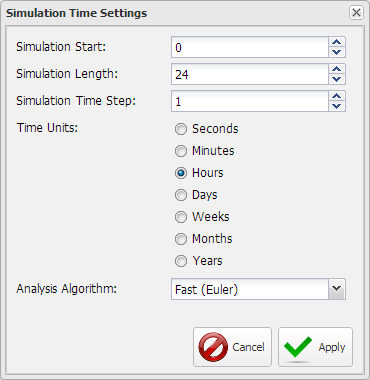
\includegraphics{02-im-4990f.png}
\caption{Figure 9. Time Settings}
\end{figure}

\subsubsection{Simulation Results}

When you click the \u{Run} button the model is stepped through the
defined time period and produces a display of the results as depicted in
Figure 10. There are various options for the type of display and which
elements are displayed as shown in Figure 11.

\begin{figure}[htbp]
\centering
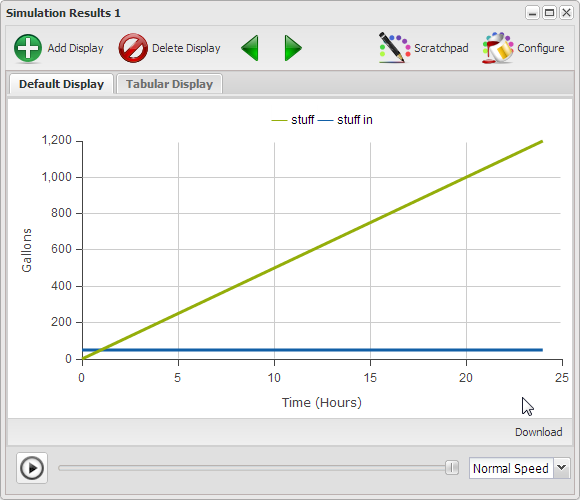
\includegraphics{02-im-4990g.png}
\caption{Figure 10. Simulation Results}
\end{figure}

\subsubsection{Configure Simulation Results}

A default configuration is put together when the model is constructed on
the canvas. If you click the \u{Configure} button in the upper right
corner of the \{Simulation Results\} window the
\u{Chart/Table Configuration} window as depicted in Figure 11 will open.
It is in this window you indicate what type of display you want and
which items of the model are to be displayed. The only part you need to
be concerned about at the moment is the Y-Axis Label field. This where
it was indicated that the items displayed were in Gallons. You will need
to change this shortly in the next exercise.

Note that if you change items in the configuration they will be
immediately reflected in the \u{Simulation Results} window when you
click \u{Apply}. You don't need to run the model again to see a
different configuration of the data. This makes it very convenient when
when you decide you need another display for some items of the model.

\begin{figure}[htbp]
\centering
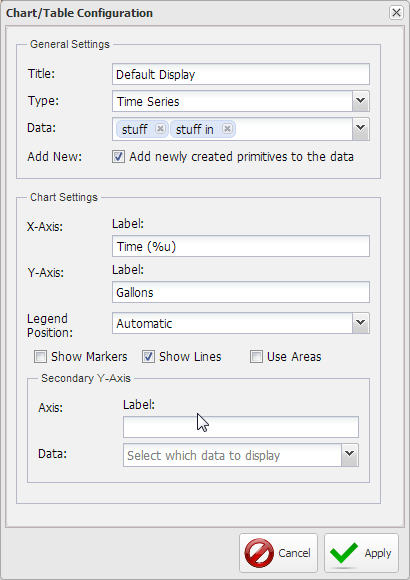
\includegraphics{02-im-4990h.png}
\caption{Figure 11. Chart/Table Configuration}
\end{figure}

Hopefully you haven't found this short introduction to the modeling
environment too overwhelming. Different parts of the environment will be
presented just as you need them to interact with the models presented.

Too much explaining and not enough hands on interaction may get real
boring in a hurry. As such you are encouraged to actually do the
exercises. By interacting with the various aspects of the modeling
environment you will develop a level of comfort and expertise which will
serve you well throughout the rest of the book.

\section{Common Property \# 1}

To this point you've learned how to develop a static picture of a model.
It is actually a model and provides a sense of the relationships between
the various elements. What it doesn't give you a sense of is the dynamic
nature of these over time. What are the implications of the
relationships? In the next few sections you'll learn how to bring your
model to life.

Look at the images in Figure 12 and ask yourself what these images have
in common. The images all represent very different kinds of things, some
living, some not, though there is a characteristic they all have in
common. Have you figured it out?

\begin{figure}[htbp]
\centering
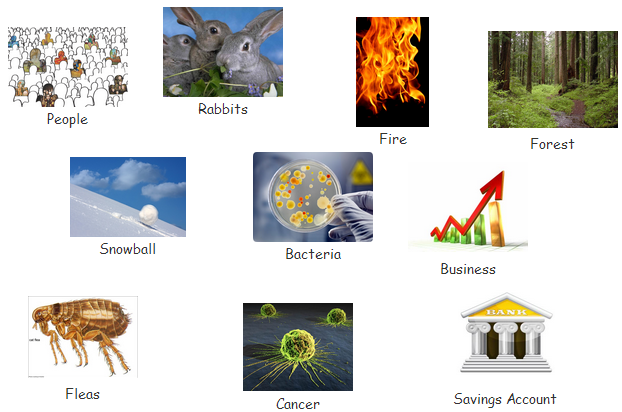
\includegraphics{02-im-4548.png}
\caption{Figure 12. Common Property \# 1}
\end{figure}

Maybe you notice the rabbits from the previous chapter? All the images
represent things that grow over time in one way or another, and some
faster than others.

\section{Reinforcing Growth Structure}

A reinforcing growth structure is one where growth produces a result
which promotes even more growth.

\FloatBarrier 

\begin{model}[frametitle={Model: Reinforcing Growth Model}] 

 We're going to create a generic exponential growth structure for study and reuse.




 \end{model}

\paragraph{}

\beginEx{Exercise 1-1}

Notice that the curve in the previous model is a bit choppy where it
turns up. Run the model with a Time Step of .5, .25, .125, .0625 and
compare the results. What questions are raised by the the results?

\completeEx 

\subsection{Time Units and Time Step Selection}

The \u{Time Units} and \u{Time Step} selected for a model should be
consistent with the time frame and level of detail of the model. You
probably wouldn't develop a model about filling a bathtub with water and
use \u{Time Units} of months. Minutes are probably more appropriate for
this model. The \u{Time Step} is then selected to ensure none of the
relevant transitions associated with the dynamic nature of the model are
missed. A \u{Time Step} of .25, meaning 15 seconds for a model with
\u{Time Units} in minutes, is probably sufficiently small to ensure
there are no transitions missed.

Trial is actually the most appropriate approach to determine if you have
an appropriate value for \u{Time Step}. If you think .5 is appropriate
then run the model with 1, .5, and .25 and if the results for 1 and .25
don't differ from .5 then you're probably OK. If .25 produced a
different result then compare the .25 result with the .125 result. Once
you get two runs where the values don't change then use the larger
value.

\hyperdef{}{Ex-1-2}{\paragraph{}\label{Ex-1-2}}

\beginEx{Exercise 1-2}

Given this guidance how would you interpret the results you experienced
in the previous exercise?

\hfill{} \hyperref[Ans-1-2]{Answer Available}

\completeEx 

One aspect of trying to model the contexts of Figure 12 that should have
become apparent is that there is a piece of the model that's missing.

\FloatBarrier 

\begin{model}[frametitle={Model: Feedback Dependent Growth with Control}] 

 We're now going to add a factor to the previous model so you can control the extent to which the stock influences the flow.




 \end{model}

\hyperdef{}{Ex-1-3}{\paragraph{}\label{Ex-1-3}}

\beginEx{Exercise 1-3}

Using the Feedback Dependent Growth model to implement the models does
this structure allow you to construct more realistic representations of
the growth situations presented in Figure 12? Why?

\hfill{} \hyperref[Ans-1-3]{Answer Available}

\completeEx 

\hyperdef{}{Ex-1-4}{\paragraph{}\label{Ex-1-4}}

\beginEx{Exercise 1-4}

Imagine that the feedback dependent growth model is actually a Savings
Account that is defined as compounding annually, i.e.~calculating and
adding interest once a year. This means that the most appropriate
\u{Time Units} would be years with a \u{Time Step} of 1. There are no
other transitions in this model that need to be accommodated. If you run
this model with any \u{Time Step} other than 1 it will result in a less
accurate result. Why does this happen?

\hfill{} \hyperref[Ans-1-4]{Answer Available}

\completeEx 

This model just developed is the standard reinforcing growth model
depicted at the beginning of this chapter. In the process of arriving at
this model the linear growth was developed first, and then evolved.
Hopefully through the exercises to this point you have gained a deeper
understanding of how this structure works and the extent to which it may
be applied to various situations.

\section{Constructing a Balancing/Goal Seeking Structure}

A Balancing/Goal Seeking structure is one where there is a difference
between two values and the activity of relationships works to develop a
balance between the two values. Essentially what the structure does is
move the \p{Current} value to the value of the \p{Goal}. \FloatBarrier 

\begin{model}[frametitle={Model: Balancing/Goal Seeking Model}] 

 As we have done repeatedly to this point we begin with a linear model consisting of a flow and a stock, along with a flow rate variable. To this we simply have to add a goal and the appropriate feedback and we end up with a goal seeking model.




 \end{model}

\paragraph{}

\beginEx{Exercise 1-5}

Run the above model with various values for factor. What do you notice
about the relation between \p{Current} and \p{Gap}? And what do you
notice about the curves as the factor gets larger and larger?

\completeEx 

Under Time Units and Step Selection we talked about it being essential
that the the \u{Time Units} were selected appropriate to what was being
modeled. In this case since it's a generic model one Time Unit is pretty
much as appropriate as any other. The Time Step is another matter
though, or is it? We said one chooses a Time Step such that none of the
relevant interactions are missed and the change from one Time Step to
another doesn't change the result.

\paragraph{}

\beginEx{Exercise 1-6}

Set up the previous model to run with Current = 0, Goal = 1, and factor
= .75. Now run the model with a Time Step of 1, .5. 25. .125. Does the
result actually change? Look at the Tabular Display associated with the
Simulation Result. As you make the Time Step smaller and smaller are the
results more correct?

\completeEx 

Considering that we don't know anything about a real environment being
modeled it's a bit difficult to determine if the result is actually more
correct as the Time Step used is smaller and smaller.

You might have also realized by this point that it would be quite
difficult if we attempted to use this model to model any of the
situations depicted in Figure 13. While progress toward the goal in the
situations depicted is promoted by the Gap between the Goal and Current
the change in those situations isn't likely to be proportional to that
Gap.

\section{Work Completion Model}

The following model presents a modification to the previous model where
the factor has been replaced by a constraint. It looks like there have
been lots of changes though they all cosmetic except the way Workers
influence work on a daily basis.

\FloatBarrier 

\begin{model}[frametitle={Model: Work Completion Model}] 

 In this model \p{Workers} is not a factor but a limit on the amount of \p{work} that can be performed in a time period.




 \end{model}

Note that in this model you might have considered the \p{Workers} as a
\p{Stock} as they are actually a collection. The reason they're not
considered as a \p{Stock} in this model is that the number remains
constant in the context of this particular model. In a different model
\p{Workers} might actually be a \p{Stock} with an inflow and and
outflow.

\paragraph{}

\beginEx{Exercise 1-7}

Set up the above model to run with Time Step of 0.5. Compare the results
of this run with the results of the previous run above. By making the
time step smaller have we improved the accuracy of result? Why?

\completeEx 

Again the appropriate Time Step is one that captures the activity
occurring within the model. In this case the Workers are in integers and
Project Work in days, both of which are in integers, and with the Time
Units in days the appropriate Time Step is 1. If there were events which
happened in the model on the order of hours then you would have to
decide whether to alter the model to run in hours or reduce the Time
Step to ensure it was small enough so no interactions in the model were
missed.

\paragraph{}

\beginEx{Exercise 1-8}

Use the previous model and reconfigure it for a couple of the activities
depicted in Figure 13. Note that for this exercise you will have to
relabel the stock, flow, and variables accordingly. You will also have
to decide on the most appropriate Time Units and Time Step to use.

\completeEx 

\section{Summary}

Hopefully this chapter has helped you become more familiar with the
modeling environment and the four model elements you will use most
often.

\begin{itemize}
\itemsep1pt\parskip0pt\parsep0pt
\item
  \textbf{Stock}. An accumulation of something that can only be changed
  by something flowing into or out of it.
\item
  \textbf{Flow}. Something moving over time which adds to a stock or
  subtracts from a stock.
\item
  \textbf{Variable}. Constant or equation computed each time the
  simulation steps.
\item
  \textbf{Link}. Used to communicate a value from a Stock, Flow, or
  Variable, to a Stock, Flow or Variable. The source is not changed and
  a link to a stock can only be used to set it's initial value.
\end{itemize}

Because of the nature of the building blocks themselves there are only a
small number of valid connections as depicted in valid connections
model.

These valid connections are used to create only three different types of
structures, linear growth, goal seeking and reinforcing growth. If you
are comfortable with these you should be relieved to know that's all
there are. Just three simple structures will be used for all the models
you will ever build. Of course at times there may be quite a few of
these connected together though you should be confident that you know
about the pieces.

The models that you have experienced in Chapter 1 and Chapter 2 are
referred to as Stock \& Flow Simulation Models. They are also referred
to as quantitative models because of the values associated with the
simulation of these models. In the next chapter we'll investigate a
number qualitative models which are also used in developing
understanding. These are referred to as qualitative models because there
are no numerical values associated with them, though there are times
when they can be quite useful.

\chapter{A Model Is A Model Is A Model}

In previous chapters you worked with what is referred to Stock \& Flow
Simulation Models. These are also referred to as quantitative models
because of the numerical values associated with them. While there are
other types of quantitative models in this text we're focusing on Stock
\& Flow Simulation Models. There is also a class of models referred to
as qualitative models because they have no numeric values associated
with them. There is a level of understanding well served by qualitative
models. This chapter will serve to acquaint you with a couple types you
can create with Insight Maker and are likely to be useful in your study
of systems.

The models presented in this chapter are presented as images because
they're really just pictures and not simulations. Links are provided if
you want to access the sample models directly in Insight Maker.

As we've said repeatedly, models are simplifications of some aspect of
the world around us intended to help us understand something. The Stock
\& Flow Simulation Models are very explicit as they the relations are
represented by numerical formulas and the model may be iterated over
time. The models presented in the sections of this chapter may also
assist in understanding situations though only from a relationship
perspective. There are generally no numerical values associated with
these model and they are not iterated over time.

\section{Rich Pictures}

A Rich Pictures is a pictorial representation of a set of relationships
intended to convey a level of understanding about those relationships
and the implication of those relationships. The strength of Rich
Pictures is that there are no rules associated with creating a Rich
Picture. This means you create the picture that helps you understand the
relationships.

The model in Figure 1 is intended to represent the relationships for a
Savings Account. It is created using the Picture Primitive connected
together with Links.

\begin{figure}[htbp]
\centering
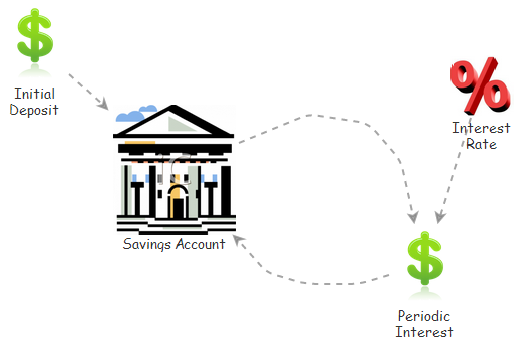
\includegraphics{03-im-7085a.png}
\caption{Figure 1. Rich Pictures/Part 1}
\end{figure}

Picture Primitives are added to the canvas like any of the other
Primitives. Just click on the Primitive to select it then click on the
canvas where you want the Picture to be. You don't have to be too
specific about the placement as items are very easy to move around on
the canvas.

Once the Picture Primitive is placed on the canvas there are several
options available on the \u{Configuration Panel}.

\begin{figure}[htbp]
\centering
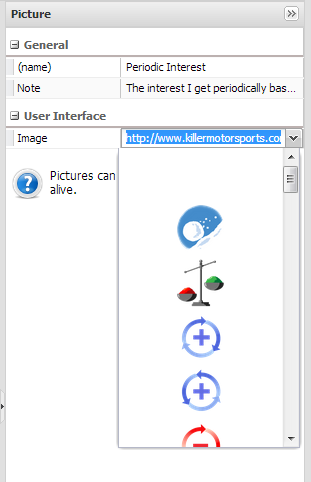
\includegraphics{03-im-7085.png}
\caption{Figure 2. Picture Primitive Configuration Panel}
\end{figure}

The General section of the Picture Primitive is just like the Primitives
you've used to this point with a \a{(name)} and \a{Note} parameters. The
Image option in the User Interface section is new. Here you may select
one of the built in pictures from the drop down menu, no picture, the
first option on the menu, or paste a URL into the field which points to
some graphic on the Internet. Note that the Internet option only works
if you're connected to the Internet.

Once you've created the Picture simply use the Link element to connect
them together as you did in the Stock \& Flow models. After you select
the Link tool and when you mouse over a Picture Primitive the small
right arrow will appear in the center as the connection point. Simply
click on the selection point and drag to the Primitive you want to
connect to. You can't use Flows to connect Picture Primitives.

Note that you can use \p{Stocks}, \p{Variables}, \p{Converters} and
\p{Text} in Rich Pictures. You can add images to all of them except
\p{Text}. Even though this is the case most of the time using Picture
Primitives will serve just fine. We'll talk about Buttons somewhere
further along the way.

\paragraph{}

\beginEx{Exercise 2-1}

Use the Picture Primitive and create a rich picture similar to Figure 1
and connect the Pictures together using the Link tool. Note that in the
Configuration segment of the Configuration Panel for the Link there is
an option to indicate whether a Link is bi-directional. Use some of
these in your exercise.

\completeEx 

The Text primitive is similar to any other primitive in that you select
it then click on the canvas where you want the Text to appear. Once you
create the text item you can edit the text, assign notes to it, connect
to or from it with links, and style it with commands form the Style
segment of the Toolbar.

In this version of the model we add a {[}Folder{]} and a {[}Link
Label{]} to Rich Picture/Part 1.

\begin{figure}[htbp]
\centering
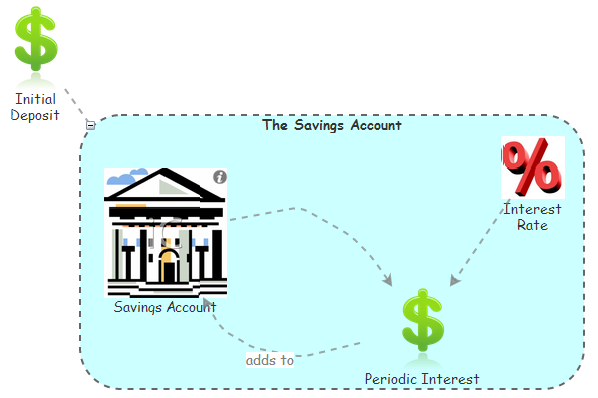
\includegraphics{03-im-7094.png}
\caption{Figure 3. Rich Pictures/Part 2}
\end{figure}

If you select the Link that has the \a{adds to} label on it you'll
notice that the \a{(name)} field in the Configuration Panel contains the
displayed \a{adds to} label and there's text in the \a{Note} field.
These two attributes are like other Primitives. If the \a{(name)} field
is blank or named \a{Link} it won't display. Any other text in the field
will display on the Link, or near it if the link is segmented and
curved. If you segment the Link the program doesn't really know where
you want the label to be. As such if you select the link you'll see a
small yellow node on the text. You can click on this node and move the
label to wherever you would like it to be. Be warned that at times the
positioning is a bit artful, though you'll readily get the knack of it.

Folders are provided so you can enclose a number of items you want to
explicitly draw attention to as a concept and have the ability to hide
the detail if you choose. To hide the detail click on the little minus
(-) sign in the upper left corner of the folder. when you do this the
folder closes, displays it's name and the minus (-) sign changes to a
plus (+) sign. And you probably also surmised when you closed the folder
that you can select an image for a folder or provide an image URL.

Remember the intent of a model is to be some simplification of the world
around you to promote understanding. And while there are really no rules
for creating a Rich Picture, if you want others to understand one you
might want to ensure it is easily understandable rather than confusing.
How is the best way to ensure this? Present it to others and have them
let you know where they think it is clear and where they think it is
confusing. Then go work on it some more.

\section{Causal Loop Diagrams}

A Causal Loop Diagram is more structured than a Rich Picture and less
structured than a Stock \& Flow Diagram. The Causal Loop Diagram was
initially invented as a way to express the findings of a Stock \& Flow
simulation model without having to show the entire simulation model as
it was expected it might overwhelm the audience.

While a Causal Loop Diagram is a qualitative model there is still much
one can come to understand from one because of the information presented
about the relations in one.

We begin with a model of the most basic relations between two elements
of a model.

\begin{figure}[htbp]
\centering
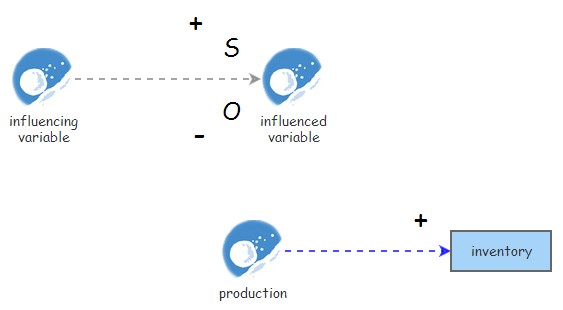
\includegraphics{03-im-7100.png}
\caption{Figure 4. Causal Loop Diagrams/Part 1}
\end{figure}

The good news is there are no new aspects of Insight Maker you need to
learn to create a Causal Loop Diagram. The diagram is created with
\p{Stocks}, \p{Variables}, \p{Pictures} and \p{Links} with \p{Text} used
to indicate the relationship between influencing variables and the
influenced variables. After you create the elements, which you may
represent with the {[}Stock\}, \p{Variable}, \p{Picture} or \p{Text}
\u{Primitives} you use \u{Links} to connect them together and identify
the relationship represented by the \u{Link}.

There are two widely used notations associated with Causal Loop
Diagrams, both of which are presented below.

The first notation popularized by Senge in The Fifth
Discipline\{Cite:Senge, P. 1980. The Fifth Discipline: The Art and
Practice of the Learning Organization.
http://www.amazon.com/Fifth-Discipline-Practice-Organization-ebook/dp/B000SEIFKK/\}
uses an \textbf{S} and \textbf{O} notation as depicted in Figure 4.

\begin{itemize}
\itemsep1pt\parskip0pt\parsep0pt
\item
  \textbf{S} implies that the influenced variable changes in the same
  direction as the influencing variable. If the influencing variable
  increases the influenced variable increases. If the influencing
  variable decreases the influenced variable decreases.
\item
  \textbf{O} implies that the influenced variable changes in the
  opposite direction as the influencing variable. If the influencing
  variable increases then the influenced variable decreases. If the
  influencing variable decreases then the influenced variable increases.
\end{itemize}

The influence indicators are created as Text elements and positioned as
you deem appropriate to represent the influence representative of the
Link.

The \textbf{+} and \textbf{-} notation is an older notation and each has
two possible meanings which are deduced from the context of the diagram.

\begin{itemize}
\itemsep1pt\parskip0pt\parsep0pt
\item
  \textbf{+} implies that the influenced variable changes in the same
  direction as the influencing variable or the influencing variable adds
  to the influenced variable.
\item
  \textbf{-} implies that the influenced variable changes in the
  opposite direction as the influencing variable or the influencing
  variable subtracts from the influenced variable.
\end{itemize}

The \textbf{+} and \textbf{-} notation are considered less likely to
generate inconsistencies in a model when there are elements such as
production and inventory are depicted. In this relationship the
\textbf{+} interpreted as \textbf{adds to} for production adds to
inventory. The situation is such that as production increases inventory
increases and as production decreases inventory still increases, just
not as rapidly. This should allow you to easily see that the \textbf{S}
notation might result in a misinterpretation of the diagram as
production decreases inventory decreases. To aid in avoiding the
confusion some people use \p{Stocks} in their Causal Loop Diagrams to
indicate those elements which are actually accumulations.

Because creating the \u{Link} indicators can get tedious in a hurry
after you create the first one it's much easier to hold down the
\u{Control Key} then click on the indicator and drag to a new location.
This quickly creates you a copy of the indicator. You can actually use
this sequence to duplicate any element, or selection of elements, of a
model.

As this section is about Causal Loop Diagrams there probably should be
some loops defined here somewhere shouldn't there? Figure 6, Causal Loop
Diagrams/Part 2, presents a Causal Loop of the Balancing and Reinforcing
loops presented in Chapter 1 and Chapter 2.

\begin{figure}[htbp]
\centering
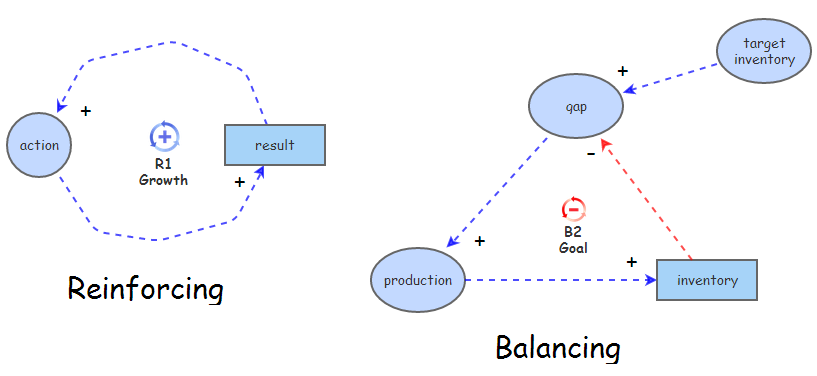
\includegraphics{03-im-7101.png}
\caption{Figure 5. Causal Loop Diagram/Part 2}
\end{figure}

The Balancing and Reinforcing models presented vary slightly from
typical causal loop diagrams in the following ways.

\begin{itemize}
\itemsep1pt\parskip0pt\parsep0pt
\item
  \textbf{Variables}. Variables in a Causal Loop Diagram are typically
  just Text though here we've used Stocks for those variable which
  represent accumulations and Pictures, with no images, to represent the
  variables. The advantage in using Picture elements for variables is
  that there are no restrictions on labels because Picture elements are
  never used in equations.
\item
  \textbf{Link Colors}. Because the Link identifiers have to be created
  separately and are not attached to the Link it's much easier to make
  \textbf{+} indicators Blue and \textbf{-} indicators Red. This seems
  to be an evolving convention and when used you could just leave the
  Link indicators out altogether.
\end{itemize}

While models are a simplification of the world around you intended to
promote understanding they also represent an unfolding story. It is
appropriate to sequence and label the loops. This gives others a guide
to what order to read the story and the intent of the loop itself. The
images are created with Picture elements and the images for reinforcing
\textbf{+} and balancing \textbf{-} loops, both clockwise and
counterclockwise are defined images available from the pull images pull
down on the \p{Picture} \u{Configuration Panel}.

The easiest way to identify whether a loop is a reinforcing or balancing
loop is to count the number of minus (-) influences around the loop. If
the number is zero or even then the loop is a reinforcing loop. If the
number is odd then it's a balancing loop.

\section{Hybrid Models}

There are times when the message you want to get across may be best
represented by a combination of Rich Picture and Causal Loop forms as
depicted in Figure 6.

\begin{figure}[htbp]
\centering
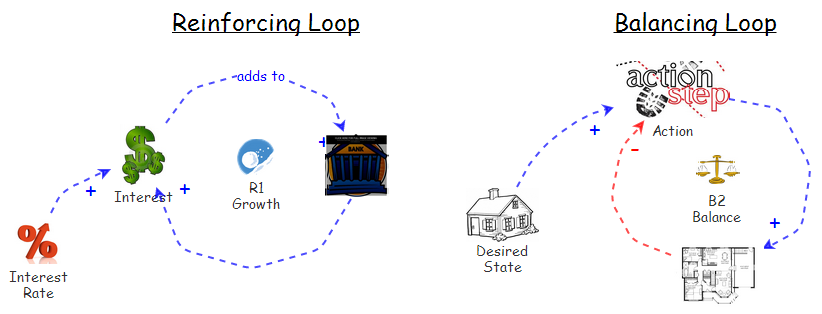
\includegraphics{03-im-7102.png}
\caption{Figure 6. Hybrid Model}
\end{figure}

If the images make it easier for the model to develop and convey
understanding then it helps them achieve their purpose. The model in
Figure 7 presents a Hybrid Causal Loop Diagram for The Boy Who Cried
Wolf Aesop's Fable.

\begin{figure}[htbp]
\centering
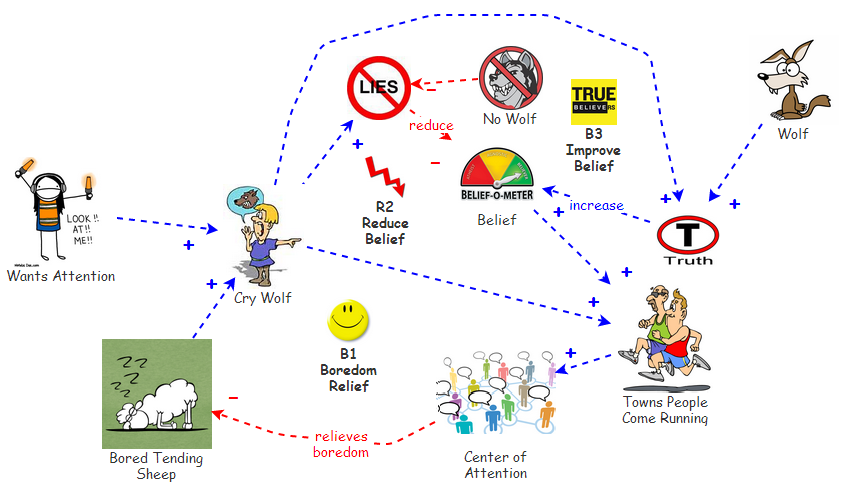
\includegraphics{03-im-7103.png}
\caption{Figure 7. The Boy Who Cried Wolf}
\end{figure}

In the next section you will be introduced to the Unfolding feature of
Insight Maker which you can use to build a script so the model will
explain itself to someone else when you're not there.

\section{Storytelling}

Even though you may conscientiously develop your model and add comments
often it turns out that people initially look at the whole model and are
immediately overwhelmed. It might be somewhat like trying to eat a whole
Elephant in a single bite. Storytelling provides a way to overcome this
difficulty.

Storytelling a model is intended to reveal a model little by little and
explain it along the way. Click on the View Story button in the lower
left corner of the screen, read the text, and then click the Step
Forward arrow on the right repeatedly to have the model presented as a
story.

Adding a story to a model is very straight forward and is initiated by
clicking \u{Add Story} in the \u{Tools} section of the \u{Toolbar}. This
opens the \u{Story Designer} which is described as follows.

\begin{figure}[htbp]
\centering
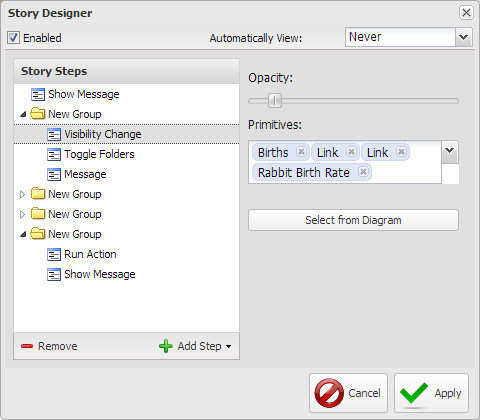
\includegraphics{03-im-7104.png}
\caption{Figure 8. Story Designer}
\end{figure}

The main elements of this window are\ldots{}

\begin{itemize}
\itemsep1pt\parskip0pt\parsep0pt
\item
  \textbf{Enabled}. This check box allows you to actually enable
  Storytelling. If this box is checked the green plus sign and View
  Story will show up in the lower left corner of the window.
\item
  \textbf{Automatically View}. There are four options on this drop down
  allowing you to indicate the conditions under which View Story should
  execute automatically when the model is opened. The options are Never,
  For Editors, For Non-Editors, Always.
\item
  \textbf{Story Steps}. Lists the steps that you have defined as part of
  the story. You may reorder steps by clicking and dragging them to the
  new location. If you click on one of the steps it's definition will be
  displayed on the right side of the Story Designer window. Currently
  the definition of the first Visibility Change is displayed.
\item
  \textbf{- Remove}. To remove an Story Step first click on it to select
  it then click the \textbf{- Remove} button.
\item
  \textbf{+ Add Step}. A drop down which allows you to select which type
  of step you want to add. New steps are added after the currently
  selected step. If the new step is not created where you want it just
  select it and drag it to the location in the sequence where you want
  it. The various steps will be described shortly.
\item
  \textbf{Cancel}. Allows you to exit the Story Designer and not save
  any changes.
\item
  \textbf{Apply}. Applies all the changes you have made in the Story
  Designer and exits.
\end{itemize}

There are five different types of steps you can include in a story.

\begin{figure}[htbp]
\centering
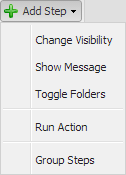
\includegraphics{03-im-7104a.png}
\caption{Figure 9. Steps of a Story}
\end{figure}

When you select any one of these steps it will be added after the
currently selected step in the list. As the following step types are
described you might want open the Story Designer and click on different
Unfolding Steps to visualize how they're defined.

\begin{itemize}
\itemsep1pt\parskip0pt\parsep0pt
\item
  \textbf{Change Visibility}. Allows you to specify the Opacity, with
  the slider, for one or more elements of the model when the step is
  executed. The steps may be selected from the drop down or you may
  select one or more items from the model and then click the
  \textbf{Select from Diagram} button to put those items in the list.
  Note that clicking the \textbf{Select from Diagram} button will
  replace the already selected elements with whatever you've selected in
  the model. If you want to add or remove one more more Primitives it's
  probably better to use the drop down to add or click the existing item
  to remove it.
\item
  \textbf{Show Message}. Allows you to enter a text message you want to
  be displayed. There are some formatting options available in the
  Message edit window.
\item
  \textbf{Toggle Folders}. Use this option to Expand or Collapse one or
  more folders. This is really useful if you want to expand a folder,
  walk through the items in the folder and then close the folder.
\item
  \textbf{Run Action}. Provides you with a window in which you can enter
  Javascript commands to control various aspects of the model. There are
  a large number of functions in the
  \href{http://insightmaker.com/sites/default/files/API/files/API-js.html}{Insight
  Maker API} that you can employ in this step.
\item
  \textbf{Group Steps}. This step creates a folder in the sequence in
  which you can place multiple steps. This allows you to indicate there
  are several steps you want to execute with a single Next Step click.
  You can see how this was used in the Figure 8 definition of an
  unfolding. You can open and close a New Group folder by toggling the
  little triangle to the left of it. Also if you click on a folder you
  can rename it in the \textbf{Name} field on the right.
\end{itemize}

By creating a story of your model you significantly increase the
likelihood that others will understand the insights your model is
endeavoring to surface. You might even find that in the process of
creating the story you uncover ways to improve or clarify the model for
yourself.

The following storytelling examples may be viewed by opening the model
and repeatedly clicking \textbf{Step Forward} in the bottom right of the
model.

\FloatBarrier 

\begin{model}[frametitle={Model: Rabbit Population}] 

 The rabbit population model demonstrates exponential growth.





\begin{enumerate}[label=\protect\circled{\arabic*}] \setcounter{enumi}{0}

\item The model diagram should now look something like this: \par \begin{minipage}{\linewidth}  \centering 
\includegraphics{model_17/diagram_2.png}
\end{minipage}




 \end{enumerate} 


 \end{model}

\FloatBarrier 

\begin{model}[frametitle={Model: The Boy Who Cried Wolf}] 

 Short term actions are defeated by the longer term response.





\begin{enumerate}[label=\protect\circled{\arabic*}] \setcounter{enumi}{0}

\item The model diagram should now look something like this: \par \begin{minipage}{\linewidth}  \centering 
\includegraphics{model_18/diagram_2.png}
\end{minipage}




 \end{enumerate} 


 \end{model}

\FloatBarrier 

\begin{model}[frametitle={Model: Systems Thinking: The Essence of And?}] 

 To uncover the system one must continue to seek out the inflences.





\begin{enumerate}[label=\protect\circled{\arabic*}] \setcounter{enumi}{0}

\item The model diagram should now look something like this: \par \begin{minipage}{\linewidth}  \centering 
\includegraphics{model_19/diagram_2.png}
\end{minipage}




 \end{enumerate} 


 \end{model}

\section{Summary}

Always remember that a model is a simplification of the world around you
intended to help you understand something. You should use a modeling
form that adequately serves your quest for understanding. Stock \& Flow,
Rich Picture, and Causal Loop models are only three of a very large
array of possible modeling forms that exist. Use them to the extent that
they serve you and when they don't find a form that does. The Modeling
and Simulation references provide access to several additional types of
diagrams that have been created with Insight Maker, though there are
probably more that haven't yet been identified. The Model Thinking
Course by Scott E. Page presents a very extensive exposure to many types
of models useful for understanding different aspects of the world around
us.

\subsection{Rich Pictures}

\begin{itemize}
\itemsep1pt\parskip0pt\parsep0pt
\item
  Often easier for others to relate to and understand because of the
  images in the model.
\item
  No rules for creating them though remember that you need to tell a
  story.
\item
  Because you need to tell a story make the model as understandable as
  possible.
\end{itemize}

\subsection{Causal Loop Diagrams}

\begin{itemize}
\itemsep1pt\parskip0pt\parsep0pt
\item
  Specific Guidelines for how to depict the relationships between the
  elements.
\item
  Two conventions for expressing relations.
\item
  S and O notation can produce misinterpretations when it comes to
  stocks.
\item
  The older + and - notation is considered more appropriate.
\item
  Color coding relations is an alternative to both notations, though be
  consistent.
\item
  Employing explicit stock representations often reduces
  misinterpretations.
\item
  Hybrid Rich Pictures/Causal Loop Diagrams are often the very
  meaningful.
\end{itemize}

\subsection{Storytelling}

\begin{itemize}
\itemsep1pt\parskip0pt\parsep0pt
\item
  Makes it far easier for others to understand the insights you're
  trying to surface with your model.
\end{itemize}

\section{References}

\begin{itemize}
\itemsep1pt\parskip0pt\parsep0pt
\item
  \href{http://www.amazon.com/Fifth-Discipline-Practice-Organization-ebook/dp/B000SEIFKK/}{Senge,
  P. 1990. The Fifth Discipline: The Art \& Practice of the Learning
  Organization}
\item
  \href{http://www.systemswiki.org/index.php?title=Modeling_\%26_Simulation_with_Insight_Maker}{Modeling
  \& Simulation with Insight Maker}
\item
  \href{https://www.coursera.org/course/modelthinking}{Model Thinking
  Course} by Scott E. Page, University of Michigan
\item
  \href{http://systems.open.ac.uk/materials/T552/pages/rich/richAppendix.html}{Rich
  Pictures} from Open University Course T552
\end{itemize}

\chapter{Building a Model}

\begin{lstlisting}
“Would you tell me, please, which way I ought to go from here?”
“That depends a good deal on where you want to get to,” said the Cat.
“I don’t much care where–” said Alice.
“Then it doesn’t matter which way you go,” said the Cat.
“–so long as I get SOMEWHERE,” Alice added as an explanation.
“Oh, you’re sure to do that,” said the Cat, “if you only walk long enough.”

Lewis Carroll - Alice in Wonderland
\end{lstlisting}

Now that the most relevant aspects of Insight Maker have been introduced
it is appropriate to provide you with a meaningful process and
guidelines to use when you set out to build a model to promote an
understanding of an area of interest. An aspect of this essential for
the development of sound models is the topic of units. While units don't
ensure a model is sound, if the units don't match up one can be certain
the model is not sound.

\section{Model Construction Process}

We develop models to help us understand the implications of
interactions, and sometimes guidance. As such, as with Alice above, it
is essential that before you begin to build a model you know what it is
that you want to understand otherwise how will you know if the model
does what you needs to do.

There are a number of guidelines or rules of thumb that you will find
helpful when developing a model. These will be presented as Modeling
Tips throughout this chapter. The idea is to ensure that the model
serves the purpose you started building it for.

\begin{figure}[htbp]
\centering
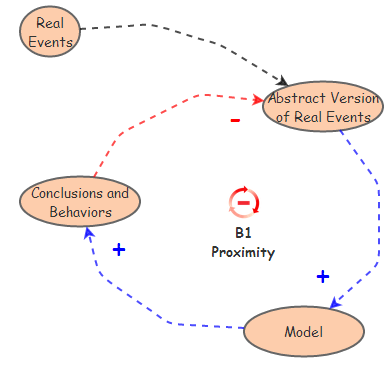
\includegraphics{04-im-184.png}
\caption{Figure 1. Model Construction Process}
\end{figure}

The difference between \p{Real Events} and \p{Conclusions and Behaviors}
result in the creation of an \p{Abstract Version of Real Events}. The
abstraction is then used to develop a \p{Model} which promotes a
revision to \p{Conclusions and Behaviors}. This cycle continues until
the \p{Model} produces a set of \p{Conclusions and Behaviors} which are
congruent with \p{Real Events}. At this point there's no longer a need
to create an \p{Abstract Version of Real Events}, meaning you have
achieved the understanding you were seeking.

The model construction process of Figure 1 is very conceptual. As you
continue to develop models you will arrive at a sequence that you are
comfortable with an enables you to achieve the understanding your
seeking.

The following two figures present the two model formulation processes
presented by Andrew Ford in Modeling the Environment\{cite: Ford, A.
2009. Modeling the Environment.
http://www.amazon.com/Modeling-Environment-Second-Edition-Andrew/dp/1597264733/\}

\begin{figure}[htbp]
\centering
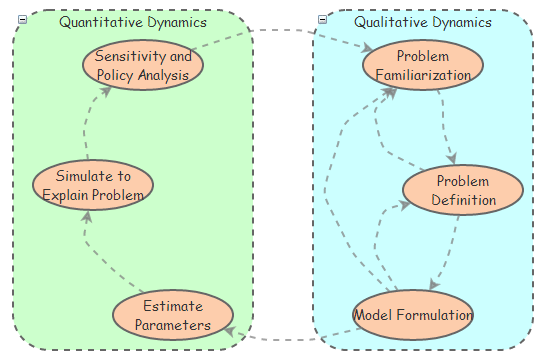
\includegraphics{04-im-220.png}
\caption{Figure 2. Emphasis on Model Formulation}
\end{figure}

In approach presented in Figure 2 one focuses on the understanding the
qualitative dynamics, i.e., problem familiarization, problem definition
and model formulation. Not until such time as there is a level of
comfort in the understanding of these dimensions, which may employ Rich
Pictures or Causal Loop Diagrams, does one progress to the quantitative
aspect of model building, i.e., estimating parameters, simulating to
explain the problem and sensitivity and policy analysis, which is where
the Stock \& Flow simulation model is employed. The quantitative
dynamics may produce sufficient understanding or the process may
continue back into the qualitative dynamics area. Model development is
an iterative process.

Figure 3, which may look like complete chaos, emphasizes simulation to
provide feedback to provide a better understanding of all other aspects
of the modeling process.

\begin{figure}[htbp]
\centering
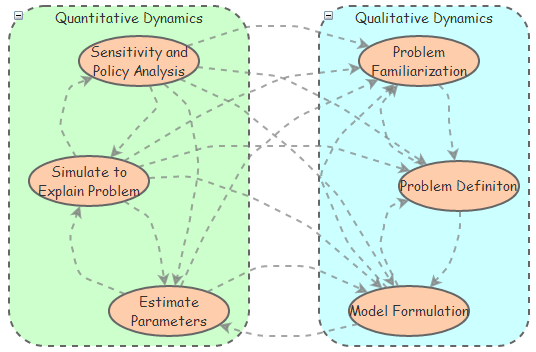
\includegraphics{04-im-219.png}
\caption{Figure 3. Emphasis on Simulation Early \& Simulate Often}
\end{figure}

Here the belief is that actually simulating all stages of the model are
the best way to ground one's understanding of all other aspects of the
model development process.

As you develop models you will develop an approach which is probably
somewhere between Figure 2 and Figure 3 that you are comfortable with.
That is probably the most critical aspect, i.e., that you be comfortable
with your process and it make sense to you and helps you understand.

\section{Modeling Guidelines}

Figure 4 presents a number of guidelines or rules of thumb it would be
good for you to keep in mind as you develop models. Some of the
following are only relevant to Stock \& Flow simulations, and which they
are should be quite obvious.

\begin{figure}[htbp]
\centering
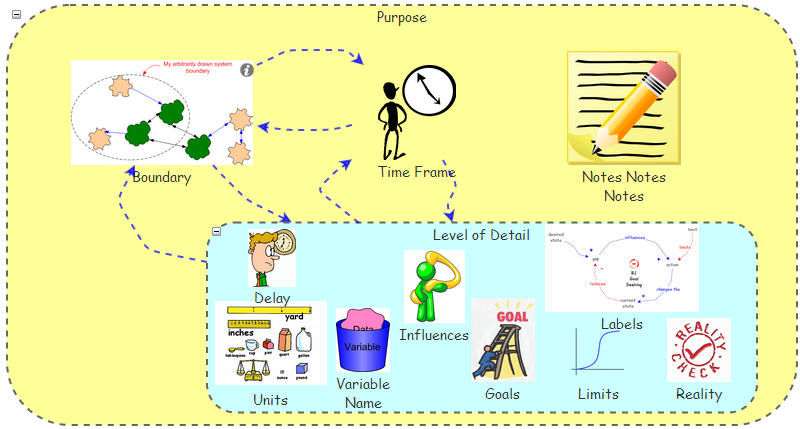
\includegraphics{04-im-1784.png}
\caption{Figure 4. Modeling Guidelines}
\end{figure}

Remember that model development and the understanding that comes with it
is an iterative process. It's almost impossible to create all the pieces
as they should be the first time around. Look at it as do a little,
learn a little, and repeat.

\begin{itemize}
\itemsep1pt\parskip0pt\parsep0pt
\item
  \textbf{Purpose}. Have a sense of what you want the model to
  accomplish and expect the thought to evolve as you develop the model.
\item
  \textbf{Boundary}. A boundary allows you to explicitly define what's
  part of the model and what's not part of the model. If you're unclear
  on the purpose of the model and unable to establish a boundary how
  will you ever know when to stop adding things to the model?
\item
  \textbf{Time Units}. Will the interactions in this model be depicted
  over Years, Months, Days, etc. And you should realize that you initial
  thought may have to be revised once you begin developing the model.
\item
  \textbf{Simulation Length}. How long might the interactions have to be
  modeled for. Here again the answer may be obvious, or you may have to
  start with an estimate and revise it after working with the model.
\item
  \textbf{Time Step}. Here again you have to estimate a value based on
  the smallest time of transition you expect in the interactions and
  then test it to see if you you're close enough.
\item
  \textbf{Notes Notes Notes}. As you build your model add notes to the
  elements so you can refer back to them later to get a sense of what
  you were thinking when you created them. Yes, you tell yourself you
  know what you're doing at the moment, though you'll be surprised at
  what you won't remember a week, a month or even a year from now. Notes
  also make it much easier for others to understand what you intended
  when you created elements.
\item
  \textbf{Variable Names}. A stock represents a quantity and should be
  labeled with a directionless noun our noun phrase, you know, a person,
  place or thing. Avoid directional modifiers such as increasing,
  decreasing, growing, slowing, etc. as they tend to make a model very
  difficult to understand. A flow represents something moving over time
  so it's label should be something one would easily think of as moving
  over time as walk, speed, flow, etc.
\item
  \textbf{Loop Labels}. If you're developing a Causal Loop Diagram or
  Stock \& Flow Diagram be sure to label and sequence your loops so
  others have a sense in what order to read your story.
\item
  \textbf{Goals}. Balancing loops always have goals. Make sure they're
  explicitly identified.
\item
  \textbf{Influences}. Make sure you include all relevant influences and
  only the relevant influences. Sometimes you include items because you
  can't figure out if they're relevant or not. That's OK as long as you
  remember to later take out the ones that aren't relevant. If you leave
  influenced which aren't relevant they are likely to result in
  confusion later.
\end{itemize}

The following items are most likely relevant only for Stock \& Flow
simulations.

\begin{itemize}
\itemsep1pt\parskip0pt\parsep0pt
\item
  \textbf{Stocks}. Identify which items are the the stocks, or
  accumulations, in the model that will change over time. Stocks are
  often easy to identify if you think about stopping time. When time
  stops a stock still has a quantity. In this case it's the distance
  from Grandma's house as Red walks toward it.
\item
  \textbf{Flows}. Identify the flows which are responsible for changing
  the stocks over time. If time stops a flow has no value. In this case
  it's walking.
\item
  \textbf{Delay}. Delays can have very unexpected impacts on the
  behavior of a model. Where there are delays make sure they're
  explicitly identified.
\item
  \textbf{Units}. Units can be very instrumental in assuring model
  validity. While consistency of units doesn't guarantee model validity
  if the units are inconsistent you can be sure the model is not valid.
\item
  \textbf{Limits}. If there are limits on Stocks, Variables or Flows be
  sure they are explicitly stated so Insight Maker can inform you if the
  model generates out of limit value. This will signal you that there is
  a problem with assumptions or initial values.
\item
  \textbf{Reality Check}. Ensure the model is producing results which
  are consistent with reality. If it is not then it's an opportunity for
  learning.
\end{itemize}

The guidelines are far too much to memorize though if you refer to them
as a check list over time they will actually become second nature and
you'll find yourself checking them as you're adding elements to a model.

\section{Can Red Get to Grandma's House}

Here's a simple example of a question that might be answered with a
model. And yes, it is quite obvious you could just do the math though
would you get any better at building models if you did?

\section{Setting Units}

If you click on the stock and look at the configuration panel you'll
notice that the last item in the list, \a{Units}, has a value of
unitless. Units were not addressed in the first three chapters as they
are so important we wanted to ensure we could provide them the focus
they deserve. You use units to help ensure that your models are sound.
Not that units will guarantee that your model is sound, though if the
units don't work out right you can be sure there's a problem, so Insight
Maker checks them for you.

Figure 5 shows the Configuration Panel for the stock where Units is
assigned a value of miles. For this particular model miles makes sense
as we're trying to figure out how long it takes Red to get to Grandma's
House and we know it's 4.5 miles away.

\begin{figure}[htbp]
\centering
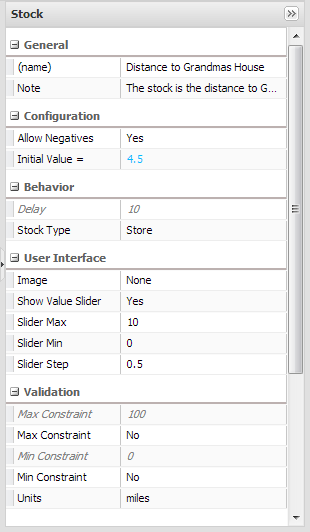
\includegraphics{04-im-6767.png}
\caption{Figure 5. Units for Distance to Grandma's House in miles}
\end{figure}

If you click on the flow and look at the configuration panel you'll
notice that the Units for walk is miles/hour as depicted in Figure 6. A
flow represents the movement of something during a time period which is
why this is 1/hours.

\begin{figure}[htbp]
\centering
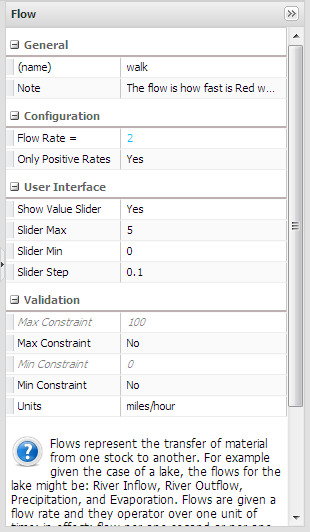
\includegraphics{04-im-6767a.png}
\caption{Figure 6. Units for Walk is in miles/hour}
\end{figure}

The flow has a units of hours as that's what will be set up in
\u{Time Settings} as the \u{Time Units} for the model. All the time
settings are shown in Figure 7.

\begin{figure}[htbp]
\centering
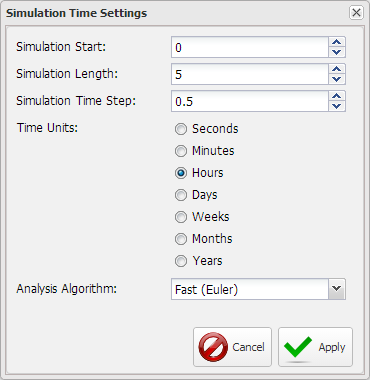
\includegraphics{04-im-6767b.png}
\caption{Figure 7. Time Settings for Walk to Grandma's House}
\end{figure}

You might now be asking, how the \p{Walk} in miles/hour gets turned in
to \p{Distance to Grandma's} in miles? Because we've selected a
\a{Time Step} of 0.5 each simulation step multiplies 0.5 hours x 2
miles/hour to get 1 mile traveled each time step. And the units are
consistent. Later you can try changing the \u{Time Units} and running
the model to see how that affects the answers. It's not actually this
simple though with a constant flow rate this description is close
enough.

\begin{center}\rule{3in}{0.4pt}\end{center}

\subsection{Modeling Tip}

There are a large number of units predefined in Insight Maker. If you
click in the Units field and then click on the drop down on the right
the \u{Units Selection} window will open as depicted in Figure 8. Here
you can select from predefined units, though it's usually easier to just
enter the appropriate units into the \a{Units} field. There is also a
way to define Custom Units thought we'll cover this option in a later
chapter.

\begin{figure}[htbp]
\centering
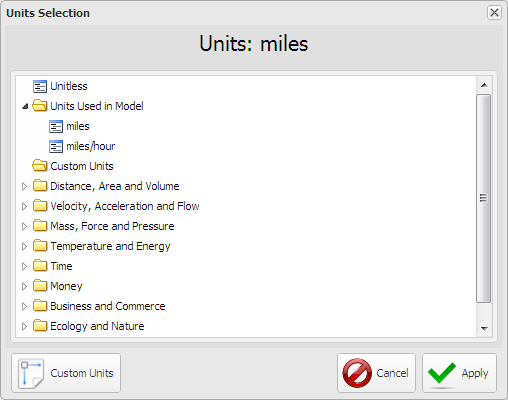
\includegraphics{04-im-6767e.png}
\caption{Figure 8. Units Selection}
\end{figure}

\begin{center}\rule{3in}{0.4pt}\end{center}

\FloatBarrier 

\begin{model}[frametitle={Model: Stopping At Grandma's}] 

 We'll begin with the previous model and add an option that tells the model to stop when Red actually gets to Grandma's.




 \end{model}

If you look at the \u{Configuration Panel} for \p{Stop at Grandmas}
you'll notice that the \a{Units} are unitless. The variable itself
doesn't need a definition of units because it's not participating in any
calculations. It's just a test.

As for the formula what you should remember is that when you start using
units in a model, which you should do, all formulas have to be
consistent from a units perspective otherwise Insight Maker will raise
an error message. Just as a test change \{0 miles\} to 0 and run the
model. Because {[}Distance to Grandmas House{]} has units what it is
compared to has to have units.

\hyperdef{}{Ex-3-1}{\paragraph{}\label{Ex-3-1}}

\beginEx{Exercise 3-1}

In the {[}Stop at Grandmas{]} variable change \{0 miles\} to \{0
kilometers\}. Does the model still work? Why?

\hfill{} \hyperref[Ans-3-1]{Answer Available}

\completeEx 

\hyperdef{}{Ex-3-2}{\paragraph{}\label{Ex-3-2}}

\beginEx{Exercise 3-2}

Seldom is there ever just one right way to build a model. You build the
model to help you understand something and you might do that in
different ways. Even for a model as simple as Going to Grandma's can be
structured in several different ways other than starting with a stock of
2.5 and reducing it by walking. Try to build one or two alternatives to
this model.

\hfill{} \hyperref[Ans-3-2]{Answer Available}

\completeEx 

Hopefully the Going to Grandma's model has given you a sense of an
approach for developing models along with some useful tips and an
introduction to using units and why they can be so useful to you. Oh,
and don't forget about putting notes in your models. Wiring diagrams
without knowing what the pieces mean are generally not very useful.

\section{Why Aren't We All Rich}

If one can put money in an investment account and it grows over time,
and it grows even faster with regular deposits, why aren't more people
rich and ready for retirement? I've started numerous retirement programs
through the years though for one reason or another they've all
evaporated in time. What is the basis of this sad state of affairs?

The following is intended to be another example of he development of a
model, though somewhat more involved than the previous one. Here's the
initial question describing what I'd like to understand.

This figure presents the initial set up for this model.

\begin{itemize}
\itemsep1pt\parskip0pt\parsep0pt
\item
  \textbf{Investment Account}. represents the amount of money, in
  Dollars, in the account. If you look at the Configuration Panel you'll
  notice that Units are set to Dollars.
\item
  \textbf{Initial Deposit}. is a variable used to specify the amount of
  money that is initially put into the {[}Investment Account{]} when it
  is opened. Remember we said only a flow can increase or decrease a
  stock, though you can use a external variable to set the initial value
  for a stock. This is done done to make the {[}Initial Deposit{]}
  explicit with a slider for testing. The Units for {[}Initial
  Deposit{]} is also set to Dollars.
\item
  \textbf{Time Setting}. We've assumed that this is an investment
  account that will compute and add interest on a monthly basis so the
  time settings are set up to run for 36 months with an initial Time
  Step = 1 knowing that we will have to test this later on.
\end{itemize}

\begin{center}\rule{3in}{0.4pt}\end{center}

\subsection{Modeling Tips}

Before you run a model you should develop a sense of the result you
expect from the model at this point in its development. Once you run the
model you should be certain that is it performing as expected. When the
result is not what you expect then either the structure is wrong, your
assumptions are wrong, or you simply have an opportunity to further
develop your understanding.

You should never be more than a single concept change away from a
running model that produces a result that you understand. You may think
this a bit strict though after you add several elements to a model and
it doesn't work and you spend hours trying to figure out why you may
have a better appreciation for this guideline.

Making all the elements of a model visible makes it much easier for
others to understand it. This is why Months per Year and Initial Deposit
were created as explicit variables rather than embedding the valued
inside other elements.

And what's definitely worth repeating is that providing comments for all
the elements of a model will also make it much easier for others to
understand. All one need do is mouse over an element and click on the
``i'' that appears to read the comment.

You have the option of adding notes to the Picture element and there are
a number of predefined images that you can select from the pull down
that can be assigned to the element. There are images for balancing and
reinforcing loops, both clockwise and counter clockwise. These pictures
can be assigned to Variables and Stocks also.

The other option is that you can put a URL in this field for an image
somewhere on the web and that image will be displayed and may be
resized.

\begin{center}\rule{3in}{0.4pt}\end{center}

\textbf{Penalty} is levied by the Government if the funds are withdrawn
before you reach 59 1/2 and is meant to be an encouragement to save. The
\% Penalty is a variable with a slider defined to you can test the value
during runs. The Units for Penalty are Dollars/Month.

\textbf{Withdrawal} represents money taken out of the account to
purchase things with. As the amount of money in the Investment Account
grows it becomes more and more attractive for use to purchase other
things and there develops a tug of war between the Attractiveness of the
money in the Investment Account and one's Determination to Save.
Attractiveness and Determination to Save both represented by percentages
between 0 and 100\%. Attractiveness is represented with a Converter, a
modeling element not previously described.

\begin{center}\rule{3in}{0.4pt}\end{center}

\subsection{Modeling Tip}

It is often the case that a variable to be used in a model can not be
represented as a constant or some well defined formula. The variable is
actually a function of Time or some other variable. In the case of this
model Attractiveness is a function of Investment Account and is defined
as a set of data points.

The next figure shows the Configuration Panel for Attractiveness
Principle. Note that many of the configuration options are the same as
other modeling elements. The ones that are different are in
Configuration and Input/Output Table.

\begin{figure}[htbp]
\centering
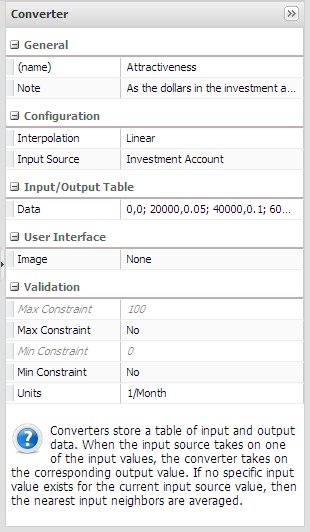
\includegraphics{04-im-6827.png}
\caption{Figure 9. Attractiveness Control Panel}
\end{figure}

Because the variable is defines as a set of XY coordinates the Data has
to be defined point by point as depicted below, or the table may be
imported.

\begin{figure}[htbp]
\centering
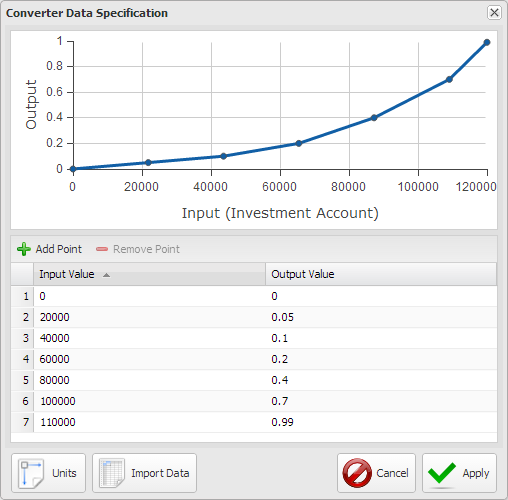
\includegraphics{04-im-6827a.png}
\caption{Figure 10. Attractiveness Data Specification}
\end{figure}

Also notice on the Converter Configuration Panel there is an option for
Interpolation. This option defines how Insight Maker figures out the Y
values in between the defined X points. The graph displayed in Figure 21
depicts the Linear Interpolation meaning that Insight Maker treats the
line between two points as a straight line and if computes the Y value
from the XY values at the two points on either side of the X value.

Figure 11 shows the curve for the Interpolation option of None meaning
that it treats all the Y values between point X1Y1 and X2Y2 as Y1.

\begin{figure}[htbp]
\centering
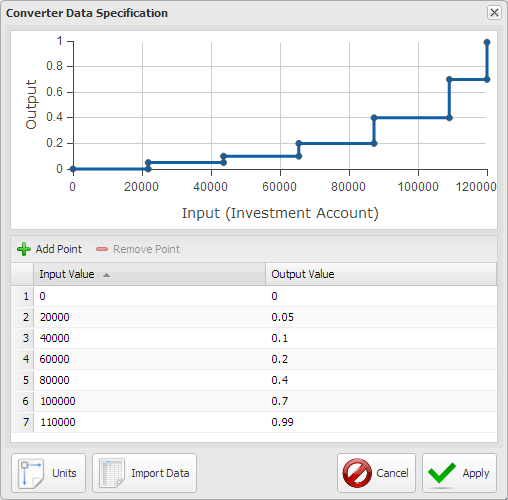
\includegraphics{04-im-6827b.png}
\caption{Figure 11. Attractiveness Data Specification with Interpolation
= None}
\end{figure}

\begin{center}\rule{3in}{0.4pt}\end{center}

The following figures show the various display tabs for a run of this
model with a Determination to save of 50\%.

\begin{figure}[htbp]
\centering
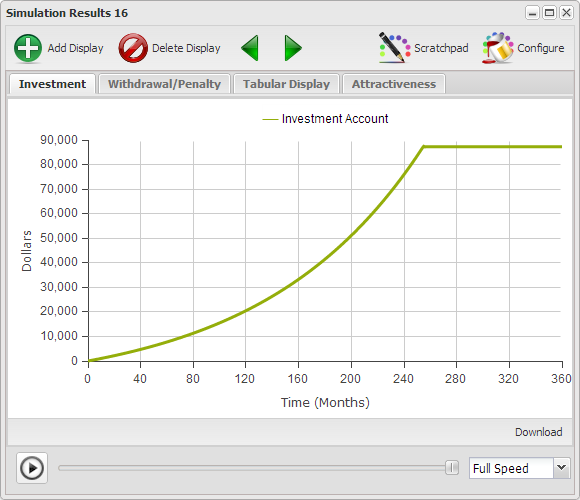
\includegraphics{04-im-6827c.png}
\caption{Figure 12. Investment Account Limited by Attractiveness}
\end{figure}

When the Investment Account reaches \$87,000 dollars after 255 months it
is sufficiently attractive to overcome the Determination to Save so
money is withdrawn from the account every month and the account no
longer grows. Is this a bad thing? That depends on the intent.

\begin{figure}[htbp]
\centering
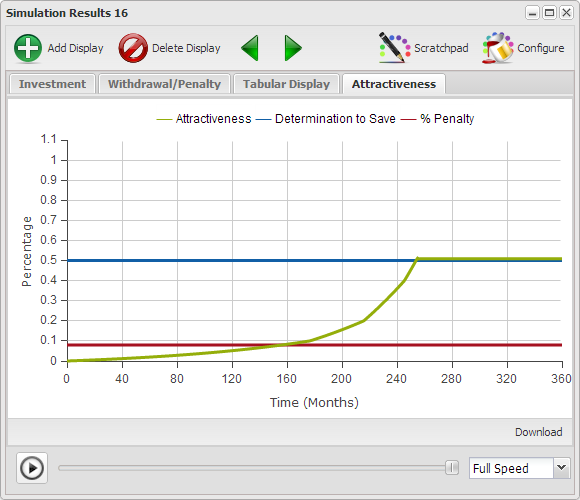
\includegraphics{04-im-6827d.png}
\caption{Figure 13. Investment Account Attractiveness and Determination}
\end{figure}

Figure 24 just shows that the Attractiveness has reached the
Determination to Save level so withdrawals begin happening every month.

\begin{figure}[htbp]
\centering
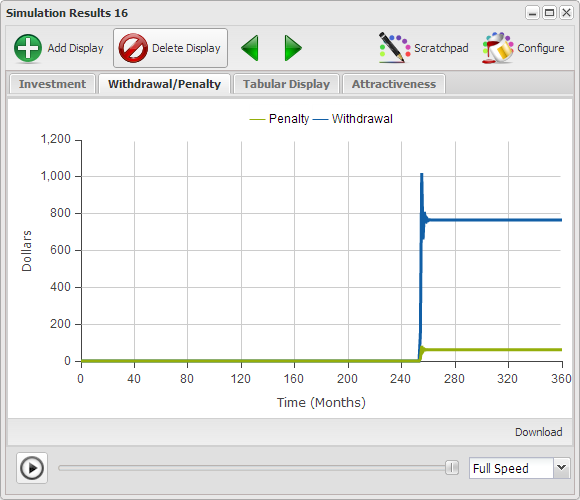
\includegraphics{04-im-6827e.png}
\caption{Figure 14. Investment Account Withdrawal and Penalty}
\end{figure}

The above figure shows that there is almost \$800 dollars a month being
withdrawn from the account monthly and the account doesn't decrease.
Maybe it's accomplishing what it needs to if \$800 a month is sufficient
to augment other income.

Note the large overshoot on the Withdrawal curve and a small one on the
Penalty curve. This is most likely because the Time Step is too large.
The next figure is the same display tab for the model run with a Time
Step of 0.5. Notice how the curve cleans up.

\begin{figure}[htbp]
\centering
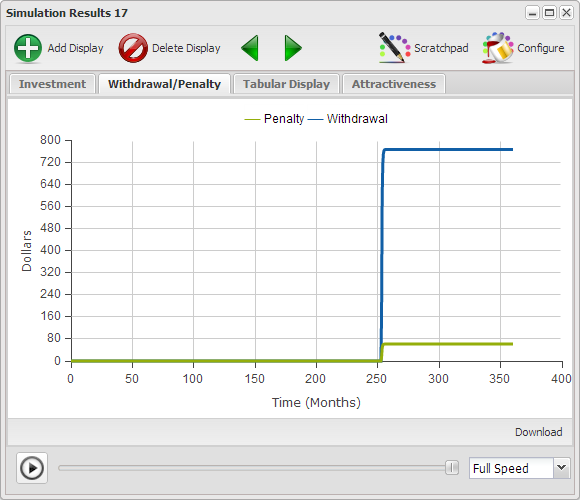
\includegraphics{04-im-6827f.png}
\caption{Figure 15. Investment Account Withdrawal and Penalty with Time
Step = 0.5}
\end{figure}

\begin{center}\rule{3in}{0.4pt}\end{center}

\subsection{Exercise 3-4}

There is a logic flaw in this model which you might try to repair. The
Penalty is not actually taken from the Investment Account but from the
Withdrawal itself so it reduces the amount you actually get from the
Withdrawal. Be warned that is might be a tricky fix.

\begin{center}\rule{3in}{0.4pt}\end{center}

We now have a model which provides some incentives to start and continue
to deposit in an Investment Account, and some disincentives toward the
withdrawal of funds, though have we really addressed the initial
situation posed? Not really. As far as starting the Investment Account
and regularly depositing money, there are incentives, and for many these
incentives were enough to get them to invest. For many the incentive,
for one reason or another, has not been sufficient. And, any more strict
incentives would likely be looked on unfavorably. People do not like to
be manipulated, even when it is for their own benefit. The penalty for
withdrawal is a deterrent in some respects though as the Investment
Account continues to grow its attractiveness in terms of what it can
purchase continues to entice. The best answer for this situation is to
legally tie up the withdrawal process so it's only an option in the case
of dire emergencies. Though as much as people find being manipulated by
others distasteful, being controlled by themselves is just as
distasteful.

Is the model done? As usual, the answer is; ``It Depends!'' If it has
provided sufficient understanding to address the situation posed then it
is sufficient. If not then it should be taken further, though once it is
sufficient you should STOP!

\section{Where Have All The Trees Gone?}

We had a forest reserve of over a million trees and the logging company
guaranteed us they would plant a new tree for every one they cut down,
yet all of a sudden there are no trees left to harvest. What happened?

\FloatBarrier 

\begin{model}[frametitle={Model: Where Have All The Trees Gone}] 

 Investigating the implications of different time horizons.





\begin{enumerate}[label=\protect\circled{\arabic*}] \setcounter{enumi}{0}

\item The model diagram should now look something like this: \par \begin{minipage}{\linewidth}  \centering 
\includegraphics{model_21/diagram_2.png}
\end{minipage}




 \end{enumerate} 


 \end{model}

\hyperdef{}{Ex-3-3}{\paragraph{}\label{Ex-3-3}}

\beginEx{Exercise 3-3}

What have you come to understand about the difference between short term
and long term perspectives and how do delays figure into surprises?

\hfill{} \hyperref[Ans-3-3]{Answer Available}

\completeEx 

\section{Moose and Wolves Revisited}

In Chapter 1 a model which revealed the dynamic relationship between the
population of Moose and Wolves. The model is presented here with an
exercise to test your intuition.

\FloatBarrier 

\begin{model}[frametitle={Model: Moose and Wolves Revisited}] 

 The populations of Moose and Wolves are dynamically linked.




 \end{model}

\hyperdef{}{Ex-3-4}{\paragraph{}\label{Ex-3-4}}

\beginEx{Exercise 3-4}

What would you expect to happen in the Moose and Wolves model if there
were no Moose or no Wolves? Open the model and run it for each
situation.

\hfill{} \hyperref[Ans-3-4]{Answer Available}

\completeEx 

\section{Building a Model Summary}

\begin{itemize}
\itemsep1pt\parskip0pt\parsep0pt
\item
  \textbf{Intent}. Be sure you have a good idea of what you want the
  model to help you understand. This may evolve as you develop the
  model.
\item
  \textbf{Time Frame}. Ensure you have a sense of the time frame over
  which you intend to simulation the model. As you build the mode you
  may find you need to adjust your initial thought on this.
\item
  \textbf{Stocks \& Flows}. Identify the Stocks \& Flows first as they
  are key elements of the model.
\item
  \textbf{Use Units}. Units help to ensure your model is sound and
  Insight Maker will test for consistency of units. If the units are
  consistent it doesn't guarantee the model is sound though it does add
  a level of confidence.
\item
  \textbf{Variables \& Links}. Add Variables \& Links to influence the
  flows.
\item
  \textbf{Test Often}. Each time you make a logical addition to the
  model think about how you expect the model to behave then run the
  model and see if there is agreement with your expectation. If it isn't
  then it's an opportunity to learn and improve the model. And if it
  does agree you should still consider the output. It may be that your
  expectation and the model are both wrong.
\item
  \textbf{Time Step}. Test the Time Step to ensure it's small enough to
  capture all relevant transitions in the model.
\item
  \textbf{Stop at the End}. When the model serves the purpose for which
  you are developing it, STOP! There is always more you can add to a
  model. You should only include what is relevant to satisfy the initial
  intent.
\end{itemize}

\section{References}

\begin{itemize}
\itemsep1pt\parskip0pt\parsep0pt
\item
  Catalina Foothills School District. 2003. Tips for Using System
  Dynamics Tools.
  \url{http://www.clexchange.org/ftp/documents/Implementation/IM2003-12TipsUsingSDTools.pdf}
\item
  Ford, Andrew. 2009. Modeling the Environment.
  \url{http://www.amazon.com/Modeling-Environment-Second-Andrew-Ford/dp/1597264733/}
\item
  Keeting, Elizabeth K. Internet 2013. Everything You Ever Wanted to
  Know about How to Develop A System Dynamics Model, But Were Afraid to
  Ask.
  \url{http://www.systemdynamics.org/conferences/1998/PROCEED/00024.PDF}
\item
  Newell, Barry \& Proust, Katrina. 2012. Introduction to Collaborative
  Conceptual Modelling.
  \url{https://digitalcollections.anu.edu.au/bitstream/1885/9386/3/Newell_IntroductionCollaborative_2012.pdf}
\item
  Whiftield, Caraig. 2012. What Returns Should We Expect from the Stock
  Market. \url{http://www.whitfieldco.com/blog/?p=39}
\end{itemize}

\chapter{Frequently Recurring Structures}

Chapter 1 presented Bertalanffy's premise that that the same basic
structures operated across all disciplines, and if one learned how these
structures operated one could transfer much of their learning from one
discipline to another. In the previous chapters there has been a focus
on three basic structures in support of Bertalanffy's premise. In this
chapter will will build on those three basic structures in such a way as
to demonstrate that there exists a set of more complex structures
composed of combinations of the basic three which also repeatedly occur
across all disciplines of science.

\section{Basic Structures}

The three basic structures are depicted in Figure 1 along with their
characteristics behavior curves in Figure 2.

\begin{figure}[htbp]
\centering
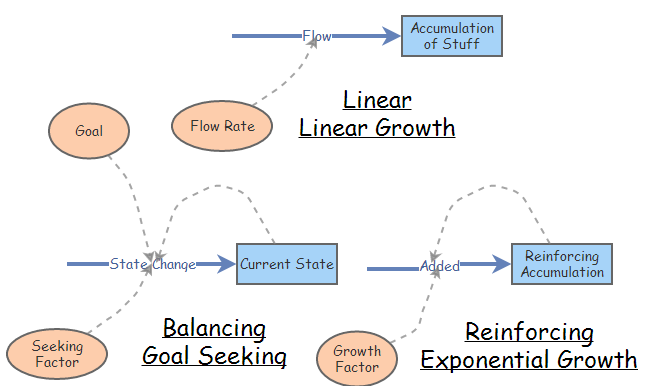
\includegraphics{05-im-5138.png}
\caption{Figure 1. Three Basic Structures}
\end{figure}

\begin{figure}[htbp]
\centering
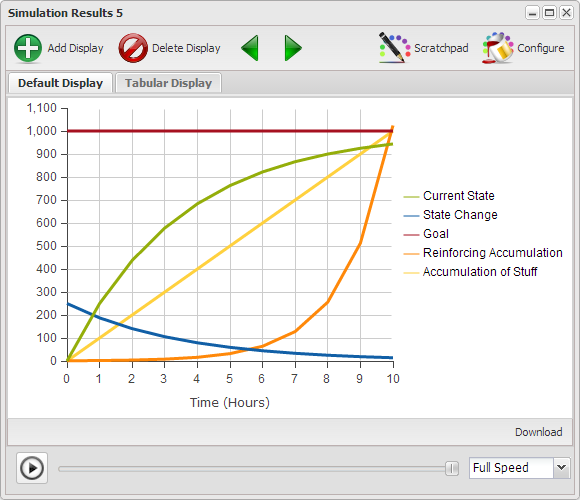
\includegraphics{05-im-5138a.png}
\caption{Figure 2. Three Basic Structures Behavior}
\end{figure}

In the Chapter 1 and Chapter 2 we covered these three basic structures
in some detail and it was claimed that all the models you will ever
create will simply be a combination of some number of these basic
structures. We don't expect that you take this on faith, and while we
can't prove it, this chapter, and the next two, will provide you an
opportunity to experience some of the more common structures which
repeatedly occur across all disciplines of science.

\section{Typical Evolving Relationships}

When you undertake something it is either to fix a problem, represented
by the Balancing/Goal Seeking structure, or promote growth represented
by the Reinforcing/Exponential Growth structure. Seldom will you
encounter either of these structures in their elementary form. Typically
there are multiple structures interacting and even if you create an
elementary structure is it likely to readily evolve into a more complex
form. Figure 3 depicts the manner in which the Balancing/Goal Seeking
and Reinforcing/Exponential Growth structures tend to be found as part
of, or evolve into, more complex structures. Each structure has a
characteristics pattern of behavior, which in conjunction with its
structure, helps to identify the particular structure.

\begin{figure}[htbp]
\centering
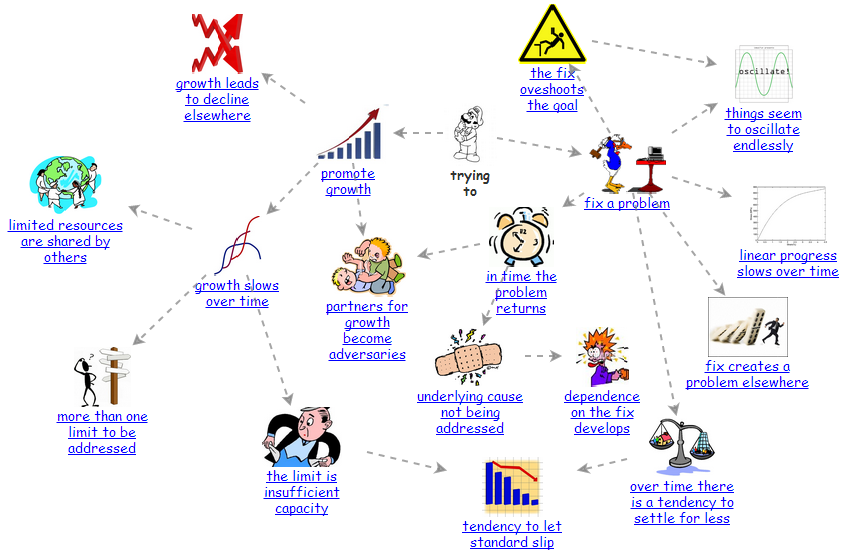
\includegraphics{05-im-538.png}
\caption{Figure 3. Typical Evolving Relationships}
\end{figure}

\section{Summary}

The chapter provides an introduction to the explicit relationships
between the most commonly recurring structures along with their natural
evolution paths. The next two chapters will provide a detailed
investigation of these structures along with their characteristic
pattern of behavior which will help you recognize and address them.

\section{References}

\begin{itemize}
\itemsep1pt\parskip0pt\parsep0pt
\item
  Bellinger, Gene. 2013. Systems Archetypes.
  \url{http://www.systemswiki.org/index.php?title=Systems_Archetypes}
\item
  Braun, Bill. 2002. The Systems Archetypes.
  \url{http://wwwu.uni-klu.ac.at/gossimit/pap/sd/wb_sysarch.pdf}
\end{itemize}

\chapter{Common Balancing Structures}

The sections of this chapter will present an investigation of the more
frequently experienced balancing structures and their characteristic
patterns of behavior. Links will be provided at the end of the chapter
to allow you to continue investigation of those structures not presented
here.

Each structure will be presented in a generic form so you can focus on
the implications of the relationships rather than what the actual
elements are. Each section will also provide appropriate strategies for
dealing with the structure as well as a number of explicit example of
this structure in different areas.

Because the Balancing/Goal Seeking structure has already been presented
we'll simply begin with more complex structures.

\section{Linear Progress Slows Over Time}

A Limits to Results structure represents a situation where a Balancing
Loop moving toward its goal is slowed in its progress due to some
limiting factor. This is generally due to some resource restriction or
constraint.

\FloatBarrier 

\begin{model}[frametitle={Model: Limits to Results}] 

 A balancing loop seldom progresses simply based on the difference between the \p{current state} and the \p{desired state}.




 \end{model}

\hyperdef{}{Ex-5-1}{\paragraph{}\label{Ex-5-1}}

\beginEx{Exercise 5-1}

\begin{itemize}
\itemsep1pt\parskip0pt\parsep0pt
\item
  Run the model with different values for limit. What difference do you
  see in the curve when the limit is evenly divisible into 1.
\item
  What happens if you change the Time Step to 0.5, 0.25 and 0.125. What
  is the most appropriate value to use for Time Step?
\end{itemize}

\hfill{} \hyperref[Ans-5-1]{Answer Available}

\completeEx 

\subsection{Examples}

Numerous example for this structure should readily come to mind.

\begin{itemize}
\itemsep1pt\parskip0pt\parsep0pt
\item
  Any undertaking to complete a project is restricted by the
  availability of resources.
\item
  The flow of anything to fill or empty a stock is restricted by the
  capacity of what the liquid must flow through.
\item
  The rate of production of a process is limited by the capacity of the
  process.
\end{itemize}

\subsection{Effective Strategy}

\begin{itemize}
\itemsep1pt\parskip0pt\parsep0pt
\item
  The effective way to avoid a Limits to Results scenario is simply to
  plan ahead to ensure there are sufficient resources available so
  progress toward results is not limited to a greater extent than
  acceptable. That said, remember that more of a good thing is not
  always the best answer. There is often a trade off and more resources
  may cost more than one gains by reducing the time by using more
  resources. There's always more than one thing that should be
  considered.
\end{itemize}

\section{The Fix Overshoots the Goal}

Have you ever pursued a goal and later found that you actually overshot
the goal and had to back up to get back to the goal? The Balancing Loop
with Delay structure is a variation of the standard Balancing Loop. The
variation being that there are one or more delays in the structure which
are responsible for producing, as will be demonstrated, a very different
behavior pattern than the standard Balancing Loop.

If you look at the Balancing Loop with Delay structure it looks
identical to the standard balancing loop with the exception of the delay
near the reduces link. The implication is that it takes some amount of
time after the current state changes before it is actually realized and
figures into the calculation of the gap which influences the subsequent
action. Essentially what's happening is that action is being based on
old data and therefore is probably not the appropriate action. The
implications of this will become evident when we look at the simulation
for this structure.

\FloatBarrier 

\begin{model}[frametitle={Model: The Fix Overshoots The Goal}] 

 Lets take a look at the implications of varying delays on the effect of a balancing loop.




 \end{model}

You might ask how could it be that it might take 3.5 days for someone to
get a sense of what the results of the previous actions were, which
would be a good question. It's probably difficult to find a situation
where this is realistic in days though what's important to realize is
this structure could operate in this manner if the time units were
hours, minutes, seconds or microseconds.

\paragraph{}

\beginEx{Exercise 5-2}

Run this model varying the values of action factor, time delay and time
step to develop a sense of how each of these variables influences the
behavior of the model.

\completeEx 

\subsection{Examples}

\begin{itemize}
\itemsep1pt\parskip0pt\parsep0pt
\item
  \textbf{Adjusting the Shower}. When you adjust the hot and cold water
  for the shower it takes time for the new mixing ratio to actually be
  felt in the water temperature to it's easy to over compensate due to
  impatience.
\end{itemize}

\subsection{Effective Strategies}

\begin{itemize}
\itemsep1pt\parskip0pt\parsep0pt
\item
  Advice for dealing with this structure is quite simple. Patience is a
  virtue. If you know you're dealing with a balancing structure and
  things are not going as expected then study the structure to see if
  there could be one or more delays that your impatience is simply
  having difficulty dealing with. This structure proves that there are
  times when taking additional action is worse than not taking
  additional action. More is not always better. If things are waffling
  back and forth endlessly or out of control a little less effort might
  be appropriate.
\item
  An alternative is to monitor the Current State on a more frequent
  basis and ensure the result of the monitoring impacts the action
  appropriately in a more timely manner. In short, take the delay out of
  the structure.
\end{itemize}

\section{Over Time There Is A Tendency To Settle For Less}

Have you ever noticed how difficult it is to bring the best of
intentions to fruition? How so many people's New Years resolutions only
last a few days? Our inability to achieve the things we set out to
achieve is very much a result of the operation of a Drifting Goals
structure we generally have little awareness of.

\FloatBarrier 

\begin{model}[frametitle={Model: Drifting Goals}] 

 If it takes an extended period of time to achieve a goal there is a tendency to settle for achieving a lesser goal.




 \end{model}

\paragraph{}

\beginEx{Exercise 5-3}

Vary the \p{pct chg fact}, \p{goal chg fact} and \p{Time Step} values to
get a sense of the impact on the extent to which the goal for the
structure is degraded over time.

\completeEx 

\subsection{Examples}

\begin{itemize}
\itemsep1pt\parskip0pt\parsep0pt
\item
  New years resolutions. Need I say more?
\item
  Weight loss programs.
\end{itemize}

\subsection{Effective Strategies}

\begin{itemize}
\itemsep1pt\parskip0pt\parsep0pt
\item
  There is only one real effective way to deal with this structure,
  which is to disconnect the feedback from tension to goal reduction to
  Desired State so it can no longer subtract from Desired State.
\item
  An alternative strategy is to further increase the action toward the
  Current State so it reduces the time delay such that there is no time
  for the tension to reduce the Desired State. This is fine if there are
  sufficient resources to increase the action.
\end{itemize}

\subsection{Areas of Concern}

\begin{itemize}
\itemsep1pt\parskip0pt\parsep0pt
\item
  The action toward the Desired State requires resources, which may have
  to be developed. Consideration needs to be given as to whether or not
  there really are sufficient resources to achieve the Desired State.
  For further insights into this see Growth and Underinvestment with a
  Drifting Standard.
\end{itemize}

\section{In Time The Problem Returns}

Have you noticed how often your best intentions go awry? You set out to
fix a problem and shortly thereafter you find yourself fixing the same
problem again, and again. This generally results from some unexpected
consequences, things that come into play because of your action, or the
results of your action, that you never expected, which is why they're
called unexpected consequences.

\FloatBarrier 

\begin{model}[frametitle={Model: Fixes that Fail}] 

 This structure consists of a balancing loop intended to achieve a particular result which is foiled by an insidious reinforcing loop.




 \end{model}

\paragraph{}

\beginEx{Exercise 5-4}

Run the Fixes that Fail structure with various values of action factor,
uc factor, ucd factor, and Time Step to get a sense of how these four
factors influence the behavior of the structure.

\completeEx 

\subsection{Examples}

\begin{itemize}
\itemsep1pt\parskip0pt\parsep0pt
\item
  Your soccer ball is soft so you put air in it though in a few hours
  you have to put more air in it. And after a few weeks it seems like
  you spend all your time pumping up your soccer ball.
\item
  Often times what appears to be the most appropriate way to deal with
  the situation doesn't really solve the problem and in time actually
  makes the situation worse.
\item
  To deal with a cash shortage one often borrows money ensuring there
  will be more cash problems in the future.
\item
  In response to cash flow problems companies often choose to layoff
  employees essentially ensuring they will have more cash flow problems
  in the future.
\end{itemize}

\subsection{Effective Strategies}

\begin{itemize}
\itemsep1pt\parskip0pt\parsep0pt
\item
  The most effective strategy for dealing with this structure is advance
  planning. Since you can never do just one thing, as everything affects
  everything else, before taking action to change the current state,
  think about what else that action, or change in the current state, is
  likely to affect. And, what effect the effect will have. Sometimes the
  unexpected consequence may be several effects away, so don't stop at
  just one. Essentially what one seeks to do is close the loop and
  identify the unexpected, which means it's no longer unexpected then,
  is it?
\item
  A less effective strategy would be to figure out how to disconnect the
  unexpected consequence from influencing the action or the current
  state. Of course then it wouldn't be a consequence, would it?
\end{itemize}

\subsection{Areas of Concern}

\begin{itemize}
\itemsep1pt\parskip0pt\parsep0pt
\item
  There are times when attempts to deal with a situation in a particular
  way makes it even more difficult to deal with the situation in an
  appropriate manner later on which is often an indication of a Shifting
  the Burden Systems Archetype.
\end{itemize}

\section{The Underlying Cause Is Not Being Addressed}

How many times have you noticed that there are some problems that seem
to be addressed over and over. When the problem arises it is addressed,
then some time later, maybe a day, a week, or a month, the same problem
arises again. This situation is quite often the result of a Shifting the
Burden structure.

\FloatBarrier 

\begin{model}[frametitle={Model: Shifting the Burden}] 

 This model demonstrates the difference between treating the symptoms and actually solving the problem.




 \end{model}

\hyperdef{}{Ex-5-5}{\paragraph{}\label{Ex-5-5}}

\beginEx{Exercise 5-5}

While there are myriad of possible variations for the variables in this
model you might find the result interesting if you apply the fundamental
solution without the symptomatic solution. What questions does this
result raise?

\hfill{} \hyperref[Ans-5-5]{Answer Available}

\completeEx 

\subsection{Examples}

\begin{itemize}
\itemsep1pt\parskip0pt\parsep0pt
\item
  Dieting to lose weight rather than changing one's lifestyle results in
  short term weight loss which will only last for a short time. The side
  effect is that the success of the diet removes the perceived need to
  implement the fundamental solution.
\end{itemize}

\subsection{Effective Strategies}

Initially I perceived there to be a single appropriate strategy for
dealing with this structure though I have found examples, which I will
attach as soon as I get them sorted out, which seem support the range of
strategies below.

\begin{itemize}
\itemsep1pt\parskip0pt\parsep0pt
\item
  Learn to live with the symptomatic solution because that's as good as
  it's going to get. There are situations where there may be more
  effective solutions though you'll just never get them implemented in
  your lifetime. Sad but true. -Implement the fundamental solution
  because if the symptomatic solution is implemented the strength of the
  side effect will ensure the fundamental solution will never get any
  traction.
\item
  When dealing with a problem ask yourself if you are treating the
  symptoms or addressing the real cause of the problem. Often, out of
  expediency, the symptomatic solution is essential. The most effective
  strategy for dealing with a Shifting the Burden structure is to employ
  the symptomatic solution AND develop the fundamental solution. Thus
  one resolves the immediate problem and the other works to ensure that
  it doesn't return.
\end{itemize}

\subsection{Areas of Concern}

\begin{itemize}
\itemsep1pt\parskip0pt\parsep0pt
\item
  It is often the case that the side effect promotes some sort of
  dependency which further inhibits development of the fundamental
  solution. For insights into this situation see Addiction Systems
  Archetype.
\end{itemize}

\section{Summary}

The chapter should explicitly depict the relationships between the
structures presented in the previous sections and explain the natural
evolution paths for the structures.

\section{References}

\begin{itemize}
\itemsep1pt\parskip0pt\parsep0pt
\item
  Bellinger, Gene. 2013. Systems Archetypes.
  \url{http://www.systemswiki.org/index.php?title=Systems_Archetypes}
\item
  Braun, Bill. 2002. The Systems Archetypes.
  \url{http://wwwu.uni-klu.ac.at/gossimit/pap/sd/wb_sysarch.pdf}
\end{itemize}

\chapter{Common Reinforcing Structures}

Chapter 1 presented Bertalanffy's premise that that the same basic
structures operated across all disciplines, and if one learned how these
structures operated one could transfer much of their learning from one
discipline to another. In the previous chapters there has been a focus
on three basic structures in support of Bertalanffy's premise. In this
chapter will will build on those three basic structures in such a way as
to demonstrate that there exists a set of more complex structures
composed of combinations of the basic three which also repeatedly occur
across all disciplines of science.

The sections of this chapter will present an investigation of the more
frequently experienced structures and their characteristic patterns of
behavior. Links will be provided at the end of the chapter to allow you
to continue investigation of those structures not presented here.

Each structure will be presented in a generic form so you can focus on
the implications of the relationships rather than what the actual
elements are. Each section will also provide appropriate strategies for
dealing with the structure as well as a number of explicit example of
this structure in different areas.

Because the Reinforcing/Exponential Growth structures have already been
presented we'll simply begin with more complex structures.

\section{Growth Slows Over Time}

A Limits to Growth Systems Archetype consists of a Reinforcing Loop, the
growth of which, after some success, is offset by the action of a
Balancing Loop. As such it may produce exponential growth for a period
of time before the growth slows.

\FloatBarrier 

\begin{model}[frametitle={Model: Limits to Growth}] 

 The natural exponential growth of the reinforcing structure is restricted by a balancing loop.




 \end{model}

\hyperdef{}{Ex-6-1}{\paragraph{}\label{Ex-6-1}}

\beginEx{Exercise 6-1}

The structure provided for Limits to Growth limits growth via a
balancing loop that attempts to move {[}results{]} in the direction of
the {[}limiting factor{]}. How else might you construct a limits to
growth structure.

\hfill{} \hyperref[Ans-6-1]{Answer Available}

\completeEx 

\subsection{Examples}

\begin{itemize}
\itemsep1pt\parskip0pt\parsep0pt
\item
  Rabbits tend to multiply very rapidly so why is it we're not
  completely overrun by rabbits, well maybe everywhere except Australia?
\item
  Keep playing instead of cleaning up the mess in the room, which makes
  further play difficult, AND the increased mess repels one from
  cleaning up.
\item
  An epidemic begins with a infected person
\end{itemize}

\subsection{Effective Strategies}

\begin{itemize}
\itemsep1pt\parskip0pt\parsep0pt
\item
  The best defense is a good offense. As defined in the effective
  strategies for the Reinforcing Loop, if there is a Reinforcing Loop
  operating start looking for what is going to become a limiting factor,
  and remove it before it even has a chance to create a substantial
  impact on the result.
\item
  If the structure is already at a stage where the limiting factor is
  interacting with results to limit results the options are:
\item
  Alter the limiting factor in such a way that it no longer interacts
  with the results to create a slowing action.
\item
  Find a way to disconnect the results from the slowing action so it can
  no longer add to it.
\item
  Disconnect the slowing action from the results so it can no longer
  have a negative impact.
\end{itemize}

\subsection{Areas of Concern}

\begin{itemize}
\itemsep1pt\parskip0pt\parsep0pt
\item
  There are often multiple limits to deal with which leads to an
  Attractiveness Principle.
\item
  It is possible that limited shared resources are the source of the
  limiting factor leading to a Tragedy of the Commons.
\item
  The limit may be insufficient capacity which leads to Growth and
  Underinvestment.
\end{itemize}

\section{Partners for Growth Become Adversaries}

Susan was feeling more than slightly down. She hadn't had a real good
day at school and now was headed for volleyball practice. She wondered
why she stayed on the team since she could hardly remember the last time
they won a game. She realized that winning wasn't everything though
winning once in a while would be nice.

During volleyball practice there was a coaching session where the coach
talked about the difference between all the players pulling together
rather then each trying to be the star player. Susan had heard this
before and was really waiting for the coach to be done so they could get
back to practice.

The coach then did something rather unexpected. The coach gave each of
the eight players on the team a piece of string and asked the players to
try to break it. Susan thought this was rather stupid as she easily
broke the string. Then the coach gave each player a longer piece of
string and asked them to put them all together. Then the coach asked
fours girls to get on each end of the eight strands of strings and try
to break them. As hard as they tried they couldn't break the strings.

The coach then asked what the team had learned. Mary commented that it
looked as though all the strings together were much stronger than the
individual strings. The coach then asked if that might also be true for
the girls when they acted together as a team rather than each one trying
to be the star player. Susan though this a rather striking contrast.

After practice Susan was headed home though rather dreading dinner and
the evening at home as she and her mother had been at odds with each
other all week. As she continued her walk all of a sudden she thought,
maybe her an her mother were having the same problem as the volleyball
team. As she arrived at home and walk in the kitchen she said, ``Mom, I
learned something rather surprising at practice today.''

The situation with the volleyball team and with Susan and her mother is
typically referred to as an accidental adversaries scenario. In this
situation two or more parties who could should be supporting each other
to achieve results are actually working against each other because of
their efforts to promote their own success or position.

The Accidental Adversaries structure represents a situation where two
entities which would be in a synergistic growth relationship end up
limiting each others results because of their own activities.

The problem arises when either A or B does something that promotes their
own success which also acts to inhibit the success of the other. The
other responds with an attempt to compensate for whatever is inhibiting
their success though their action tends to inhibit the success of the
other. As such the two entities that should be cooperating for their
mutual success become adversaries.

\FloatBarrier 

\begin{model}[frametitle={Model: Accidental Adversaries}] 

 When the synergy isn't!




 \end{model}

\hyperdef{}{Ex-6-2}{\paragraph{}\label{Ex-6-2}}

\beginEx{Exercise 6-2}

Why is it that the results balance whenever B to B Ctrl = A to A Ctrl?

\hfill{} \hyperref[Ans-6-2]{Answer Available}

\completeEx 

\subsection{Examples}

\begin{itemize}
\itemsep1pt\parskip0pt\parsep0pt
\item
  Parents can be interesting. Both Mums and Dads want to act as good
  role models and create a positive family environment, but sometimes,
  each one of them gets caught up in being seen as `'the good parent"
  and gives in to our whims and desires. We all know how this works: If
  one parent says 'no' to something, we just ask the other parent. The
  problem is that when one or both of our parents wants to be seen as
  the `'good parent,'`the other one ends up being seen as the 'bad' or
  `tough' parent, and the whole `good role model' or `good family
  environment' disintegrates pretty quickly.
\item
  Sales and service acting promoting their own success over promoting
  each others success.
\item
  Any two individuals who could cooperatively support each others
  success though who choose to compete with each other actually to the
  detriments of each other and themselves.
\end{itemize}

\subsection{Effective Strategies}

This structure points out how myopic local activity, with the best of
intentions, can lead to an overall limiting development of the global
system, and actually inhibit local development as well. - A and B need
to determine whether it is really better to be partners in creating the
future or competitors, and do one or the other, not both. At present A
and B are neither as they undermine each others success to promote their
own success. Sounds like enemies to me. - Alternatively, some higher
authority could alter the structure in such a way that A to A and B to B
didn't promote the individual result of A and B. - Another alternative
would be to alter the structure in such a way that the result is not
measured in terms of A and B individually but in terms of the total
result of the two of them together. In this way it should be quite
quickly evident that each is undermining their own success through their
self-serving actions.

\subsection{Areas of Concern}

\begin{itemize}
\itemsep1pt\parskip0pt\parsep0pt
\item
  There are currently no known Systems Archetypes that are derivatives
  of the Accidental Adversaries Systems Archetype.
\end{itemize}

\section{Limited Resources are Shared by Others}

A Tragedy of the Commons situation exists whenever two or more
activities, each, which in order to produce results, rely on a shared
limited resource. Results for these activities continue to develop as
long as their use of the limited resource doesn't exceed the resource
limit. Once this limit is reached the results produced by each activity
are limited to the level at which the resource is replenished. As an
example, consider multiple departments with an organization using IT
resources, until they've exhausted IT capacity.

\FloatBarrier 

\begin{model}[frametitle={Model: Tragedy of the Commons}] 

 The following model will compare two levels of resource usage for a given set of available resources.




 \end{model}

\paragraph{}

\beginEx{Exercise 6-3}

\begin{itemize}
\itemsep1pt\parskip0pt\parsep0pt
\item
  What happens if either A or B decides at some point to reduce their
  consumption of resources?
\end{itemize}

\completeEx 

\subsection{Examples}

\begin{itemize}
\itemsep1pt\parskip0pt\parsep0pt
\item
  In an organization whenever different departments use resources that
  support their success though which they don't have to pay for
  guarantees their resource demands will exceed the supply.
\item
  Over fishing has ruined many of the offshore fishing areas simply
  because doing more of the same served those doing it until such time
  as they exceeded the carrying capacity of the system.
\end{itemize}

\subsection{Effective Strategies}

This structure repeatedly appears in organizational contexts where a
service organization supports the success of multiple departments who
fail to support the service organization in return. There are two
strategies for dealing with this structure, one more effective than the
other. - The most effective strategy for dealing with this structure is
to wire in feedback paths from A's result and B's result to the resource
replenishment so as A and B use resources their results promotes the
availability of additional resources. - The alternate, and less
effective, strategy for dealing with this structure is to add an
additional resource to control the use of resources by A and B. This
strategy limits the overall potential results of the structure to the
predefined resource limit. It also adds additional resources to the
equation, and probably results in endless disputes as to the fairness
associated with the allocation of resources. While not really the most
appropriate strategy this is the one most often used --- out of
ignorance I would suspect. - More ecological approach would be for A and
B to realize what they're doing and collaboratively manage their
activity and the resource such that it isn't depleted. Yes, it could
happen.

\section{Summary}

The chapter should have explicitly depicted the relationships between
the common reinforcing structures and explained the natural evolution
paths for these structures.

\section{References}

\begin{itemize}
\itemsep1pt\parskip0pt\parsep0pt
\item
  Bellinger, Gene. 2013. Systems Archetypes.
  \url{http://www.systemswiki.org/index.php?title=Systems_Archetypes}
\item
  Braun, Bill. 2002. The Systems Archetypes.
  \url{http://wwwu.uni-klu.ac.at/gossimit/pap/sd/wb_sysarch.pdf}
\end{itemize}

\chapter{Applied Understanding}

This chapter will present a number of models on different subjects
offered by the sponsors of Beyond Connecting the Dots

\section{Sustainable Capitalism}

The current life expectancy for a Fortune-500 company is 40 to 50 years,
less than 10 years for a newly started company, and about 12.5 years for
all companies together. And during this lifespan the tendency is to
focus on short-term profits with little or no concern for the impact the
company has on society or the environment. Have you ever wondered about
the reasons behind this?

\FloatBarrier 

\begin{model}[frametitle={Model: Sustainable Capitalism}] 

 The influences leading to short term focus and long term decline.





\begin{enumerate}[label=\protect\circled{\arabic*}] \setcounter{enumi}{0}

\item The model diagram should now look something like this: \par \begin{minipage}{\linewidth}  \centering 
\includegraphics{model_31/diagram_2.png}
\end{minipage}




 \end{enumerate} 


 \end{model}

This model is from Mark Van Clieaf sponsored by Ken Shepard.

\subsection{References}

\begin{itemize}
\itemsep1pt\parskip0pt\parsep0pt
\item
  The Living Company: Habits for survival in a turbulent business
  environment. \url{http://www.businessweek.com/chapter/degeus.htm}.
  Bloomburg Businessweek.
\end{itemize}

\section{Systemic Strategy}

As we think about the problems we face today it becomes readily evident
that the majority of these problems are the direct result of yesterday's
solutions. If we desire to enable a better tomorrow, the foundation of
that tomorrow must be the development of a viable approach for dealing
with situations. We need an approach which actually addresses the
situation while minimizing the likelihood of making the situation worse
or creating new problems that we will have to address in the future. The
foundation of this approach, as with all real progress, is learning.
This paper presents a model for the requisite learning.

\subsection{Background}

Over the years numerous new approaches to problem solving have been
developed and promoted. Some of these were turned into fads and readily
adopted by many. The fads were not well founded and in time proved not
to deliver the expected results. When the expected results were not
delivered the fads were discarded in favor of the next fad. As Michael
McGill {[}1991{]} points out, the real difficulty lies in a flawed
mental model under which both the promoters and the adopters operate.
That flawed mental model being their belief that there should exist a
quick fix.

In contrast, well grounded and proven approaches to problem solving have
not been widely adopted. Those with flawed mental models consider the
proven approaches to be too complicated or time consuming. The quest for
the ever elusive quick fix condemns us to repeatedly solving the new
problems created by the quick fix. This is the type of result expected
from operating with flawed mental models {[}Senge, 1990{]} We must
realize the quick fix is a mirage and invest the time to learn the
proven methods and create sound solutions.

\subsection{Intent}

Whether we're considering a problem, a situation, an objective, or a
desire, the underlying essence of the manner in which we proceed to deal
with it is the essentially the same.

\FloatBarrier 

\begin{model}[frametitle={Model: The Future We Create}] 

 Solving problems without creating new ones.




 \end{model}

Whether we realize it or not this model can be applied to just about
everything that happens in our lives. Even when we don't consciously
think about it the interactions depicted in Fig. 1 are operating. The
extent to which people consciously think about these relations varies.
Some people think about the implication of their actions and stop there.
And some people think about the implications of implications of
implications. They do this because they understand that things are
highly interconnected and the implications are difficult to foresee.

\subsection{Strategy}

Given the realization that there is an underlying set of interactions as
depicted in Fig. 1 which is essentially the foundation of all our
endeavors, seeking a deeper awareness of how we develop the requisite
understanding would seem a sensible undertaking. An introduction to
developing this understanding is depicted in Fig. 2.

\FloatBarrier 

\begin{model}[frametitle={Model: Systemic Strategy}] 

 Relevant pieces of the puzzle




 \end{model}

Fig. 2 represents an iterative unfolding of understanding intended to
provide the basis for developing a strategy which, when implemented, is
highly likely to address the situation of interest as intended, while
minimizing the likelihood of unintended consequences or creating new
problems.

\begin{itemize}
\itemsep1pt\parskip0pt\parsep0pt
\item
  \textbf{Situation} of interest considered to warrant attention, along
  with an assessment of the implications of not acting, and a definition
  of the preferred alternative situation. These form the basis for
  developing understanding. The situation may be undesirable or simply
  warrants an undertaking to ensure that it remains desirable. The
  situation as it is actually represents the current state of a
  developing pattern of behavior.
\item
  \textbf{Behavior} represents an unfolding pattern of some aspects of a
  number of relationships that finally developed to a point where it
  captured attention. As such, one works backward from the described
  situation to understand the developing patterns of behavior. The
  patterns of behavior are the result of a set of interactions which we
  also must understand.
\item
  \textbf{Model} represents the relations unfolding over time that are
  responsible for the patterns of behavior experienced. These
  interactions are the result of some set of actions by one or more
  stakeholders. As such we endeavor to understand the mental models and
  motivations of the stakeholders responsible for the situation.
\item
  \textbf{Stakeholders'} motivations and mental models must be
  understood as they are responsible for the structure of interactions
  producing the current situation.
\item
  \textbf{Boundaries} are established to keep track of which
  stakeholders are responsible for which aspects of the interactions,
  which set of relations are considered addressable, and which relations
  are part of the environment we're not in a position to address.
\item
  \textbf{Assumptions} which have been made while developing an
  understanding to this point must be validated. It is essential that we
  challenge those assumptions because decisions made on invalid
  assumptions are unlikely to support the intended results.
\item
  \textbf{Leverage} is an effort to identify places where small changes
  in the relationships will have a large impact and are likely to
  transform the current situation into the desired alternative
  situation.
\item
  \textbf{Strategy} is developed as a set of actions to be undertaken by
  the stakeholders which will alter the relationships in a way which
  will migrate the situation of interest in the direction of the desired
  alternative situation while attempting to ensure the minimization of
  unintended consequences.
\item
  \textbf{Unintended Consequences} are typically the result of actions
  taken without appropriate due consideration of the implications of
  those actions. And unintended consequences are seldom beneficial. As
  such, the intent of the strategy is to minimize them. Note that the
  unintended consequences may make the current situation worse or be
  responsible for triggering a whole new set of problems.
\item
  \textbf{New problems} are one of the expected results from unintended
  consequences that don't actually make the original situation worse.
  These new problems will then also have to be dealt with in a similar
  manner.
\end{itemize}

\subsection{Conclusion}

If we are to evolve beyond the Pogo predicament, ``We have met the enemy
and he is us'' {[}Kelly, 1970{]} it is essential we embrace learning and
become far more adept at developing truly viable approaches for dealing
with situations. And attempting to deal with situations without the
requisite level of understanding has repeatedly proven to be little more
than meddling which makes the situation worse or creates new problems
that have to be dealt with. There are well defined proven approaches for
developing each aspect of the model presented in Fig. 2. {[}Bellinger,
2012{]} These can be explored in more detail in the videos at the
Systemic Perspective/Foundations page on the Systems Thinking World
Wiki.

\subsection{References}

\begin{itemize}
\itemsep1pt\parskip0pt\parsep0pt
\item
  The Future We Create. \url{http://insightmaker.com/insight/443}
\item
  Systemic Strategy. \url{http://insightmaker.com/insight/1366}
\item
  Bellinger, Gene R., 2012, Systemic Strategy,
  http://www.systemswiki.org/index.php?title=Systemic\_Strategy
\item
  Kelly, Walt, 1970, Earth Day, Wikipedia,
  http://en.wikipedia.org/wiki/Pogo\_(comic\_strip)\#.22We\_have\_met\_the\_enemy\_and\_he\_is\_us..22
\item
  McGill, Michael E., 1991, American Business and the Quick Fix, Henry
  Hold \& Co,
  http://www.amazon.com/American-Business-Quick-Michael-McGill/dp/0805015477
\item
  Senge, Peter M., 2010, The Fifth Discipline: The Art \& Practice of
  the Learning Organization, Crown Business,
  http://www.amazon.com/The-Fifth-Discipline-Organization-ebook/dp/B000SEIFKK/
\end{itemize}

\chapter{Models and Truth}

\begin{quote}
All models are wrong, but some are useful -- George E.P. Box
\end{quote}

A model is a tool designed to reflect reality. A model is never a
perfect mirror of reality, but often models can still be useful even
given their imperfections. In this chapter, we will take a journey
exploring different types of models and distinctions that are commonly
used to classify and understand them. We will consider several
approaches to modeling that are quite different from the ones we have
introduced throughout this book. These will help to understand the
richer ecosystem of modeling tools and techniques that exist and how the
ones we have learned fit within this ecosystem.

The ultimate destination of this exploration will be a clear
understanding of the fundamental principles and approaches used to
construct models. There will be many detours that we must make to arrive
at this destination, but in the end we will be able to divide models
into two overarching categories based on their purposes and the
techniques used to construct them. By mastery this divide, and how the
work we and others do fits into it, we will obtain a rich perspective
and understanding of the relationship between models and truth. We will
also have a renewed appreciation for the strength and power of the
techniques introduced in this book for tackling a wide swath of modeling
problems.

Before we get there, however, let's introduce some of the terminology
that is commonly used to describe models. It is useful to take a step
back and first discuss different kinds of models. Modeling is a
wide-ranging field with many distinctions made by modelers and
mathematicians. Three of these distinctions are presented below:

\subsection{Deterministic versus Stochastic Models}

There are two polar opposite views of the world. One view says the fate
of the universe is governed by strictly predictable laws of physics. In
this view, the universe acts as if it were a giant machine, where if its
current state is known (down to each individual atomic particle), its
future states through the rest of time are predetermined. The opposite
view is that the universe is ruled by chance and randomness. Random
quantum mechanical fluctuations merge and amplify leading to an infinite
range of diverging possibilities.

Which of these two views holds more of the truth? We certainly do not
know and it is possible that this will be a question that physicists
will never cease exploring. Albert Einstein had a viewpoint of special
interest, however. He was a strong partisan of the more deterministic
view, famously remarking, ``God does not play dice with the world.''

When creating a model of a system, we must choose how we treat chance.
Do we build our model deterministically, such that each time we run it
we obtain the same results? Or do we instead incorporate elements of
uncertainty so that each time the model is run we may see a different
trajectory of outcomes?

\subsection[Mechanistic versus Statistical Models]{Mechanistic versus
Statistical Models\footnote{This relates, more broadly, to the
  contrasting research approaches of induction and deduction. Induction
  starts with data and observations which are analyzed to create a
  broader theory (similar to a statistical approach to modeling).
  Deduction starts with a theory and finishes with the collection of
  data to confirm the theory (similar to a more mechanistic approach to
  modeling). It is easy to become mixed up with the meanings of
  induction and deduction and even great minds have confused them. While
  Sir Arthur Conan Doyle's character Sherlock Holmes attributes his
  impressive powers to ``deduction'', he is actually using induction.
  Treating what we are calling ``statistical'' models here as a form of
  induction, we can also refer to them as ``phenomenological'' or
  ``empirical'' models.}}

When beginning to build a model of a system, there are many questions
you should ask, two of which are:

\begin{enumerate}
\def\labelenumi{\arabic{enumi}.}
\itemsep1pt\parskip0pt\parsep0pt
\item
  Do I know (or have a hypothesis of) the mechanisms that drive the
  system?
\item
  Do I have data that describe the observed behavior of the system?
\end{enumerate}

If the first question is answered in the affirmative, you can build a
mechanistic model that replicates your understanding (or hypothesis of)
the true mechanisms in the system. If, on the other hand, the second
question is answered in the affirmative, you can use statistical
algorithms such as regressions to create a model of the system based
purely on the data.

If neither question is answered affirmatively\ldots{} well in that case
there isn't much of anything you can build.

\hyperdef{}{Ex-8-1}{\paragraph{}\label{Ex-8-1}}

\beginEx{Exercise 8-1}

A credit card company has hired you to build a model to predict defaults
of new applicants. They give you a data set containing information on
one million of their customers along with whether or not the customer
defaulted.

Would it be better to build a mechanistic or statistical model for this
data?

\hfill{} \hyperref[Ans-8-1]{Answer Available}

\completeEx 

\hyperdef{}{Ex-8-2}{\paragraph{}\label{Ex-8-2}}

\beginEx{Exercise 8-2}

You have been commissioned to build a model of population growth for a
herd of Zebra in Namibia. You have some data on the historical size of
the population of Zebras but this data is limited. You also have access
to over a dozen experts who have studied Zebras their whole life and
have an intimate understanding of the behavior of the Zebras.

\hfill{} \hyperref[Ans-8-2]{Answer Available}

\completeEx 

\subsection{Aggregated versus Disaggregated}

When building a model, the issue of scale becomes very important.
Imagine we are concerned about the effects of Global Climate Change on
water resources. We may wish to examine the question of whether there
will be sufficient water supplies given a rise in future temperatures.

At what scale do we build this model? The range of possible scales is
wide:

\begin{itemize}
\itemsep1pt\parskip0pt\parsep0pt
\item
  At the most aggregate, we could estimate total worldwide water demands
  and supplies into the future.
\item
  Maybe that is too coarse a scale, however, as clearly having excess
  water in Norway has little direct impact on the situation in Egypt. We
  could instead create a finer resolution model that separately looked
  at water demand and consumption in each country.
\item
  Even that may still be too coarse, maybe we should make our model more
  granular to look at specific cities or population clusters around the
  globe.
\item
  At the extreme disaggregated level, we might even want to model
  individual people -- all 7 billion of them -- and their needs and
  movements around the world.
\end{itemize}

There is no simple answer to this question of optimal scale. The best
choice is highly context-sensitive and depends on the needs of the
specific modeler and application.

\paragraph{}

\beginEx{Exercise 8-3}

You have been hired to build a model of world population growth. What is
an appropriate level of aggregation/disaggregation for this model? Does
your answer change if you very the time scale? What would be the
differences between a model designed to work 10 years in the future, one
designed to work for 100 years, and one designed to work for a 1,000
years?

\completeEx 

\paragraph{}

\beginEx{Exercise 8-4}

Your company builds rulers. You have been asked to develop a model of
global demand for rulers. What is an appropriate level of
aggregation/disaggregation for this model?

\completeEx 

\section{Prediction, Inference and Narrative}

The three distinctions just presented -- deterministic vs.~stochastic,
mechanistic vs.~statistical, aggregated vs.~disaggregated -- can be used
to classify models. We can even use them to classify the models we have
discussed in this book. Most of our models would be classified as
deterministic (random chance is generally not explicitly incorporated in
these models), mechanistic (we generally assume mechanisms rather than
estimating dependencies from data), and highly aggregated (the agent
based models are an exception).

There are many nuances to these broad distinctions that can also be made
(e.g.~the type of statistical techniques used for a statistical model)
and there are also many other distinctions that can be made between
model implementations such as the programming language or software that
was used to implement the model. These distinctions and technical
choices are important when constructing a model, however what is of key
importance is the utility of the model for fulfilling a specific goal.

Technical details matter -- they can affect maintainability and other
factors -- but they are of secondary interest to the adequacy of a model
in fulfilling it main purpose. It would make as little sense to say a
model was fundamentally bad because it was written in a relatively
ancient programming language -- like Pascal -- as it would be to say a
model was fundamentally bad because it was, for instance, deterministic.
Let's look back at Box's quote at the beginning of this chapter. We know
all models are wrong, what we should really care about is their utility
in meeting a specific task.

So instead of using the aforementioned technical classifications to
discuss models, we think it is more useful to base our discussions of
models on the model's driving purpose. This allows us to leave behind
relatively mundane technical and implementation details to focus on what
we really care about. Among the many different reasons for building
models, they all boil down basically to three broad purposes:
prediction, inference and narrative.

\begin{figure}[htbp]
\centering
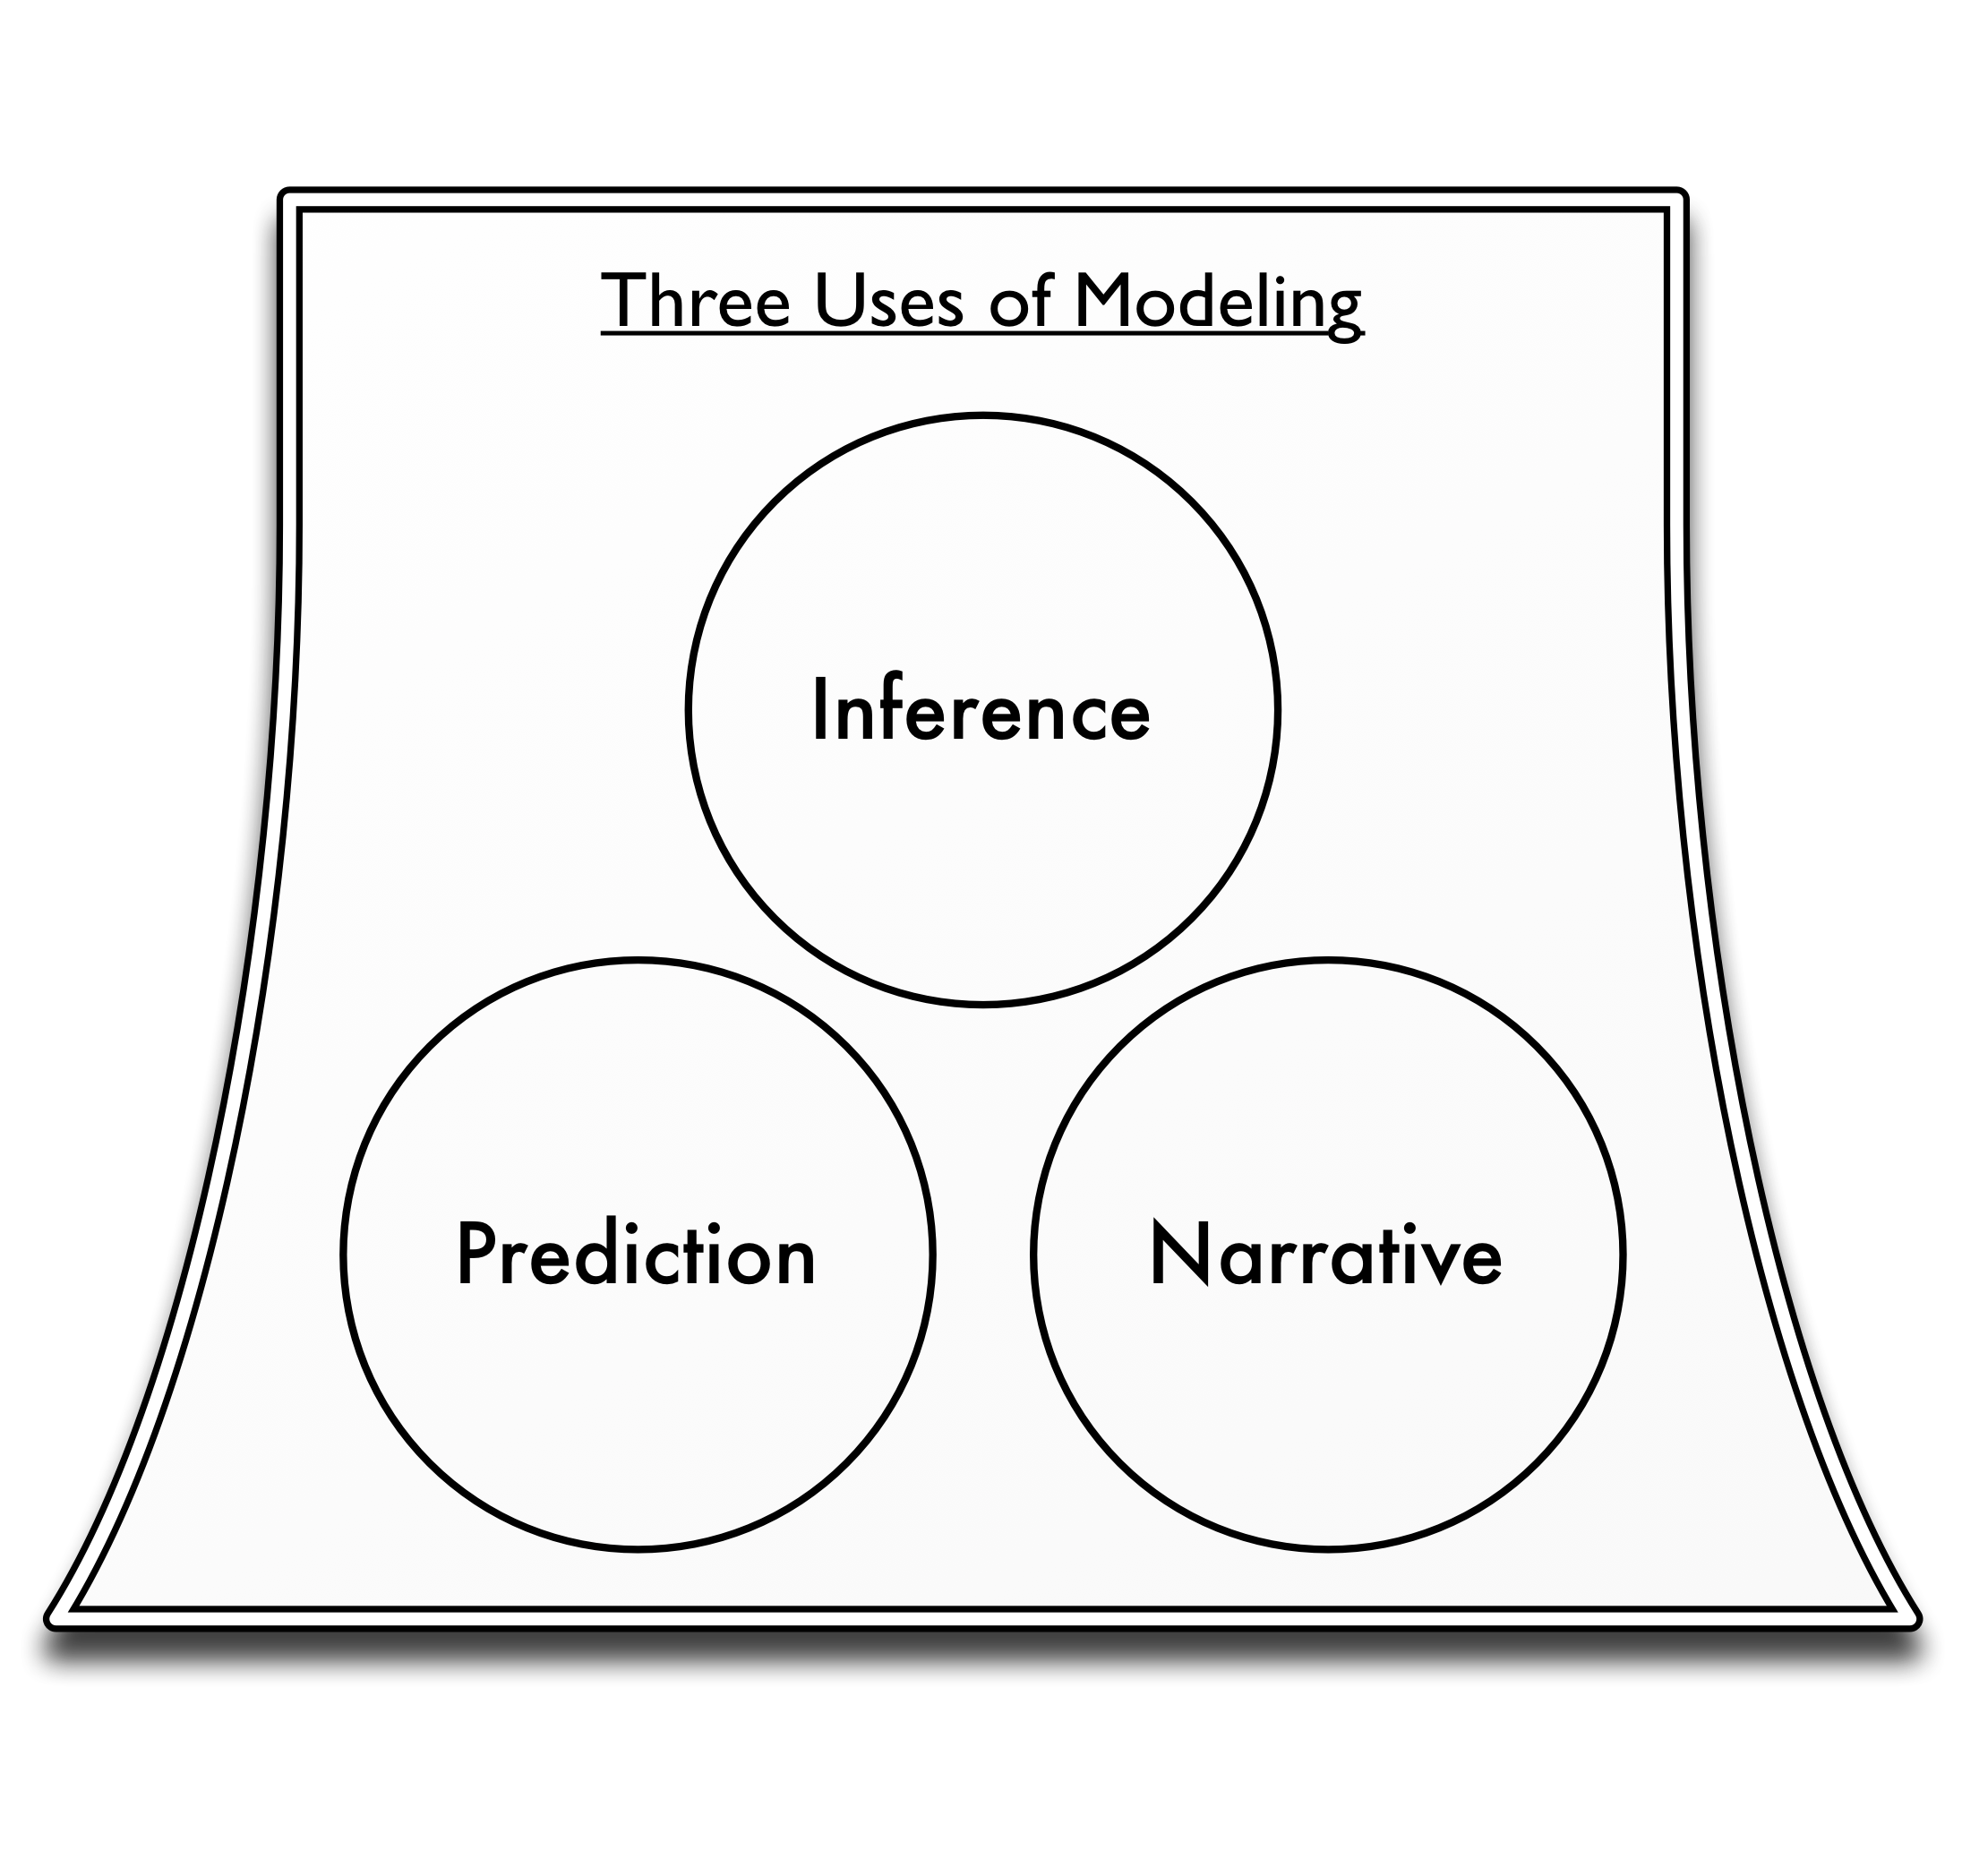
\includegraphics{Usages.png}
\caption{Figure 1. Three Usages of Models}
\end{figure}

Prediction : Models used for prediction are the most straightforward.
They attempt to forecast some outcome given information about variables
that may influence that outcome. A weather forecast is an example of a
model used for prediction. Likewise, when you apply for a credit card at
a bank, they run a predictive model to determine your risk of not paying
them back what you owe and defaulting. When you apply for life
insurance, the company has a model that predicts how long they think you
will live in order to determine how much they should charge you. All
these models take in data (the current temperature for the weather
forecast, the amount of money in your bank account for your risk of
default, your age for the life insurance application) and apply various
forms of analysis to generate a prediction of the outcome.

Inference : Models used for inference are most common in academic
research. Often, academic research questions distills down to this
simple template: ``Does \emph{X} affect \emph{Y}?'' These are
inferential questions\footnote{Predictions are also inferential results,
  but we prefer to discuss prediction and more hypothesis-testing types
  of inference separately. This distinction makes our understanding of
  modeling clearer.}. As an example, a researcher may make a hypothesis
statement such as, ``The wealthier a high-school student's family is,
then the higher the student's test scores will be.'' The researcher may
then build a model to test the validity of this hypothesis and the
model's results will generally be phrased in terms of a \emph{p} value
indicating the statistical significance of the evidence in support of
the hypothesis.

Narrative : Models are often used to tell a persuasive story. When the
Obama administration wanted to persuade lawmakers and the public to
support their economic stimulus, they famously published the graph shown
in Figure 2. A great deal of complex modeling and mathematics surely
went into constructing this figure. However its core purpose was to tell
the nation a story: Things are going to be bad, but the recovery plan
will make them less so. Such stories are at the heart of narrative
models and we will return to this figure later on and why it is not
really a predictive model despite it generating predictions.

\begin{figure}[htbp]
\centering
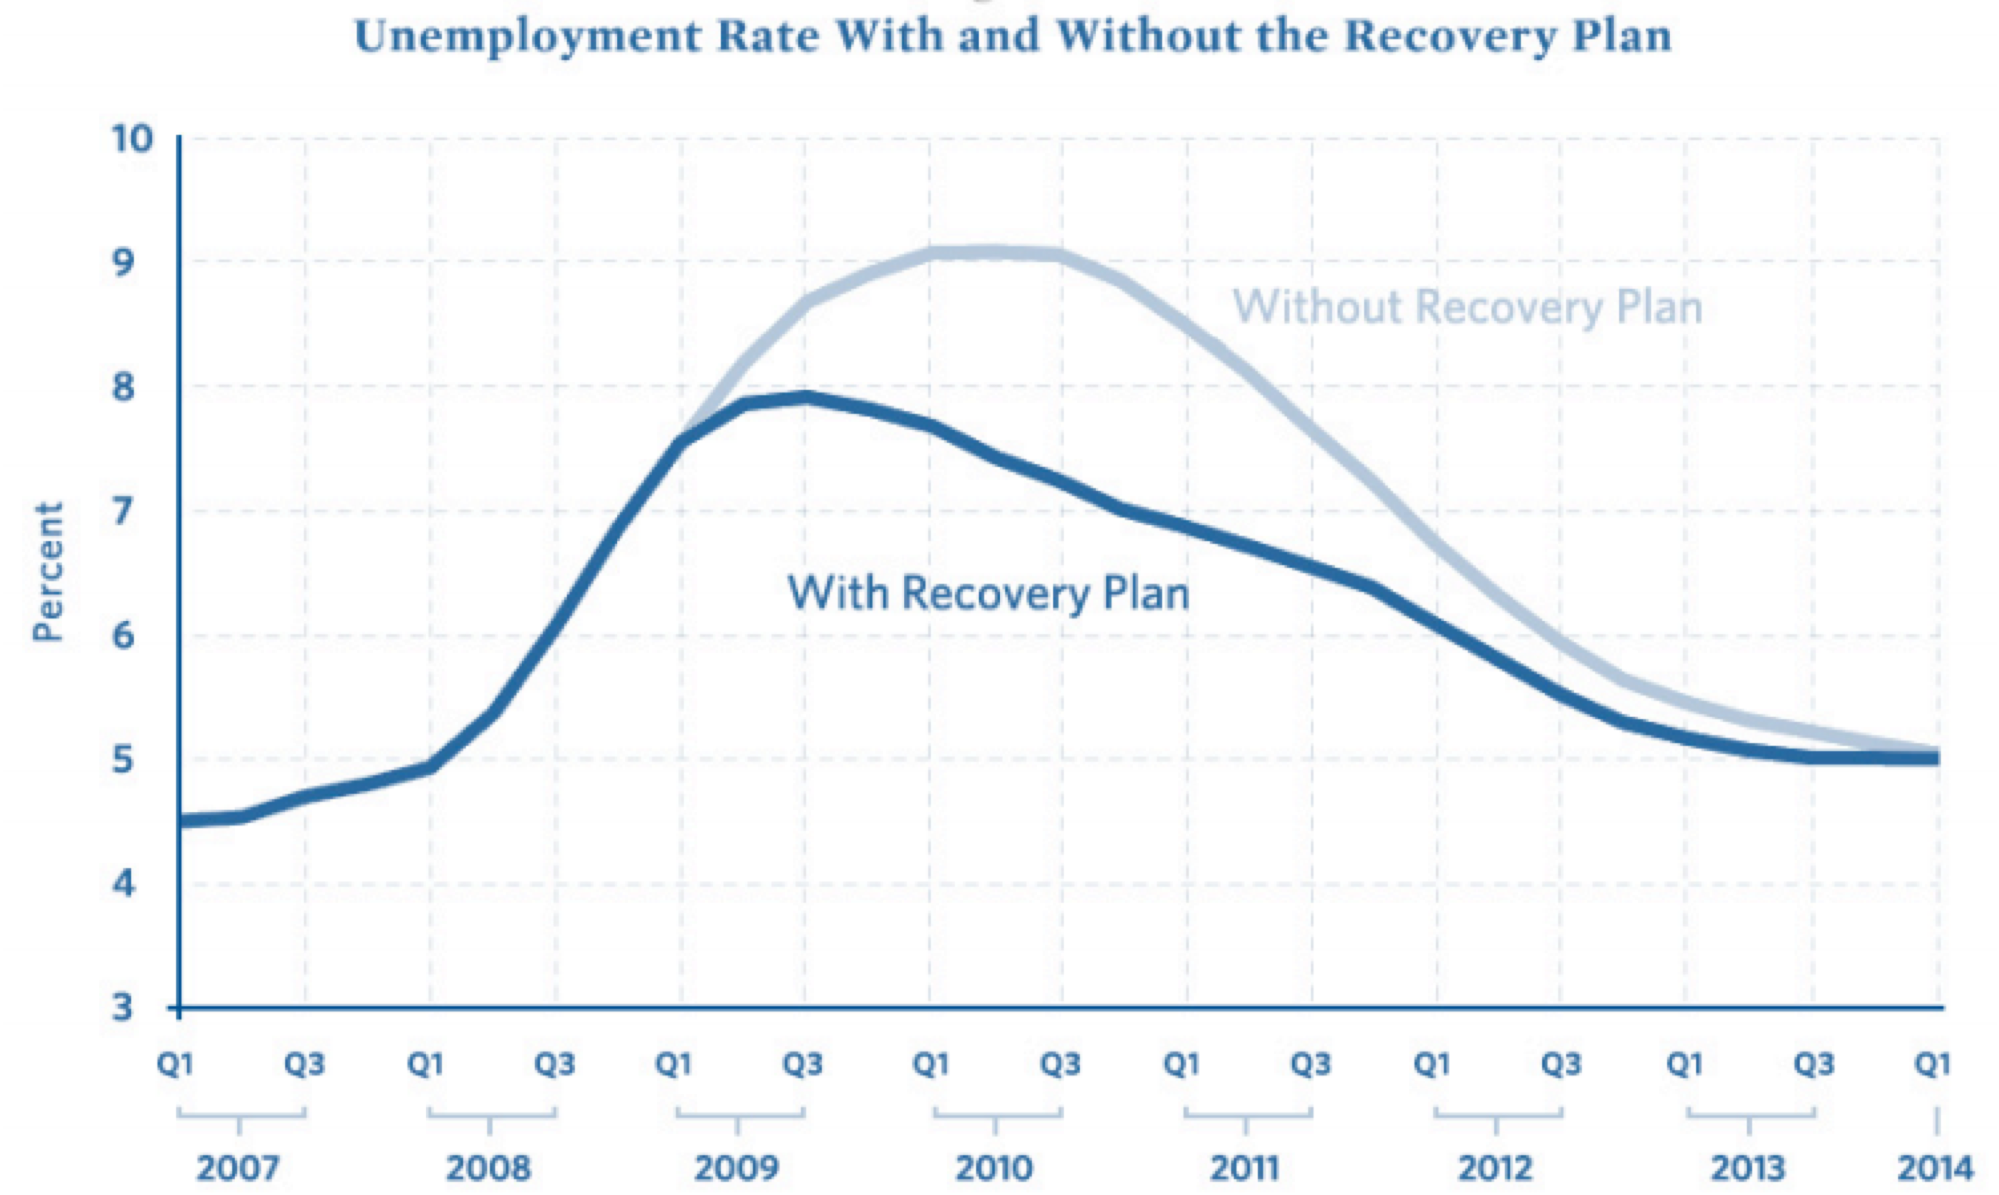
\includegraphics{Stimulus.png}
\caption{Figure 2. The Obama Administration's Predictions for the
Effects of the Recovery Plan (Romer and Bernstein 2009)}
\end{figure}

All models can be classified in terms of these three primary purposes
and we will see how useful it is to discuss modeling projects in terms
of them\footnote{And we strongly recommend doing so. It is important to
  clearly define the purpose at the start of a project. The techniques
  used and data required depend significantly on the model's overall
  purpose. To be very clear, it is important to clarify at the outset
  whether your primary goal is to use a model for prediction or for
  narrative. Many modeling projects may attempt to do both only to find
  themselves with a model that does neither.}.

\hyperdef{}{Ex-8-5}{\paragraph{}\label{Ex-8-5}}

\beginEx{Exercise 8-5}

Classify each of these modeling tasks as either primary prediction,
inference, or narrative tasks:

\begin{enumerate}
\def\labelenumi{\arabic{enumi}.}
\itemsep1pt\parskip0pt\parsep0pt
\item
  A model to determine the average ocean temperature in 2020.
\item
  A model to determine whether deforestation affects temperatures.
\item
  A model to determine whether a company should supply a credit card to
  a specific applicant.
\item
  A model to help students understand the risks of global climate
  change.
\item
  A model to convince your manager to green-light your new initiative.
\item
  A model to assess whether nutrition has an effect of infant mortality.
\end{enumerate}

\hfill{} \hyperref[Ans-8-5]{Answer Available}

\completeEx 

\section{The Strange Case of Inference}

To help us get at this fundamental classification scheme, let's first
talk for a moment about the process of inference. Take the earlier
example of determining whether wealth results in increased high-school
test scores. We phrased this hypothesis in a specific way: that
increased wealth will always increase test scores. This illustrative
statement, however, actually differs from what is often done in
practice. In general, researchers simply asks the question ``Does
\emph{X} affect \emph{Y}?'' rather than ``Does \emph{X} increase
\emph{Y}?'' It's just a slight difference, but it is a more flexible
question that allows for many forms of relationships. For our example,
we would ask the question ``Does wealth affect tests scores?''

The gold standard to answering questions like this is the controlled
experiment. Controlled experiences allow you to develop strong
inferences as you can see how a system responds when you hold all
variables constant except for the single one you are interested in. For
our example, we could imagine an experiment where we took a sample of a
thousand families from a school district. When these families' children
enter high school we would randomly select them to be in a ``poor''
category and the other half to be in a ``rich'' category. Families in
the rich category are given grants of \$500,000 a year to spend how they
wish while the parents in the poor category are fired from their jobs
and have their savings frozen for the duration of the experiment. Once
the students graduate from high school, we would compare the scores for
the students in the poor and rich categories.

These controlled randomized experiments are considered the ideal
approach to answering inferential questions like these as they allow you
to truly determine the effect of your variables, in this case wealth.
For many types of questions, such experiments can be implemented (for
instance does consumption of a new drug help treat a disease).
Unfortunately, in general complex social questions are simply impossible
to answer with them. We can consider the testing procedure we just
imagined to assess the effect of wealth on scores, but it would be
impossible and unethical to undertake in a real community. Furthermore,
even if you were to implement the experiment as described, the behavior
of a family that was poor or wealthy to begin with might very well
differ from a family that experiences a sudden change in income.

\subsection{Traditional Model Based Inference}

Given our general inability to undertake the ideal controlled
experiment, how do we answer inferential questions? The standard way is
to collect data and then construct a model enabling us to measure the
statistical significance of our hypothesis given the data. Due to
history and simplicity, linear regression models are by far the most
commonly used type of model today. A linear regression predicts an
outcome ($Y$) based on the multiplication of variables ($X$'s) by a set
of coefficients determining the effect of the variables on the outcome
($\beta$'s):

\[ Y = \beta_0 + \beta_1 \times X_1 + \beta_2 \times X_2 ... \]

For the education example we could collect data on a number of students,
measuring their families' wealth ($X_1$ in the equation above) and the
student's test scores ($Y$). We would then run the linear regression to
determine the coefficient values ($\beta_0$ -- the intercept -- and
$\beta_1$ -- the effect of wealth on test scores). If we thought there
were other factors that affected test scores, we could measure them and
include them as addition $X$'s in the regression.

In addition to obtaining the values of these coefficients, we also
obtain as a result from the regression the statistical significances or
``\emph{p} values'' of these coefficients. Although \emph{p} values are
commonly used in statistics, they are ubiquitously
misunderstood\footnote{These misunderstandings are not only made by
  on-the-ground practitioners and analysts, they are frequently shared,
  and propagated, by university-level statistics instructors; see, for
  instance, Haller and Krauss (2002).} so it is useful to briefly review
them.

In short a \emph{p} value measures the probability of seeing the
measured data (or more extreme data) assuming the null hypothesis is
true. Generally the null hypothesis will be that there is no
relationship between the variables and the outcomes.

When assessing the significance of coefficients, a \emph{p} value means
the probability of seeing that value of a coefficient (or one even
further from 0), assuming that the (unknown) truth is that the
coefficient actually has a value of 0. In other words, it is the
probability of seeing the observed non-zero value, assuming that the
true value is in fact 0. Frequently, probabilities of 10\%, 5\% or 1\%
or smaller are taken as indicating statistical significance. These low
values indicate that the coefficient value is so far from 0, and the
probability of this occurring by chance so small, that we can reject the
null hypothesis and accept the fact that the coefficient is not 0.

Using the \emph{p} values enables inference by relying on the
statistical significance of the coefficients. If the probability of
$\beta_1$ (the coefficient for the effect of wealth) occurring due to
chance (given it is 0 in reality) is less than, say 5\%, we can claim
with reasonable strength that wealth does in fact affect test scores.
This is the standard approach researchers take to model-based inference
and is used ubiquitously.

\subsection{A Troubled Sea of Assumptions}

Let's stop for a second and consider what we have done here. In carrying
out these logical steps to apply model based inference to determine
whether wealth affects test scores, we have had to make one very large
assumption: that the relationship between test scores and wealth is
linear.

Our linear regression equation assumes that for every increase in one
unit of wealth ($X_1$), test scores ($Y$) will increase on average by
the amount of the coefficient ($\beta_1$). What if this were not in fact
the truth? For instance, we could easily imagine the case where wealth
initially helped test scores by providing students more resources and
opportunities to learn. After a certain point, however, wealth might
negatively impact scores as very wealthy students might lack the
pressure or motivation to study hard.

If we believed this were the case, then our linear regression model from
earlier would be wrong as would the inferences we obtained from the
model. We could correct our model and inferences by changing our
regression formula to contain a squared term that could replicate this
type of relationship:

\[ Score = \beta_0 + \beta_1 \times \text{Wealth} + \beta_2 \times \text{Wealth}^2 \]

Using this equation, at low values of wealth the
$\beta_1 \times \text{Wealth}$ term will have the most effect on scores.
Conversely, at high levels of wealth, the
$\beta_2 \times \text{Wealth}^2$ term will have the most effect on
scores. Thus by having a positive $\beta_1$ and a negative $\beta_2$ we
can model wealth as having an initially beneficial and then detrimental
effect. If our assumptions about the quadratic relationship are correct,
then this model will yield accurate inferences. If they are wrong, our
inferences will be wrong again.

What are we really doing when we assume regression forms like this? Now
it might not be immediately obvious, but what we are in fact doing is
telling a story. Using our first equation, we are telling the story that
as wealth increases test scores will almost always increase. Bill Gate's
children will preform amazingly well here! Using the second equation we
are telling a different story: As wealth increases test scores initially
do as well but after a certain point increased wealth will hurt test
scores. That picture isn't so rosy for the Bill Gates of the world!

And so we arrive at a key insight. By choosing our equations to tell a
story, our inferences are in fact based on narrative modeling
approaches. True, these inferences build upon numerous calculations and
very advanced theoretical underpinnings, but ultimately what governs our
conclusions and inferences are the stories or narratives we tell about
our system. These are choices that we as narrators make and they not
determined by an objective truth or reality.

\paragraph{}

\beginEx{Exercise 8-6}

You are given the following linear regression model that predicts the
growth rate of a tree (in meters per year):

\[
\begin{split}
\text{Growth Rate} = 3.2 + \\
& 0.013 \times \text{Mean Annual Temperature} + \\
& 0.021 \times \text{Annual Precipitation} - \\
& 2.3 \times \text{Moose Density}
\end{split}
\]

Take this mathematical model and convert it to a textual narrative.

\completeEx 

\paragraph{}

\beginEx{Exercise 8-7}

You are given the following linear regression model that predicts the
demand for hats (in thousands of hats sold per day):

\[
\begin{split}
\text{Hat Demand} = 23.4 + 3.4 * \\
& (\text{Temperature in Celsius} - 22)- \\
&1.2 \times \text{Wind Speed} -\\
& 0.21 \times \text{Unemployment Rate}
\end{split}
\]

Take this mathematical model and convert it to a textual narrative.

\completeEx 

\subsection{Predictive Inference}

Is there an alternative approach to inference that does not rely so
heavily on narrative? Can we accomplish it without assuming the
relationships between variables? The answer is yes. Although they are
not often used, alternative prediction-based approaches to inference are
available. In these approaches, rather than calculating statistical
significances as a function of an assumed model, we calculate
significances as a function of the simple question: ``Does knowing
\emph{X} help us to predict \emph{Y}?'' This question is effectively
identical to our earlier question -- ``Does \emph{X} affect \emph{Y}?''
-- but it is structured in an explicitly predictive manner. If the
answer to the question is true, then we can say that there is a
relationship between \emph{X} and \emph{Y}.

The techniques to accomplish prediction-based inference are much newer
than classic techniques as linear regression as they rely upon extensive
computing power and would not be possible without modern technology. One
of these approaches is the \emph{A3} method (XXX Citation) which uses
resampling based algorithms to obtain estimates of predictive accuracy
and statistical significance. \emph{A3} focuses purely on predictive
accuracy of a model to determine whether a variable is significant and
often requires the automatic exploration of hundreds or thousands of
competing models to find the one that best describes the data. The
results of these analyses are inferences that are founded in the data of
model fits only, not on subjective assumptions.

\section{Predictive versus Narrative Modeling}

As we can see, inferential techniques can be split into two categories:
those based on narrative modeling methods and those based on predictive
modeling methods. So -- and this is a key advance -- although there
three categories of model purposes -- prediction, inference, and
narrative -- there are only two fundamental approaches to constructing
models: predictive modeling and narrative modeling.

This divide is not traditionally used in the modeling field, but it is
truly at the heart of modeling. Understanding the distinction between
these two types of modeling proves below to be much more valuable than
mastering fine technical details. The choice of whether to build a
predictive or a narrative model is a fundamental one that shapes every
aspect of a model and determines its ultimate utility for a specific
purpose. The following sections will describe these two types of models
in more detail.

\subsection{Predictive Models}

How do we define a predictive model? The naive answer is that a
predictive model is one that makes predictions. If a model generates
predictions for a future outcome or a given scenario, than it must be a
predictive model. By this definition, a weather forecast is a predictive
model as were the Obama administration's unemployment predictions we saw
earlier.

Unfortunately, this straightforward definition is useless. Worse than
being useless, it is actually quite dangerous.

\begin{center}\rule{3in}{0.4pt}\end{center}

Let us propose a model for next year's unemployment figures in the
United States:

\begin{quote}
Generate a random number from 0 to 1. If the number is less than 0.1,
unemployment will be 20\%. If the number is greater than or equal to
0.1, unemployment will be 0\%.
\end{quote}

There, we have just constructed a model of unemployment. Furthermore,
our model creates predictions. With just a few calculations we can
forecast unemployment for the coming year. Isn't that convenient?

Of course, this model is a joke. It is useless in predicting
unemployment. However, using the naive definition of what it means to a
predictive model, it would be classified as one.

What makes this simple model, such a poor model for prediction purposes?

There are several answers. We might start by saying it is too
\emph{simple}. If we are really trying to predict unemployment we should
incorporate the current economic state and trends into our model. If the
economy is improving, unemployment will probably drop and vice versa.
This is a valid point. Let's address it by proposing an ``improved''
model:

\begin{quote}
Generate a random number from 0 to 1. If the number is less than the
percentage change in GDP over the past year, unemployment will be 20\%
plus the current unemployment rate. If the number is greater than or
equal to 0.1, unemployment will be the net change in the consumer price
index over the past 8 years.
\end{quote}

Is this a better model? Clearly, it is more complex than the previous
one and it incorporates some relevant economic data and indicators.
Equally as clear, however, is that it is also a joke far from being a
useful model.

These toy economic models show that just generating predictions is not a
helpful criterion to define a predictive model. They also show that
complexity and the use of relevant data is not a valid criterion. So how
do we specify a predictive model? The answer is straightforward:

\begin{quote}
A predictive model is a model that not only creates predictions but also
must contain an \emph{accurate assessment of prediction error}.
\end{quote}

Read that statement again. The key point is that the assessment of
prediction error must be accurate, which is different from the accuracy
of the predictions themselves. Of course, ideally the predictions will
be accurate; however this is often not possible. Many systems are
governed to a significant extent by chance and no model, no matter how
good it is, will be able to create accurate predictions for the systems.

If you know the level of prediction error, you can instead contextualize
poorly fitting models. You can determine how much to discount their
predictions in your decision-making and analysis. Furthermore, and this
is crucial, you can compare different predictive models. If your current
model is insufficiently accurate, you can develop another one and
objectively test it to determine whether it is better than the current
model.

Without measures of predictive accuracy, discussing predictions or
comparing models that create predictions is an almost nonsensical
endeavor. Such discussions will be governed by political concerns and
partisanship as there is no objective foundation on which to base them.

Our two proposed models to estimate unemployment are thus clearly not
predictive as no estimate of predictive error has been established. We
can apply same this requirement to Obama's employment predictions we saw
earlier. When we first presented the model, we called it a narrative
model, which might have been slightly perplexing as the model did
generate predictions. However, using our above definition of a
predictive model we can see also that it is in fact not a predictive
model. The model contains no estimate of prediction error (and one is
not available in the original report) so it simply cannot be considered
to be predictive.

If accurate estimates of prediction error are available, you can
directly compare the prediction errors between different models to
select the one with the lowest error. We could estimate prediction
errors for the two joke models we proposed here along with the Obama
administration's model to find the one with the lowest error. We would
hope that the one the Obama administration presented to Congress would
be the most accurate. Before we test it however, we must not make the
error of fallaciously accepting a model to be good based on who
presented it to us or its complexity.

Why do we so rarely hear about the predictive accuracy of models? There
are numerous reasons but they boil down to three basic ones:

\begin{enumerate}
\def\labelenumi{\arabic{enumi}.}
\itemsep1pt\parskip0pt\parsep0pt
\item
  Assessing prediction error accurately is quite difficult.
\item
  Sharing prediction error may perversely decrease an audience's belief
  in a model.
\item
  Most models people use for prediction are in reality narrative models
  and their predictive error is either abysmal or irrelevant.
\end{enumerate}

Let's look at each point in detail. First consider the issue of the
difficulty of assessing prediction error. In general, obtaining an
accurate assessment of prediction error is much more difficult than
developing the predictions themselves. Most commonly used approaches
(for instance the standard $R^2$ from linear regression) have
significant flaws. There are both theoretical and numerical methods that
can be used to make more accurate prediction errors in many cases (this
will be discussed further in the section the
\hyperref[ComplexityCost]{Cost of Complexity}; see also Fortmann-Roe
(2012)). When dealing with time series data, however, like most of the
models explored in this book, it is often almost impossible to
accurately assess model prediction error. Recently, theoretical
technique to approach these issues have just begun to be developed (e.g.
He, Ionides, and King (2009) or A. A. King et al. (2008)) but they are
still impractical to apply in many cases so far.

If the challenge of measuring prediction error is surmounted, there is
an even more formidable barrier to its being published with the model.
There is a perverse phenomena that the act of reporting prediction error
can \emph{decrease} the confidence an audience gives a model. An
anecdote was relayed to us by a member of a team working on a model of
disease spread. His team shared the predictions from the model with a
group of policy-makers. Everything was going fine until the audience saw
the error bars around the predictions. Where his audience had been
content with the raw predictions, they were quite unhappy with the
predictions when accompanied by their accurately estimated
uncertainties. Why was this? Was the team's model particularly bad or
did these policy-makers have a better model at their disposal? No. In a
world where policy-makers and clients are constantly shown models (like
Obama's unemployment figures) with no measure of uncertainty (or even
worse, poorly calculated, artificially low uncertainty), they come to
have unrealistic expectations and often turn away good science in favor
of magical thinking.

Finally, the most likely reason supposedly predictive models do not
include prediction error is that they simply are not predictive. We have
seen how models developed for a purportedly predictive purpose can
actually be narrative models in disguise. Just why is this too often the
case? You need only look at the reason for most modeling projects. It is
very rare that models are commissioned solely for the purpose of
generating an accurate prediction. Frequently, models are part of some
political process within an organization or across them (whether an
organization be a for-profit company or a non-profit such as a
university). Ultimately, the people funding the model expect it to prove
a point to their benefit. In environments like these, it is to be
expected that some predictive modeling efforts will be sidetracked by
political concerns or compromised in the process.

We can see the results of such influences in the predictions generated
for unemployment presented earlier. Figure 3 shows the projections for
the unemployment rates with and without the stimulus plan just as in
Figure 2. Overlaid on this are now the true values of unemployment the
occurred after the predictions were made. As is readily evident, the
original modeling and predictions were well off the mark. Not only was
reality worse than the projections assuming the stimulus was enacted
(which it was) it is much worse than the projections for the economy
assuming the stimulus had never been enacted at all! This is just a
small example -- one that is sadly replicated over and over again in
business and policy-making -- of mistakenly treating a narrative model
as a predictive one.

\begin{figure}[htbp]
\centering
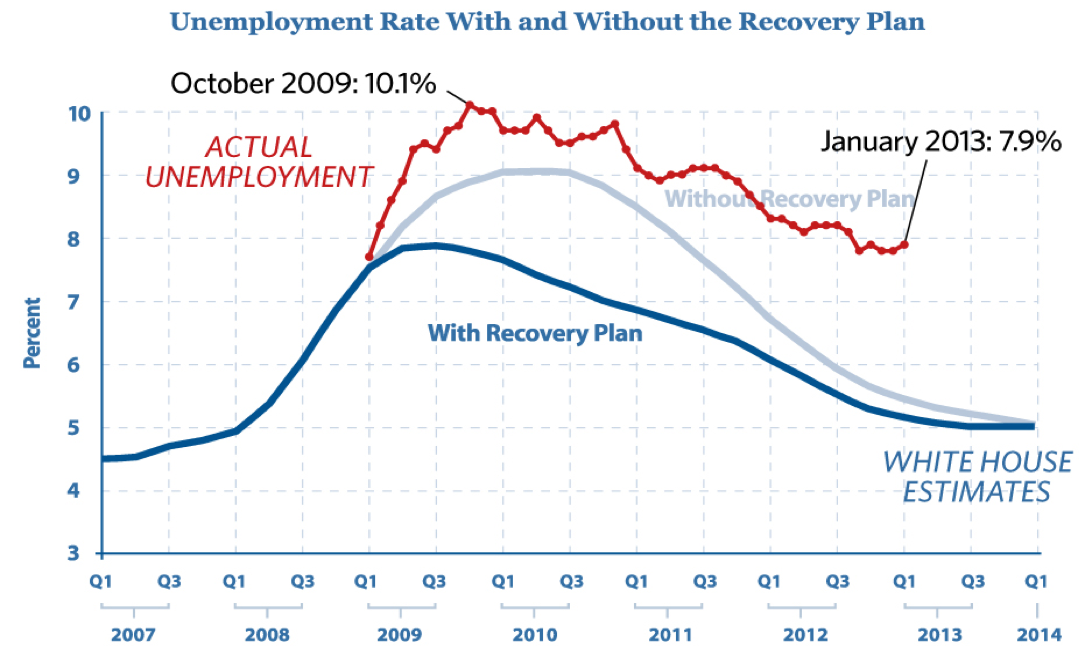
\includegraphics{StimulusAndReality.png}
\caption{Figure 3. Unemployment predictions versus reality (The Heritage
Foundation 2013)}
\end{figure}

\subsection{Narrative Models}

In contrast to predictive models, a narrative model is one built to
persuade and transform an audience's mental models by telling a story.
When many people first hear the ``narrative'' terminology, they respond
negatively. ``It's just a story.'' We find this strange, as narratives
are the fundamental human form of communication. We tell narratives to
our friends and relatives. Politicians communicate their policies to us
using narratives. Of course the vast majority of our entertainment is
focused on narratives\footnote{Even sports, a form of entertainment that
  innately contains no narrative, becomes wrapped in narrative as the
  announcers and commentators attempt to create stories to engage us.}.
Business leaders and managers attempt to describe their strategies to us
using story lines; and business books are in general dominated by
anecdotes plotted along the way to making their points.

We as a species do not view the world as a collection of numbers and
probabilities; instead we see consequence and meaning. In short,
narratives are how we see the world.

One critique of the term narrative is that it lacks numbers, quantified
data, or mathematics. This could not be further off the mark. There are
many ways to construct narratives. Words are one, pictures are another,
and music is a third. Numbers and mathematics are just another way of
telling a story.

In fact, most statistical and mathematical models are infused with
narrative models. We looked earlier at the case of linear regression as
a tool to predict test scores as a function of wealth. Again the
mathematical equation for this simple model was:

\[ Score = \beta_0 + \beta_1 \times Wealth \]

This equation defines a narrative. Translating this narrative into
words, we would say:

\begin{quote}
Test scores are only determined by the wealth of a student's family. A
child whose family is broke will have a test score, on average, of
$\beta_0$. For every dollar of wealth a child's family accumulates, the
child will score, on average, better on tests by $\beta_1$.
\end{quote}

You might or might not agree with this storyline (in our view it is a
nonsensical and reductionist view of child achievement) but it shows the
strict equivalence between this mathematical narrative and narrative
prose. This process can be applied to all mathematical models. The
mathematical definition of the model can be converted directly, with
more or less lucidity, into a story describing how the system operates.
The same can also be done in the reverse: we can take a descriptive
narrative of a system and convert it into a mathematical description. As
we have seen (will see? XXX) this is what tools like reference modes and
pattern matching are designed to do efficiently: elicit a narrative from
a subject in a way which can be reformulated quantitatively.

The question of how to assess the quality of a narrative model is an
important one. With predictive models, we can compare competing models
based primarily on predictive accuracy\footnote{Other criteria include
  ease of use, cost of filling data requirements, and computational
  requirements. But all those are generally secondary to prediction
  accuracy.}. But how do we evaluate and compare the quality of
narrative models?

The key criterion in assessing a narrative model is its ability to be
\emph{persuasive}. Although persuasion is not an objective measure in
the same sense prediction accuracy is, we can decompose persuasiveness
into two components for our purposes: believability and clarity. A
persuasive model is one that is both believable and effectively
communicates its message.

When building a narrative it is very important to use tools that are
well suited to meeting these components. Unfortunately, many statistical
models, including regressions, are poorly suited to this two-fold task
in many ways. Most statistical models depend on unrealistic and highly
technical assumptions about the data. If these assumptions were
enumerated in plain English, they would often conflict with people's
understanding and in fact end up discrediting the model. The
``alternative'' has been to leave these assumptions hidden creating a
black box model opaque to outside inspection.

This is a shame in our view. Such a stratagem can be successful if the
authority presenting the model is prestigious enough. But the
misdirection will quickly fail if any kind of rigorous scrutiny is
applied to the model. Narrative models should never be given any real
credence if the operation of the model is not transparent. Most
statistical models are built on assumptions that are never made
transparent to the audience.

The modeling techniques presented in this book, on the other hand, are
well suited for narrative modeling. The techniques we present are
``clear box'' modeling where the workings of the model are transparently
evident and accessible. Our models have their structure explicitly
described using an accessible modeling diagram showing the interactions
between the different components in the model. The equations governing
the model's evolution are clear and readily available for each part of
the model\footnote{Admittedly, for complex models it may still require a
  significant investment on the part of an audience to fully understand
  the logic and equations in the model. But the opportunity is
  available.}. Furthermore, these modeling techniques used here make it
straightforward to generate animated illustrations and displays to
clearly communicate model results.

\paragraph{}

\beginEx{Exercise 8-8}

Summarize the distinction between predictive and narrative models.

\completeEx 

\section{Synthesis}

Now that we have thoroughly described the concepts of narrative and
predictive models we can conclude this chapter by taking a step back and
reemphasizing that these two categories do to represent specific
modeling techniques. You can build a stock and flow model to tell a
story about a system resulting in a narrative model. If your story of
the system accurately represents how the system operates in reality,
then you will also have a model that generates accurate predictions.

Similarly, you can apply a linear regression to a dataset. If the
relationship in the data is truly a completely linear one, then the
result of this regression will be the most accurate predictive model you
could build. On the other hand, if you do not assess the predictive
accuracy of the model and just use a linear regression because it is
easy to interpret or because it matches you understanding of reality,
then you have a narrative model.

The key criteria to remember when building your own models or assessing
other peoples models is that a predictive model is one for which you
have an accurate assessment of the errors of the predictions. A good
predictive model is one that has low relative errors when compared to
other predictive models for the same system. A narrative model is one
that tells a story about the system. A good narrative model is one that
persuades an audience and by persuading, the model transforms the mental
models of its audience.

\chapter{Building Confidence in Models}

When used correctly, the transparency of the modeling techniques
presented in this book results in models that are powerful persuasive
tools. As with any model, however, there are concerns and questions will
invariably be raised which could cause users to doubt the result of the
modeling work. There are a number of techniques that you can use to help
preemptively address these concerns and increase an audience's
confidence in your model.

The idea of building confidence in a model is closely tied to the
standard concept of model verification and validation. We dislike this
conceptual approach to assessing models as it seems to imply that a
model can go through a process to get a big fat ``VALID'' or
``VERIFIED'' stamp on it. Returning to Box's quote that ``all models are
wrong, but some are useful'', in reality all models are wrong and none
of them are completely valid, period. Models can however be useful,
especially narrative models in which the audience has confidence.

We favor the conceptual approach put forth by Forrester and Senge
(1978), that there is not any single test or suite of tests that will
verify or validate a model and that validity should instead be thought
of as a function of confidence. This is a view that differs from that
held by some modelers and laypeople. As Forrester and Senge note, ``the
notion of validity as equivalent to confidence conflicts with the view
many seem to hold which equates validity with absolute truth.'' We share
their belief that model confidence is built up piece by piece from a
variety of tests that, though they cannot prove anything, together
comprise a persuasive case for the quality of a model.

There are three distinct areas where confidence needs to be developed:

\begin{enumerate}
\def\labelenumi{\arabic{enumi}.}
\itemsep1pt\parskip0pt\parsep0pt
\item
  That the model itself is well designed.
\item
  Given a design of the model, this design is implemented correctly.
\item
  The conclusions drawn from the model are accurate.
\end{enumerate}

In the remaining sections of this chapter we will look at each of these
different areas in detail. We will explore the different tests and tools
that can be used to build confidence for each area.

\section{Model Design}

Fundamentally the design of a narrative model is of utmost importance
and needs to be justified to an audience\footnote{This is different from
  predictive models where the results of the model are much more
  important than the design and the ``proof is in the pudding''" so to
  speak.}. There are two primary aspects to a model's design design: the
structure of the model and the data used to parameterize the model.

\subsection{Structure}

The structure of the model should mirror the structure of the system
being simulated. Depending on the system complexity, the model structure
may need to carry out more or less aggregation and simplification of
this reality. Nevertheless, all the primitives in the model should map
on to reality in a way that is understandable and relatable to the
audience. Thus if there is some object in the real system that behaves
as a stock, a stock should exist in the model mirroring the object's
position within the system. The same should hold true with the other
primitives in the model. Each primitive would ideally be directly
mappable onto a counterpart in the real system and any key component in
the real system should be mappable onto primitives in the model.
Furthermore, feedback loops that exist in the system should exist within
the model. These feedback loops should be explicitly identifiable in the
model and would ideally be called out or marked in a way that
highlighted their presence to an audience.

Furthermore, the model structure should include components that an
audience thinks are important drivers of the system. Missing a factor
that the audience considers to be a key driver can fatally discredit a
model in an audience's mind irrespective of the performance or other
qualities of a the model. This is true even if the factor has in fact a
negligible effect. Generally speaking, it is much easier to include a
factor an audience views as important than it is to later on convince
the audience that the factor does not in actuality matter.

\subsection{Data}

The more a model uses real-world data, the more confidence an audience
will have in the model. Ideally, you have empirical data to justify the
value of every primitive in your model. In practice, such a goal may be
a pipe dream. Indeed, for a complex model, obtaining data to
parameterize every aspect of it is usually impossible\footnote{Leading
  to the clichéd conclusion of many modeling studies: ``We are unable to
  draw strong conclusions from this modeling work. Instead, our
  contribution has been to show where additional data needs to be
  collected.''}. When faced with model primitives that do not have
empirical data to parameterize them, an approach must be taken to ensure
that it does not appear that their values were chosen without
justification or to arrive at a predetermined modeling conclusion.
Sensitivity testing, as discussed later on, is one way to achieve this.
Another is to carry out a survey of experts in the field in order to
solicit a set of recommended parameter values that can then be
aggregated or used to justify the ultimate parameterization.

\subsection{Peer-Review}

Going through a peer-review process can be extremely useful in
establishing confidence in a model. Two general types of peer-review are
available. In one, the model may be incorporated into an academic
journal article and submitted for publication. The article will then
peer-reviewed by generally two or three anonymous academics in the field
who critique it and judge whether or not it is a worthy contribution to
the literature, thus meriting publication. In the second type of
peer-review, a peer-review committee may be assembled (hired) to review
a specific model and provide conclusions and recommendations to clients.

Peer-review can be very useful in establishing the credibility of a
model. A credible model is a model one can be more confident in, other
things being equal. By engaging an independent group of exports to
assess the model, their conclusions about its quality have the
appearance of greater validity than those of the self-interested
modelers\footnote{When the peer review panel is hired by the client
  there is some conflict of interests, but the panel members should not
  be swayed by this.}. This can be especially useful when trying to meet
some abstract standard such as that the model represents the ``best
available technology'' or the ``best available science''.

A key risk of a peer-review is, of course, that the peer-review members
will find a model deficient in important respects. Good criticism can be
very useful and help improve a model. However, some criticism received
in practice may be nitpicking details or detrimental advice that would
make the model worse if followed.

\section{Model Implementation}

Although it is not as much a lightning rod as is model design, the
implementation of a model specification is a point where significant
error can occur. Programming mistakes or mistyped equations can
introduce bugs into a model that can be hard to identify later on. This
is a particular problem in black-box models but it is still an important
point to consider for all types of models including those presented in
this book. Fortunately, a number of steps can be taken to ensure the
model is implemented correctly.

\subsection{Primitive Constraints}

For many of the primitives in the model, there will be natural
constraints. For instance, a stock representing the volume of water in a
lake can never fall below 0. Similarly, if a variable represents the
probability of an event occurring, it must be between 0 and 1.

Often these constraints are implicit without being formally specified in
the model. A modeler may think, water volume can never become negative
so why would I need to specify it? However, the existence of these
constraints provides an opportunity to implement a level of automatic
model checking. By specifying that a primitive can never go above or
below a value (using the \a{Max Value} and \a{Min Value} properties in
Insight Maker), you can create in effect a canary in the coal mine that
warns if something is wrong in the model. If these constraints are
violated an error message can be given letting you know that you need to
correct some aspect of your model.

This concept of constraints in models is similar to the concept of
``contracts'' which are support in some programming languages. These
contracts define and constrain the interaction between different parts
of the program causing an error to be generated if the contract is
violated. The Eiffel programming language probably has the best support
for this approach to development.

\subsection{Unit Specification}

Since we introduced units in Chapter 3, we showed that they could be a
useful tool in constructing models. Units can also be used to ensure
that equations are entered correctly. If you fully specify the units in
a model, many types of equation errors will result in invalid units,
which will create an immediate error. By employing units in your model
you can automatically catch a whole class of errors and mistyped
equations.

\subsection{Regression Tests}

Other tests than those specified above can be developed. For instance,
the proper behavior of one part of the model may be determined and
automated tests created to periodically confirm that the model continues
to exhibit the correct behavior. Development of such tests are a common
part of software engineering that we wish would see more use in model
development. Insight Maker itself has a suite of over 1,000 individual
regression tests that automatically test every aspect of its simulation
engine.

In regards to regression testing, it is important to ensure these tests
are automated. It is not enough to examine a portion of the model,
determine it is currently working correctly, and leave it at that. The
problem is that future changes may break the existing functionality
(i.e.~a ``regression'', the introduction of an error or reduced quality
compared to an earlier version of the model). Especially for complex
models, a change in one part of the model may have an unexpected effect
in another part. By implementing a set of automatic checks, you can
protect your model against unintended changes and regressions.

George Oster and his class XXX

\hyperdef{}{Ex-9-1}{\paragraph{}\label{Ex-9-1}}

\beginEx{Exercise 9-1}

You have a variable representing the total population size of a small
city. What constraints might you place on this variable?

\hfill{} \hyperref[Ans-9-1]{Answer Available}

\completeEx 

\subsection{A Second Pair of Eyes}

That is not to say, however, that spot and point-in-time checks are not
worthwhile. It can be very useful to have a second modeler review your
models and cross-check the equations. This helps not only to check
simple mistakes but also to question and critique the fundamental
structure and choices of the model.

The gold standard in verifying that a model is implemented correctly
according to specification is to have a second modeler completely
reimplement the model according to that specification. Such
reimplementation should ideally occur without access to the original
model's code base to ensure that the second modeler does not simply copy
bugs from the original model into the reimplementation. If the results
from the two implementations concur, that is strong evidence that the
model has been implemented correctly. Although potentially an expensive
exercise, it will also most likely identify numerous ambiguities in the
specification, which could be valuable in and of itself.

\section{Model Results}

Given that the design of the model and its implementation are assumed to
be correct, the burden still falls upon the modeler to transfer her
confidence in the model's results to her audience. There are several
different ways this can be done.

\subsection{Expected Results}

The first way is to demonstrate that the model generates expected
results for normal inputs. For instance, if you had a model a reservoir,
you would expect the volume of the reservoir to decline over time during
the summer due to evaporation if no more water flowed into it. You can
additionally test extreme scenarios and show that they generate the
expected results. If, for example, your reservoir were empty, you would
expect the amount of water evaporating from it to be zero. By
enumerating these standard cases and showing the model results match the
expected results you can help build confidence in the model.

Often these expected results can be described in terms of a curve
showing how the values of one of the stocks or variables in the system
is expected to change over time. This curve can be taken from historical
data (a reference behavior pattern), or simply drawn on a piece of paper
by experts familiar with the system (an excepted behavior pattern).

\subsection{Counterintuitive Results}

Another attempt to increase confidence in a model is to show unexpected
results that are justifiable. Imagine a model that for a certain set of
inputs would create what, at first glance, appeared to be the ``wrong''
behavior. Some lever in the model could lead to unexpected results. When
first shown these results, they could decrease an audience's confidence
in the model. If the audience was then walked through the model step by
step to show how those results proved to be correct and mirrored
reality, then that could well increase their confidence in the model
results.

\subsection{Forecasting}

Possibly the most persuasive action to convince an audience of the
effectiveness of a model is to forecast the future and then to show this
forecast to be correct. This, of course, is difficult to do in practice
for multiple reasons including the fact that the scale of a model is
often such that it could take several years or decades to generate data
to test the model. Additionally, it must be remembered that most
narrative models are poor predictors and should not be used for
predictive purposes solely.

\subsection{Sensitivity Testing}

Sensitivity testing is a broad field that has the potential to address
many questions and doubts that may arise about a model. In general, the
variables and numeric configuration values in a model will never be
known with complete certainty. When the results from an election poll
are published, the pollsters publish not only their predictions but also
the uncertainty in the prediction (e.g., ``the Democratic candidate will
obtain $52\% \pm 3\%$ of the vote''). Similarly when a building is
constructed, the materials used will have certain properties -- such as
strength -- that again are only known up to some errors or tolerance. It
is the engineer's and contractor's responsibilities to ensure that the
materials are sufficient even given the uncertainty of their exact
strengths.

The same occurs when modeling. Most primitive values in the model will
have to be estimated by the modeler and there will be an error
associated with these values. Of course the error will also be
propagated through the model when it is simulated and affect the results
generated by the model. This error is one factor that can create doubt
about a model and reduce an audience's confidence.

As a modeler, one approach to address this doubt would be to try to
measure all the model's variables with great accuracy. You could search
the available literature, undertake a meta-analysis of current results,
carry out new experiments, and survey experts to get as precise a set of
parameter values as possible. If you were able to say with strong
certainty that these values were so accurate and the errors so small
that their effect on the results in negligible, then that would be one
way of addressing the issue of uncertainty.

However, all of this is often impossible to do. When dealing with
complex systems it is almost always the case that at least a couple
variable values will never be known fully with certainty. In this case,
no matter how much research or experiments you do, you will never be
able to pin down the precise values of these variables. How do we handle
these cases?

The answer is straightforward: Rather than trying to eliminate the
uncertainty, we embrace it by explicitly including it in the model. If
you can then show that the results of your model do not significantly
change even given the uncertainty, you have a persuasive case for the
validity of your results. Of course the results will always change when
the uncertainty is introduced, but if the model conclusions persist even
in the face of this uncertainty it will greatly increase your audience's
confidence in the results.

Uncertainty can be explicitly integrated into a model by replacing
constant primitive values with a construct that represents the
uncertainty in that value. Imagine you had a simple population model of
rabbits in a cage. You want to know how many rabbits you will have after
two years. However, you don't know how many rabbits there initially are
in the cage. You have been told that there are probably 12 rabbits, but
the true number could range anywhere from 6 to 18.

If you model your population as a single stock, what should the initial
value be? A naive model could be built where you the initial value of
the rabbit stock was specified as 12. However, that does not incorporate
the uncertainty and could be a source of criticism or doubt for the
model. An alternative would be to specify that the initial value of the
stock is a random number with a minimum value of 6 and a maximum value
of 18. So each time you run the model you will get a different result.
If you ran the model once, the initial value might be chosen to be 7 and
you would obtain one result. If you ran the model again, the initial
value might be 13 and you would get another result.

If you run this stochastic model many times, you obtain a range of
results. These results can be automatically aggregated to show the range
of outputs. For instance if you ran the model 100 times you could see
what the maximum and minimum final populations were. This would give you
a good feeling for how many rabbits you needed to prepare for after two
years. In addition to the maximum and minimum you might be interested in
the average of these 100 runs: the expected number of rabbits you would
see. You could also plot the distribution of the final population sizes
using a histogram to see how the results are distributed. This
distribution would show how sensitive the outputs are to the uncertainty
in the inputs: a form of sensitivity testing.

\begin{figure}[htbp]
\centering
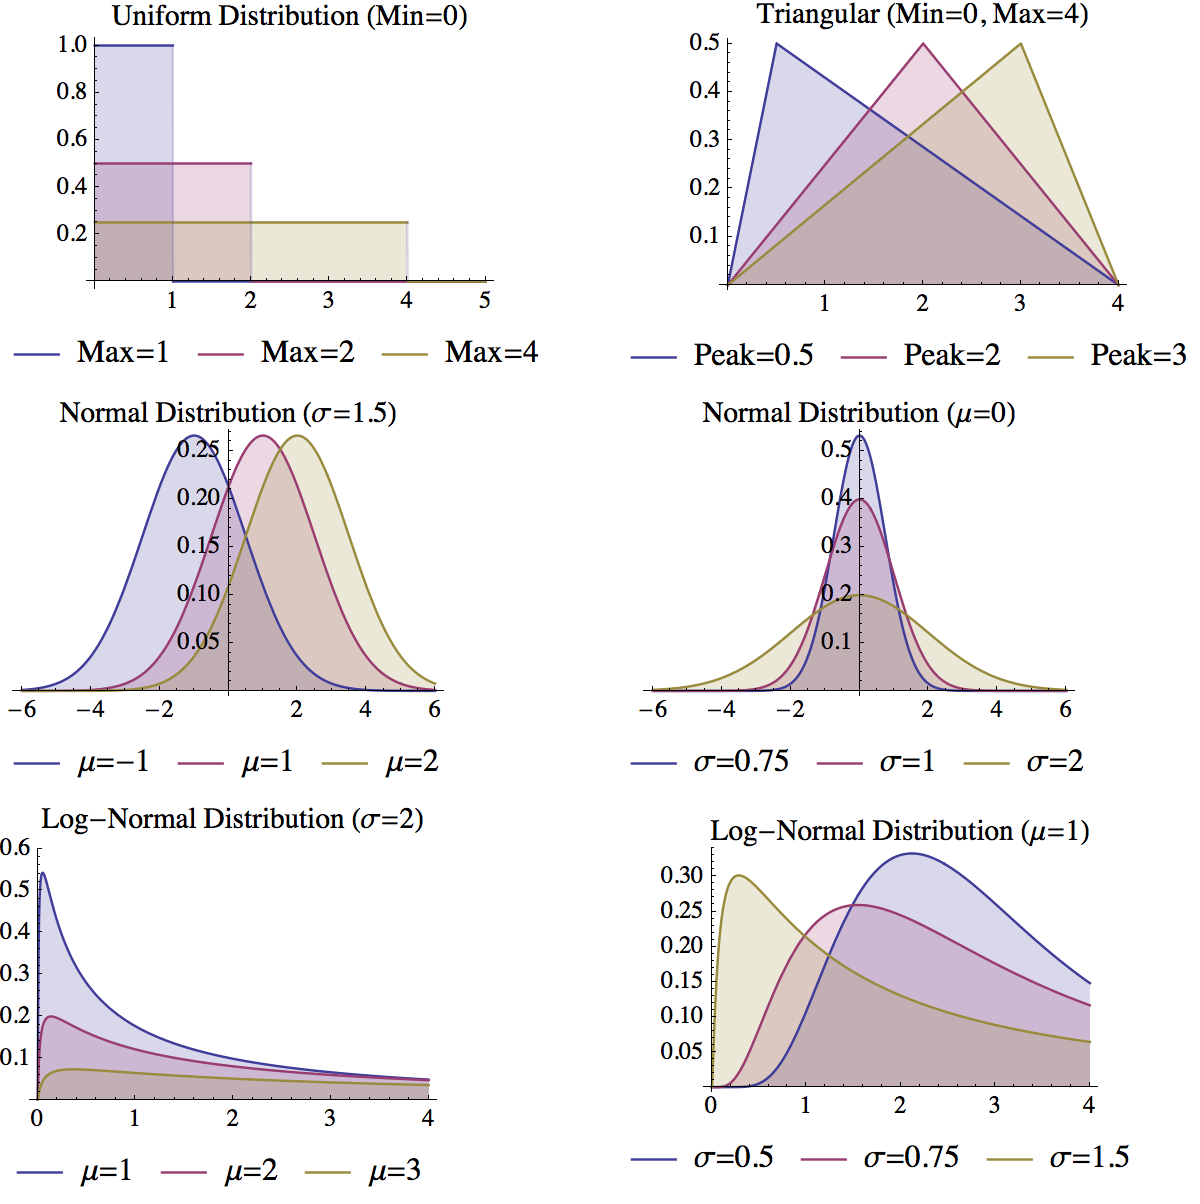
\includegraphics{Distributions.png}
\caption{Figure 1. Common Distributions for Sensitivity Testing with
Sample Parameter Values}
\end{figure}

There are four key distributions that are useful for specifying the
uncertainty in a variable:

Uniform Distribution : The uniform distribution is defined by two
parameters: a minimum and a maximum. Each number within these two
boundaries has an equal probability of being sampled. The uniform
distribution is useful when you know the boundaries on the values a
variable can take on, but you do not have any information on the
likelihood of the different values within this region. The uniform
distribution can be used in Insight Maker using the function
\lstinline!Rand(Minimum, Maximum)!, the two parameters are optional and
will default to 0 and 1 if \lstinline!Rand()! is called without them.

Triangular Distribution : The triangular distribution is defined by
three parameters: the minimum, the maximum, and the peak. Like the
uniform distribution, the triangular distribution will only generate
numbers between the minimum and maximum. Unlike the uniform
distribution, the triangular distribution will not sample all numbers
between these boundaries with equal likelihood. The value specified by
the peak will have the most likelihood of being sampled with the
likelihood falling off as you move away from the peak towards either the
minimum or maximum boundary. The triangular distribution is useful when
you know the both the most likely value for a variable and you also know
boundaries for the values a variable can take on. The triangular
distribution can be used in Insight Maker using the function
\lstinline!RandTriangular(Minimum, Maximum, Peak)!.

Normal Distribution : The normal distribution is defined by two
parameters: the mean of the distribution (generally denoted $\mu$) and
the standard deviation of the distribution (generally denoted $\sigma$).
The most likely value to be sampled from the normal distribution is the
mean. As you move away from the mean (in either a positive or negative
direction), the likelihood of a number being sampled decreases. The
standard deviation controls how fast this likelihood falls as you move
away from the mean. Small standard deviations result in steep declines
in the likelihood while large standard deviations result in more gradual
declines. The normal distribution is useful when you do not have
boundaries on the values for a variable but you do know what the most
likely value for the variable should be (the mean). The normal
distribution can be used in Insight Maker using the function
\lstinline!RandNormal(Mean, Standard Deviation)!.

Log-normal Distribution : The log-normal distribution is closely related
to the normal distribution. In fact the logarithm of the values samples
from a normal distribution will be log-normally distributed. Like the
normal distribution, the log-normal distribution is defined by two
parameters: the mean and standard deviation. Where the log-normal
distribution differs from the normal distribution, is that negative
values will never be generated by the log-normal distribution. Thus it
is useful when you have a variable which you know cannot be negative but
for which you do not have an upper bound. The log-normal distribution
can be used in Insight Maker using the function
\lstinline!RandLogNormal(Mean, Standard Deviation)!. The log-normal
distribution can also be used to represent other types of one-sided
boundaries. For instance, the following equation could be used to
represent a variable whose number was always less than 5:
\lstinline!5-RandLogNormal(2, 1)!

There are many other forms of probability distributions. Some notable
ones are the Binomial Distribution
(\lstinline!RandBinomial(Count, Probability)!), the Negative Binomial
Distribution (\lstinline!RandNegativeBinomial(Successes, Probability)!),
the Poisson Distribution (\lstinline!RandPoisson(Lambda)!), the
Exponential Distribution (\lstinline!RandExp(Lambda)!) and the Gamma
Distribution (\lstinline!RandGamma(Alpha, Beta)!). These distributions
can be used to address very specific modeling usage cases and needs (for
instance, the Poisson distribution can be used to model the number of
arrivals over time), however, the four distributions described in detail
above should generally be sufficient for most sensitivity testing needs.

\begin{figure}[htbp]
\centering
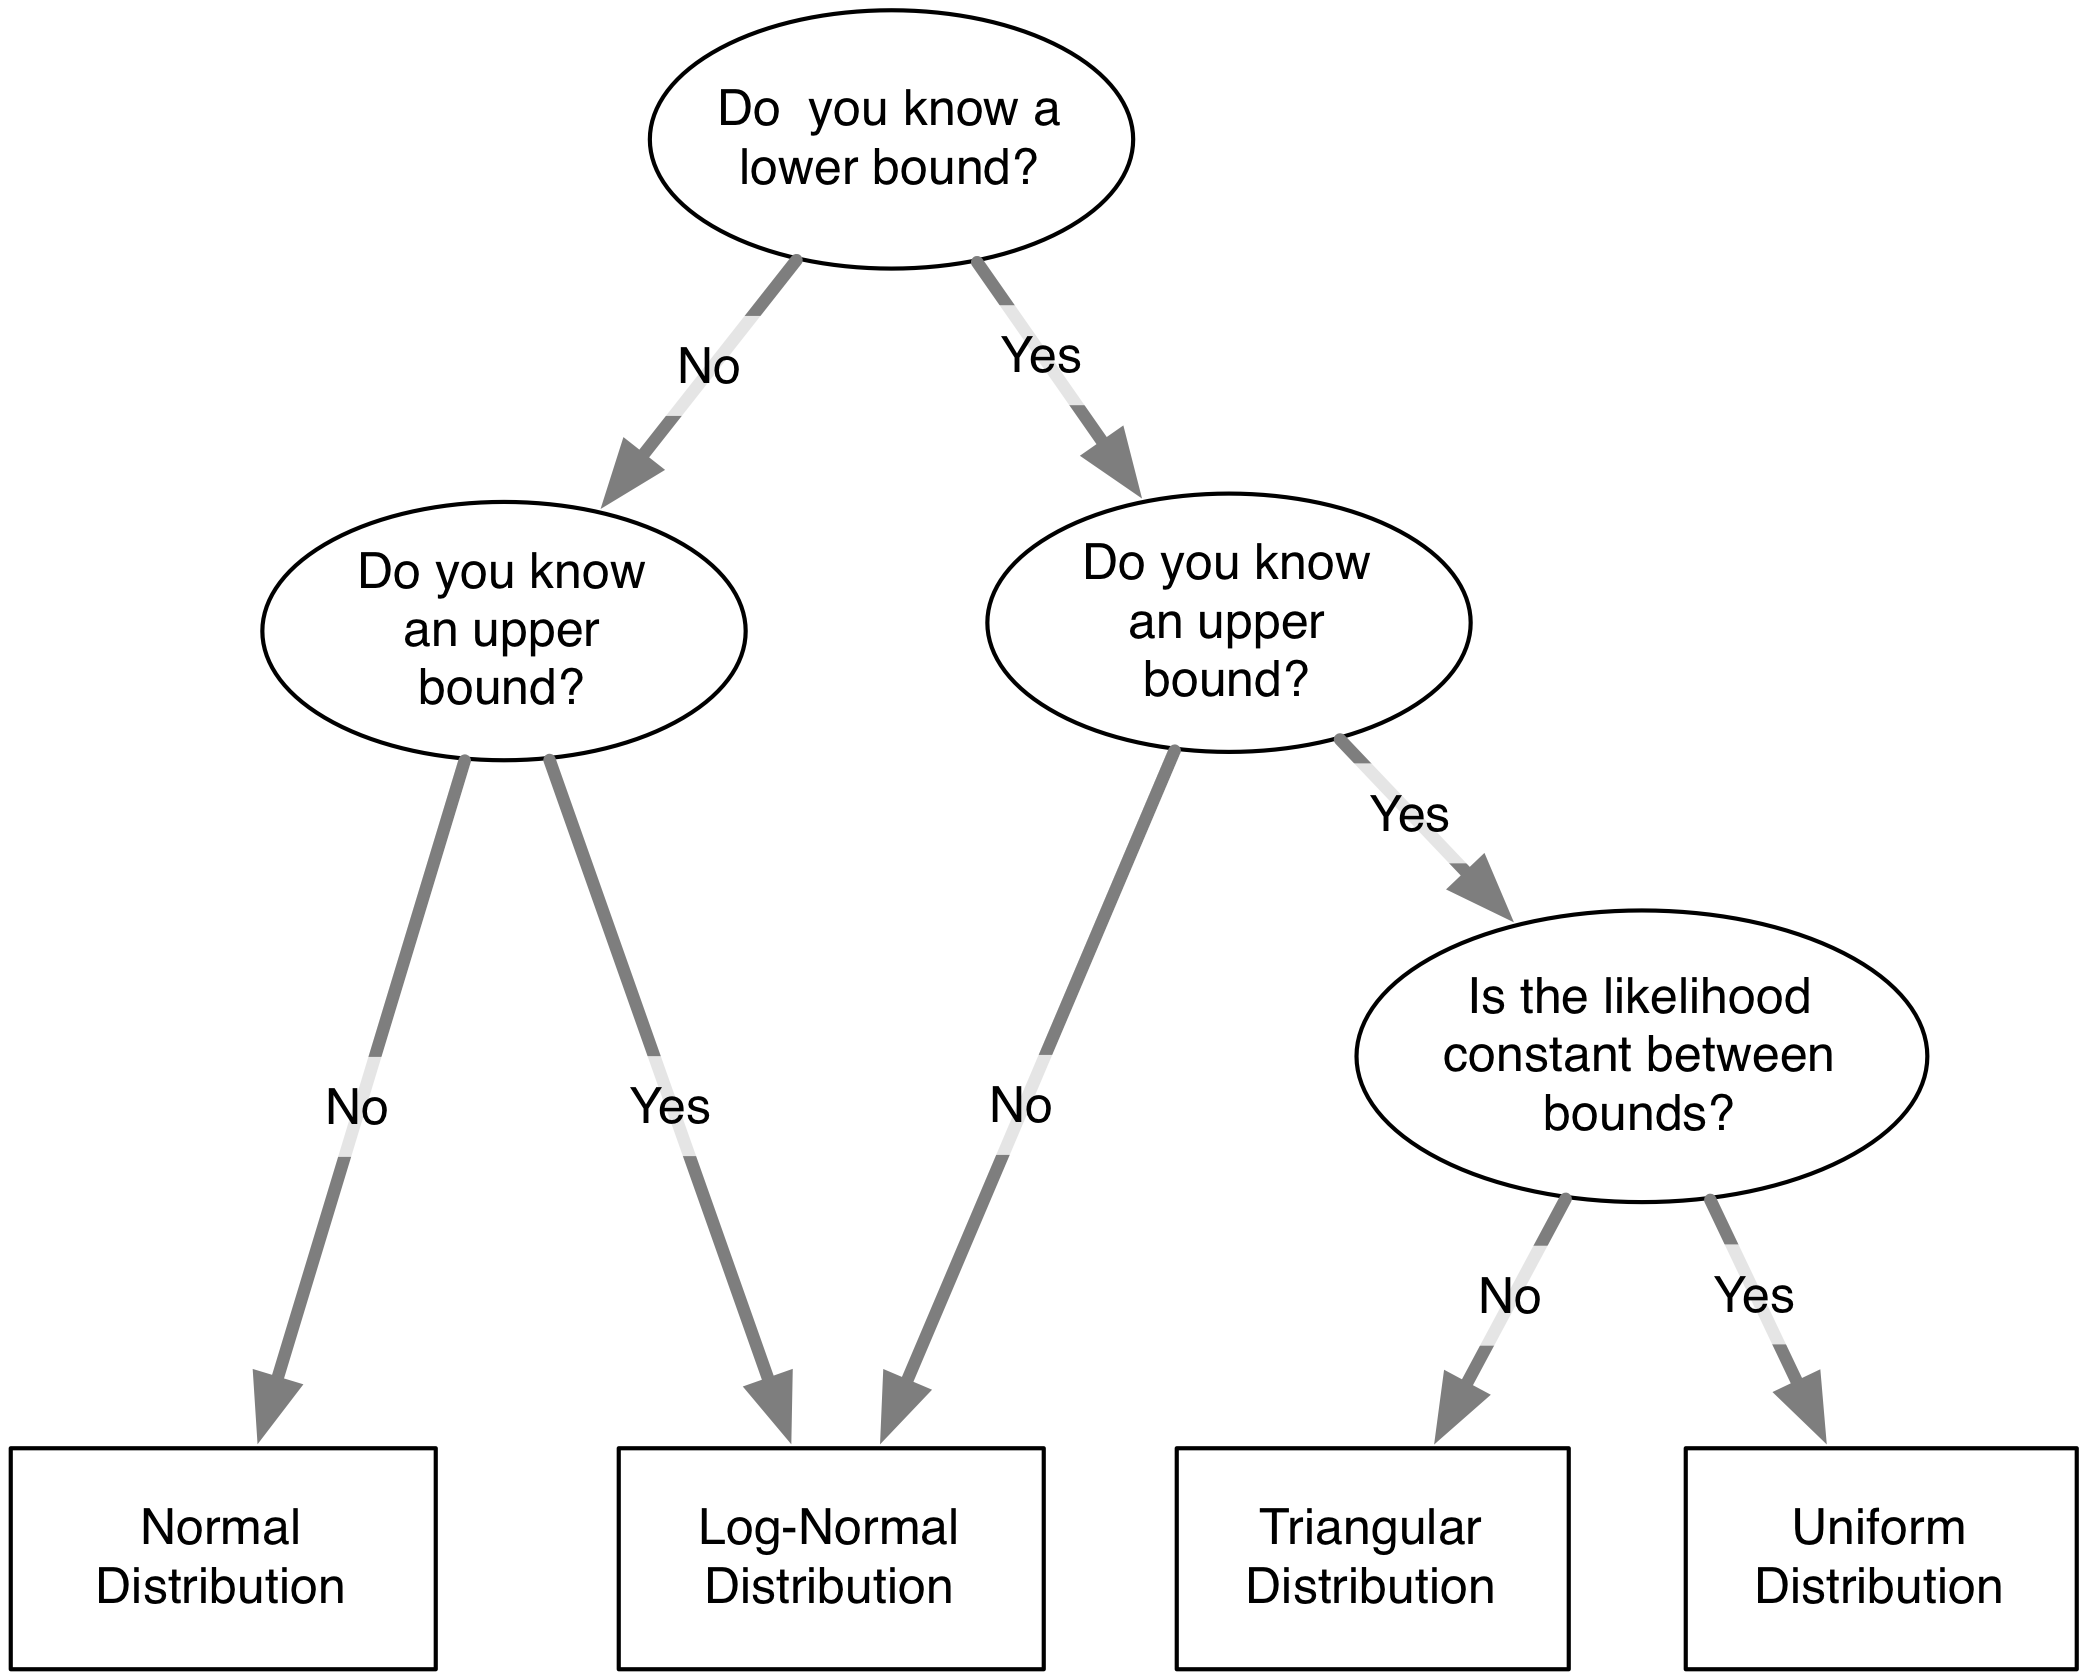
\includegraphics{DistributionsChoice.png}
\caption{Figure 2. Choices in Selecting a Distribution for a Variable's
Value}
\end{figure}

When important practical tip when using sensitivity testing within the
System Dynamics context is to be careful about specifying random numbers
within variables. The value of a variable is recalculated each time
step. This means that if you have a random number function in the
variable, a new random value will be chosen each time step. This can
create a problem if the random value is supposed to be fixed across the
course of the simulation. For instance, we may not know the birth rate
coefficient for our rabbit population, but, whatever it is, we assume it
is fixed over the simulation.

A simple way to handle these fixed variable values would be to replace
the variables with stocks. The stocks initial value could be set to the
random value and it would only be evaluated once at the beginning of the
simulation and kept fixed thereafter. This approach, though very
workable, however violates the fundamental metaphors at the hard of
System Dynamics. In Insight Maker, another approach is to use the
\lstinline!Fix()! function. When used with one argument, this function
evaluates whatever argument is passed to it a single time and then
returns the results of that initial calculation for subsequent time
steps. So instead of having the simple equation \lstinline!Rand(0, 10)!
in a variable to generate a random number between 0 and 10, you could
place \lstinline!Fix(Rand(0, 10))! in the variable. The first equation
would generate a new random number each time step, the second equation
will generate one random number and keep it constant throughout the
simulation.

\FloatBarrier 

\begin{model}[frametitle={Model: Sensitivity Testing}] 

 





Let's illustrate the usage of sensitivity testing using our rabbit example. First we will construct a simple exponential growth model.





\begin{enumerate}[label=\protect\circled{\arabic*}] \setcounter{enumi}{0}

\item Create a new \a{Stock} named \p{Rabbits}.


\item  Change the \a{Initial Value} property of the primitive \p{Rabbits} to \e{12}.


\item Create a new \a{Flow} going from empty space to the primitive \p{Rabbits}. Name that flow \p{Births}.


\item Create a new \a{Variable} named \p{Birth Rate}.


\item  Change the \a{Equation} property of the primitive \p{Birth Rate} to \e{0.05}.


\item Create a new \a{Link} going from the primitive \p{Birth Rate} to the primitive \p{Births}.


\item  Change the \a{Flow Rate} property of the primitive \p{Births} to \e{[Birth Rate]*[Rabbits]}.


\item The model diagram should now look something like this: \par \begin{minipage}{\linewidth}  \centering 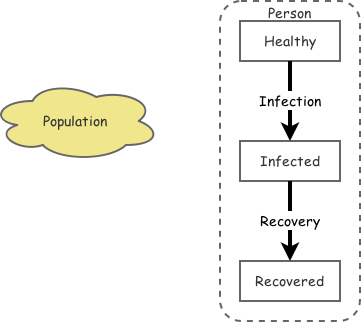
\includegraphics{model_34/diagram_11.png}
\end{minipage}




\end{enumerate} 



This is the basic outline for the model. We assume a fixed value of 12 rabbits and a fixed birth rate of 0.05.





\begin{enumerate}[label=\protect\circled{\arabic*}] \setcounter{enumi}{8}

\item Run the model. Here are sample results:\par \begin{minipage}{\linewidth}  \centering 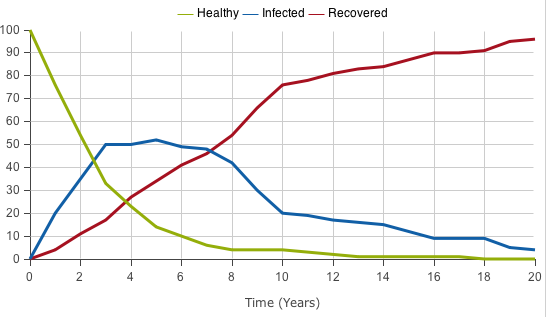
\includegraphics{model_34/result_13.png}
\end{minipage}




\end{enumerate} 



When we simulate we obtain the same results each time.





\begin{enumerate}[label=\protect\circled{\arabic*}] \setcounter{enumi}{9}

\item  Change the \a{Initial Value} property of the primitive \p{Rabbits} to \e{RandTriangular(6, 18, 12)}.


\end{enumerate} 



Now, let's try to incorporate uncertainty. Given that we know that there can be between 6 and 18 rabbits initially with an expected value of 12, we can use the \textbf{RandTriangular()} function to model this.





\begin{enumerate}[label=\protect\circled{\arabic*}] \setcounter{enumi}{10}

\item  Change the \a{value} property of the primitive \p{Birth Rate} to \e{RandLogNormal(0.05, 0.03)}.


\end{enumerate} 



We also do not know the birth rate with certainty. We know, however, that the rate must be greater than 0, and lets say we can assume the expected value is 0.05. We can use the \textbf{RandLogNormal()} function to model this type of uncertainty.





\begin{enumerate}[label=\protect\circled{\arabic*}] \setcounter{enumi}{11}

\item Run the model. Here are sample results:\par \begin{minipage}{\linewidth}  \centering 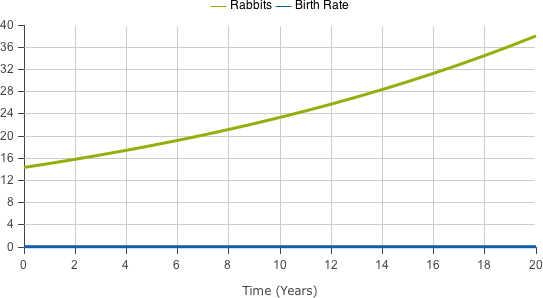
\includegraphics{model_34/result_19.png}
\end{minipage}




\item Run the model. Here are sample results:\par \begin{minipage}{\linewidth}  \centering 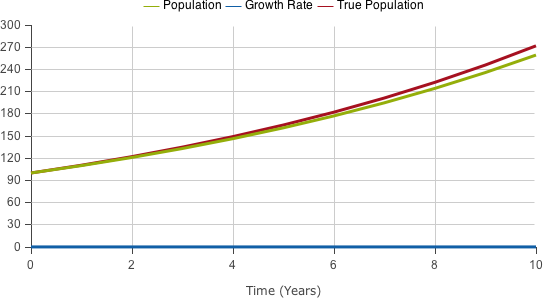
\includegraphics{model_34/result_20.png}
\end{minipage}




\item Run the model. Here are sample results:\par \begin{minipage}{\linewidth}  \centering 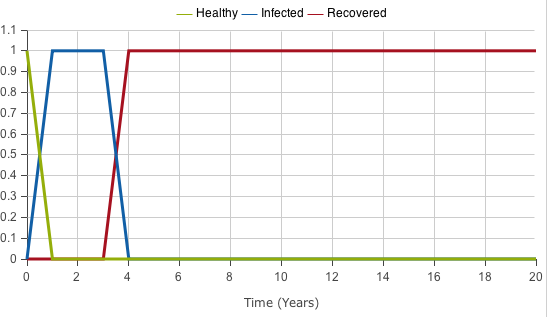
\includegraphics{model_34/result_21.png}
\end{minipage}




\end{enumerate} 



Now, we can simulate this mode a few times and see that each time we run the simulation we get a different result.







We can now use sensitivity testing to see the range of results given this specified uncertainty. We'll do 100 runs of the model and aggregate the results to see the expected distribution





\begin{enumerate}[label=\protect\circled{\arabic*}] \setcounter{enumi}{14}

\item \par \begin{minipage}{\linewidth}  \centering \includegraphics{model_34/data_25.png}
\end{minipage}




\end{enumerate} 



We can readily see the range of results allowing us to make decisions incorporating our known uncertainty about parameter values. 




 \end{model}

\hyperdef{}{Ex-9-2}{\paragraph{}\label{Ex-9-2}}

\beginEx{Exercise 9-2}

Create an equation to represent the uncertainty of how many red marbles
there are in a bag. You know there are at least 5 red marbles and no
more that 14. You do not have any other information.

\hfill{} \hyperref[Ans-9-2]{Answer Available}

\completeEx 

\hyperdef{}{Ex-9-3}{\paragraph{}\label{Ex-9-3}}

\beginEx{Exercise 9-3}

Create an equation to represent the uncertainty of how many red marbles
there are in a bag. You know there are probably about 20 red marbles and
you know there are no more than 100 marbles in the bag.

\hfill{} \hyperref[Ans-9-3]{Answer Available}

\completeEx 

\hyperdef{}{Ex-9-4}{\paragraph{}\label{Ex-9-4}}

\beginEx{Exercise 9-4}

Create an equation to represent the uncertainty of how many red marbles
there are in a bag. You know there are probably about 20 red marbles and
you do not know how many marbles the bag can hold total.

\hfill{} \hyperref[Ans-9-4]{Answer Available}

\completeEx 

The astute reader will notice that our discussion up to this has failed
to address an important point: how do we determine the uncertainty of a
variable? It is very easy to say that we do not know the precise value
of a variable, but it is much more difficult to define the uncertainty
of it. One case where we can precisely define uncertainty is when you
take a random sample of measurements. For instance, suppose our model
included the height of the average American man as a variable. We could
randomly select a hundred men and measure their heights. In this case
our uncertainty would be normally distributed with a mean equal to the
mean of our sample of one hundred men and a standard deviation equal to
the standard error of our sample of one hundred men\footnote{Please note
  that this contradicts slightly what we said earlier. Clearly, a person
  cannot have a negative height while the normal distribution will
  sometimes generate negative values. So wouldn't a log-normal
  distribution be better than a normal distribution? Mechanistically, it
  would, however statistically we can show that due to the Central Limit
  Theorem the normal distribution does asymptotically precisely model
  our uncertainty. Given a large enough sample size (100 is more than
  enough in this case), the standard deviations for uncertainty will be
  so small that the chances of seeing a negative number (or even one far
  from the mean) are effectively none.}. For any random sample of $n$
values from a population, the same should hold true: you will be able to
model your uncertainty using a normal distribution with:

\[ \mu = \frac{Value_1+Value_2+Value_3+...+Value_n}{n} \]
\[ \sigma = \sqrt{\frac{1}{n} \sum_{i=1}^n (Value_i-\mu)^2} \]

However, in most applied cases you will not be able to apply this
normality assumption. Generally you will not have a nice random sample,
or you might have no data at all and instead have some abstract variable
you need to specify a value for. In these cases, it is up to you to make
a judgment call on the uncertainty. Choose one of the four distributions
detailed above and use whatever expert knowledge available to you to
place an estimate on the parameterization of uncertainty. One rule of
thumb, however, is that it is better to overestimate uncertainty than
underestimate it. It is better to err on the side of overestimating your
lack of knowledge than it is to obtain undue confidence in model results
due to an underestimation of uncertainty.

\hyperdef{}{Ex-9-5}{\paragraph{}\label{Ex-9-5}}

\beginEx{Exercise 9-5}

You have tested the diameter of 15 widgets coming out of a factory and
obtained the following values: 2.3, 2.5, 1.9, 1.4, 2.0, 2.7, 1.9, 2.1,
2.1, 2.2, 1.6, 2.4, 2.0, 1.8, 2.6.

Create an equation to generate a new widget size with the same
distribution as the widgets arriving from the factory.

\hfill{} \hyperref[Ans-9-5]{Answer Available}

\completeEx 

\hyperdef{}{Ex-9-6}{\paragraph{}\label{Ex-9-6}}

\beginEx{Exercise 9-6}

You have taken 12 sheep from a population and weighed the amount of wool
on each sheep to obtain the following weights in kilograms: 1.005,
0.817, 0.756, 0.821, 0.9, 0.962, 0.692, 0.976, 0.721, 0.828, 0.718,
0.852.

Create an equation to generate how much a random variable for how much
wool you will obtain from a sheep.

\hfill{} \hyperref[Ans-9-6]{Answer Available}

\completeEx 

\section{Confidence and Philosophy}

The quality of a model in the eye of an evaluator is to a significant
extent influenced by the worldview (more or less coherent and the
philosophical orientation (if any) of the evaluator. Broad world-views
or epistemologies\footnote{From the Greek word ``epistēmē'' meaning
  ``knowledge'' or ``understanding'', epistemology is the branch of
  philosophy describing how we understand or come to know the world
  around us.} exist. One key divide in different epistemological
theories continues to be between those theories that contain a strong
belief in a concrete true reality that our knowledge can accurately
capture and those theories that believe our knowledge is partially or
wholly independent from reality.

Epistemological theories that are primarily in the first camp are those
such as positivism or empiricism. Theories in the latter camp include
constructivism and idealism. Constructivism is a popular theory of
knowledge that claims knowledge is constructed with social context and
historical time. Our presentation of confidence building for narrative
models in this chapter is implicitly in line with a constructivist
theory of knowledge.

In our discussion of confidence building we repeatedly refer to matching
the beliefs of the audience. We recommend creating simulations and
behavior in our models that match an audience's expectations for the
behavior of the system. This is distinct from saying that you should
match the reality of true system. Ideally, true behavior of the system
and an audience's mental models of the system should be equivalent, but
in practice they may well differ. Although confidence in a model will be
boosted by strictly matching the mental models of an audience, a truly
effective narrative model should be persuasive enough to change the
mental models of an audience.

Our discussion of predictive models from the previous chapter does not
fall within a constructivist world-view as we are claiming that there
are objective ``outside-ourselves'' measures of predictive accuracy we
can obtain. It should go without saying that predictive models may not
be accurate reflections of reality, even in their own terms. The
mathematics of a predictive model may be unrelated to the true system
that is being modeled, yet is may still create accurate predictions. As
such, our discussion of predictive models is not really a positivist or
empiricist one. Instead this discussion would fall under the
epistemological theories of pragmatism or instrumentalism which claim a
theory or model should be assessed on how well it predicts which may be
independent of the truth of the theory itself.

\paragraph{}

\beginEx{Exercise 9-7}

You are asked to evaluate a model simulating the growth of an endangered
species in its habitat. What tests and demonstrations would you like to
see in order to trust the model and recommend its use in practice?

\completeEx 

\paragraph{}

\beginEx{Exercise 9-8}

You are asked to evaluate a model simulating the potential adoption for
a new product at your company. The basic results of the model are very
encouraging for the product suggesting it would make a significant
return on investment.

What tests and demonstrations of the model would you like to see in
order to recommend the product be produced based on the model results?

\completeEx 

\hyperdef{}{ModelingProcess}{\chapter{The Process of
Modeling}\label{ModelingProcess}}

Now that you are well on your way to being a modeling expert, you may
begin to receive requests for assistance with various modeling projects.
As a motivating example, a friend -- it could also be a colleague or
client -- comes to you and asks for help. This friend has been involved
with the effort to protect the rare Aquatic Hamster.

The Aquatic Hamster is an endangered species that spends most of its
life living in lakes and rivers. Unfortunately, development and human
encroachment has steadily reduced the available habitat for these
hamsters and their population has plummeted. Indeed, now there is just
one last population of them left located on a lake just south of the
Canada/United States border.

Your friend asks you to build a model of this hamster population in
order to help prioritize protection efforts and to rally support from
governmental agencies and non-profits to protect this last hamster
colony. You want to be of real assistance to your friend, and the
hamsters are admittedly cute, so you agree to take on this modeling
project.

You are at your desk to start building the model, but then realize
something: You aren't sure what to do next. There are so many candidates
for first steps. Do you start sketching diagrams? Do you talk to hamster
experts? Do you start coding up a model? You are paralyzed by the sheer
number of different choices. You know your friend is counting on you, so
what do you do now?

In this chapter, we answer that question. We explore the modeling
process from start to finish, introducing the tools and techniques for
getting from ``I need a model'' to a final product that works. As you
will see, our experience is that the best approach to tackling tough
modeling problems is to start deceivingly small: build the simplest
model possible (what we call the ``Minimum Viable Model'') to get going
and then iterate aggressively on this initial version.

\section{Why Model?}

The first step to building a model is answering the simple question:
\emph{Why am I building this model?}

This question seems obvious, but it is often hard to answer in practice.
Let's try answering it for our hamster population model: Why are we
building this model? The truth is that so far we do not have a real
understanding of this.

Oftentimes, the lack of focus begins with the friend/client/colleague
who commissioned the model. Laypeople frequently do not have a strong
understanding of what modeling is,including what modeling can accomplish
and what it cannot. Instead, your friend might have a simplistic view of
a model, almost as if were a magic wand. He feels he just needs a model
and then, \emph{abracadabra}, it will solve his problem. His thought
process on what to do with a model might be as bareboned as:

\begin{enumerate}
\def\labelenumi{\arabic{enumi}.}
\itemsep1pt\parskip0pt\parsep0pt
\item
  Build Model.
\item
  \ldots{}
\item
  Hamsters Saved.
\end{enumerate}

Of course this is not the case. You build a model with a specific
purpose in mind otherwise it will most likely accomplish nothing. Worse
yet, when it comes to the hamsters, it will be too little too late. Your
first action should be to work with your friend to make sure you have
filled in the ``\ldots{}'' step. The best way to do this is generally
working backwards from the final step rather than working upwards from
the first one. For us that would be to first figure out how the hamster
population is to be protected.

Paradoxically, in order to answer the question of why we are building a
model, we are going to need to ask many questions of our own. Why should
we protect the hamsters? What risks do the hamsters face? What do the
hamsters need to be protected? What avenues to obtaining these
protections are there? What techniques to protecting the hamsters are
most effective? Cheapest? Most expedient? And so on. We need to obtain a
good understanding of the root cause of the problem you friend wants to
tackle with this model and force out the concrete steps to getting
there.

After discussing this with your friend and the two of you come to the
conclusion that you will need two things in order to reliably protect
the hamster population. First, government regulatory agencies need to
pass (stronger) rules protecting the hamster habitat. Second,
non-governmental organizations (NGO's) need to provide funds for hamster
conservation and protection efforts.

Using this, we can expand our plan with more details:

\begin{enumerate}
\def\labelenumi{\arabic{enumi}.}
\itemsep1pt\parskip0pt\parsep0pt
\item
  Build Model.
\item
  \ldots{}
\item
  Agencies enact rules to reliably protect hamsters. NGO's provide money
  for conservation efforts.
\item
  Hamsters Saved.
\end{enumerate}

This focuses things for us. Rather than ``Building a model to save the
hamsters'' (which is too vague and completely unactionable leading to
our quandary about what to model), we are building a model designed to
persuade governmental regulators and NGO's that they should devote
resources to protecting the hamsters.

So how do we do that? Let's simplify the complex issue into two specific
goals for our model:

\begin{itemize}
\itemsep1pt\parskip0pt\parsep0pt
\item
  Show that given the \emph{status quo} (business as usual) the hamster
  population will go extinct.
\item
  Show that alternatives to the \emph{status quo} exist (which require
  regulatory action or investments) that enable the hamster population
  not only to survive, but also to thrive.
\end{itemize}

If our model demonstrates both these things it could be a highly
persuasive tool to shape decisions and policies. By building a model
that does these two things\footnote{The model of course must also
  inspire confidence in its audience. They must believe its results are
  reliable otherwise the results will have no persuasive power. Review
  the previous chapter for tools for building confidence in models.} we
will have given our friend a powerful tool to push for regulatory action
and financial support.

When building your own models you'll want to go through a similar
thought process to get at the core goal or question the model should
address. Going into a modeling project with the attitude ``First we'll
build a great model, then we'll figure out how to apply it'' is a
prescription for failure. Of course, as you go through the process you
might discover insights you never expected or you might in fact
determine that your original hypothesis was wrong. Such discovery is
always a great outcome, but you can never count on it happening in the
course of building your model. It's best to start very focused in your
modeling efforts and treat any discoveries or broadening of scope later
on as a lucky bonus.

\section{Model Project Management}

When tackling modeling projects such as our hamster-population model,
there are two basic overarching project management approaches. The first
is founded on detailed planning and preparation. Tackling the hamster
model using this approach might look something like the following
sequential phases:

Research : Find and obtain relevant literature on Aquatic Hamsters. Read
peer-reviewed publications. Locate hamster experts and interview them.
Identify key mechanisms affecting hamster population growth. Some
mechanisms may require further study. For example, if human expansion
and urbanization affect the hamster habitat area, for example, you may
need to study the forces influencing urbanization. These may require
additional literature searches and expert interviews.

Design : Once you have completed your background research on the
hamsters, start to design the model. Create causal loop diagrams and
develop stock and flow diagrams. Break your hamster population model
into different sectors. You will have the hamster-specific sector, which
includes sub-sectors for each of the life-stages these endangered
hamsters go through. You will also need sectors for other parts of the
model that affect the hamster population growth: an urbanization sector
with its own model, a climate sector with a climate model, and so on.
Write out equations for all these sectors and resurvey experts you have
contacted to review the overall model design and the specific equations.
There will probably be several cycles of iteration and model expansion
during this stage as additional key areas to include are identified.

Construction : Now that you have completed a model design and received a
seal of approval from experts in the field, you are ready to start
building the model itself. Decide what modeling software package (or
programming environment) you will use. Implement the equations as they
were specified in the design phase.

Wrapping Things Up : Go through the confidence building steps from the
previous chapter. Develop tests for your model to ensure it works
correctly. Create model documentation. Show the model demonstrates
expected behavior and obtain final approval from experts.

This approach to building a model is a very linear process where you go
sequentially from stage to stage. In the project management field, this
is the classic ``waterfall'' project where you proceed phase by phase
through the project. You plan out the whole thing ahead of time
estimating how long each phase would take and identifying dependencies
between phases. This form of project management can work well if done
expertly and it is well suited for certain kinds of projects such as
constructing a building.

In our opinion, however, this approach to tackling a project is quite
poorly suited to the task of building a model. There are several reasons
for this.

First, each model is inherently unique\footnote{Lots of ``cookie
  cutter'' models out there are designed to model a certain class of
  problems. Without custom work, however, these models are of dubious
  validity and may serve more to ``check a box'' that a model has been
  built rather than to be a useful decision-making tool.}. You may have
developed a dozen different population models in your career, but when
it comes to developing a model for a new species or location, you will
inevitably run into situations and problems you have never encountered
before. The quantity and quality of data will differ from the cases
before. If not, the biology of the animal you are modeling will be
different. If not, the model goals and constraints will be different,
and so on. Given these differences, rigid project management techniques
such as the waterfall approach do not generally provide the
predictability that is needed.

Secondly, when building a model you will find that many of your
assumptions may simply be wrong. This can happen with every aspect of
model construction: the data you thought you had will turn out to be
non-existent, the equations provided to you by experts end up not
working, and the model code you write will invariably have a bug or two
that needs to be identified and squashed. Because of this you will
continually need to be adjusting and adapting your model as you learn
more about the system and what pieces of information you can rely upon
and what you cannot.

Such a high likelihood of error and need for readjustment are not well
suited towards techniques based on sequential, long-term planning
formats. What good is a great plan if the assumptions it is based on are
substantially wrong?

Take, for instance, the data you use to build your model. It is not
uncommon for a collaborator to come to you and say we have \emph{X},
\emph{Y} and \emph{Z} data series for you to use in your model (where
these might represent environmental conditions or other important model
inputs). When you go to check the data however you may find that in fact
\emph{X} does not exist (the collaborator was confused), \emph{Y}
actually has large gaps in the data set which make it effectively
useless for your needs, and \emph{Z} was collected in such a way that
they were actually measuring something completely different than they
thought they were.

Take, as another instance, the equations in a model. Imagine you consult
an expert on Aquatic Hamsters and she provides an equation governing the
survival of hamsters during their first year of life. This equation was
developed as part of a scientific study where the hamsters were grown in
indoor swimming pools at her university's Aquatic Hamster Research
Facility. When you go to apply this equation in your model, however, you
find out that how the hamsters behave when living within an indoor
swimming pool is very different from how they survive in the wild.
Because of this, the equation you have is simply not accurate for the
hamsters living in the wild.

Errors like these two examples are \emph{very} common. If you had
proceeded with the classic waterfall approach to modeling you might not
realize that you cannot rely on the data or equations you were planning
to use until the very end of the modeling process. At this point it is
much too late to go back and correct your model.

\subsection{Iteration: Failing Fast and Failing Often}

Because of this, we advocate an alternative approach to building models.
We support jumping right into the model construction process as early as
possible. As we showed you in the \emph{Red} example from Chapter 4, we
think it is important to get a simulation model up and running as
quickly as possible. You should never want to be more than a few steps
away from a simulating model\footnote{This is a common theme in agile
  approaches to project management. You never want to be far from a
  working product. For instance, in the popular Scrum approach to
  managing software projects, the key unit of collective work is ``the
  sprint''. A sprint is a relatively brief amount of time (in the scope
  of the entire project) to complete a set group of product features. At
  the end of the sprint, the features must be completed and the software
  working or they are cut. The goal is always to be close to a working
  program just like you should always be close to a working model.}.

When beginning a modeling project we recommend building the simplest
model possible to get going. We call this the \emph{Minimum Viable
Model}\footnote{This idea is adapted from Eric Ries's excellent book
  \emph{The Lean Startup} (Ries (2011)). In it he advocates an approach
  to developing start-up companies and businesses focus on rapid
  development and innovation. Ries supports developing a ``Minimal
  Viable Product'' for the company as quickly as possible and iterating
  on the feedback received for this initial product.} and it is the
model that contains just enough to minimally represent the system and
nothing more. For the hamster model, this Minimum Viable Model might
contain just a single stock representing the hamster population and a
couple of flows modifying the population. Nothing more.

You don't have to worry about your equations being right or your model
being an accurate predictor in the Minimum Viable Model; you just want
to get something up and running as soon as possible.

Once you have the Minimum Viable Model you can start to run it by people
and begin to incorporate their feedback. So get your friend's thoughts
on the minimal hamster model, talk to experts, study the model's
forecasts and see what works and does not. Then iterate on the model:
make a change here, add a new component there. If the feedback you are
getting is no one trusts the model because it does not contain some key
mechanism, add that mechanism to the model\footnote{But the key is to
  wait until you get this feedback. It's easy on your own or with a
  group of people to make a list of dozens mechanisms that a model
  \emph{must} contain to be realistic. Once you have implemented those
  mechanisms in your model you might find out that no one actually cared
  about them. It is best to start small and then augment the model when
  there is a demand for some additional mechanism, than it is to spend a
  large amount of time implementing a very complex model and then to
  find out much of that work was unnecessary.}. Steadily adjust and
refine the model based on the actual results of the model and the
feedback you receive.

This feedback will be more useful to you when you have a concrete model
that is simulating than it would be if you were just running abstract
ideas by people. By putting your stake in the ground with a model that
simulates, you allow others to critique and engage with the model
providing you with valuable information about what works and what does
not. If you do not come with a concrete model, you run the risk of
receiving very vague, unactionable feedback.

What is best about this approach of rapid iteration we advocate is that
it allows you to identify failures quickly. If a data source is no good,
you find that out immediately as you try to integrate it rather than
spending days, weeks or months planning your model with the assumption
it's really there or you can really use it. Rapid iteration -- failing
fast and failing often -- is a key goal in the model development
process. It can be argued that your successes in life are directly
proportional to the number of failures and wrong turns you take: the
more things you try, the more times you will both succeed and fail. We
believe the same is often true in modeling. By speeding up the process
of identifying and iterating past failures, this agile approach to
modeling will often result in higher quality models completed more
quickly than approaches that rely on extensive planning.

\section{Model Boundaries}

There are many different mechanisms and entities we could include in our
model of the hamster population\footnote{The idea of the ``butterfly
  effect'' is that the flapping of a butterfly's wings in Europe, can
  initiate slight air disturbances that interact and magnify until they
  create a hurricane in Florida. If we believe in such avalanche effects
  to small events, the number of potential items we should include in
  the model is literally endless.}. Of course there are the hamsters
themselves but there are also hamsters predators, the hamsters' food,
climatic conditions that affect the growth and survival of the hamsters,
urbanization, eutrophication that affects the hamsters' lake, and so on.
Given that it would be impossible to include every single element and
mechanism in our model, we must define the boundaries of the system.

\begin{figure}[htbp]
\centering
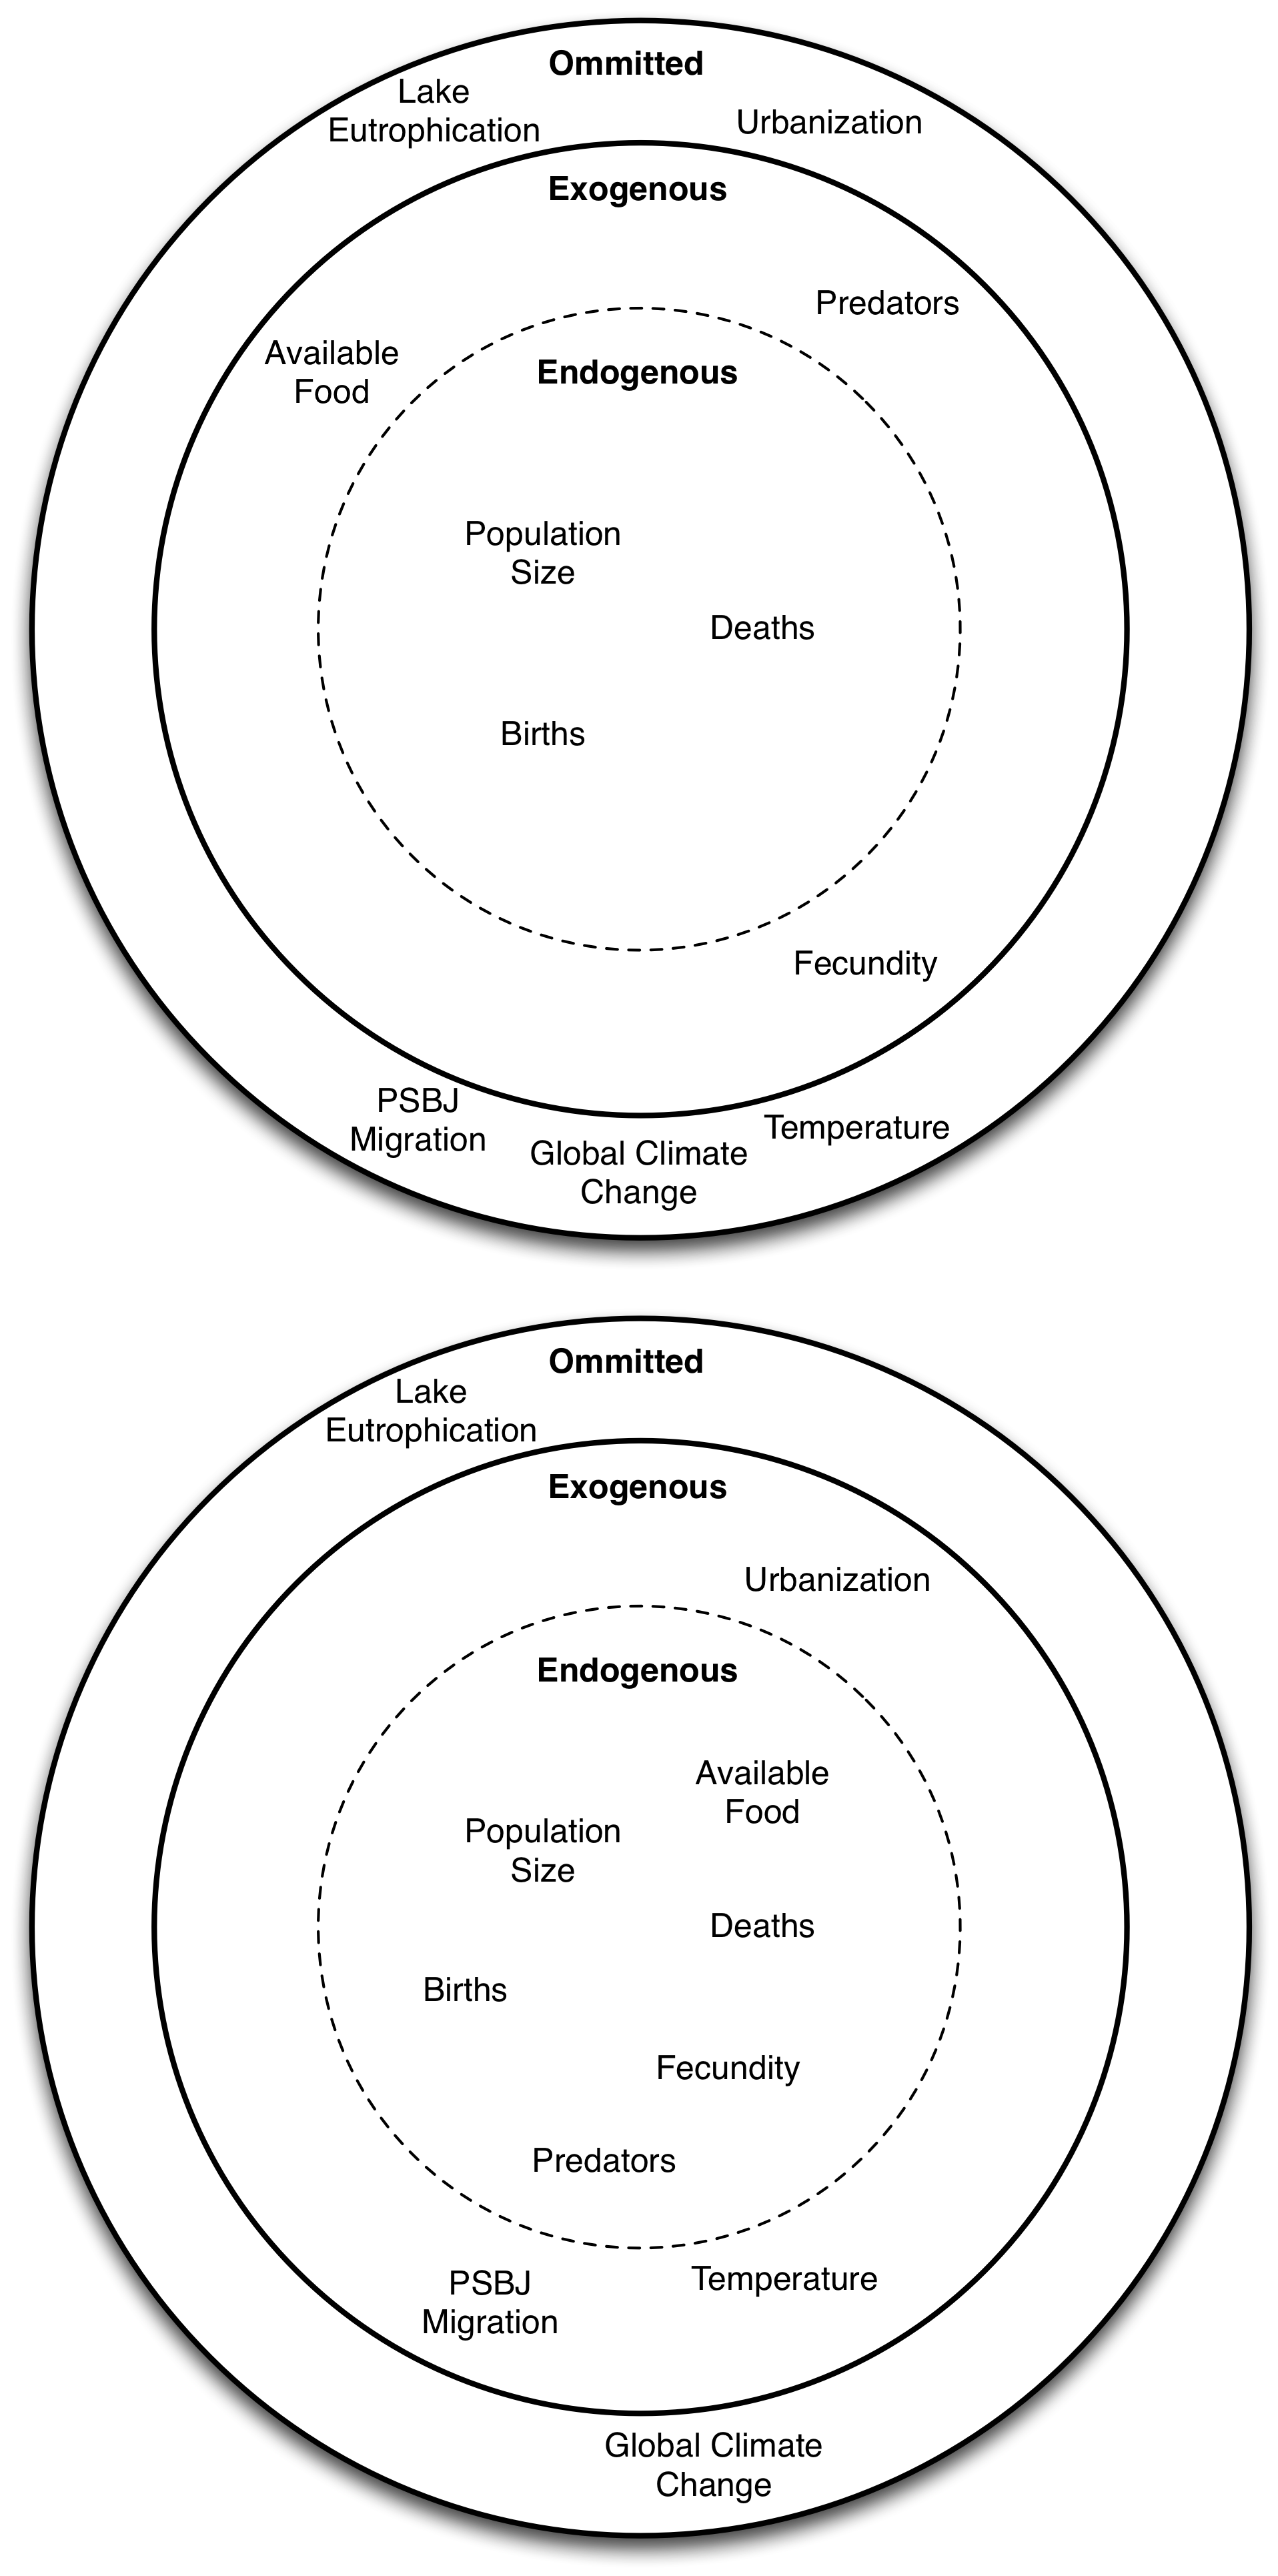
\includegraphics{Boundaries.png}
\caption{Figure 1. Two different sets of boundaries for the hamster
population model.}
\end{figure}

We can illustrate model system boundaries using a boundary diagram as
illustrated in the excellent book \emph{The Electronic Oracle} (Meadows
and Robinson (1985))\footnote{This book provides an excellent overview
  of a number of different models and, very interestingly, it tracks the
  ultimate reception and the success or failure of these models.}. When
using a model boundary diagram, we classify items of interest into one
of three categories:

Endogenous : Endogenous items are at the core of the model. They are
things that the model itself determines. For instance, the size of the
hamster population is endogenous to the model. The model itself
simulates this population.

Exogenous : Exogenous items are those that you include in the model but
which you do not directly simulate. For instance, if we thought
temperature had a significant effect on hamster survival, we might want
to include historical temperature data in the model. We do not want to
simulate this data though, we just want to use it as an exogenous input
into the model.

Omitted : Omitted items are those that, though we may acknowledge they
do impact the hamsters either directly or indirectly, we choose not to
include in the model. Even the most ambitious and comprehensive model
will need to draw the line somewhere.

Figure 1 illustrates two different model boundaries for the hamster
model. The top diagram depicts a small, conservative model with many
features excluded from the model. The bottom figure illustrates a much
more ambitious model where many additional items are made endogenous to
the model and there are much fewer omitted items.

When developing a model, we recommend starting with the boundaries as
narrow as possible. In the minimum viable model, you will want to omit
as many different mechanisms as possible. As you receive feedback and
people push for the inclusion of different mechanisms, you can slowly
expand the boundaries of the model. We recommend starting small and
expanding as necessary.

\paragraph{}

\beginEx{Exercise 10-1}

Create a boundary diagram for a model of human population growth in the
next 100 years. What would be the endogenous, exogenous and omitted
items in this model.

\completeEx 

\paragraph{}

\beginEx{Exercise 10-2}

Create a boundary diagram for a model forecasting the total quantity of
pencils sold within the united states for the next 50 years. What would
be the endogenous, exogenous and omitted items in this model.

\completeEx 

\section{From Mental Models to Simulation Models}

Generally speaking, a single individual should ultimately be responsible
for the design and implementation of a model. Models
``designed-by-committee'' are understandably suffused with compromise
and a greater lack of focus. That said, even though one person is
ultimately calling the shots, many voices and perspectives are there to
be heard in the modeling process. The more input there is into a model,
the better the resulting model will most likely be.

The people you are working with generally will not be experts in
modeling. Because of this, even if they are intimately familiar with the
system you are attempting to model, it will sometimes be difficult to
take their freeform insights and transform them into a formal model
structure and accompanying numerical equations. In fact people often
have great difficulty communicating and describing their own mental
models of a system. A number of useful tools and techniques can be used
to help elicit information on people's mental models. We discuss three
of these tools in the following sections.

\subsection{Reference Mode Diagrams}

A reference mode is a graph that plots how the key stocks and variables
in the system change over time. The \emph{x}-axis of the graph is time,
and the \emph{y}-axis shows the values of the variables as they change.
Sometimes reference modes are based on historical data, but you can also
create them by asking those involved with the system to sketch out how
they think the system will behave in different scenarios.

For our hamster model we could start simply by asking our friend to
sketch out what he thinks will happen with the hamster population in the
future assuming business as usual (remember that the status quo does not
mean no-action). When we do this, he sketches out the top graph in
Figure 2.

While your friend probably would use different terminology, to us the
curve he sketched immediately looks like an exponential decay model. The
instant we see this sketch we should start mapping out a stock and flow
diagram in our mind to implement this type of model. Your friend does
not need to understand any modeling concepts though, he just needs to be
able to draw a picture of what he thinks will happen in the future. This
is something that is easy to ask most people to do.

\begin{figure}[htbp]
\centering
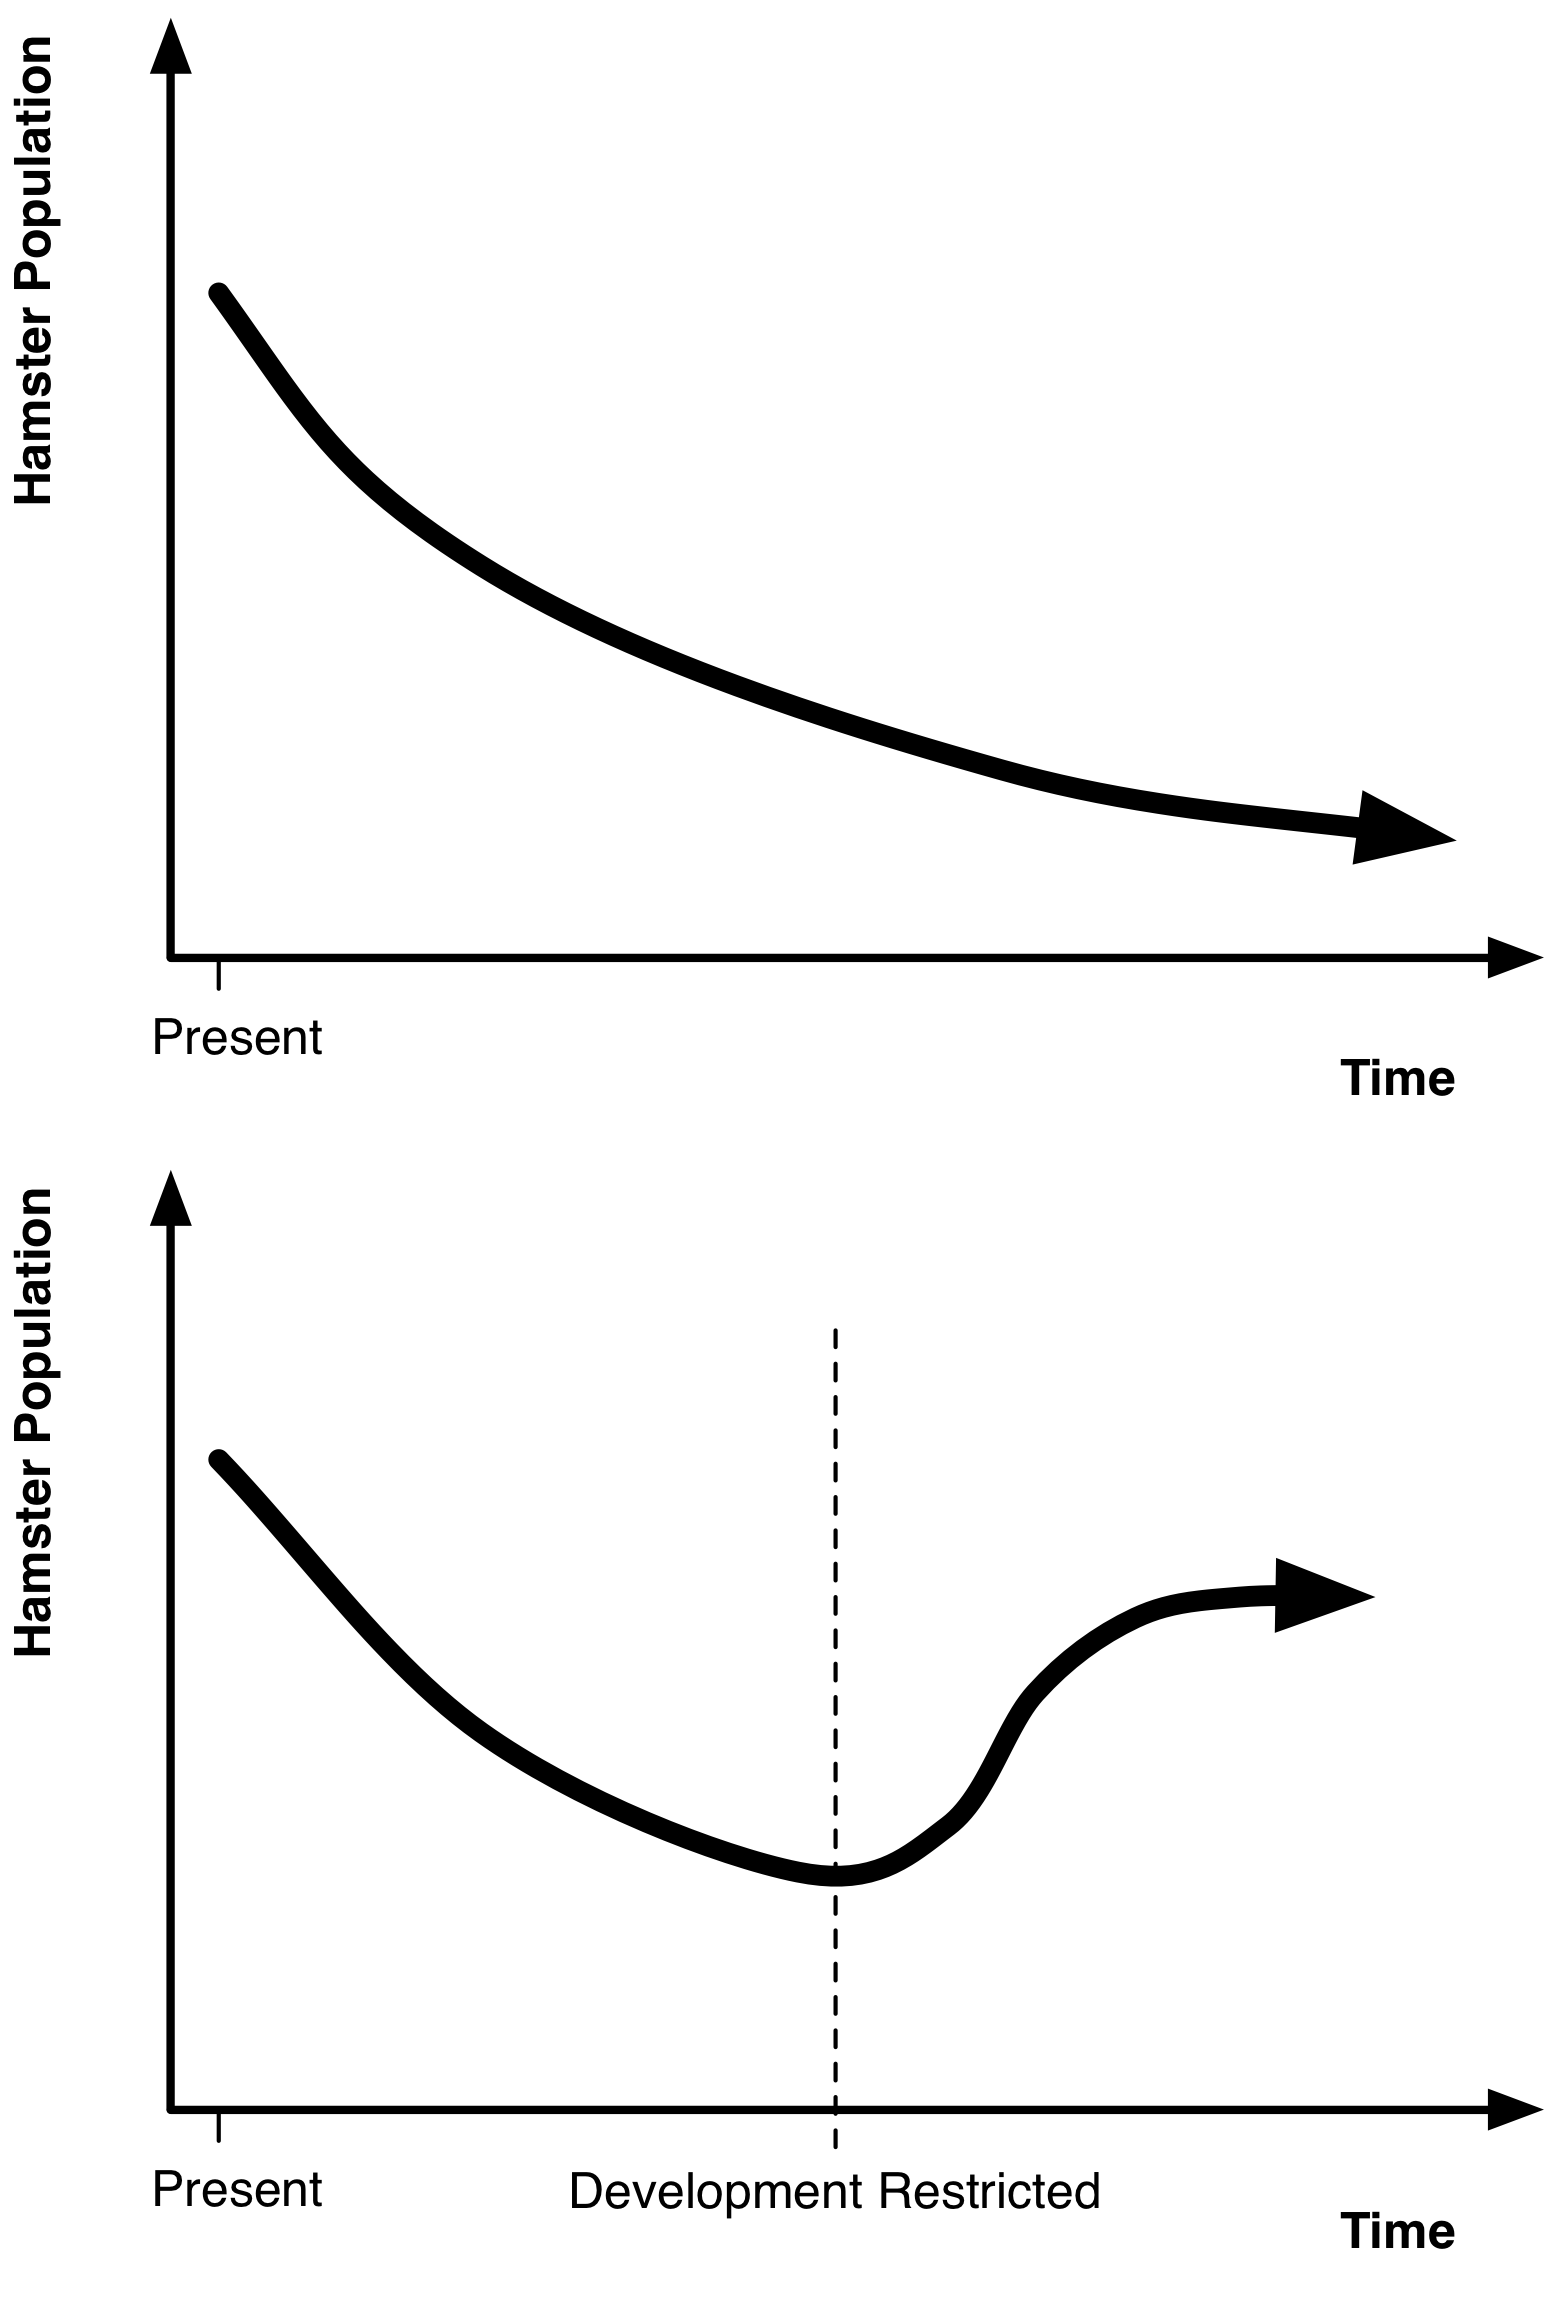
\includegraphics{ReferenceModes.png}
\caption{Figure 2. Sample reference modes for our hamster model.}
\end{figure}

Let's go beyond the simple business as usual scenario. We can also use
reference mode diagrams to elicit information on different scenarios.
For instance, we have previously been told that development and
encroachment on the hamster habitat are key factors reducing the hamster
population size. Not only does the development consume key hamster
habitat, the construction creates disturbances that have a further
negative impact on the hamsters.

We can ask our friend to create a second sketch that shows how the
hamster population would respond if development were suspended
indefinitely. He responds by drawing the bottom graph in Figure 2. This
graph shows the hamster population starting to recover after development
stops, initially growing and then leveling off at a certain point.

Again, your friend never said this, but looking at this second drawing
we should immediately start thinking of logistic growth models. The
leveling off implies that there is some carrying capacity limit for the
hamsters. This carrying capacity is probably a function of the available
hamster habitat and the disturbances that are going on around the
hamsters. We can start to sketch out stock and flow and causal loop
diagrams to implement these types of dynamics and reproduce the
behaviors our friend has drawn.

These are just two of the reference modes we might ask our friend to
think about. We could go on to explore other scenarios and see how he
thinks the changes in the scenarios would affect the hamster population.
We could also ask him to sketch out other key variables in the system --
such as the quantity of food available to the hamsters -- to understand
how he thinks these key variables interact. We could go on to interview
other people familiar with the system and take them through the same
process. Ideally, all the reference modes between individual people will
agree, but differences are in themselves also useful in revealing
different mental models between our interviewees. Bridging differences
will be a key interest of ours as we attempt to develop a persuasive
model that will bring everyone on board and gain wide support.

Asking non-modelers to sketch out reference modes is a great technique
for several reasons. Reference modes are accessible to laypeople, force
your interviewees to be concrete, and provide you with very useful and
actionable material. Really, a reference mode is a projection of an
individual's mental model of the system. They may be unable (or
unwilling) to explain their mental model to you in equations or even
words, but they generally will be able to describe how they perceive the
world using these reference mode diagrams -- one small slice of their
mental model at a time. Once you have the diagrams, you can proceed to
translate them into model structure and equations.

\paragraph{}

\beginEx{Exercise 10-3}

Draw a reference mode diagram for what you will think will happen to the
total human population in the next 100 years. Draw additional reference
modes for the following scenarios:

\begin{enumerate}
\def\labelenumi{\arabic{enumi}.}
\itemsep1pt\parskip0pt\parsep0pt
\item
  Cold fusion is invented in 2050. Limitless energy is available for
  free to everyone.
\item
  A plague wipes out 1/2 the human population in 2035. Each country is
  affected equally by the plague.
\item
  A process for cheaply converting a drop of oil directly into a
  kilogram of nutritious and delicious food stuffs is invented in 2030.
  This can replace the need for arable land, but oil become in even
  greater demand.
\end{enumerate}

\completeEx 

\paragraph{}

\beginEx{Exercise 10-4}

You are hired by a paper company to create a model of paper consumption
in the next fifty years. Draw reference mode diagrams of world paper
demand for the most highly likely future scenarios as you see them.
Consider the adoption of digital technologies and the decline of print
media.

\completeEx 

\subsection{Pattern-Oriented Modeling}

Pattern-oriented modeling focuses on identifying key patterns in the
system to be modeled. For example, we may observe a boom-and-bust
pattern in our hamster population that is triggered by unusually warm
weather. When we develop our model, we formulate relationships and
equations that will replicate this boom-and-bust pattern in the
simulation.

Developed to help guide the creation of agent-based models,
pattern-oriented modeling is very similar in concept to reference modes
and system archetypes. Rather than building models around expected
dynamic trajectories however, pattern-oriented modeling builds models to
recreate patterns. Sometimes a pattern may be the same as a reference
mode, but especially when dealing with agent based modeling you may not
be able to define a pattern in terms of the dynamic trajectory of a
reference mode. For a good overview of pattern-oriented modeling, see
Grimm (2005).

\paragraph{}

\beginEx{Exercise 10-5}

What patterns might you see in the how cities are located?

\completeEx 

\paragraph{}

\beginEx{Exercise 10-6}

What patterns might you see in the movement of a carnivore like a wolf?
In an herbivore like a moose?

\completeEx 

\paragraph{}

\beginEx{Exercise 10-7}

What patterns might you see in the movement of a competition between
companies in an expanding market? In a contracting market?

\completeEx 

\subsection{Group Model Building}

Group modeling sessions are a powerful tool to capitalize on the
collective thoughts of a group to inform model structure and design.
Instead of individually surveying experts and those involved in a
system, a group session with many interested parties can be conducted.
The term ``group model building'' is a bit of a misnomer as generally
the model itself will be built away from the group by the facilitator or
modeler and the group work will be focused on identifying and ranking
key variables and mechanisms and developing high-level causal loop or
stock and flow diagrams. See Andersena and Richardsona (1997) for a very
practical overview of running and facilitating group model building
sessions.

Group modeling sessions can also benefit an organization independently
of the success or failure of the model itself. You might expect that the
mental models of individuals within an organization would be aligned and
the members of the organization would share a common objective and
understanding of the challenges and needs required to achieve this
objective. However, this is often not the case as different organization
members may hold distinct mental models of the organization's purpose
and operation within the world. Additionally, it is quite possible that
these differences may never be realized as people may fail to adequately
communicate their mental models assumptions and beliefs during the
course of regular interactions.

The group modeling process can force the concrete discussion of and
revealing of these mental models and the stakes involved in having these
differences. Once they are revealed, they can be discussed and
reconciled, potentially leading to a greater congruity of viewpoints
within the group and a greater shared purpose. Vennix, Scheper, and
Willems (1993) carried out a survey of participants in group model
building sessions and found that this process led to insights and a
shared vision more quickly than occurred in standard meetings.

\section{Wrapping it Up}

Completing a model is in some ways just the first step in a modeler's
work. Once the model is finished you need to make sure to develop
adequate tests to ensure it is operating as designed. Moreover, a model
by itself is often of little use. You will need to develop extensive
sets of documentation, manuals and tutorials if you want the model to be
used in practice by people other than yourself. Such efforts take time.
Writing clear and useful documentation is a skill in itself and, if done
right, may take as long as developing the model in the first place!

In general, it is important to remember the 80/20 rule which also
applies to modeling. The first 80\% of modeling work generally only
takes 20\% of the time while the last 20\% of the work can take four
times as long. Getting the small details right in a model can take much
longer than implementing the bulk of the model structure.

\paragraph{}

\beginEx{Exercise 10-8}

You have been asked to model crime trends in a major city. Write out a
general overview of stages you might take to developing this model from
start to finish.

\completeEx 

\chapter{The Mathematics of Modeling}

This chapter takes the modeling techniques introduced earlier in this
book and places them within a firm mathematical framework. The contents
of this chapter are quite technical in parts and to fully understand
them requires knowledge of basic calculus and linear algebra. We present
the material because it is important for both readers who want a deep
understanding how their models operate and also those who wish to
understand how System Dynamics fits within the larger field of
mathematical modeling. For users who approach systems thinking and
modeling from a more qualitative angle, this material may be browsed or
safely skipped.

\section{Differential Equations and System Dynamics}

Differential equations are a common mathematical tool used to study
rates of change. Some basic terminology needs to be learned in order to
discuss differential equations. After introducing this new terminology,
we will then tie it back to the modeling techniques you've already
learned.

State Variable : A state variable is an object that represents part of
the state of a system. For instance, in a population model you could
have a state variable representing the current number of individuals in
that population. In a model of a lake, you could have a state variable
representing the current volume of water in the lake. In equations,
state variables are often represented using Roman letters such as $X$,
$Y$ or $Z$.

Derivative : Derivatives define rates of change in state variables. For
instance, if we had a state variable representing the size of a
population, a derivative would specify how this population grows or
shrinks over time. The population's derivative would aggregate all
changes such as births, deaths and immigration or emigration to show the
net change in the state variable over time. Similarly, in the case of a
model of a lake, the lake volume state variable would have a derivative
showing how much net water flows into or out of the lake over time.
Given a state variable $X$, the derivative of $X$ with respect to time
is generally written as $dX/dt$ but can also be written as $X'$ or
$\dot{X}$.

Let's put this new terminology to work to define a simple model. We
start by creating an exponential growth population model. We only need
one state variable in this model to represent the size of the
population. We denote this state variable as $P$. We need to define one
parameter to control the growth rate in the population. We will denote
this growth rate parameter $\alpha$.

The resulting differential equation exponential growth model can be
written simply as:

\[ \frac{dP}{dt} = \alpha \times P \]

This indicates that the rate of change for the population for one unit
of time is $\alpha \times P$. Our model is not quite fully specified yet
as we do not know what the initial value of the population is.
Differential equation models are often additionally specified by
providing the values of the state variables at a specific point in time.
Below we indicate that the population size at time 0 is 100.

\[ P(0) = 100 \] \[ \frac{dP}{dt} = \alpha \times P \]

You may have already noted that this model is easy to construct using
the techniques we have already introduced in the book. In fact we have
discussed this type of model several times. We could construct it with
System Dynamics tools using a stock to represent the population ($P$), a
flow to represent the change of population ($dP/dt$) and a variable to
represent birth rate ($\alpha$). We could specify our initial condition
of a population size of 100, by setting the initial value for the stock
for 100.

This is an important point. Many differential equation models\footnote{Specifically
  those where the denominator in the derivative $dX/dt$ is always $dt$:
  a very wide class of commonly used models.} can be directly
represented using the System Dynamics modeling techniques described in
this book. Similarly, a System Dynamics model can be rewritten as a
differential equation model.

From this perspective, System Dynamics models and differential equation
modeling are one and the same. A System Dynamics model can be expressed
using differential equation notation and vice versa. To see this in more
detail, we can look at the mapping between System Dynamics and
differential equation models. There is a one a one-to-one direct
correspondence between the key System Dynamics primitives and components
of a differential equation model.

\begin{longtable}[c]{@{}ll@{}}
\hline\noalign{\medskip}
System Dynamics Primitive & Differential Equation Equivalent
\\\noalign{\medskip}
\hline\noalign{\medskip}
Stock & State Variable ($X$, $Y$, etc\ldots{})
\\\noalign{\medskip}
Flow & Derivative ($dX/dt$, $dY/dt$, etc\ldots{})
\\\noalign{\medskip}
Variable & Constants/Parameters ($\alpha$, $\beta$, etc\ldots{})
\\\noalign{\medskip}
\hline
\end{longtable}

Since they do not differ significantly from a mathematical standpoint,
what separates these two approaches to modeling? Where System Dynamics
and differential equation modeling differ is in their focus and
philosophy. The primary goal for differential equation modelers is
analytic tractability (in other words, how easy is it to mathematically
manipulate and understand the model's equations). This analytic
tractability allows these modelers to derive definite results and
conclusions from the model's equations. System Dynamics modelers
generally are less concerned about analytic tractability and are more
comfortable with simulating the model and drawing conclusions from
observed trajectories and numerical results.

System Dynamics modelers, to go further, care greatly about
communicating their models, deliberately mirroring reality to some
extent and exploring the consequences of feedback. The differing focuses
on communication between System Dynamics modelers and differential
equation modelers can be seen in the method of naming variables.
Differential equation models are generally dominated by abstract Greek
symbols (e.g. $\alpha$) while System Dynamics models generally clearly
spell out variable names (e.g. ``Birth Rate'') and additionally use a
model diagram to illustrate and communicate the relationships between
different parts of the model.

\hyperdef{}{Ex-11-1}{\paragraph{}\label{Ex-11-1}}

\beginEx{Exercise 11-1}

You have a System Dynamics model simulating water leaking out of a hole
in a jar. You have a stock \p{Jar} with an initial value of 40. Roughly
10\% of the water leaks out of the jar every time period and there is a
single flow leading out of the jar with the rate \lstinline!0.10*[Jar]!.
Express this model using differential equations.

\hfill{} \hyperref[Ans-11-1]{Answer Available}

\completeEx 

\hyperdef{}{Ex-11-2}{\paragraph{}\label{Ex-11-2}}

\beginEx{Exercise 11-2}

You have a System Dynamics model simulating people becoming sick. You
have two stocks in the model \p{Healthy} and \p{Infected}. There is a
single flow, \p{Infection}, going from the healthy to infected stock
with a flow rate of \lstinline!0.05*[Infected]*[Healthy]!. Initially
there are 100 infected people, and 1 infected person. Express this model
using differential equations.

\hfill{} \hyperref[Ans-11-2]{Answer Available}

\completeEx 

\hyperdef{}{Ex-11-3}{\paragraph{}\label{Ex-11-3}}

\beginEx{Exercise 11-3}

You have a differential equation model of an animal population's growth
(denoted $P$). The animals growth is parameterized by the parameter $r$
and a maximum population size or carrying capacity of $K$. The following
differential equations define this model:

\[P(0) = 500\] \[r = 0.05\] \[K = 10000\]
\[\frac{dP}{dt}=r P \left(1-\frac{P}{K}\right)\]

Implement a System Dynamics version of this model. What is the size of
the population after 100 years?

\hfill{} \hyperref[Ans-11-3]{Answer Available}

\completeEx 

\section{Solving Differential Equations}

Given a differential equation or System Dynamics model specification,
how do you go about determining the results of the model? This is
typically referred to as ``solving'' the model. Since differential
equation models and system dynamics models are essentially one and the
same, the techniques used to solve differential equations can be
directly applied to System Dynamics models and they are the techniques
used by Insight Maker when you simulate any of the models in this book.

For most of the rest of this chapter, we use the differential equation
terminology instead of the System Dynamics one. We do so first because
it is more concise and more elegantly addresses the issues discussed in
this chapter, but also because we want to familiarize you with its
terminology and concepts. If you ever get lost, just refer to the System
Dynamics to differential equation translation table we showed above.

Let's start our discussion of solving differential equations using our
simple population model. As you recall, this model was:

\[ P(0) = 100 \] \[ \frac{dP}{dt} = \alpha \times P \]

What is the size of the population, at, let's say $t=10$ given an
$\alpha$ of 0.1? Calculus can be used to solve the model and answer this
question. First we separate the terms of the derivative and integrate
both sides of the equation. Thereafter it is a simple matter of algebra
to solve for $P$:

\[
\begin{aligned}
\frac{dP}{dt} &= \alpha \times P \\
dP &= \alpha \times P\ dt \\
\frac{1}{P}\ dP &= \alpha\ dt \\
\log(P) &= \alpha \times t + A \\
P &=  e^{\alpha \times t + A} \\
P &=  B \times e^{\alpha \times t} \\
\end{aligned}
\]

In this equation two new variables $A$ and $B$ appeared (where we
arbitrarily set $B=e^A$). These are unknown integration
constants\footnote{Recall from calculus that if $A$ is a constant, then
  $x^2+A\ dx = 2 \times x$. When we integrate $2 \times x$ we need to
  add back in the constant term. We don't know the value of this
  constant term immediately and we have to determine it later on.}. We
can determine the values of the integration constants based on the
initial conditions of the model, as we specified earlier that
$P(0) = 100$. We evaluate the solution of the model at this initial
condition to determine the value of $B$.

\[
\begin{aligned}
P &= B \times e^{\alpha \times t} \\
100 &= B \times e^{\alpha \times 0} \\
100 &= B
\end{aligned}
\]

Thus our generic equation for $P$ at any time and for any $\alpha$ is:

\[ P = 100 \times e^{\alpha \times t} \]

Plugging in $\alpha=0.1$ and $t=10$, we obtain:

\[
\begin{aligned}
P &= 100 \times e^{0.1 \times 10} \\
  &= 271.828...
\end{aligned}
\]

For this simple population model we have shown that we can obtain the
precise population value at any point in the future. It took a fair
amount of algebra even for such a simple model, but we did it!

Unfortunately, many differential equation models cannot be solved using
these techniques. For most complex models in practice, it is impossible
to analytically determine the values of the state variables in the
future. This inability to solve a model can be true for even very simple
models. Take for example the following growth model similar to our
original one:

\[ P(0) = 100 \] \[ \frac{dP}{dt} = \alpha \times P \times \log(P) \]

We have simply added a logarithm of $P$ into our growth rate. Despite
the smallness of this change, this model is now impossible to solve
analytically. There is no analytic solution possible, but feel free to
give it a try yourself (but please don't try too hard; we promise there
is no solution). When developing complex models it should generally to
be assumed that in practice no analytical solution will be available. In
cases like these, how can we go about developing solutions to the
equations and determining the trajectory of the state variables in the
system?

\hyperdef{}{Ex-11-4}{\paragraph{}\label{Ex-11-4}}

\beginEx{Exercise 11-4}

Solve the differential equation:

\[ P(0) = 10 \] \[ \frac{dP}{dt} = -\alpha \]

\hfill{} \hyperref[Ans-11-4]{Answer Available}

\completeEx 

\hyperdef{}{Ex-11-5}{\paragraph{}\label{Ex-11-5}}

\beginEx{Exercise 11-5}

Solve the differential equation:

\[ P(0) = 10 \] \[ \frac{dP}{dt} = 0.05 \times P \]

\hfill{} \hyperref[Ans-11-5]{Answer Available}

\completeEx 

\hyperdef{}{Ex-11-6}{\paragraph{}\label{Ex-11-6}}

\beginEx{Exercise 11-6}

Solve the differential equation:

\[ P(0) = 20 \] \[ \frac{dP}{dt} = \beta \times P^2 \]

\hfill{} \hyperref[Ans-11-6]{Answer Available}

\completeEx 

The answer is numerical approximation. Even if we can't solve the model
equations analytically, we will always be able to approximate their
results numerically. A number of different algorithms exist that allow
us to approximate the solution to differential equations by repeatedly
plugging values into them. To discuss these methods, it is useful to
introduce some additional mathematical notation.

In our previous models, we have only looked at systems with a single
state variable at a time. However, we can also consider systems
containing multiple state variables. The Lotka-Volterra predator prey
system we looked at earlier in the book is an example of this. Given two
populations of animals -- let's say a population of wolves ($W$) and a
population of moose ($M$) -- where the first population preys upon the
second, we obtain a paired set of differential equations representing
this predator prey relationship:

\[ \frac{dM}{dt} = \alpha \times M - \beta \times M \times W \]
\[ \frac{dW}{dt} = \gamma \times M \times W - \delta \times W  \]

When looking at algorithms to solve sets of equations like these
numerically, it can be useful to denote $\mathbf{y}$ as a vector of all
the state variables in the model. So for the case of the exponential
growth model $\mathbf{y}=[P]$ while for the Lotka-Volterra model
$\mathbf{y}=[M, W]$. When using this notation, $\mathbf{y_t}$ indicates
the vector of state variable values at a specific point in time, so
$\mathbf{y_0}$ are the initial conditions for this model.

Additionally, we can denote $\mathbf{y'}$ as the vector of derivatives
for the different state variables. We treat these derivatives as
functions of the current time and the values of the other state
variables. So, for instance, to determine the rate of change of the
state variables in a model at $t=10$, we would write
$\mathbf{y'}(\mathbf{y_{10}}, 10)$ where $\mathbf{y_{10}}$ are the
values of the state variables at $t=10$.

The use of this notation might seem cumbersome, but it allows us to
elegantly describe the mathematics of numerical solution algorithms
without getting tied up in the details of a specific model.

\subsection{Euler's Method}

\begin{figure}[htbp]
\centering
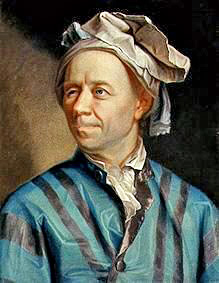
\includegraphics{EulerPortrait.jpg}
\caption{Leonhard Euler}
\end{figure}

The most basic numerical solution algorithm for differential equations
is Euler's method\footnote{Leonhard Euler was a brilliant 18th century
  Swiss mathematician who made many great advances in the theoretical
  and applied mathematics.}. Simply put, assuming we know the state of
the system at time $t$ and we wish to estimate the state of the system
at time $t+\Delta t$ (where $\Delta t$ is pronounced ``delta-t'' and
represents the change in time) we can use the following equation:

\[ \mathbf{y_{t+\Delta t}} = \mathbf{y_{t}} + \Delta t \times \mathbf{y'}(\mathbf{y_t}, t) \]

Let's walk through what this equation is doing. It first takes the
derivatives for the state variables at the current point in time. It
multiplies these rates of change by the $\Delta t$ (how far in the
future we want to know the results) and adds this change to the values
of the state variables at the starting point in time. The result is an
estimate of what the values in the future should be.

Let's now apply this to a concrete example. Start with our population
scenario, but instead of exponential growth we have a fixed inflow of
people at a rate of 20 per year. At $t=0$ we have 100 people and we want
to know the population in 10 years, using Euler's method we obtain the
following:

\[
\begin{aligned}
P_{10} &= P_0 + \Delta t \times \frac{dP}{dt} \\
&= P_0 + 10 \times 20 \\
&= 100 + 200 \\
&= 300
\end{aligned}
\]

Thus the population size in 10 years will be 300. In this simple
example, Euler's method works perfectly and generates the exact same
answer as we would have found using analytic solutions.

In general, however, we won't be so lucky. For most problems Euler's
method will generate results that contain some level of error compared
to what the true value should be. To see this let's explore our
exponential growth model again with an $\alpha$ of 0.1. As a reminder,
this model is:

\[ P(0) = 100 \] \[ \frac{dP}{dt} = 0.1 \times P \]

As we showed earlier, the precise solution to this model for $t=10$ (to
three decimal places) is 271.828. Let's see what we get using Euler's
method with $\Delta t = 10$. Carrying out similar calculations as before
we get:

\[
\begin{aligned}
P_{10} &= P_0 + \Delta t \times \frac{dP}{dt} \\
&= P_0 + 10 \times (0.1 \times P_0) \\
&= 100 + 10 \times (0.1 \times 100) \\
&= 100 + 10 \times 10 \\
&= 100 + 100 \\
&= 200
\end{aligned}
\]

So using Euler's method we obtain an estimate 200 for the population
size at $t=10$ when we know the true value should be around 272. That's
a pretty large error! Why does this error come about? Why do we so
significantly underestimate the final population size?

The reason is that we calculate the population's rate of change only at
$t=0$. For each of the ten years we are simulating, we assume the
population grows at the rate it would if there were exactly 100 people.
However, the population size is constantly increasing during these ten
years, so the rate at which it grows should also be increasing. Imagine,
the case of a bank account with an interest rate of 10\% yearly. The
bank account grows over time so the interest earned should also grow
from year to year. It's the same principle of compounding here.

How do we address this issue? Using Euler's method, we can do it simply
by changing how often we calculate the rates of change. In our previous
calculation, we went straight from $t=0$ to $t=10$ all in one step, we
used a $\Delta t$ in Euler's equation of 10. However, we could employ an
alternate calculation strategy where, for instance, we stepped from
$t=0$ to $t=5$, recalculated the derivative based on the new population
size and then stepped from $t=5$ to $t=10$. This would be equivalent to
used a $\Delta t$ of 5 and iterating the algorithm twice. Here is what
we get doing this:

\[
\begin{aligned}
P_{5} &= P_0 + \Delta t \times \frac{dP}{dt} \\
&= P_0 + 5 \times (0.1 \times P_0) \\
&= 100 + 50 \\
&= 150 \\
P_{10} &= P_5 + \Delta t \times \frac{dP}{dt} \\
&= P_5 + 5 \times (0.1 \times P_5) \\
&= 150 + 5 \times 15 \\
&= 150 + 75 \\
&= 225
\end{aligned}
\]

That result is certainly better, and we cut our error by over 33\%.
However, the error is still too large for most practical purposes. To
improve the numerical estimation even more, we can apply smaller and
smaller $\Delta t$'s. You probably have a good grasp of the calculations
now, so let's just show the results for each step of the simulation.
We'll look at $\Delta t = 2$ and $\Delta t = 1$.

\begin{longtable}[c]{@{}ll@{}}
\hline\noalign{\medskip}
$t$ & $P$
\\\noalign{\medskip}
\hline\noalign{\medskip}
0 & 100
\\\noalign{\medskip}
2 & 120
\\\noalign{\medskip}
4 & 144
\\\noalign{\medskip}
6 & 172.8
\\\noalign{\medskip}
8 & 207.4
\\\noalign{\medskip}
10 & 248.8
\\\noalign{\medskip}
\hline
\end{longtable}

\begin{longtable}[c]{@{}ll@{}}
\hline\noalign{\medskip}
$t$ & $P$
\\\noalign{\medskip}
\hline\noalign{\medskip}
0 & 100
\\\noalign{\medskip}
1 & 110
\\\noalign{\medskip}
2 & 121
\\\noalign{\medskip}
3 & 133.1
\\\noalign{\medskip}
4 & 146.4
\\\noalign{\medskip}
5 & 161.1
\\\noalign{\medskip}
6 & 177.2
\\\noalign{\medskip}
7 & 194.9
\\\noalign{\medskip}
8 & 214.4
\\\noalign{\medskip}
9 & 235.8
\\\noalign{\medskip}
10 & 259.4
\\\noalign{\medskip}
\hline
\end{longtable}

We see that as $\Delta t$ gets smaller and smaller our results become
more and more accurate. However, they are never perfect. There is always
some error. Even if we made $\Delta t$ as small as 0.1 (requiring 100
simulation steps), our final population size would be calculated to be
270, an error just under 1\%.

Figure 1 illustrates the application of Euler's method to numerically
estimate the trajectory for an example function. The smaller the
$\Delta t$'s in the estimation are, the better the results will be.
Other terms that can be used in place of $\Delta t$ are ``Step Size'',
``Time Step'' or just ``DT''. We prefer not to use the notation DT as it
is easily confusable with the $dt$ from differential equations. The
latter indicates an infinitesimally small change, while step sizes are
never infinitesimally small.

\begin{figure}[htbp]
\centering
\includegraphics{Euler.png}
\caption{Figure 1. Euler's method at work. The true trajectory for the
illustrative state variable is shown in green. Euler's method estimate
of this trajectory is shown in blue.}
\end{figure}

As you decrease the step size for the simulation, the results of the
simulation become more and more accurate\footnote{It is important to
  note at this point that when we discuss accuracies in this context we
  are specifically referring to models composed of continuous
  differential equations. If you are using agent based modeling or have
  discontinuities in your models -- which could occur if you use
  If-Then-Else logic -- then a smaller step size may not provide
  additional accuracy when there is some fundamental time step logic to
  the model.}. The cost of this increased accuracy, however, is
increased computation time. The computation time required by your model
is directly proportional to 1 over the step size. Thus, if you cut the
step size in half, your model will take twice as long to complete
simulating.

In general, you want a step size small enough that your results are
``accurate enough,'' but one that isn't so small that the simulation
takes too long to complete. A rule of thumb for choosing the step size
is to choose a starting step size that results in a fast simulation.
Then cut the value of the step size in half and simulate the model
again. If the results have not change materially between these two
simulations, keep the larger step size. If the results have changed, cut
the step size in half again and repeat until the results cease to
change.

\hyperdef{}{Ex-11-7}{\paragraph{}\label{Ex-11-7}}

\beginEx{Exercise 11-7}

Take the differential equation:

\[ P(0) = 20 \] \[ \frac{dP}{dt} = \frac{100}{P} \]

Given a step size of 1, find the values of $P$ at $t=0,1,2,3,4,5$ to one
decimal place using Euler's method.

\hfill{} \hyperref[Ans-11-7]{Answer Available}

\completeEx 

\hyperdef{}{Ex-11-8}{\paragraph{}\label{Ex-11-8}}

\beginEx{Exercise 11-8}

Take the differential equation:

\[ P(0) = 20 \] \[ \frac{dP}{dt} = P^2 - P \]

Given a step size of 1, find the values of $P$ at $t=0,1,2,3,4,5$ to one
decimal place using Euler's method.

\hfill{} \hyperref[Ans-11-8]{Answer Available}

\completeEx 

\subsection{Runge-Kutta Methods}

\begin{figure}[htbp]
\centering
\includegraphics{RungeKutta.png}
\caption{Carl Runge and Martin Kutta}
\end{figure}

Euler's method is not the only technique that can be used to numerically
solve differential equations. Another popular set of techniques are
called Runge-Kutta methods. Runge-Kutta methods are a family of
numerical differential equation solvers. In fact Euler's method itself
can be classified as a simple Runge-Kutta method.

One particular member of the Runge-Kutta family of methods that is
widely used is a 4th-order Runge-Kutta method. This method differs from
Euler's method in that for each step, it evaluates the model multiple
times and averages the resulting derivatives. Briefly, the driving set
of equations for this method is as follows:

\[
\begin{aligned}
\mathbf{y_{t+\Delta t}} &= \mathbf{y_{t}} + \Delta t \frac{\mathbf{a}+2 \times \mathbf{b}+2 \times \mathbf{c}+\mathbf{d}}{6} \\
\text{Where:} \\
\mathbf{a} &= \mathbf{y'}(\mathbf{y_t}, t) \\
\mathbf{b} &= \mathbf{y'}(\mathbf{y_t}+\frac{\Delta t}{2} \times \mathbf{a}, t+\frac{\Delta t}{2}) \\
\mathbf{c} &= \mathbf{y'}(\mathbf{y_t}+\frac{\Delta t}{2} \times \mathbf{b}, t+\frac{\Delta t}{2}) \\
\mathbf{d} &= \mathbf{y'}(\mathbf{y_t}+\Delta t \times \mathbf{c}, t+\Delta t) \\
\end{aligned}
\]

What this algorithm does is first compute the derivatives of the system
at the current time ($\mathbf{a}$) and use them to move the system
forward to $t+\Delta t/2$. The derivatives are evaluated at
$t+\Delta t/2$ ($\mathbf{b}$) and this new set of derivatives is used to
again move the system from $t$ to $t+\Delta t/2$. A third set of
derivatives are evaluated again at this mid-point ($\mathbf{c}$) and
they are the used to move the system from $t$ to $t+\Delta t$. A fourth
set of derivatives are evaluated at this point ($\mathbf{d}$). The
system is then returned to its starting point and a weighted average of
derivatives are used to move the system the full time step. This
weighting puts most of the weight on the middle two derivatives instead
of the derivatives from the end points.

This 4th-order Runge-Kutta method is generally much more accurate than
Euler's method for a given step size. Using a step size of 10 for our
earlier population model, the Runge-Kutta method generates a value of
270.8. A step size of 5 yields a results of 271.7, just a smidgeon away
from the precise value of 271.8. Recall that for Euler's method, even
with a step size of 0.1 we still were not as accurate as the Runge-Kutta
method with a step size of 5. Now it is true that this 4th-Order
Runge-Kutta method does a lot more work than Euler's method for each
step. It evaluates the model for times and has to do some averaging of
derivatives. However, it is still much more accurate than Euler's method
for an equivalent level of computational effort.

\hyperdef{}{Ex-11-9}{\paragraph{}\label{Ex-11-9}}

\beginEx{Exercise 11-9}

Take the differential equation:

\[ P(0) = 20 \] \[ \frac{dP}{dt} = \frac{100}{P} \]

Given a step size of 1, find the values of $P$ at $t=0,1,2,3,4,5$ to one
decimal place using the 4th-Order Runge-Kutta method.

\hfill{} \hyperref[Ans-11-9]{Answer Available}

\completeEx 

\hyperdef{}{Ex-11-10}{\paragraph{}\label{Ex-11-10}}

\beginEx{Exercise 11-10}

Take the differential equation:

\[ P(0) = 20 \] \[ \frac{dP}{dt} = P^2 - P \]

Given a step size of 1, find the values of $P$ at $t=0,1,2,3,4,5$ to one
decimal place using the 4th-Order Runge-Kutta method.

\hfill{} \hyperref[Ans-11-10]{Answer Available}

\completeEx 

\paragraph{}

\beginEx{Exercise 11-11}

Discuss the differences between the 4th-Order Runge Kutta solutions and
the Euler solutions. What causes these differences? Which method is most
accurate? Why?

\completeEx 

\paragraph{}

\beginEx{Exercise 11-12}

Describe a model where Euler's method would be best suited as a
numerical solver. Describe a model where the 4th-Order Runge-Kutta
method would be best suited.

\completeEx 

\FloatBarrier 

\begin{model}[frametitle={Model: Numerical Solution Algorithms}] 

 This model explores the selection of the simulation step size and differential equation solution algorithm.





\begin{enumerate}[label=\protect\circled{\arabic*}] \setcounter{enumi}{0}

\item Create a new \a{Stock} named \p{Population}.


\item  Change the \a{Initial Value} property of the primitive \p{Population} to \e{100}.


\item Create a new \a{Flow} going from empty space to the primitive \p{Population}. Name that flow \p{Net Growth}.


\item Create a new \a{Variable} named \p{Growth Rate}.


\item  Change the \a{Equation} property of the primitive \p{Growth Rate} to \e{0.1}.


\item Create a new \a{Link} going from the primitive \p{Growth Rate} to the primitive \p{Net Growth}.


\item  Change the \a{Flow Rate} property of the primitive \p{Net Growth} to \e{[Growth Rate]*[Population]}.


\item Create a new \a{Variable} named \p{True Population}.


\item Create a new \a{Link} going from the primitive \p{Growth Rate} to the primitive \p{True Population}.


\item  Change the \a{Equation} property of the primitive \p{True Population} to \e{100*Exp([Growth Rate]*Years)}.


\item  Change the \a{Simulation Length} property of the Time Settings to \e{10}.


\item The model diagram should now look something like this: \par \begin{minipage}{\linewidth}  \centering \includegraphics{model_35/diagram_13.png}
\end{minipage}




\end{enumerate} 



Let's now implement the simple exponential growth model we have discussed in this chapter. We have a population that starts with 100 people and increases at a rate of 10\% per year. In addition to creating the stock and flow model, we have also created a variable, \p{True Population}, that contains the analytical solution to the model.







First, we'll use Euler's method with a step size of 2 years and simulate the model.





\begin{enumerate}[label=\protect\circled{\arabic*}] \setcounter{enumi}{12}

\item  Change the \a{Simulation Time Step} property of the Time Settings to \e{2}.


\item Run the model. Here are sample results:\par \begin{minipage}{\linewidth}  \centering \includegraphics{model_35/result_17.png}
\end{minipage}




\end{enumerate} 



As we can see these results aren't very accurate. The value of the numerical estimated \p{Population} is quite different from the analytically determined value in \p{True Population}. Let's reduce the step size to 1 year and try again.





\begin{enumerate}[label=\protect\circled{\arabic*}] \setcounter{enumi}{14}

\item  Change the \a{Simulation Time Step} property of the Time Settings to \e{1}.


\item Run the model. Here are sample results:\par \begin{minipage}{\linewidth}  \centering \includegraphics{model_35/result_20.png}
\end{minipage}




\end{enumerate} 



This is better, but we're still off by a fair amount. We could experiment with continuing to reduce the step size, but let's instead switch now to the more accurate Runge-Kutta method. Will simulate the model again with a step size of 1 using the 4th-Order Runge-Kutta solution algorithm.





\begin{enumerate}[label=\protect\circled{\arabic*}] \setcounter{enumi}{16}

\item  Change the \a{Analysis Algorithm} property of the Time Settings to \e{RK4}.


\item Run the model. Here are sample results:\par \begin{minipage}{\linewidth}  \centering \includegraphics{model_35/result_23.png}
\end{minipage}




\end{enumerate} 



That's a lot better! It's so close to being perfect that we can’t even see the difference between the two lines in the figure. Just to be clear, let's see how quickly the results degrade when we increase the step size. Let's set the step size to 10 and simulate the model again.





\begin{enumerate}[label=\protect\circled{\arabic*}] \setcounter{enumi}{18}

\item  Change the \a{Simulation Time Step} property of the Time Settings to \e{10}.


\item Run the model. Here are sample results:\par \begin{minipage}{\linewidth}  \centering \includegraphics{model_35/result_26.png}
\end{minipage}




\end{enumerate} 



That's still very good and much better than Euler's Method with a step size of 1. Why don't you go ahead now and experiment with different step sizes and the two solution methods to get a feel for their accuracies.




 \end{model}

\subsection{Other Solution Techniques}

While being a brief introduction into numerical solution methods for
differential equations, this should provide you with the background you
need to intelligently make decisions about controlling the simulation of
your models. It should help you identify potential sources of errors in
your model and help you to adjust you simulation configuration to
account for them.

The two methods we have looked at for solving differential equation
models -- Euler's method and a 4th-Order Runge-Kutta method -- are
widely used and they are what are built into Insight Maker. In addition
to these two techniques, however, there are many other methods that are
used in practice and you should be aware of this richer ecosystem of
solution techniques.

Although we do not have space here to delve into the full ecosystem of
numerical differential equation algorithms, it is useful to discuss one
variant briefly: the adaptive step size algorithm. The methods we have
looked at here use a fixed step size specified at the beginning of a
simulation. Many models, however, might be characterized by highly
variable trajectories. Part of the trajectory might be very smooth and
unchanging while other parts might experience numerous rapid changes.

When using a fixed step size algorithm like the ones illustrated above,
the step size must be set for the worse case scenario. The step size
must be set to a small enough value to account for the rapidly changing
areas. That said, the precision of this small step size is unnecessary
on the smooth regions of the trajectory where the algorithm must do
extra work for minimal gain in precision. Ideally, we would want to have
a small step size for the rapidly changing areas and a large one for the
smooth regions. This would result in the best of both worlds: high
accuracy and quick computation.

\begin{figure}[htbp]
\centering
\includegraphics{Adaptive.png}
\caption{Figure 2. Illustration of an adaptive step size algorithm. Dots
show the location of model evaluations. Evaluations are clustered around
changes in the derivatives.}
\end{figure}

Adaptive step size algorithms do just that. They adjust the step size
dynamically based on the behavior of the model's derivatives. If the
derivatives change rapidly, then the step size will be automatically
shrunk; if the derivatives are constant or change very slowly the step
size will automatically grow. Figure 2 illustrates the location of steps
for an illustrative model using an adaptive step size algorithm. The
steps are clustered around changes in the trajectory's derivatives in an
attempt to maximize predictive accuracy while minimizing computation
effort.

\chapter{Equilibria and Stability Analysis}

This chapter extends on our mathematical analysis of models by
introducing the concepts of points of equilibria and stability analysis.
These types of analyses allow you to determine many behaviors of a
system without needing to fully solving its differential equation model.

Although the trajectory for the state variables in differential equation
models generally cannot be determined analytically, several key
properties of models can often still be determined. These properties
include:

\begin{itemize}
\itemsep1pt\parskip0pt\parsep0pt
\item
  The location of equilibrium points
\item
  The stability of the equilibrium points
\end{itemize}

An equilibrium point is defined as a set of state variable values that
will cause the system to cease to change. Once the system enters an
equilibrium configuration, it will not leave that configuration without
an external stimulus. For instance, in our exponential growth model a
single equilibrium point exists: that of zero people. If the population
is empty, then the population will not grow and instead remain at 0
indefinitely.

In the exponential growth population model there is only one equilibrium
point ($P=0$). In other models you may have multiple equilibrium points.
In a model of a highly infectious, incurable disease you can imagine a
system where two equilibrium points exist: one where no one is infected
and a second point where everyone is infected. As long as there were no
infectious individuals, the population would remain healthy. If just a
single infected individual were introduced into the population, the
infection would, however, spread until everyone was infected and the
population would then remain at that point (remember this hypothetical
disease is incurable).

Multiple types of equilibria exist. Figure 1 illustrates what is known
as the \emph{stability} of equilibrium points. Each of the three panes
in this figure show a different form of equilibrium for the ball. In all
three the balls are in equilibrium: if the no external forces come into
play, the balls will not move. What differs in each of the three is what
occurs if the balls are displaced a small amount.

\begin{figure}[htbp]
\centering
\includegraphics{Stability.png}
\caption{Figure 1. Three different types of stability.}
\end{figure}

Stable Equilibrium : In this type of equilibrium the ball will return to
its original position if it is displaced. The structure of the system is
such that the system is naturally attracted to the point of equilibrium.
To use the physical metaphor, the equilibrium is at the bottom of a dip
and the system naturally rolls into it.

Unstable Equilibrium : Here the ball will move further and further away
from the point of equilibrium if it is displaced even a small amount.
The equilibrium is unstable in that if we are just a small distance away
from it, we move further away from it. To use the physical metaphor, the
equilibrium is at the top of the hill and the system will move away from
it unless it is placed at the exact point of equilibrium.

``Neutrally Stable Equilibrium'' : This is a less common form of
equilibrium and goes by several different names. In this case if the
ball is moved it will stay fixed at its new location. It will not move
closer to or further from the original equilibrium. Of the three types
of equilibrium, this one is less interest or relevance in practice.

In the case of the highly infectious disease model, an equilibrium of
everyone being healthy would be classified as an unstable equilibrium.
The equilibrium would persist as long as no one brought the disease into
the population (someone would not just spontaneously become ill), but if
as little as a single sick person entered the population, the population
would move further and further away from the equilibrium point of
everyone being healthy and would never naturally return to it.

The equilibrium point of everyone being sick is, on the other hand, a
stable equilibrium as no one recovers from the disease on their own.
Even if you introduced healthy people into a population of sick
individuals -- moving the population away from the equilibrium -- they
too will eventually become sick restoring the population to the
equilibrium of everyone being sick.

\hyperdef{}{Ex-12-1}{\paragraph{}\label{Ex-12-1}}

\beginEx{Exercise 12-1}

Provide two examples each of situations where stable and unstable
equilibria occur in nature. Describe these equilibria.

\hfill{} \hyperref[Ans-12-1]{Answer Available}

\completeEx 

\section{Equilibrium Points}

Often, we can determine the equilibrium points for a system without
fully needing to solve the trajectory for the state variables. Let's
implement the simple disease model we've been discussing. We'll do so
for both a differential equation model and a System Dynamics model, but
we'll rely on differential equation version to do our analytic analysis.

One way to express the differential version of the model is to define
two state variables: the number of healthy people ($H$) and the number
of sick people ($S$). The rate of infection between sick and healthy
people can be made a function of the number of people in each category.
Clearly, if there are no sick people the infection rate is 0; but, just
as clearly, if everyone is already sick then the infection rate will
also be zero. One workable differential equation model to implement this
behavior is shown below:

\[
\begin{aligned}
H(0) &= 100 \\
S(0) &= 1 \\
\frac{dH}{dt} &= - \alpha \times H \times S \\ 
\frac{dS}{dt} &= \alpha \times H \times S
\end{aligned}
\]

This model uses a single parameter ($\alpha$) to control the infection
rate. $alpha$ is a non-zero positive value; the smaller $\alpha$ is, the
slower the infection will progress and vice versa. This notation
illustrates one of the clumsier aspects of implementing stock and flow
models using differential equations. The flow values between two stocks
have to be repeated twice once for each of the two connected state
variable's derivatives.

\FloatBarrier 

\begin{model}[frametitle={Model: Incurable Disease}] 

 This model illustrates stable and unstable equilibria using the scenario of an incurable disease in a population.





\begin{enumerate}[label=\protect\circled{\arabic*}] \setcounter{enumi}{0}

\item Create a new \a{Stock} named \p{Healthy}.


\item Create a new \a{Stock} named \p{Sick}.


\item Create a new \a{Flow} going from the primitive \p{Healthy} to the primitive \p{Sick}. Name that flow \p{Infection}.


\item Create a new \a{Variable} named \p{Infection Rate}.


\item Create a new \a{Link} going from the primitive \p{Infection Rate} to the primitive \p{Infection}.


\item The model diagram should now look something like this: \par \begin{minipage}{\linewidth}  \centering \includegraphics{model_36/diagram_7.png}
\end{minipage}




\end{enumerate} 



This is the structure of our model. We have two stocks of people with people moving from the healthy stock to the sick stock as they become infected. Let's add the values and equations now.





\begin{enumerate}[label=\protect\circled{\arabic*}] \setcounter{enumi}{6}

\item  Change the \a{Initial Value} property of the primitive \p{Healthy} to \e{100}.


\item  Change the \a{Initial Value} property of the primitive \p{Sick} to \e{0}.


\item  Change the \a{Equation} property of the primitive \p{Infection Rate} to \e{0.01}.


\item  Change the \a{Flow Rate} property of the primitive \p{Infection} to \e{[Infection Rate]*[Healthy]*[Sick]}.


\end{enumerate} 



There our model is fully setup. We've set it to start with everyone being healthy.





\begin{enumerate}[label=\protect\circled{\arabic*}] \setcounter{enumi}{10}

\item Run the model. Here are sample results:\par \begin{minipage}{\linewidth}  \centering \includegraphics{model_36/result_15.png}
\end{minipage}




\end{enumerate} 



These results are quite stable. Everyone is healthy and no one gets sick. That indicates we have an equilibrium here. Let's now experiment by making a single person in the population sick.





\begin{enumerate}[label=\protect\circled{\arabic*}] \setcounter{enumi}{11}

\item  Change the \a{Initial Value} property of the primitive \p{Sick} to \e{1}.


\item  Change the \a{Initial Value} property of the primitive \p{Healthy} to \e{99}.


\item Run the model. Here are sample results:\par \begin{minipage}{\linewidth}  \centering \includegraphics{model_36/result_19.png}
\end{minipage}




\end{enumerate} 



That's more interesting! We can see that everyone being healthy is an unstable equilibrium as the system moves away from it if we deviate from it by even a small amount. We can also see that the second equilibrium (everyone being sick) is stable as the system moves towards it naturally.




 \end{model}

Finding the equilibria for differential equation models is by-and-large
straightforward analytically. We simply need to harness the definition
of an equilibrium point: an equilibrium point is one where the state
variables are constant and unchanging. Since the derivatives represent
changes in the state variables, this statement is equivalent to saying
the derivatives for the model are 0 at equilibrium points.

Based on this, in order to find the equilibrium points we simply need to
set the derivatives in our model to 0 and solve the resulting equations.
For the disease model we get:

\[
\begin{aligned}
H(0) = 99 \\
S(0) = 1 \\
0 = - \alpha \times H \times S \\ 
0 = \alpha \times H \times S
\end{aligned}
\]

The initial conditions will determine what equilibrium is arrived at but
they do not affect the existence of the equilibria. Furthermore, the two
equations we have set to 0 are equivalent\footnote{Although we expressed
  this model as a function of two state variables $H$ and $S$, it only
  has one independent state variable. Given the fixed population size,
  you know the value of $H$ given $S$ and vice versa.} so we can
simplify these equations to simply be:

\[ 
0 = \alpha \times H \times S
\]

Simple inspection reveals that this equation is true if and only if
either $H=0$, $S=0$, or $\alpha=0$. Thus we have mathematically shown
that our equilibria are either when everyone is sick or everyone is
healthy (or there is no infection whatsoever). Granted this is a trivial
conclusion for this model and we stated it earlier. However, for more
complex models this type of analysis can be very useful and will often
reveal that equilibria are functions of the different parameter values
in the model and they may enable you to explicitly determine how the
equilibria changes as the model configuration changes.

Let's try a more complex example. Remember the predator prey model from
earlier? We had the following set of equations to simulate the
relationship between a moose and wolf population:

\[ \frac{dM}{dt} = \alpha \times M - \beta \times M \times W \]
\[ \frac{dW}{dt} = \gamma \times M \times W - \delta \times W  \]

Let's determine what the equilibrium values are for this model. As
before, we start by setting the derivatives to 0:

\[ 0 = \alpha \times M - \beta \times M \times W \]
\[ 0 = \gamma \times M \times W - \delta \times W \]

Solving this set of equations is more difficult than for the disease
model. However a little bit of algebra reveals two solutions. One when
$M=0$ and $W=0$ (there are no animals at all), and the second when
$M=\delta/\gamma$ and $W=\alpha/\beta$. This is an example of where the
equilibrium location depends on the values of the model parameters.

\hyperdef{}{Ex-12-2}{\paragraph{}\label{Ex-12-2}}

\beginEx{Exercise 12-2}

Find the equilibrium points for the system:

\[ \frac{dX}{dt} = X^2+X-3\]

\hfill{} \hyperref[Ans-12-2]{Answer Available}

\completeEx 

\hyperdef{}{Ex-12-3}{\paragraph{}\label{Ex-12-3}}

\beginEx{Exercise 12-3}

Find the equilibrium points for the system:

\[ \frac{dX}{dt} = \sin(X)\]

\hfill{} \hyperref[Ans-12-3]{Answer Available}

\completeEx 

\hyperdef{}{Ex-12-4}{\paragraph{}\label{Ex-12-4}}

\beginEx{Exercise 12-4}

Find the equilibrium points for the system:

\[
\begin{aligned}
\frac{dX}{dt} = 2 \times X + Y + 5\\
\frac{dY}{dt} = 3 \times X - 4 \times Y
\end{aligned}
\]

\hfill{} \hyperref[Ans-12-4]{Answer Available}

\completeEx 

\hyperdef{}{Ex-12-5}{\paragraph{}\label{Ex-12-5}}

\beginEx{Exercise 12-5}

Find the equilibrium points for the system:

\[
\begin{aligned}
\frac{dX}{dt} &= X^2 - Y \\
\frac{dY}{dt} &= -2 \times X^2 - Y^2
\end{aligned}
\]

\hfill{} \hyperref[Ans-12-5]{Answer Available}

\completeEx 

\paragraph{}

\beginEx{Exercise 12-6}

Do the locations of equilibria depend on the starting conditions? Does
the system arriving at an equilibrium depend on the starting conditions?

Why or why not?

\completeEx 

\section{The Phase Plane}

Up until now, when looking at model results we have been focused on time
series plots and we have mainly been interested in the trajectory of the
variables and stocks over time. For the mathematical analysis of
differential equations, however, the primary graphical tool is not this
time series plot; instead it is what is known as a phase plane plot.

Phase planes are almost like scatterplots. They show one of the state
variables plotted against another of the state variables. A scatterplot
could be used to show the path for these two variables over the course
of a simulation. In the predator prey model the results of a scatterplot
of the wolf and moose population will be an ellipsoid. The two
populations will cycle continuously. A phase plane plot is similar to
this, but rather than just showing one of these cycles for a given
simulation run, the phase plane shows the trajectories for \emph{all}
combinations of moose and wolf population sizes.

\begin{figure}[htbp]
\centering
\includegraphics{PredatorPreyPhasePlane.png}
\caption{Figure 2. Predator prey phase plane plot. The trajectory for a
single set of initial conditions is highlighted in red.}
\end{figure}

Figure 2 illustrates a phase plane plot for the predator prey system.
The trajectory for one set of parameter and state variable values is
highlighted in red and, as expected, we see a continual oscillation. We
can also see the trajectories for all the other combinations of state
variables. We see that the system will always oscillate and the size of
this oscillation depends on the initial conditions for the state
variables. This illustration provides us with a good deal of information
in a single graphic and the phase plane plot is a great way to summarize
the behavior of a system with two state variables.

Let's quickly explore the phase plane plots for a simpler system than
our predator prey model. Take a system consisting of two state
variables\footnote{Just a helpful reminder if you are starting to get
  lost in some of this differential equation jargon. A ``state
  variable'' is just a stock. Return to the table at the beginning of
  this chapter to see how these terms relate to the system dynamics
  modeling terminology we have already learned.} both of which grow (or
decay) exponentially. These state variables will be assumed to be
independent from each other so the value of one does not affect the
value of the other:

\[
\begin{aligned}
\frac{dX}{dt} &= \alpha \times X \\
\frac{dY}{dt} &= \beta \times Y \\
\end{aligned}
\]

Clearly, there is an equilibrium point for this model at $X=0$ and
$Y=0$. There are four general types of behavior around this equilibrium.
One when $\alpha>0$ and $\beta>0$, one when $\alpha<0$ and $\beta>0$,
one when $\alpha>0$ and $\beta<0$, and one when $\alpha<0$ and
$\beta<0$. The phase planes for each of the four cases are shown in
Figure 3.

\begin{figure}[htbp]
\centering
\includegraphics{SimplePhasePlanes.png}
\caption{Figure 3. Phase planes for a simple two state variable
exponential growth model.}
\end{figure}

From these plots we can visually determine how the stability of the
equilibrium point at $X=0, Y=0$ changes as we change $\alpha$ and
$\beta$. When $\alpha<0$ and $\beta<0$, we have a stable equilibrium; in
all other cases we have an unstable equilibrium.

\paragraph{}

\beginEx{Exercise 12-7}

Sketch out the phase plane for the differential equation model:

\[
\begin{aligned}
\frac{dX}{dt} &=  -1 \\
\frac{dY}{dt} &= Y \\
\end{aligned}
\]

\completeEx 

\paragraph{}

\beginEx{Exercise 12-8}

Sketch out the phase plane for the differential equation model:

\[
\begin{aligned}
\frac{dX}{dt} &=  X \\
\frac{dY}{dt} &= Y^2 \\
\end{aligned}
\]

\completeEx 

\section{Stability Analysis}

Now that we have learned how to analytically determine the location of
equilibrium points, we may want to determine what type of stability
occurs at these equilibria. As we stated earlier, for the incurable
disease model it is trivial to arrive at the conclusion that the state
of everyone being healthy is unstable while the state of everyone being
sick is stable. In more complex models, it may be harder to draw
conclusions or the stability of an equilibrium point may change as a
function of the model's parameter values. Fortunately, there is a
general way to determine the precise stability nature of the equilibrium
points analytically.

The procedure to do this is relatively straightforward, but the theory
behind it can be difficult to understand. The first key principle that
must be understood is that of ``linearization''. To get a feel for
linearization, let's take the curve in Figure 4. Clearly this curve is
not linear. It has lots of bends and does not look at all like a line.

\begin{figure}[htbp]
\centering
\includegraphics{Linearization.png}
\caption{Figure 4. As we zoom in on a function it becomes more and more
linear.}
\end{figure}

If we zoom in on any one part of the curve, however, the section we are
zoomed in on starts to straighten out. If we keep zooming in, we will
eventually reach a point where the section we are zoomed in on is
effectively linear: basically a straight line. This is true for whatever
part of the curve we zoom in on\footnote{The one exception to this rule
  is if your curve is some sort of fractal. In this case no matter how
  much you zoom in on it, it will never become straight. In practice,
  however, this caveat is a non-issue.}. The more bendy parts of the
curve will just take more zooming to convert them to a line.

We can conceptually do the same process for the equilibrium points in
our phase planes. Even if the trajectories of the state variables in the
phase planes are very curvy, if we zoom in enough on the equilibrium
points, the trajectories at a point will eventually become effectively
linear. The simple, two-state variable exponential growth model we
illustrated with phase planes above are examples of a fully linear
model. If we zoom in sufficiently on the equilibrium points for most
models, the phase planes for the zoomed-in version of the model will
eventually start to look like one of these linear cases.

Mathematically, we apply linearization to an arbitrary model by first
calculating what is called the Jacobian matrix of the model. The
Jacobian matrix is the matrix of partial derivatives of each of
derivatives in the model with respect to each of the state variables:

\[ \text{Jacobian} = \begin{bmatrix} \dfrac{\partial }{\partial X} X' & \cdots & \dfrac{\partial }{\partial Z} X' \\ \vdots & \ddots & \vdots \\ \dfrac{\partial }{\partial X} Z' & \cdots & \dfrac{\partial }{\partial Z} Z'  \end{bmatrix} \]

The Jacobian is a linear approximation of our (potentially) non-linear
model derivatives. Let's take the Jacobian matrix for the simple
exponential growth model:

\[
\begin{aligned}
\frac{dX}{dt} &= \alpha \times X \\
\frac{dY}{dt} &= \beta \times Y \\
\end{aligned}
\]

\[
\begin{aligned}
\text{Jacobian} &= \begin{bmatrix} \dfrac{\partial}{\partial X } \alpha \times X & \dfrac{\partial}{\partial Y } \alpha \times X  \\  \dfrac{\partial}{\partial X } \beta \times Y & \dfrac{\partial}{\partial Y } \beta \times Y \end{bmatrix}
&= \begin{bmatrix} \alpha  & 0 \\ 0 & \beta \end{bmatrix}
\end{aligned}
\]

\hyperdef{}{Ex-12-9}{\paragraph{}\label{Ex-12-9}}

\beginEx{Exercise 12-9}

Calculate the Jacobian matrix of the system:

\[
\begin{aligned}
\frac{dX}{dt} &=  X \\
\frac{dY}{dt} &= Y^2 \\
\end{aligned}
\]

\hfill{} \hyperref[Ans-12-9]{Answer Available}

\completeEx 

\hyperdef{}{Ex-12-10}{\paragraph{}\label{Ex-12-10}}

\beginEx{Exercise 12-10}

Calculate the Jacobian matrix of the system:

\[
\begin{aligned}
\frac{dX}{dt} &= X^2 - Y \\
\frac{dY}{dt} &= -2 \times X^2 - Y^2
\end{aligned}
\]

\hfill{} \hyperref[Ans-12-10]{Answer Available}

\completeEx 

\hyperdef{}{Ex-12-11}{\paragraph{}\label{Ex-12-11}}

\beginEx{Exercise 12-11}

Calculate the Jacobian matrix of the system:

\[
\begin{aligned}
\frac{dX}{dt} &= X \times Y + \beta \times Y^2 \\
\frac{dY}{dt} &= \alpha \times X^3 + X^2 \times Y
\end{aligned}
\]

\hfill{} \hyperref[Ans-12-11]{Answer Available}

\completeEx 

This is complicated so don't worry if you don't completely understand
it! Once you have the Jacobian, you calculate what are known as the
eigenvalues of the Jacobian at the equilibrium points. This is also a
bit complicated, so if your head is starting to spin, just skip forward
in this chapter!

Nonetheless, eigenvalues and their sibling eigenvectors are an
interesting subject. Given a square matrix (a matrix where the number of
rows in equals the number of columns), an eigenvector is a vector which,
when multiplied by the matrix, results is the original vector multiplied
by some factor. This factor is known as an eigenvalue as is usually
denoted $\lambda$. Given a matrix $\mathbf{A}$, an eigenvalue $\lambda$
with associated eigenvector $\mathbf{V}$; the following equation will be
true:

\[\mathbf{A} \times \mathbf{V} = \lambda \times \mathbf{V}\]

Let's look at an example for a $2\times2$ matrix:

\[\begin{bmatrix} 1 & 2 \\ 1 & 0 \end{bmatrix} \times \mathbf{V} = \lambda \times \mathbf{V}\]

What eigenvector and eigenvalue combinations satisfy this equation? It
turns out there are two key ones:

\[\begin{bmatrix} 1 & 2 \\ 1 & 0 \end{bmatrix} \times \begin{bmatrix} 2 \\ 1 \end{bmatrix}= 2 \times \begin{bmatrix} 2 \\ 1 \end{bmatrix}\]

\[\begin{bmatrix} 1 & 2 \\ 1 & 0 \end{bmatrix} \times \begin{bmatrix} -1 \\ 1 \end{bmatrix} = -1 \times \begin{bmatrix} -1 \\ 1 \end{bmatrix}\]

Naturally, any multiple of an eigenvector will also be an eigenvector.
For instance, in the case above, $[1, 0.5]$ and $[-2, 2]$ are also
eigenvectors of the matrix.

We can interpret eigenvectors geometrically. Looking at the $2\times2$
matrix case, we can think of a vector as representing a coordinate in a
two-dimensional plane: $[x,y]$. When we multiply our $2\times2$ matrix
by the point, we transform the point into another point also in the
two-dimensional plane. Due to the properties of eigenvectors, we know
that when we transform an eigenvector, the transformed point will just
be a multiple of the original point. Thus when a point that is on a
matrix's eigenvector is transformed by that matrix, it will move inwards
or outwards from the origin along the line defined by the matrix's
eigenvector.

We can now relate the concept of eigenvalues and eigenvectors to our
differential equation models. Take a look back at the phase planes for
the exponential model example. For each of the phase planes, there are
at least two straight lines of trajectories. In these cases the
\emph{x}- axis and the \emph{y}-axis are the locations of these
trajectories. If you have a system on the \emph{x}- or \emph{y}-axis in
this example it will remain on that axis as it changes. This indicates
that for this model, the eigenvectors are the two axises as a system on
either of them does not change direction as it develops. That's the
definition of of an eigenvector.

For our purposes though, we do not really care about the actual
direction or angle for these eigenvectors. We instead care about whether
the state variables move inwards or outwards along these vectors. We can
determine this from the eigenvalues of the Jacobian matrix. If the
eigenvalue for an eigenvector is negative, then the values move inwards
along that eigenvector; while if the eigenvalue is positive, they move
outward along the eigenvector.

These eigenvalues tell us all we need to know about the stability of the
system. Returning to our illustration of stability as a ball on a hill,
we can think of these eigenvalues as being the slopes of the hill around
the equilibrium point. If the eigenvalues are negative, the ground
slopes down towards the equilibrium point forming a cup (leading to a
stable equilibrium). If the eigenvalues are positive, the ground slopes
away from the equilibrium point creating a hill (leading to an unstable
equilibrium).

Eigenvalues can be calculated straightforwardly for a given Jacobian
matrix. Briefly, for the Jacobian matrix $J$, the eigenvalues $\lambda$
are the values that satisfy the following equation where $det$ is the
matrix determinant and $I$ is the identity matrix.

\[
0=det(J-\lambda \times I)
\]

We can do a quick example of calculating the eigenvalues for the
Jacobian matrix we derived for our two-state variable exponential growth
model.

\[
\begin{aligned}
0 &= det\left(\begin{bmatrix} \alpha  & 0 \\ 0 & \beta \end{bmatrix} - \lambda  \times  \begin{bmatrix} 1 & 0 \\ 0 & 1 \end{bmatrix} \right) \\
 &= det\left(\begin{bmatrix} \alpha -\lambda & 0 \\ 0 & \beta-\lambda \end{bmatrix}\right) \\
 &= (\alpha-\lambda) \times (\beta-\lambda) - 0 \times 0 \\
\lambda = \alpha, \lambda = \beta
\end{aligned}
\]

That is a fair amount of work to do. It's even more complicated if you
have more than two state variables. However, once you have gone through
the calculations and determined the linearized eigenvalues for your
equilibrium points, you know everything you might want to know about the
stability of the system.

\hyperdef{}{Ex-12-12}{\paragraph{}\label{Ex-12-12}}

\beginEx{Exercise 12-12}

Find the eigenvalues of the following matrix:

\[
\begin{bmatrix} 2 & 4 \\  4 & 2 \end{bmatrix}
\]

(Bonus: Determine the associated eigenvectors.)

\hfill{} \hyperref[Ans-12-12]{Answer Available}

\completeEx 

\hyperdef{}{Ex-12-13}{\paragraph{}\label{Ex-12-13}}

\beginEx{Exercise 12-13}

Find the eigenvalues of the following matrix:

\[
\begin{bmatrix} 2 & 0 \\  5 & 1 \end{bmatrix}
\]

(Bonus: Determine the associated eigenvectors.)

\hfill{} \hyperref[Ans-12-13]{Answer Available}

\completeEx 

\hyperdef{}{Ex-12-14}{\paragraph{}\label{Ex-12-14}}

\beginEx{Exercise 12-14}

Find the eigenvalues of the following matrix:

\[
\begin{bmatrix} \alpha & \beta \\  \beta & \alpha \end{bmatrix}
\]

(Bonus: Determine the associated eigenvectors.)

\hfill{} \hyperref[Ans-12-14]{Answer Available}

\completeEx 

\hyperdef{}{Ex-12-15}{\paragraph{}\label{Ex-12-15}}

\beginEx{Exercise 12-15}

\[
\begin{bmatrix} \alpha & \beta \\  0 & \beta \end{bmatrix}
\]

(Bonus: Determine the associated eigenvectors.)

\hfill{} \hyperref[Ans-12-15]{Answer Available}

\completeEx 

In the exponential growth model we can see that when the eigenvalues are
both negative we have a stable equilibrium (refer to the graphs we
developed earlier), while if either one is positive (or they both are)
we have an unstable equilibrium. This makes a lot of sense as if either
one is positive it pushes the system away from the equilibrium making it
unstable. While if they are both negative then they both push the system
towards the equilibrium point. Visualize the ball sitting in the cup or
on the hill.

Looking at it this way, we realize that \emph{all we need in order to
understand the stability of an equilibrium point are the eigenvalues of
the Jacobian at the equilibrium point}. This is an incredibly powerful
tool. It reduces the complex concept of stability, into an analytical
procedure that can be applied straightforwardly.

Let's now look at some more examples.

First let's take our simple disease model from earlier. If you recall
that model was:

\[
\begin{aligned}
\frac{dH}{dt} &= - \alpha \times H \times S \\ 
\frac{dS}{dt} &= \alpha \times H \times S
\end{aligned}
\]

First let's calculate the Jacobian for this model. We take the partial
derivatives of each of the two derivatives with respect to each of the
two state variables to create a two-by-two matrix:

\[
\text{Jacobian} = \begin{bmatrix} \dfrac{\partial}{\partial H }  - \alpha \times H \times S& \dfrac{\partial}{\partial S }  - \alpha \times H \times S  \\  \dfrac{\partial}{\partial H } \alpha \times H \times S & \dfrac{\partial}{\partial S } \alpha \times H \times S \end{bmatrix} =\begin{bmatrix}
-\alpha \times S & -\alpha \times H \\
\alpha \times S & \alpha \times H
\end{bmatrix}
\]

Next, we evaluate this Jacobian at one of our equilibrium points. Let's
choose the one where the $S=0$ (no one is sick) and $H=P$ (where $P$ is
the population size) so everyone is healthy:

\[
\begin{bmatrix}
0 & -\alpha \times P \\
0 & \alpha \times P
\end{bmatrix}
\]

We can now find the eigenvalues for this matrix. Once we go through the
math we get two eigenvalues: 0 and $\alpha \times P$. What do these
mean? Well, since one of the eigenvalues is positive, this indicates we
have movement away from the equilibrium point along at least one of the
eigenvectors. The other vector has no movement (0 as the eigenvalue),
but this one positive value will ensure we have an unstable equilibrium.
Again, think of the ball, the positive eigenvalue indicates the ground
slopes downwards from the equilibrium point so a ball balanced on top of
this hill will be very unstable.

Now let's do the second equilibrium. The one where $S=P$ and $H=0$
(everyone is sick). Let's evaluate the Jacobian at this equilibrium:

\[
\begin{bmatrix}
-\alpha \times P & 0 \\
\alpha \times P & 0
\end{bmatrix}
\]

Now let's find the eigenvalues for this matrix. Once we go through the
math we get two eigenvalues: this time 0 and $-\alpha \times P$. Again,
the 0 eigenvalue can be ignored as it does not cause growth or change.
The second eigenvalue however is negative, indicating the system moves
toward the equilibrium point again. Look back at our exponential growth
phase planes. Negative coefficients indicate trajectories towards the
equilibrium (create a cup for the ball). Thus this second equilibrium is
a stable one.

It's time to look at a more complex example, we'll consider our predator
prey model. First we calculate the Jacobian matrix for this model:

\[
\begin{split}
\text{Jacobian} &= \begin{bmatrix} \dfrac{\partial}{\partial M }  \alpha \times M - \beta \times M \times W & \dfrac{\partial}{\partial W }  \alpha \times M - \beta \times M \times W  \\  \dfrac{\partial}{\partial M } \gamma \times M \times W - \delta \times W & \dfrac{\partial}{\partial W } \gamma \times M \times W - \delta \times W \end{bmatrix} \\
& = \begin{bmatrix}
\alpha - \beta \times W & -\beta \times M \\
\gamma \times W & \gamma \times M - \delta
\end{bmatrix}
\end{split}
\]

Now that we have the Jacobian, we'll evaluate it at the trivial
equilibrium of $M=0$ and $W=0$. The resulting matrix is:

\[
\begin{bmatrix}
\alpha  & 0 \\
0 & -\delta
\end{bmatrix}
\]

The eigenvalues of this matrix are $\alpha$ and $-\delta$. Thus one of
the eigenvectors approach the equilibrium and the other moves away from
it. This means we have an unstable equilibrium, which is actually good
news as it indicates that the two animal populations will not
spontaneously go extinct.

Let's now evaluate the more complex equilibrium point we identified
earlier of $M=\delta/\gamma$ and $W=\alpha/\beta$. First we calculate
the Jacobian at this point:

\[
\begin{bmatrix}
0 & \frac{-\beta \times \delta}{\gamma} \\
\frac{\gamma \times \alpha}{\beta} & 0
\end{bmatrix}
\]

When we calculate the eigenvalues for this point we obtain
$i\sqrt{\alpha \times \delta}$ and $-i\sqrt{\alpha \times \delta}$. Here
the $i$ indicates the imaginary number $\sqrt{-1}$. That's a little
strange, so how do we interpret this? Well, it turns out that imaginary
numbers in the eigenvalues indicate oscillations in the phase planes,
thus this results means we have oscillations around the point of
equilibrium. Since we have no real component in the eigenvalues, there
is neither attraction towards the point of equilibrium or repulsion away
from it so we have a stable oscillation around the equilibrium.

Of course we already knew that from our simulations, but this stability
analysis allows us to mathematically determine this relationship, a
capability that is a very powerful tool. The following table summarizes
the different types of eigenvalues that can be found for a system with
two state variables and their associated stabilities.

\begin{longtable}[c]{@{}lll@{}}
\hline\noalign{\medskip}
Real Parts & Imaginary Part? & Stability
\\\noalign{\medskip}
\hline\noalign{\medskip}
Both Equal to 0 & No & Neutrally Stable
\\\noalign{\medskip}
Both Equal to 0 & Yes & Stable Oscillations
\\\noalign{\medskip}
Both greater than or equal to 0 & No & Unstable
\\\noalign{\medskip}
Both greater than or equal to 0 & Yes & Unstable Oscillations
\\\noalign{\medskip}
Both less than or equal to 0 & No & Stable
\\\noalign{\medskip}
Both less than or equal to 0 & Yes & Damped Oscillations (Stable)
\\\noalign{\medskip}
\hline
\end{longtable}

\hyperdef{}{Ex-12-16}{\paragraph{}\label{Ex-12-16}}

\beginEx{Exercise 12-16}

A system's Jacobian matrix has two eigenvalues at an equilibrium point.
Determine the stability of the system at this point for the following
pairs of eigenvalues:

\begin{enumerate}
\def\labelenumi{\arabic{enumi}.}
\itemsep1pt\parskip0pt\parsep0pt
\item
  0.5 and 4
\item
  -3 and 0.2
\item
  -3 and -1
\end{enumerate}

\hfill{} \hyperref[Ans-12-16]{Answer Available}

\completeEx 

\hyperdef{}{Ex-12-17}{\paragraph{}\label{Ex-12-17}}

\beginEx{Exercise 12-17}

A system's Jacobian matrix has two eigenvalues at an equilibrium point.
Determine the stability of the system at this point for the following
pairs of eigenvalues:

\begin{enumerate}
\def\labelenumi{\arabic{enumi}.}
\itemsep1pt\parskip0pt\parsep0pt
\item
  $1+2i$ and $1-2i$
\item
  $-3+0.2i$ and $-3-0.2i$
\item
  $0.2i$ and $0.2i$
\end{enumerate}

\hfill{} \hyperref[Ans-12-17]{Answer Available}

\completeEx 

\hyperdef{}{Ex-12-18}{\paragraph{}\label{Ex-12-18}}

\beginEx{Exercise 12-18}

A system's Jacobian matrix has a single eigenvalue at an equilibrium
point. Determine the stability of the system at this point for the
following eigenvalues:

\begin{enumerate}
\def\labelenumi{\arabic{enumi}.}
\itemsep1pt\parskip0pt\parsep0pt
\item
  2.5
\item
  -1.2
\item
  0.5
\end{enumerate}

\hfill{} \hyperref[Ans-12-18]{Answer Available}

\completeEx 

\section{Analytical vs.~Numerical Analysis}

The majority of this book has been focused on the numerical analysis of
models and the qualitative conclusions that can be drawn from these
results. This chapter has introduced a set of analytical tools that can
be used -- for the most part -- to analyze the same models we have
presented elsewhere in the book. Now take a moment to reflect on these
different forms of analysis and what each one can offer.

The great benefit of the analytical techniques we present here is that
they can provide precise answers to the general behavior of the system.
Most of these same answers can also be determined numerically
(e.g.~running the simulation many times and exploring the results), but
those answers will be less precise and definite. If you manually attempt
to explore the parameter space of your model, it is possible that you
could miss some set of parameter values that will give you unexpected
behavior. An analytical analysis may be fully comprehensive and can
guarantee the completeness of your conclusions.

A weakness of analytical methods is that your model must be solvable
analytically. This means that you will probably need to keep your model
from growing too complex in order to keep it analytically tractable.
Also, some common functions such as \lstinline!IfThenElse! logic can
make analytical work much more difficult. Further, some models may
simply be impossible to analyze analytically and these insolvable models
may in fact be very simple in practice. For example, any model
containing both $X$ and $\log(X)$ in the same equation will be
intractable to many forms of analysis.

We think both analytical and numerical work has a lot of applicability
in practice. We do worry, though, about some of the analytical models
and work we see presented or published. Sometimes these models seem to
us to be much too simple to adequately represent the system they are
supposed to be modeling. True, analytically the results of the models
appear elegant and clear, but if the model is too simple to be relevant
these results have little use and may actually be very misleading in
practice. We worry sometimes that a focus on analytical work\footnote{And,
  rightly or wrongly, analytical work is generally considered more
  prestigious and ``serious'' than numerical work.} leads to modelers
prioritizing analytical tractability over model utility in their
decisions. We believe a focus on analytical results can lead to
reductionist models with reduced practical utility and we caution
modelers against becoming too focused on elegant solutions and the
expense of relevance. Where available, more realistic models are
preferable, even if they require numerical solutions than overly
simplistic analytically solvable ones.

\hyperdef{}{Ex-12-19}{\paragraph{}\label{Ex-12-19}}

\beginEx{Exercise 12-19}

What are the equilibrium points of the following system and their
associated stabilities?

\[
\begin{aligned}
\frac{dX}{dt} &= X \times Y + X^2  \\
\frac{dY}{dt} &= Y + 2
\end{aligned}
\]

\hfill{} \hyperref[Ans-12-19]{Answer Available}

\completeEx 

\hyperdef{}{Ex-12-20}{\paragraph{}\label{Ex-12-20}}

\beginEx{Exercise 12-20}

What are the equilibrium points of the following system and their
associated stabilities? $\alpha$ is a scalar number that may be positive
or negative.

\[
\begin{aligned}
\frac{dQ}{dt} &= -Q \times R + R \\
\frac{dR}{dt} &= \alpha - \alpha \times R^2
\end{aligned}
\]

\hfill{} \hyperref[Ans-12-20]{Answer Available}

\completeEx 

\hyperdef{}{Ex-12-21}{\paragraph{}\label{Ex-12-21}}

\beginEx{Exercise 12-21}

You have a system dynamics model of a population of wolves. This model
consists of a single stock \p{Wolves} (initial value 100), a single flow
going into the stock \p{Net Growth}, a parameter \p{Growth Rate} (value
of 0.05), and a parameter \p{Carrying Capacity} (value of 6,000). The
flow has the equation
\lstinline![Growth Rate]*[Wolves]*(1-[Wolves]*[Carrying Capacity])!.

Build this model determine the location of the equilibria and their
stability. Then prove these conclusions analytically.

\hfill{} \hyperref[Ans-12-21]{Answer Available}

\completeEx 

\chapter{Optimization and Complexity}

We start this chapter by taking up our hamster population model from
\hyperref[ModelingProcess]{The Process of Modeling} and reconsidering
it. As you recall, your friend requested our help in constructing a
model to simulate the population of the endangered Aquatic Hamsters.
There are many ways to exploit valuable empirical data to improve your
models. For instance, if we had data on hamster fecundity, we might be
able to plug that information in directly as a parameter in our hamster
population model.

One of the most useful kinds of empirical data is historical time
series. Some of these time series might represent data and factors that
feed into the model, but are not directly modeled. For example, we might
have historical temperature data. The temperature could be an important
thing to include in the model, as it would affect hamster survival
however it is not something we directly model. By this we mean that we
do not expect our hamsters to have any effect on the temperature in the
region but we do expect the temperature to have an effect on the
hamsters. Thus, we can feed the temperature data into the model. We can
do this by importing this historical temperature data and including it
in the model using a converter primitive.

In other cases, the historical data may represent factors you are
directly trying to model. For example, we have a data series of biannual
hamster population surveys going back 20 years. This data series lets us
know roughly how many hamsters there were over time. Because we are
trying to model this data, it is not something plug directly into our
model as we could with the temperature, but it is something we can use
to calibrate and assess the accuracy of our model.

How do we do this and what will be the results?

\section{Assessing Model Accuracy}

We first import our historical data into a converter primitive. We then
assess the accuracy of the model in two ways: qualitatively and
quantitatively. To assess how well our model fits the historical data
qualitatively we plot the simulated and historical data series next to
each other. Ideally, they will match up closely but if they do not we
should pay close attention to how they differ.

If they have the same general shape (except for a vertical or horizontal
displacement) that is good news, as it indicates that you may have
gotten the general dynamics of your model correct and that you may just
need to fine-tune the relationships and parameter values. If the results
look considerably different you may have more work to do in improving
the model.

You can also assess the accuracy of models quantitatively. One standard
tool people use to assess the accuracy of a model is the $R^2$
metric\footnote{Though this metric is not often used in systems dynamics
  or agent-based models, it is widely used for statistical models such
  as linear regressions.}. $R^2$ is the fraction of the squared error
explained by the model compared to the ``null'' model. It ranges from 0
(the model basically provides no predictive power), to 1 (the model
predicts perfectly). Mathematically, $R^2$ is calculated like so:

\[ R^2 = \sum_{t} \frac{ (\overline{\text{Truth}}-\text{Truth})^2 - (\text{Model} - \text{Truth})^2}{(\overline{\text{Truth}} - \text{Truth})^2} \]

Naively used, $R^2$ has a number of issues that we will discuss later in
this chapter. However, it is still a useful tool that many people use
and with which they are familiar. It is also relatively straightforward
to calculate. The following code calculates an $R^2$ for a model fit.
This is code written in JavaScript and can be placed as the \a{Action}
for a button primitive in Insight Maker. The code is written assuming
two primitives: a converter \p{Historical Hamsters} containing
historical population sizes and a stock \p{Hamsters} containing
simulated population sizes. You can edit the code to reference the
actual names of the primitives in your model.

\begin{lstlisting}
var simulated = findName("Hamsters"); // Replace with your primitive name
var historical = findName("Historical Hamsters"); // Replace with your primitive name

var results = runModel({silent: true});

var sum = 0;
for(var t = 0; t < results.periods; t++){
    sum += results.value(historical)[t];
}

var average = sum/results.periods;

var nullError = 0;
var simulatedError = 0;
for(var t = 0; t < results.periods; t++){
    nullError += Math.pow(results.value(historical)[t] - average, 2);
    simulatedError += Math.pow(results.value(historical)[t] - results.value(simulated)[t], 2);
}

showMessage("Pseudo R^2: "+((nullError-simulatedError)/nullError));
\end{lstlisting}

\section{Calibrating the Model}

In addition to using historical data to assess the model fit, you can
also use historical data to calibrate model parameters. Depending on the
model, you may have many parameters for which you do not have a good way
to determine their values. Earlier, we discussed how to use sensitivity
testing to assess whether our results are resilient to this uncertainty
and to build confidence in the model. Another way to build confidence in
your parameter values is, instead of guessing the values of these
uncertain parameters, to choose the set of values that results in the
best fit between simulated and historical data. This is a semi-objective
criterion that helps to remove personal biases you might have from the
modeling process.

\section{Goodness of Fit}

The first step to using historical data to calibrate the model
parameters is to understand what is meant by ``the best fit'' between
historical and simulated data. Conceptually, the idea of a ``good fit''
seems obvious. A good fit is one where the historical and simulated
results are very close together (a \emph{perfect} fit is when they are
the same, but that is generally more than we can hope for). However,
putting a precise mathematical definition on the concept is not trivial.

Many commonly used goodness of fit measures exist, and below we list
some key ones.

\subsubsection{Squared Error}

Squared error is probably the most widely used of all measures of
fit\footnote{The key reason for this is that regular linear regression
  (ordinary least squares, the most widely used modeling tool) uses
  squared error as its measure of goodness of fit. Doing so simplifies
  the mathematics of the regression problem greatly in the linear case.}.
To calculate the squared error we carry out the following procedure. For
each time period we take the difference between the historical data
value and the simulated value and then we square that difference. We
then sum up all these differences to obtain the total error for the fit.
Higher totals indicate worse fits, and lower totals indicate better
fits.

The following equation could be placed in a variable to calculate the
squared error between a primitive named \p{Simulated} and one named
\p{Historical}:

\lstinline!([Simulated]-[Historical])^2!

Please note that maximizing the $R^2$ measure we described earlier is
equivalent to minimizing the squared error.

\subsubsection{Absolute Value Error}

A characteristic of squared error is that outliers have high penalties
compared to other data points. Outliers are points in time where the fit
is unusually bad. Since the squared error metric squares the differences
between simulated and historical data, large differences can cause even
larger amounts of error when they are squared. This can sometimes be a
negative feature of squared error if you do not want to outliers to have
special prominence and weight in the analysis.

An alternative to squared error that treats all types of differences the
same is the absolute value error. Here, the absolute value of the
difference between the simulated and historical data series is taken.
The following equation could be placed in a variable to calculate the
absolute value error between a primitive named \p{Simulated} and one
named \p{Historical}:

\lstinline!Abs([Simulated]-[Historical])!

\subsubsection{Other Approaches}

Many other techniques are available for measuring error or assessing
goodness of fit. Most statistical approaches function by specifying a
full probability model for the data and then taking the goodness of fit
not as a measure of error, but rather as the \emph{likelihood}\footnote{Likelihood
  is a technical statistical term. It can be roughly thought of as
  equivalent to ``probability'', though it is not precisely that.} of
observing the results we saw given the parameter values. To be clear the
issue of optimizing parameter values for models is one that is more
complex than what we have presented here. Many sources of error exist in
time series and analyzing them is a very complex, statistical challenge.
The basic techniques we have presented are, however, useful tools that
serve as gateways towards further analytical work.

\hyperdef{}{Ex-13-1}{\paragraph{}\label{Ex-13-1}}

\beginEx{Exercise 13-1}

You have a model simulating the number of widgets produced at a factory.
The model contains a stock, \p{Widgets} containing the simulated number
of widget produced. You also have a converter, \p{Historical Production}
containing historical data on how many widgets were produced in the
past.

Write two equations. One to calculated squared error for the models
simulation of historical production, and one to calculate the absolute
value error of the same.

\hfill{} \hyperref[Ans-13-1]{Answer Available}

\completeEx 

\hyperdef{}{Ex-13-2}{\paragraph{}\label{Ex-13-2}}

\beginEx{Exercise 13-2}

You like the idea of penalizing outliers in your optimizations. In fact,
you like this idea so much that you would like to penalize outliers even
more than squared error does. Create an equation to calculate error that
penalizes outliers more than squared error.

\hfill{} \hyperref[Ans-13-2]{Answer Available}

\completeEx 

\hyperdef{}{Ex-13-3}{\paragraph{}\label{Ex-13-3}}

\beginEx{Exercise 13-3}

Describe why this is not a valid equation to calculate error:

\lstinline![Simulated]-[Historical]!

\hfill{} \hyperref[Ans-13-3]{Answer Available}

\completeEx 

\section{Multi-Objective Optimizations}

So far our examples have focused on optimizing parameter values for a
single population of animals. But what if, instead of one population, we
had two or more?

Imagine we were simulation two interacting populations of animals such
as the hamsters and their food source, the Hippo Toads. If we had
historical data on both the toads and the hamsters we would like our
choice of parameter values to result in the best fit between the
simulated and historical hamster populations while at the same time
resulting in the best fit between the simulated an historical toad
populations. This is often quite difficult to achieve, as optimizing the
fit for one population will often result in non-optimal fits for the
second population.

A straightforward way to try to optimize both populations at once is to
make our overall error the sum of the errors for the hamsters and the
errors for the toads. For instance, if we had two historical data
converters, one for the toads and hamsters, and two stocks, one for each
population, the following equation would combine the absolute value
errors for both populations.

\lstinline!Abs([Simulated Hamsters]-[Historical Hamsters]) + Abs([Simulated Toads]-[Historical Toads])!

Simply summing the values can sometimes create issues in practice
however. Let us imagine that the toad population is generally 10 times
as large as the hamster population. If this were the case, the error
predicting the toads might be much larger than the error predicting the
hamsters and so the optimizer will be forced to focus on optimizing the
toad predictions to the detriment of the accuracy of the hamster
predictions.

One way to attempt to address this issue is to use the percent error
instead of the error magnitude. For example:

\lstinline!Abs([Simulated Hamsters]-[Historical Hamsters])/[Historical Hamsters] + Abs([Simulated Toads]-[Historical Toads])/[Historical Toads]!

The percent error metric will be more resilient to differences in scales
between the different populations. It will run into issues though if
either historical population becomes 0 in size or becomes very small.

Another wrinkle with multi-objective optimizations is that one objective
may be more important than the other objectives. For instance, let's
imagine our toad and hamster populations were roughly the same size so
we do not have to worry about scaling. However, in this case we care
much more about predicting the hamsters correctly than we care about the
toads. The whole point of the model is to estimate the hamster
population so we want to make that as accurate as possible, but we would
still like to do well predicting the toads if we are able to.

You can tackle issues like these by ``weighting'' the different
objectives in your aggregate error function. This is most simply done by
multiplying the different objectives by a quantity indicating their
relative importances. For instance, if we thought getting the hamsters
right was about twice as important as getting the toads right, we could
use something like:

\lstinline!2*Abs([Simulated Hamsters]-[Historical Hamsters]) + Abs([Simulated Toads]-[Historical Toads])!

This makes one unit of error in the hamster population simulation count
just as much as two units of error for the toad population
simulation\footnote{Weighting is a useful technique you can use for
  other optimization tasks. Imagine you had a model simulating the
  growth of your business in the next 20 years. You want to use this
  model to adjust your strategy to achieve three objectives: maximizing
  revenue, maximizing profit, and maximizing company size. Potentially
  maximizing profit would be the most important objective with
  maximizing company size being the least important. You can use weights
  to combine these three criteria into a single criterion for use by the
  optimizer.}.

\paragraph{}

\beginEx{Exercise 13-4}

Why does the percent error equation have issues when the historical data
become very small? What happens when the historical data becomes 0?

\completeEx 

\section{Finding the Best Fit}

After choosing how to measure the quality of a fit quantitatively, we
need to find the set of parameter values that maximize the fit and
minimize the error. To do this we use a computer algorithm called an
optimizer that automatically experiments with many different
combinations of parameter values to find the set of parameters that has
the best fit.

Many optimizers basically work by starting with an initial combination
of parameter values and measuring the error for that combination. The
optimizer then slightly changes the parameter values in order to check
the error at nearby combinations of parameter values. For instance, if
you are optimizing one parameter, say the hamster birth rate, and your
initial starting value is a birth rate of 20\% per year; the optimizer
will first measure the error at 20\% and then measure the errors at 19\%
and 21\%.

If one of the neighbors has a lower error than the initial starting
point, the optimizer will keep testing additional values in that
direction. It will steadily ``move'' towards the combination of
parameters that results in the lowest error, one step at a time. If,
however, the optimizer does not find any nearby combination of parameter
values with a lower error than its current combination of parameter
values, it will assume it has found the optimal combination of parameter
values and stop searching for anything better.

The precise details of optimization algorithms are not important. You
need to be aware of one key thing however: these algorithms are not
perfect and they sometimes make mistakes. The root cause of these
mistakes are so-called ``local minimums''. An optimizer works by
searching through combinations of different parameter values trying to
find the combination that minimizes the error of the fit. The
combination that has the smallest error out of all possible combinations
is known as the true minimum or the ``global'' minimum.

A local minimum is a combination of parameter values that are not the
global minimum, yet whose nearby neighbors all have higher errors.
Figure 1 illustrates the problem of local minimum. If the optimizer
starts near the first minimum in this figure it might head towards that
minimum without ever realizing that another, improved minimum exists.
Thus, if you are not careful, you may think you have found the optimal
set of parameters when in fact you have only found a local minimum that
might have much worse error than the true minimum.

\begin{figure}[htbp]
\centering
\includegraphics{LocalMinimum.png}
\caption{Figure 1. An illustration of local and global minimum for an
optimization problem involving a single parameter.}
\end{figure}

There is no foolproof way to deal with local minimums and no guarantee
that you have found the true minimum\footnote{This is true for the type
  of optimization problems you will generally be dealing with. Other
  types of optimization problems are much easier than the ones you may
  be encountering, as they are what are known as \emph{convex}
  optimization problems and are guaranteed not to have any local
  minimums.}. The primary method for attempting to prevent an
optimization from settling in on a local minimum is to introduce
stochasticity into the optimization algorithm. Optimization techniques
such as \emph{Simulated Annealing} or \emph{Genetic Algorithms} will
sometimes choose combinations of parameter values at random that are
actually \emph{worse} than what the optimizer has already found. By
occasionally moving in the ``wrong'' direction, away from the nearest
local minimum, these optimization algorithms are more resilient and less
likely to become stuck on a local minimum and more likely to keep
searching for the global minimum.

Unfortunately, in our experience we have not been satisfied by the
performance of these types of stochastic optimization algorithms. They
are generally very slow and without fine-tuning by an expert can still
easily become stuck in a local minimum. We prefer to use non-stochastic
deterministic methods as the core of our optimizations. We then
introduce stochasticity into the algorithm by using multiple random
starting sets of parameter values. For instance, instead of carrying out
a single optimization we will do 10 different optimizations each
starting at a different set of parameter values. If all 10 optimizations
arrive at the same final minimum that is strong evidence we have found
the global minimum. If they all arrive at different minima, then there
is a good chance we have not found the global minimum.

\FloatBarrier 

\begin{model}[frametitle={Model: Optimizing Parameter Values}] 

 This model illustrates the use of optimization and historical data to select the growth rate for a simulated population of hamsters.





\begin{enumerate}[label=\protect\circled{\arabic*}] \setcounter{enumi}{0}

\item Create a new \a{Converter} named \p{Historical Hamsters}.


\item  Change the \a{Data} property of the primitive \p{Historical Hamsters} to \e{0, 22; 2, 49; 4, 40; 6, 61; 8, 100; 10, 104; 12, 153; 14, 243; 16, 236; 18, 370; 20, 560}.


\item The model diagram should now look something like this: \par \begin{minipage}{\linewidth}  \centering \includegraphics{model_37/diagram_4.png}
\end{minipage}




\end{enumerate} 



We start by importing our historical population data into a converter primitive. In this illustrative example we have twenty years of data with a census of the hamster population being carried out every two years. We run the model to see what this historical data looks like.





\begin{enumerate}[label=\protect\circled{\arabic*}] \setcounter{enumi}{3}

\item Run the model. Here are sample results:\par \begin{minipage}{\linewidth}  \centering \includegraphics{model_37/result_6.png}
\end{minipage}




\end{enumerate} 



There is a lot of variability and the population even declines some years. However, it looks like in general the rate of growth increases as the population size increases. This is what we would expect to see with exponential growth. Let's build a simple exponential growth model to attempt to replicate what we see with the historical data.





\begin{enumerate}[label=\protect\circled{\arabic*}] \setcounter{enumi}{4}

\item Create a new \a{Stock} named \p{Hamsters}.


\item Create a new \a{Flow} going from empty space to the primitive \p{Hamsters}. Name that flow \p{Net Population Growth}.


\item Create a new \a{Variable} named \p{Net Growth Rate}.


\item Create a new \a{Link} going from the primitive \p{Net Growth Rate} to the primitive \p{Net Population Growth}.


\item Create a new \a{Link} going from the primitive \p{Historical Hamsters} to the primitive \p{Hamsters}.


\item The model diagram should now look something like this: \par \begin{minipage}{\linewidth}  \centering \includegraphics{model_37/diagram_13.png}
\end{minipage}




\end{enumerate} 



That's the structure of our model. Now we can fill in the equations. We'll set the initial population size for our simulated hamster population to be the same as for the historical data.





\begin{enumerate}[label=\protect\circled{\arabic*}] \setcounter{enumi}{10}

\item  Change the \a{Initial Value} property of the primitive \p{Hamsters} to \e{[Historical Hamsters]}.


\item  Change the \a{Flow Rate} property of the primitive \p{Net Population Growth} to \e{[Hamsters]*[Net Growth Rate]}.


\end{enumerate} 



What growth rate should we begin with? We do not have any data on this. Let's experiment by starting with 10\% per year and see what we end up.





\begin{enumerate}[label=\protect\circled{\arabic*}] \setcounter{enumi}{12}

\item  Change the \a{Equation} property of the primitive \p{Net Growth Rate} to \e{0.1}.


\item Run the model. Here are sample results:\par \begin{minipage}{\linewidth}  \centering \includegraphics{model_37/result_20.png}
\end{minipage}




\end{enumerate} 



That does not look too great. Our simulated population is much smaller than the historical values. Let's try a larger growth rate, say 30\%.





\begin{enumerate}[label=\protect\circled{\arabic*}] \setcounter{enumi}{14}

\item  Change the \a{Equation} property of the primitive \p{Net Growth Rate} to \e{0.3}.


\item Run the model. Here are sample results:\par \begin{minipage}{\linewidth}  \centering \includegraphics{model_37/result_23.png}
\end{minipage}




\end{enumerate} 



That's not good either, now our population is too large! We could keep experimenting with different growth rates to find a good one, but that might take a while. Let's just let the optimizer do the work for us. First we need to create a primitive to hold the error. We will use the squared error measure we discussed earlier.





\begin{enumerate}[label=\protect\circled{\arabic*}] \setcounter{enumi}{16}

\item Create a new \a{Variable} named \p{Squared Error}.


\item Create a new \a{Link} going from the primitive \p{Hamsters} to the primitive \p{Squared Error}.


\item Create a new \a{Link} going from the primitive \p{Historical Hamsters} to the primitive \p{Squared Error}.


\item  Change the \a{Equation} property of the primitive \p{Squared Error} to \e{([Hamsters]-[Historical Hamsters])\^{}2}.


\item The model diagram should now look something like this: \par \begin{minipage}{\linewidth}  \centering \includegraphics{model_37/diagram_29.png}
\end{minipage}




\end{enumerate} 



There, we have set up what we need for the optimizer to work. Now we can run the optimizer. We set the \textbf{Goal Primitive} to \p{Squared Error} and the \textbf{Primitive to Change} to \p{Net Growth Rate}. We tell the optimizer to minimize the integral of the error and set the optimizer to work.







The optimizer gets our results almost instantly: 0.172 or 17.2\% is the optimal growth rate. When we run the model with this value the results look great. It's an almost perfect match between the historical and simulated data.





\begin{enumerate}[label=\protect\circled{\arabic*}] \setcounter{enumi}{21}

\item  Change the \a{Equation} property of the primitive \p{Net Growth Rate} to \e{0.172}.


\item Run the model. Here are sample results:\par \begin{minipage}{\linewidth}  \centering \includegraphics{model_37/result_34.png}
\end{minipage}




 \end{enumerate} 


 \end{model}

\paragraph{}

\beginEx{Exercise 13-5}

You are building a model to simulated company profits into the future.
You have 30 years of historical company profit data you will use to
calibrate parameter values using an optimizer.

Choose an error measure to use. Justify this choice and explain why you
would use it instead of other measures.

\completeEx 

\paragraph{}

\beginEx{Exercise 13-6}

Calculate the pseudo $R^2$ for \p{Growth Rate} = \lstinline!0.1!,
\lstinline!0.3!, and \lstinline!0.172!.

\completeEx 

\hyperdef{}{Ex-13-7}{\paragraph{}\label{Ex-13-7}}

\beginEx{Exercise 13-7}

Adjust the JavaScript code to calculate pseudo $R^2$ to use absolute
value error instead of squared error.

\hfill{} \hyperref[Ans-13-7]{Answer Available}

\completeEx 

\paragraph{}

\beginEx{Exercise 13-8}

Describe local minimum, why they cause issues for optimizers, and
strategies for dealing with them.

\completeEx 

\hyperdef{}{ComplexityCost}{\section{The Cost of
Complexity}\label{ComplexityCost}}

After a good deal of work and many sleepless nights you have completed
the first draft of your Aquatic Hamster population model. The results
are looking great and your friend is really impressed. When he runs it
by some colleagues however, they point out that your model does not
account for the effects of the annual Pink Spotted Blue Jay migration.

Pink Spotted Blue Jays (PSBJ) are a species of bird that migrates every
fall from northern Canada to Florida. In the spring they return from
Florida to Canada. Along the way, they usually spend a few days by the
lake where the Aquatic Hamsters have their last colony. During this time
they eat the same Orange Hippo Toads the hamsters themselves depend upon
as food. By reducing the Hippo Toad population, the PSBJ negatively
affect the hamsters, at least for this period of time when there is less
food available to support them.

The timing of the PSBJ migration can vary by several weeks each year no
one knows precisely when the PSBJ's will arrive at the lake or even how
long they will stay there. Further, the population of migrating birds
can fluctuate significantly with maybe 100 birds arriving one year and
10,000 another year. The amount of toads they eat is proportional to the
number of birds. Not much data exist quantifying the birds' effects on
the hamsters, but it is a well-established fact that they eat the Hippo
Toads the hamsters rely upon for their survival and many
conservationists are concerned about the migration.

Your friend's colleagues wonder why you have decided to not include the
PSBJ migration in your model. They want to know how they can trust a
model that does not include this factor that clearly has an effect on
the hamster population.

In response, you may point out that though the migration clearly has an
impact, it appears to be a small one that is not as important as the
other factors in the model. You add that there are no scientific studies
or theoretical basis to define exactly how the migration functions or
how it affects the hamster population. Given this, you think it is
probably best to leave it out.

You say all this, but they remain unconvinced. ``If there is a known
process that affects the hamster population, it should be included in
the model,'' they persist. ``How can you tell us we shouldn't use what
we know to be true in the model? We know the migration matters, and so
it needs to be in there.''

\subsection{The Argument for Complexity}

Your friend's colleagues have a point. If you intentionally leave out
known true mechanisms from the model, how can you ask others to have
confidence that the model is accurate? Put another way, by leaving out
these mechanisms you ensure the model is wrong. Wouldn't the model
\emph{have} to be better if you included them?

This argument is, on the surface, quite persuasive. It is an argument
that innately makes sense and appeals to our basic understanding of the
world: Really it seems to be ``common sense''.

It is also an argument that is wrong and very dangerous.

Before we take apart this common sense argument piece by piece, let us
talk about when complexity is a good thing. As we will show, complexity
is not good from a modeling standpoint, but it can sometimes be a very
good tool to help build confidence in your model and to gain support for
the model.

Take the case of the PSBJ migration. It might be that adding a migration
component to the model ends up \emph{not} improving the predictive
accuracy of the model. However, if other people view this migration as
important, you may want to include the migration in the model if for no
other reason than to get them on board. Yes, from a purely
``prediction'' standpoint it might be a waste of time and resources to
augment the model with this component, but this is sometimes the cost of
gaining support for a model. A ``big tent'' type model that brings lots
of people on board might not be as objectively good as a tightly focused
model, but if it can gain more support and adoption it might be able to
effect greater positive change.

\subsection{The Argument Against Complexity}

Generally speaking, the costs of complexity to modeling are threefold.
Two of them are self evident: there are computational costs to complex
models as they take longer to simulate and there are also cognitive
costs to complex models in that they are harder to understand. There is,
however, a third cost to complexity that most people do not initially
consider: complexity often leads to less accurate models compared to
simpler models.

In the following sections we detail each of these three costs.

\subsubsection{Computational Performance Costs}

As a model becomes more complex, it takes longer to simulate. When you
start building a model it may take less than a second to complete a
simulation. As the model's complexity grows, the time required to
complete a simulation may grow to a few seconds to a few minutes and
then to even a few hours or more.

Lengthy simulation times can significantly impede model construction and
validation. The agile approach to model development we recommend is
predicated on rapid iteration and experimentation. As your simulation
times cross beyond even something as small as 30 seconds, model results
will no longer be effectively immediate and your ability to rapidly
iterate and experiment will be diminished.

Furthermore, when working with an optimizer or sensitivity-testing tool,
performance impacts can have an even larger effect. An optimization or
sensitivity testing tool may run the model thousands of times or more in
its analysis so even a small increase in the computation time for a
single simulation may have a dramatic impact when using these tools.

Optimizations themselves are not only affected by the length of a
simulation, they are also highly sensitive to the \emph{number} of
parameters being optimized. You should be extremely careful about
increasing model complexity if this requires the optimizer to adjust
additional parameter values. A simplistic, but useful, rule of thumb is
that for every parameter you add for an optimizer to optimize, the
optimization will take 10 times as long\footnote{In practice an
  optimizer should ideally perform a bit better than this, but this
  provides us a useful guideline to understand optimizations. Also it
  should be noted that the optimizations we are talking about here are
  for non-linear optimization problems for which gradients (derivatives)
  cannot be directly calculated. For other types of optimization
  problems, such as linear problems, much faster optimization techniques
  are available.}.

Thus if it takes one minute to find the optimal value for one parameter,
then it takes 10 minutes to find the optimal values for two parameters
and 100 minutes to find the optimal values for three parameters. Imagine
we had built a model and optimized five parameters at once. We then
increased the model complexity so we now had to optimize ten parameters.
Our intuition would be that the optimization would now take twice as
long. This is wrong. Using our power of ten rule we know that the time
needed will be closer to $10^5$ or 100,000 times as long!

That is a huge difference and highlights how important it is to keep
model complexity at a manageable level. In practice, a rule of thumb is
that you should have no difficulty optimizing one or two parameters at a
time. As you add more parameters that optimization task becomes rapidly
more difficult. At five or so parameters you have a very difficult but
generally tractable optimization challenge. Above five parameters you
may be lucky to obtain good results.

\subsubsection{Cognitive Costs}

In addition to the computational cost of complexity, there is also a
cognitive cost. As humans we have a finite ability to understand systems
and complexity. This is partly why we model in the first place: to help
us simplify and understand a world that is beyond our cognitive
capacity.

Returning to our hamster population model, including the bird migration
could create a confounding factor in the model that makes it more
difficult to interpret the effects of the different components of the
model and extract insights from them. If we observe an interesting
behavior in the expanded model we will have to do extra work to
determine if it is due to the migration or some other part of the model.
Furthermore, the migration may obscure interesting dynamics in the model
making it more difficult for us to understand the key dynamics in the
hamster system and extract insights from the model.

We can describe this phenomenon using a simple conceptual model defined
by three equations. The number of available insights in a model is
directly proportional to model complexity. As the model complexity
increases, the number of insights available in the model also grows.

\[ \text{Available Insights} \propto \text{Complexity} \]

Conversely, our ability to understand the model and extract insights
from it is inversely proportional to model complexity. $\alpha$ is a
constant indicating how much understandability decreases as complexity
increases. This relationship is non-linear as each item added to a model
can interact with every other item currently in the model. Thus, the
cognitive burden increases exponentially as complexity increases.

\[ \text{Understandability} \propto \alpha^{-\text{Complexity}} \]

The number of insights we actually obtain from a model is the product of
the number of available insights and our ability to understand the
model:

\[ \text{Insights} = \text{Available Insights} \times \text{Understandability} \]

\begin{figure}[htbp]
\centering
\includegraphics{InsightDiscovery.png}
\caption{Figure 2. Expected discoveries of insights as model complexity
increases.}
\end{figure}

Thus when the model complexity is 0 -- in effect basically no model --
we gain no insights from the model. As the model complexity starts to
rise, we begin to gain additional insights. After a certain point
however, the added model complexity actually inhibits additional
understanding. As complexity rises our insights will fall back down
towards 0. This phenomenon is illustrated in Figure 2.

\subsubsection{Accuracy Costs}

The negative effects of complexity on computational performance and our
cognitive capacity should not be a surprise. What may be surprising on
the other hand, is the fact that complex models are in fact often
\emph{less accurate} than simpler alternatives.

To illustrate this phenomenon, let us imagine that for part of our
hamster population model we wanted to predict the size of the hamsters
after a year\footnote{Size could affect hamster survival and fecundity
  so it could be an important variable to model.}. The hamsters go
through two distinct life stages in their first year: an infant life
stage that lasts 3 months and a juvenile life stage that lasts 9 months.
The hamsters' growth patterns are different during each of these
periods.

Say a scientific study was conducted measuring the sizes of 10 hamsters
at birth, at 3 months and at 12 months. The measurements at birth and 12
months are known to be very accurate (with just a small amount of error
due to the highly accurate scale used to weigh the hamsters).
Unfortunately, the accurate scale was broken when the hamsters were
weighed at 3 months and a less accurate scale was used instead for that
period. The data we obtain from this study are tabulated below and
plotted in Figure 3:

\begin{longtable}[c]{@{}llll@{}}
\hline\noalign{\medskip}
Hamster & Birth & 3 Months & 12 Months
\\\noalign{\medskip}
\hline\noalign{\medskip}
1 & 9.0 & 23.2 & 44.4
\\\noalign{\medskip}
2 & 9.7 & 19.8 & 44.0
\\\noalign{\medskip}
3 & 10.2 & 23.5 & 44.7
\\\noalign{\medskip}
4 & 8.8 & 32.2 & 43.3
\\\noalign{\medskip}
5 & 10.1 & 31.3 & 44.5
\\\noalign{\medskip}
6 & 10.0 & 27.2 & 44.2
\\\noalign{\medskip}
7 & 10.0 & 21.4 & 46.1
\\\noalign{\medskip}
8 & 11.1 & 24.1 & 46.0
\\\noalign{\medskip}
9 & 8.7 & 41.0 & 44.9
\\\noalign{\medskip}
10 & 11.2 & 31.7 & 43.8
\\\noalign{\medskip}
\hline
\end{longtable}

\begin{figure}[htbp]
\centering
\includegraphics{Size.png}
\caption{Figure 3. Recorded hamster sizes (dashed grey lines) and the
unknown true size trajectory for a hamster starting with size 10 (solid
black line).}
\end{figure}

Now, unbeknownst to us, there are a pair of very simple equations that
govern Aquatic Hamster growth. During the infant stage they gain 200\%
of their birth weight in that three-month period. Their growth rate
slows down once they reach the juvenile stage such that at the end of
the juvenile stage their weight is 50\% greater than it was when they
completed the infant stage. Figure 3 plots this true (albeit unknown)
size trajectory compared to the measured values. The higher inaccuracy
of the measurements at 3 months compared to 0 and 12 months is readily
visible in this figure by the greater spread of measurements around the
3 month period.

We can summarize this relationship mathematically:

\[ \text{Size}_{t=\text{3 months}} = 3.00 * \text{Size}_{t=\text{0 months}} \]
\[ \text{Size}_{t=\text{12 months}} = 1.50 * \text{Size}_{t=\text{3 months}} \]

Naturally, we can combine these equations to directly calculate the
weight of the hamsters at 12 months from their weight at birth:

\[ \text{Size}_{t=\text{12 months}} = 4.50 * \text{Size}_{t=\text{0 months}} \]

Again, we don't know this is the relationship, so we need to estimate it
from the data. All we care about is the size of hamsters at 12 months
given their birth size. The simplest way to estimate this relationship
is to do a linear regression estimating the final size as a function of
the initial size. This regression would result in the following
relationship:

\[ \text{Size}_{t=\text{12 months}} = 4.65 * \text{Size}_{t=\text{0 months}} \]

This result is quite good. The linear coefficient we estimate of 4.65 is
very close to the true value of 4.50. Our model so far is doing pretty
well.

However, like with the bird migration, someone might point out that this
model is too crude. ``We know that the hamster go through an infant and
juvenile stage'', they might say, ``we should model these stages
separately so the model is more accurate.''

This viewpoint moreover has actually been held to be the case in the
law. For instance, there have been judicial decisions that
``life-cycle'' models, those that model each stage of an animal's life
are the only valid ones\footnote{Technically the determination is that
  life-cycle models are the ``best available science''. These decisions
  are misguided and frankly wrong, but that is what occurs when judges
  are put in the position of making highly technical scientific
  decisions.}. If we were presenting this model in to an audience that
believed that, we would have to create two regressions: one for the
infant stage and one for the juvenile stage.

Using the data we have, we would obtain these two regressions:

\[ \text{Size}_{t=\text{3 months}} = 2.74 * \text{Size}_{t=\text{0 months}} \]
\[ \text{Size}_{t=\text{12 months}} = 1.54 * \text{Size}_{t=\text{3 months}} \]

Combining these regression to get the overall size change for the 12
months we obtain the following:

\[ \text{Size}_{t=\text{12 months}} = 4.22 * \text{Size}_{t=\text{0 months}} \]

Now, in this illustrative example we are fortunate to know that the true
growth multiplier should be 4.50 so we can test how well our regression
actually were. The error for this relatively detailed life-cycle model
is $(4.50-4.22)/4.50$ or 6.2\%. For the ``cruder'' model where we did
not attempt to model the individual stages, the overall error is
$(4.50-4.65)/4.50$ or 3.3\%.

So by trying to be more accurate and detailed, we built a more complex
model that has almost twice the error of our simpler model! Let's repeat
that: The more complex model is significantly worse in accuracy than the
simpler model.

Why is that? We can trace the key issue back to the problem that our
data for the 3 month period are significantly worse than our data for 0
months or 12 months. By introducing it into the model, we bring down the
overall quality of the model by injecting more error into it. When
someone comes to you asking you to add a feature to a model you have to
consider if this feature may actually introduce more error into the
model as it did in this example.

We can think of life-cycle and many other kinds of models as a chain.
Each link of the chain is a sub-model that takes data from the previous
link, transforms them and feeds them into the next link. Like a chain,
models may only be as good as their weakest link. It is often better to
build a small model where all the links are strong, than a more complex
model with many weak links.

\paragraph{}

\beginEx{Exercise 13-9}

Implement a model tracking the growth of a hamster from birth to 12
months. Create the model for a single hamster and then using sensitivity
testing to obtain a distribution of hamster size. Assume hamster are
born with an average size of 10 and a standard deviation of 1. Use the
true parameter growth rates and do not incorporate measurement
uncertainty in the model;

\completeEx 

\hyperdef{}{Ex-13-10}{\paragraph{}\label{Ex-13-10}}

\beginEx{Exercise 13-10}

Define a procedure for fitting a System Dynamics model of hamster growth
to the hamster growth data in the table. Assume you know that their are
two linear growth rates for the infant and juvenile stages but you do
not know the values of these rates.

\hfill{} \hyperref[Ans-13-10]{Answer Available}

\completeEx 

\paragraph{}

\beginEx{Exercise 13-11}

Apply the optimization procedure to your System Dynamics model to
determine the hamster rates of growth from the empirical data.

\completeEx 

\paragraph{Overfitting}

The act of building models that are too complex for the data you have is
known as ``overfitting'' the data\footnote{The reverse -- building
  models that are too simple -- is called ``underfitting''. In practice,
  underfitting will be less of a problem as our natural tendency is to
  overfit.}. In the model of hamster sizes, the model where we look at
each life stage separately is an overfit model; We do not have the data
to justify this complex of a model. The simpler model (ignoring the
different stages) is superior.

Overfitting is unfortunately too common in model construction. Part of
the reason is that the techniques people use to assess the accuracy of a
model are often incorrect and inherently biased to cause overfitting. To
see this, let's explore a simple example. Say we want to create a model
to predict the heights of students in high schools (this is seemingly
trivial, but bear with us). To build the model we have data from five
hundred students at one high school.

We begin by averaging the heights of all the students in our data set
and we find that the average student height is 5 feet 7 inches. That
number by itself is a valid model for student height. It is a very
simple model\footnote{Statisticians would call this the ``null'' model,
  the simplest model possible.}, but it is a model nonetheless: Simply
predict 5 feet 7 inches for the height of any student.

We know we can make this model more accurate. To start, we decide to
create a regression for height where gender is a variable. This gives us
a new model which predicts women high-school students have a height of 5
feet 5 inches on average, while men have a height of 5 feet 9 inches on
average. We calculated the $R^2$ for the model to be 0.21.

That's not bad, but for prediction purposes we can do better. We decide
to include students' race as a predictor as we think that on average
there might be differences in heights for different ethnicities. We
complete this extended model including ethnic status as a predictor
alongside gender and the $R^2$ fit of our model increases to 0.33.

We still think we can do better though, so we add age as a third
predictor: We hypothesize that the older the students are, the taller
they will be. The model including age as an additional linear variable
is significantly improved with an $R^2$ of 0.56.

Once we have built this model, we realize that maybe we should not just
have a linear relationship with age because as students grow older,
their rate of growth will probably slow down. To account for this we
decide to also include the square of age in our regression. With this
added variable our fit improves to an $R^2$ of 0.59.

This is going pretty well, we might be on to something. But why stop
with the square; what happens if we add higher order polynomial terms
based on age? Why not go further and use the cube of age. The fit
improves slightly again. We think we are on a roll and so we keep going.
We add age taken to the fourth power, and then to the fifth power, and
then to the sixth, and so on.

We get a little carried away and end up including 100 different powers
of age and each time we add and new power our $R^2$ gets slightly
better. We could keep going, but it's time to do a reality check.

Do really we think that including $\text{AGE}^{100}$ made our model any
better than when we only had 99 terms based on age? According to the
$R^2$ metric it did (if only by a very small amount). However, we know
intuitively it did not. Maybe the first few age variables helped, but
once we get past a quadratic ($\text{AGE}+\text{AGE}^2$) or cubic
($\text{AGE}+\text{AGE}^2+\text{AGE}^3$) relationship, we probably are
not capturing any more real characteristics of how age affects a
person's size.

\begin{longtable}[c]{@{}ll@{}}
\hline\noalign{\medskip}
Variables & $R^2$
\\\noalign{\medskip}
\hline\noalign{\medskip}
Gender & 0.21
\\\noalign{\medskip}
Gender, Race & 0.33
\\\noalign{\medskip}
Gender, Race, Age & 0.56
\\\noalign{\medskip}
Gender, Race, $\text{Age}^2$ & 0.59
\\\noalign{\medskip}
Gender, Race, $\text{Age}^2$, \ldots{}, $\text{Age}^{100}$ & 0.63
\\\noalign{\medskip}
Gender, Race, $\text{Age}^2$, \ldots{}, $\text{Age}^{500}$ & 1.00
\\\noalign{\medskip}
\hline
\end{longtable}

So why does our reported model accuracy -- $R^2$ -- keep getting better
and better as we add these higher order power terms based on age to our
regression?

This question is at the heart of overfitting. Let's imagine taking our
exploitation of age to its logical conclusion. We could build a model
with 500 different terms based on age
($\text{AGE}+\text{AGE}^2+\text{AGE}^3+...+\text{AGE}^{500}$). The
result of this regression would go through every single point in our
population of five hundred students\footnote{Remember a polynomial
  equation with two terms can perfectly pass through two data points, an
  equation with three terms can perfectly pass through three points, and
  so on.}.This model would have a perfect $R^2$ of one (as it matches
each point perfectly) but we know intuitively that it would be a
horrible model.

Why is this model so bad? Imagine two students born a day apart one with
a height of 6 feet 2 inches the other with a height of 5 feet 5 inches.
Our model would indicate that a single day caused a 7-inch difference in
height. Even more ridiculous, the model would predict a roller coaster
ride for students as they aged. They would gain inches one day
(according to the model) and lose them the next. Clearly this model is
nonsensical. However, this nonsensical model has a perfect $R^2$, it is
a paradox!

The key to unlocking the solution to the paradox and overcoming
overfitting turns out to be surprisingly simple: \emph{assess the
accuracy of a model using data that were not used to build the model}.

The reason our overfit model for students looks so good using the $R^2$
error metric is that we measured the $R^2$ using the same data that we
just used to build the model. This is an issue as we can force an
arbitrarily high $R^2$ simply by continually increasing the complexity
of our model. In this context the $R^2$ we are calculating turns out to
be meaningless.

What we need to do is to find new data -- new students -- to test our
model on. That will be a more reliable test of its accuracy. If we first
built our model and then took it and applied it to a different high
school and calculated the $R^2$ using this new data, we would obtain a
truer measure of how good our model actually was.

Figure 4 illustrates the effect of overfitting using observation from 9
students. The top three graphs show plots of the heights and ages for
these nine students. We fit three models to these data: a simple linear
one, a quadratic polynomial, and an equation with nine terms so that it
goes through each point exactly.

Below the three graphs we show the regular $R^2$ that most people use
when fitting models, and also what the true $R^2$\footnote{You might
  have heard of $R^2$ variants such as the Adjusted $R^2$. The Adjusted
  $R^2$ is better than the regular $R^2$; however it is important to
  note that it is not the true $R^2$. Adjusted $R^2$ also has some
  issues with overfitting.} would be if we applied the resulting model
to new data. The regular $R^2$ always increases so if we used this naive
metric we would always end up choosing the most complex model. As we can
see, the true accuracy of the model decreases after we reach a certain
complexity. Therefore the middle model is really the better model in
this case. When illustrated like this, this concept of overfitting
should make a lot of sense; but, surprisingly, it is often overlooked in
practice even by modeling experts.

\begin{figure}[htbp]
\centering
\includegraphics{Overfitting.png}
\caption{Figure 4. Illustration of overfitting. The best model is not
necessarily the one that fits the data the closest.}
\end{figure}

In general, overfitting should be watched for carefully. If you do not
have a good metric of model error, the inclination to add complexity to
your model will be validated by misleadingly optimistic measures of
error that make you think your model is getting better when it is
actually getting worse. The optimization techniques we described earlier
in this chapter are also susceptible to these problems as every time you
add a new variable to be optimized the optimization error will always go
down further (assuming the true optimal parameter configuration can be
found). The more parameters you add the worse this effect will be.

How do we estimate the true error of the model fit? The simplest
approach is to take your dataset and split it into two parts. Build the
model with one half of the data and then measure the accuracy using the
other half. So with our high-school students we would randomly assign
each one to be used either to build the model or to assess the model's
error. Advanced statistical techniques such as \emph{cross-validation}
or \emph{bootstrapping} are other approaches and can be more effective
given a finite amount of data. Unfortunately, we do not have space to
discuss them here, but we would recommend the reader explore them on
their own if they are interested in this topic.

No one ever got fired for saying, ``Let's make this model more
complex.'' After this chapter, we hope you understand why this advice,
though safe to say, is often exactly the wrong advice.

\paragraph{}

\beginEx{Exercise 13-12}

What is overfitting? What is underfitting?

\completeEx 

\paragraph{}

\beginEx{Exercise 13-13}

You have been asked to evaluate a model built by a consulting company.
The company tells you that their model has an $R^2$ of 0.96 and is
therefore a very accurate model.

Do you agree? What questions or tests do you need to do to determine if
the model is good?

\completeEx 

\chapter{Modeling with Agents}

The modeling techniques we have taught up until this point focused on
gaining insights using highly aggregated models of a system. This means
that when we looked at models of population growth, we did not explore
individual people and instead focused on understanding the population as
a whole. This high-level aggregate approach to modeling helps us cut
through unnecessary details to understand the core dynamics of a system.

For certain models however, this high-level view may hamstring our
ability to explore important questions. For instance in a disease model
we may care about the physical relationship between people in the model.
Are they near each other? How often do they come into contact? Can we
attempt to control the disease by manipulating how people move about and
relate to each other? These are all questions that are very hard to
answer with a standard System Dynamics model.

Heterogeneity, differences between individuals, is difficult to
represent using System Dynamics models. One approach to heterogeneity
that is sometimes used is simply to duplicate the model structure for
each different class of person or entity in the model. We recall seeing
one model that explored education in the United States. The modelers
wanted to explore the differences between male and female students. To
do so, they simply copy and pasted the entire model structure
(consisting of dozens of stocks and flows) and calibrated one of these
copies for male students and the other copy for female students.

Granted, this approach can be made to work, but it requires a lot of
effort to set up and configure even in the simple two-gender case. When
you have more than two cases it can quickly become completely
unmanageable. Furthermore, duplicating parts of your model is a recipe
for creating unmaintainable models afflicted by hard to track down bugs.
The reason for this is that when you later make changes to your model,
you are going to need to ensure the changes are made correctly to each
one of the model copies. Although simple in principle, in practice this
is very easy to mess up and it is a direct route for bugs to be
introduced into the model.

Fortunately, an alternative modeling paradigm to System Dynamics exists
that is excellent for modeling discrete individuals. It is called Agent
Based Modeling and is focused on simulating individual agents and the
interactions between these agents\footnote{System Dynamics also has
  another standard tool for dealing with heterogeneity. This tool is
  called ``vectors'', ``arrays'', ``subscripting'', or ``indexing'' and
  allows you to transparently create multiple copies of your model
  during simulation to match different classes. Arrays are not as
  flexible as fully Agent Based Models though. If you consider the
  continuum of fully aggregate System Dynamics models on one end to
  fully individualized Agent Based Models on the other, we can think of
  arrays as existing part way along this continuum.}. In this chapter we
will introduce Agent Based Modeling and show how you can use it to
explore questions that cannot be answered with pure System Dynamics.

\begin{figure}[htbp]
\centering
\includegraphics{SDvsABM.png}
\caption{Figure 1. Two paradigms for modeling a population: System
Dynamics and Agent Based Modeling.}
\end{figure}

\paragraph{}

\beginEx{Exercise 14-1}

Discuss the challenges you might face using System Dynamics to model a
the adoption of a new product like an improved mousetrap. Identify
issues that could be addressed by modeling discrete consumers.

\completeEx 

\section{The State Transition Diagram}

Up until now our primary modeling tool has been the stock and flow
diagram. This type of diagram is useful for summarizing systems from a
high-level viewpoint. The stock is a primitive that can model entities
that take on a range of values and flows are well suited for specifying
the changes in stocks

In addition to representing aggregate systems, stock and flow diagrams
are also used to model things on an individual level. For instance, a
model of a person's motivations could be represented using a stock and
flow diagram. The strength or importance of each type of motivation --
money, family, etc\ldots{} -- could be represented as stocks with flows
modulating the strength of these motivations over time.

When looking at the individual scale however, we will oftentimes find
ourselves wanting to define characteristics of the individual using
simple on/off logic. For instance, take the issue of an individual's
sex. We can represent this using two categories: Male or Female (leaving
aside transgendered individuals for the sake of simplicity). Similarly,
when constructing a model of a disease, we might want to say a person is
either sick or not sick (with no nuances such as ``slightly sick'' or
``highly sick''). You can attempt to represent these different
categories using stocks, but the formulation and equations to do so will
be overly complicated.

\begin{figure}[htbp]
\centering
\includegraphics{States.png}
\caption{Figure 2. Sample states you might use for agents in a disease
model.}
\end{figure}

Where the stock and flow diagram is used to model changing systems with
continuous stocks, the state transition diagram is used to model systems
with discrete on/off states. Within Insight Maker, state transition
diagrams are constructed in almost the same way as stock and flow
diagrams. The key difference is all stocks are replaced with
\emph{State} primitives and all flows are replaced with
\emph{Transition} primitives. State primitives can be added to the model
by right-clicking on the model diagram and selecting \u{Add State}.
Transition primitives will automatically be created when you connect two
state primitives together using the standard ``Flow'' connection type.

A state primitive is possibly the simplest primitive available as it can
only take on one of two values: true or false. When the state value is
true, the state is active. When the state value is false, the state is
not active and the agent does not occupy that state. When configuring a
state primitive, you only need to specified whether the state is
\a{initially active} or not at the start of the simulation. This initial
condition can simply be \lstinline!true! or \lstinline!false!, but it
can also be a logical equation that depends on the values of other
primitives in the agent. For example, if you had a variable in the agent
called \p{Size}, and you wanted a state to be initially active if the
value of \p{Size} was greater than 5, you could use the following as the
initially active property for the state: \lstinline![Size] > 5!.

A transition primitive moves an agent between states. For instance, if
you had two states in your model -- \emph{Healthy} and \emph{Sick} --
you could have one transition primitive moving agents from the healthy
state to the sick state (simulating infection) and another transition
primitive moving them the other way (simulating recovery).

There are three different ways a transition from one state to another
can be triggered:

Timeout : In this mode the transition will be triggered a specific
amount of time after the first state becomes active. For instance, if we
had a disease model where the disease lasted 10 days, we could have a
transition from the sick to healthy state using a timeout trigger with a
period of 10 days.

Probability : In this mode there is a probability of the transition
happening each time period. For instance, in the disease model if the
disease only lasted 10 days on average but could randomly last longer or
shorter, you could use a probability transition with a daily probability
of 0.1.

Condition : In this mode you create an equation that will trigger than
transition when it becomes true. For instance, if we had a stock,
\p{Infection Level} in our agent indicating how sick the agent was, we
could have them transition out of the sick state once that stock fell to
zero. The trigger condition to enable this could be something like:
\lstinline![Infection Level] = 0!.

\hyperdef{}{Ex-14-2}{\paragraph{}\label{Ex-14-2}}

\beginEx{Exercise 14-2}

Specify a transition trigger type and value for the following types of
transition:

\begin{enumerate}
\def\labelenumi{\arabic{enumi}.}
\itemsep1pt\parskip0pt\parsep0pt
\item
  Transition after 10 days.
\item
  20\% chance of transitioning each year.
\item
  Transitioning when value of the primitive \p{Volume} is greater than
  5.
\end{enumerate}

\hfill{} \hyperref[Ans-14-2]{Answer Available}

\completeEx 

\paragraph{}

\beginEx{Exercise 14-3}

Create a state transition diagram for a model of a person who three
states: \p{Child}, \p{Adult}, \p{Retired}. The person starts in the
\p{Child} state, transitions to the \p{Adult} state when they are 18
years old, and has a 2\% chance of transitioning to the \p{Retired}
state each year.

\completeEx 

\FloatBarrier 

\begin{model}[frametitle={Model: A State Transition Diagram for Disease}] 

 This model illustrates the use of state transition diagrams to model a simple disease. This is a disease such as the flu where immunity is obtained once the individual recovers from the disease.





\begin{enumerate}[label=\protect\circled{\arabic*}] \setcounter{enumi}{0}

\item Create a new \a{State} named \p{Healthy}.


\item Create a new \a{State} named \p{Infected}.


\item Create a new \a{State} named \p{Recovered}.


\item The model diagram should now look something like this: \par \begin{minipage}{\linewidth}  \centering \includegraphics{model_38/diagram_6.png}
\end{minipage}




\end{enumerate} 



States can be used to represent a person's condition. In our model a person can either be healthy, infected, or recovered from the infection. Now, let's add transitions that move a person from state to state.





\begin{enumerate}[label=\protect\circled{\arabic*}] \setcounter{enumi}{4}

\item Create a new \a{Transition} going from the primitive \p{Healthy} to the primitive \p{Infected}. Name that transition \p{Infection}.


\item Create a new \a{Transition} going from the primitive \p{Infected} to the primitive \p{Recovered}. Name that transition \p{Recovery}.


\end{enumerate} 



Please note that in this model someone who is recovered cannot become sick again. They have gained immunity to the disease. 







Now that the model structure has been designed, let's add equations and configure the primitives.





\begin{enumerate}[label=\protect\circled{\arabic*}] \setcounter{enumi}{6}

\item  Change the \a{Start Active} property of the primitive \p{Healthy} to \e{True}.


\item The model diagram should now look something like this: \par \begin{minipage}{\linewidth}  \centering \includegraphics{model_38/diagram_13.png}
\end{minipage}




\end{enumerate} 



When a state is active, it means a person is in that state. By setting \p{Healthy} to start active, we have the person start in the healthy state.





\begin{enumerate}[label=\protect\circled{\arabic*}] \setcounter{enumi}{8}

\item  Change the \a{Trigger Type} property of the primitive \p{Infection} to \e{Probability}.


\item  Change the \a{Value/Equation} property of the primitive \p{Infection} to \e{0.3}.


\item  Change the \a{Trigger Type} property of the primitive \p{Recovery} to \e{Probability}.


\item  Change the \a{Value/Equation} property of the primitive \p{Recovery} to \e{0.2}.


\end{enumerate} 



Using the Probability type for the transition trigger means that the person has a fixed probability of transitioning from one state to the next each year. We will assume a 30\% probability of the person becoming sick each year and once sick, a 20\% chance of recovering each year.







Let's run the model now.





\begin{enumerate}[label=\protect\circled{\arabic*}] \setcounter{enumi}{12}

\item Run the model. Here are sample results:\par \begin{minipage}{\linewidth}  \centering \includegraphics{model_38/result_21.png}
\end{minipage}




\end{enumerate} 



A value of 1 for a state primitive means it is active. A value of 0 means it is not active. We can see from this diagram when the individual transitions from the healthy to the infected state and then from the infected state to recovered state.







We can run the model again and we will see that we get different results each time we run it. This is because the model is stochastic and the transition triggers are random.





\begin{enumerate}[label=\protect\circled{\arabic*}] \setcounter{enumi}{13}

\item Run the model. Here are sample results:\par \begin{minipage}{\linewidth}  \centering \includegraphics{model_38/result_24.png}
\end{minipage}




 \end{enumerate} 


 \end{model}

\section{Creating Agents}

Now that we have learned about state transition diagrams, we are ready
to start creating agents. There are three key parts of creating agents
in a model:

\begin{enumerate}
\def\labelenumi{\arabic{enumi}.}
\itemsep1pt\parskip0pt\parsep0pt
\item
  Defining what an agent is
\item
  Creating a group of agents
\item
  Viewing agent results
\end{enumerate}

\subsection{Defining Agents}

We have already introduced the folder primitive as a tool for grouping
primitives together and also as a tool for unfolding a model. The folder
primitive plays an additional role in Agent Based Modeling as we use
folders to define what our agent consists of.

To create an agent construct the state transition diagram for your agent
(and also add any stocks, flows or any other primitives you want to this
agent). Then create a folder containing all these primitives. Give the
folder the name of your agent such as ``Person'' or ``Individual'' or
even just ``Agent''. This is all similar to what we have done with
folders before, but now there is one extra step. Edit the folder
configuration and set the folder \u{Behavior} to ``Agent''. You have now
created the definition of your first agent!

You can have as many different types of agents in your model as you
would like. Just create a new agent model and use a new folder to define
each of the different types of agents. For instance if you had a
predator prey model you could have one agent definition describing the
behavior of the prey, and a second agent definition describing the
behavior of the predators.

\subsection{Creating a Population of Agents}

After you have defined an agent in your model, you are ready to create a
collection or population of agents. This is done by adding an
\emph{Agent Population} primitive to your model. The agent population
primitive takes the definition of an agent from an agent folder and
creates many copies of that agent from the definition. The agent
population primitive keeps track of these copies and allows them to
operate and to interact with one another.

There are a number of different settings for the agent population
primitive but two of them are of key importance. The first is to select
what type of agent will be in the population. Each population primitive
can only have one type of agent in it. You can have multiple populations
though and the agents in one population can interact with the agents in
another population.

After specifying what type of agent is in the population, you need to
specify how many agents are in the population at the start of the
simulation. This is done by setting the \a{Size} property for the agent
population. Later on you can add or remove agents to a population by
using the \lstinline!Add()! and \lstinline!Remove()! functions.

\subsection{Viewing Agent Results}

Many of the standard Insight Maker display types can be used to show the
results of an agent based simulation. If you add an agent population to
a time series or tabular display, the results for the number of agents
in each of the various agent states will automatically be shown. You can
also use the \u{Map} display type to illustrate agents within a
geographic region.

\FloatBarrier 

\begin{model}[frametitle={Model: An Agent Based Model of Disease}] 

 Here we convert a state transition diagram into a model containing multiple agents.





\begin{enumerate}[label=\protect\circled{\arabic*}] \setcounter{enumi}{0}

\item The model diagram should now look something like this: \par \begin{minipage}{\linewidth}  \centering \includegraphics{model_39/diagram_3.png}
\end{minipage}




\end{enumerate} 



We start with our state transition diagram from our previous modeling example.





\begin{enumerate}[label=\protect\circled{\arabic*}] \setcounter{enumi}{1}

\item Create a new \a{Folder} named \p{Person}. The folder should surround the primitives \p{Healthy}, \p{Infected}, \p{Recovered}, \p{Infection} and \p{Recovery}.


\item  Change the \a{Type} property of the primitive \p{Person} to \e{Agent}.


\end{enumerate} 



First we create an agent folder to encapsulate our state transition diagram. This is a definition of what an agent in our model will be and we make sure the folder behavior is set to "Agent".





\begin{enumerate}[label=\protect\circled{\arabic*}] \setcounter{enumi}{3}

\item Create a new \a{Agent Population} named \p{Population}.


\item  Change the \a{Agent Base} property of the primitive \p{Population} to \e{Person}.


\end{enumerate} 



Next we create an agent population \p{Population} and set it to contain instances of our \textbf{Person} agent. We'll start with a population size of 100 agents.





\begin{enumerate}[label=\protect\circled{\arabic*}] \setcounter{enumi}{5}

\item The model diagram should now look something like this: \par \begin{minipage}{\linewidth}  \centering \includegraphics{model_39/diagram_11.png}
\end{minipage}




\end{enumerate} 



We can now run the model to see how the disease affects the 100 people in our population.





\begin{enumerate}[label=\protect\circled{\arabic*}] \setcounter{enumi}{6}

\item Run the model. Here are sample results:\par \begin{minipage}{\linewidth}  \centering \includegraphics{model_39/result_13.png}
\end{minipage}




\end{enumerate} 



Each time we run the model we will get different results due to the stochasticity in the model.





\begin{enumerate}[label=\protect\circled{\arabic*}] \setcounter{enumi}{7}

\item Run the model. Here are sample results:\par \begin{minipage}{\linewidth}  \centering \includegraphics{model_39/result_15.png}
\end{minipage}




\item  Change the \a{Size} property of the primitive \p{Population} to \e{50}.


\end{enumerate} 



We can easily change the number of people in the population. Let's set it to 50 then run the model again.





\begin{enumerate}[label=\protect\circled{\arabic*}] \setcounter{enumi}{9}

\item Run the model. Here are sample results:\par \begin{minipage}{\linewidth}  \centering \includegraphics{model_39/result_18.png}
\end{minipage}




\end{enumerate} 



When we have a smaller number of people, the overall population changes are more variable. As we add more and more people, the randomness in the model has less of an effect and trends become smoother approaching the average results we would see if we had used a System Dynamics model.




 \end{model}

\section{Working with Agents}

Working with agents is fundamentally different from working with
primitives in a pure System Dynamics model. For instance, if you have a
regular model and you refer to the value of a variable or stock you get
a single value back. With agents, however, when you refer to the value
of a primitive you might get a separate value for each individual agent
in your model.

So for instance, if you have 100 agents and you refer to the primitive
\p{Height}, you will get 100 different heights one for each of the
agents in the model. Similarly, in the case of our disease model, if you
you request the value of the state \p{Infected}, you will get a
different infected value for each of the agents in the model.

You will need to extend your modeling toolkit in order to be able to
effectively manage agents and accomplish your goals in your model. The
key building block of this extended toolkit is the vector\footnote{In
  other programing languages and modeling environments vectors are
  sometimes called ``Arrays'' or ``Lists''.}. In the following sections
we will first introduce the general concept of vectors and then show how
you can use them to interact with agents.

\subsection{Working with Vectors}

A vector is an ordered list of items. In Insight Maker vectors can be
written using the `\{' followed by the `\}' sign. For instance imagine
we had a small population of only four people. If we asked the model for
the heights of those four people\footnote{Using an equation like
  \emph{Value(FindAll({[}Population{]}), {[}Height{]})}. We'll see later
  how to construct equations like this.} in meters we might get
something like this:

\lstinline!{2, 1.8, 1.9, 1.5}!

This indicates that our population has four people with heights of 2,
1.8, 1.9 and 1.5 meters. Insight Maker has an extensive set of
capabilities and functions for manipulating and summarizing vectors such
as this. For instance, if we wanted to know the height of the tallest
person in our population, we could use the \lstinline!Max()! function:

\lstinline!Max({2, 1.8, 1.9, 1.5}) # = 2!

If we wanted to know the height of the smallest person in the population
we could use the \lstinline!Min()! function:

\lstinline!Min({2, 1.8, 1.9, 1.5}) # = 1.5!

Most vector functions can also be written using Object-notation. Object
notation takes the following form: \lstinline!Object.Function()!. Object
notation is often cleaner and clearer when working with objects. A
vector is a type of object and as we'll see an agent is also a type of
object. We'll primarily use object notation for the rest of this
chapter. Here is how we would rewrite the max and min examples using
object notation:

\lstinline!{2, 1.8, 1.9, 1.5}.Max() # = 2!

\lstinline!{2, 1.8, 1.9, 1.5}.Min() # = 2!

Let's say we wanted to know the average height of the people in our our
population. We could either use the \lstinline!Mean()! or
\lstinline!Median()! functions:

\lstinline!{2, 1.8, 1.9, 1.5}.Mean() # = 1.8!

\lstinline!{2, 1.8, 1.9, 1.5}.Median() # = 1.85!

We can also use basic mathematical operations on our vectors. For
example, assume we needed to design a room such that the top of the room
was at least half a meter above a person's head. We could find the
required room height for each person by adding 0.5 to the vector of
heights:

\lstinline!{2, 1.8, 1.9, 1.5} + 0.5 # = {2.5, 2.3, 2.4, 2}!

We can also add vectors together. For instance, let's imagine that some
of the agents had hats on and we have measured the height of these hats
and got the following vector of heights: \lstinline!{0.05, 0, 0.1, 0}!
(two of the people do not wear hats). We could find the height of the
agents when they are wearing their hats using:

\lstinline!{2, 1.8, 1.9, 1.5} + {0.05, 0, 0.1, 0} # = {2.05, 1.8, 2, 1.5}!

Another useful vector function is the \lstinline!Length()! function.
Assuming we did not know there were four agents, we could determine how
many elements there were in the vector using this function:

\lstinline!{2, 1.8, 1.9, 1.5}.Length() # = 4!

You can do a lot with these basic functions but there are also two very
powerful vector functions we should mention: \lstinline!Map()! and
\lstinline!Filter()!. Map takes each element in a vector and applies
some transformation to it and returns a vector of the transformations.
As an example, let's say we wanted to test whether or not are agents
were tall enough to ride an amusement park ride with a cutoff of 1.85
meters. We could get a vector containing whether or not each agent was
tall enough using:

\lstinline!{2, 1.8, 1.9, 1.5}.Map(x >= 1.85) # = {true, false, true, false}!

Here the function \lstinline!x >= 2! is applied to each element in the
vector (with \lstinline!x! representing the element value) and the
results of this element-by-element evaluation of the function is
returned.

Filter takes a function and applies it to each element in a vector. If
the function evaluates to true, the element is included in the resulting
vector; if the function evaluates to false, the element is not included
in the results. For instance, if we just wanted the heights of the
people who were tall enough to ride the ride, we could use:

\lstinline!({2, 1.8, 1.9, 1.5}.Filter(x >= 1.85) # = {2, 1.9}!

Lastly, there are a couple of very useful functions are available to
combine vectors together. \lstinline!Union()! takes two vectors and
combines them together removing duplicated elements.

\lstinline!Union({1, 2 ,3}, {2, 3 ,4}) # = {1, 2, 3, 4}!

\lstinline!Intersection()! takes two vectors and returns a vector
containing the elements that are in both of the vectors.

\lstinline!Intersection({1, 2 ,3}, {2, 3 ,4}) # = {2, 3}!

\lstinline!Difference()! takes two vectors and returns a vector
containing the elements that are in either one of the vectors but
\emph{not} in both of the vectors.

\lstinline!Difference({1, 2 ,3}, {2, 3 ,4}) # = {1, 4}!

There are many more vector functions available, but these are some of
the key ones. They will prove invaluable when you come to working with
vectors of agents.

\hyperdef{}{Ex-14-4}{\paragraph{}\label{Ex-14-4}}

\beginEx{Exercise 14-4}

Given a vector of heights \lstinline!2, 1.8, 1.9, 1.5!, write an
equation to find the tallest height under 1.95 meters:

\hfill{} \hyperref[Ans-14-4]{Answer Available}

\completeEx 

\hyperdef{}{Ex-14-5}{\paragraph{}\label{Ex-14-5}}

\beginEx{Exercise 14-5}

Given a vector named \emph{a}, write an equation to find the median of
the squares of all the elements in \emph{a}.

\hfill{} \hyperref[Ans-14-5]{Answer Available}

\completeEx 

\hyperdef{}{Ex-14-6}{\paragraph{}\label{Ex-14-6}}

\beginEx{Exercise 14-6}

Given a vector named \emph{a} and a vector named \emph{b}, write an
equation to find the smallest element that is in both vectors.

\hfill{} \hyperref[Ans-14-6]{Answer Available}

\completeEx 

\hyperdef{}{Ex-14-7}{\paragraph{}\label{Ex-14-7}}

\beginEx{Exercise 14-7}

Given the vector named \emph{a}. Find the mean of the vector without
using the \lstinline!Mean()! function.

\hfill{} \hyperref[Ans-14-7]{Answer Available}

\completeEx 

\subsection{Accessing Agents}

Insight Maker includes a number of functions to access the individual
agents within a population. The simplest of these is the
\lstinline!FindAll()! function. Given an agent population primitive that
we'll call \p{Population}, the FindAll function returns a vector
containing all the agents within that agent population:

\lstinline![Population].FindAll()!

So if your agent population currently had 100 agents in it, this would
return a vector with 100 elements where the first element referred to
the first agent, the second element referred to the second agent and so
on. It is important to note that these elements are agent references,
not numbers. So you can use a function like \lstinline!Reverse()! on the
resulting vector, but you cannot directly use functions like
\lstinline!Mean()! as the agent references are not numerical
values\footnote{The agents certainly contain many numerical values in
  their stocks, variables, or states; but an agent reference itself is
  not numerical and so you cannot do things such as directly taking the
  average of the agents or sorting them.}. We will see how to access the
values for agents next.

In addition to the FindAll function, there are other find functions that
return a subset of the agents in the model. For instance, the
\lstinline!FindState()! and \lstinline!FindNotState()! functions return,
respectively, agents that either have the given state active or not
active. For instance, if we go back to our agent-based disease model,
our agents had a state primitive called \p{Infected} that represented if
the agent was currently sick, we could get a vector of the agents in our
population that were currently sick using the following:

\lstinline![Population].FindState([Infected])!

And we could obtain a vector of the agents that were not currently
infected with:

\lstinline![Population].FindNotState([Infected])!

Find functions can also be chained together. For instance, if we added a
\p{Male} state primitive to our agents representing whether or not the
agent was a man; we could obtain a vector of all currently infected men
with something like the following:

\lstinline![Population].FindState([Infected]).FindState([Male])!

Nesting find statements is effectively using Boolean AND logic (like you
might use on a search engine: ``Infected AND Male''). To do Boolean OR
logic (e.g. ``Infected OR Male'') and return all the agents that are
either infected or a man (or both), you can use the Union function to
merge two vectors:

\lstinline!Union([Population].FindState([Infected]), [Population].FindState([Male]))!

If you wanted the agents that were either infected or men (but not both
simultaneously), you could use:

\lstinline!Difference([Population].FindState([Infected]), [Population].FindState([Male]))!

\hyperdef{}{Ex-14-8}{\paragraph{}\label{Ex-14-8}}

\beginEx{Exercise 14-8}

Write an equation using the disease example to return a vector of all
female infected individuals.

\hfill{} \hyperref[Ans-14-8]{Answer Available}

\completeEx 

\hyperdef{}{Ex-14-9}{\paragraph{}\label{Ex-14-9}}

\beginEx{Exercise 14-9}

Write an equation using the disease example to return a vector of all
female individuals, healthy individuals or healthy females.

\hfill{} \hyperref[Ans-14-9]{Answer Available}

\completeEx 

\subsection{Agent Values}

Once you have a vector of agents, you can extract the values of the
specific primitives in those agents using the \lstinline!Value()! and
\lstinline!SetValue()! functions.

The Value function takes two arguments: a vector of agents and the
primitive for which you want the value. It then returns the value of
that primitive in each of the agents. For instance, let us say our
agents have a primitive named \p{Height}. We could get a vector of the
height of all the people in the model like so:

\lstinline![Population].FindAll().Value([Height])!

A vector of heights by itself is generally of not too much use. Often we
will want to summarize it, for instance by finding the average height of
the people in our population:

\lstinline!Mean([Population].FindAll().Value([Height]))!

In addition to determining the value of a primitive in an agent, you can
also manually set the agents' primitive values using the SetValue
function. It takes the same arguments as the Value function in addition
to the value you want to set primitives to. For instance, we could use
the following to set the height of all our agents to 2.1:

\lstinline![Population].FindAll().SetValue([Height], 2.1)!

\hyperdef{}{Ex-14-10}{\paragraph{}\label{Ex-14-10}}

\beginEx{Exercise 14-10}

Assume our disease model population had a height stock. Provide an
equation to find the average difference in heights between males and
females.

\hfill{} \hyperref[Ans-14-10]{Answer Available}

\completeEx 

\FloatBarrier 

\begin{model}[frametitle={Model: Agents Interacting}] 

 This example shows how agents can interact with each other using the Find functions.





\begin{enumerate}[label=\protect\circled{\arabic*}] \setcounter{enumi}{0}

\item The model diagram should now look something like this: \par \begin{minipage}{\linewidth}  \centering \includegraphics{model_40/diagram_3.png}
\end{minipage}




\end{enumerate} 



Let’s make our agent based disease model from earlier more realistic. We will add a variable \p{Fraction Infected} that calculates what fraction of the population is currently infected. We will then use this variable to determine the infection rate so the more people in the population who are infected, the faster the disease will spread.





\begin{enumerate}[label=\protect\circled{\arabic*}] \setcounter{enumi}{1}

\item Create a new \a{Variable} named \p{Fraction Infected}.


\item Create a new \a{Link} going from the primitive \p{Population} to the primitive \p{Fraction Infected}.


\item Create a new \a{Link} going from the primitive \p{Fraction Infected} to the primitive \p{Infection}.


\item The model diagram should now look something like this: \par \begin{minipage}{\linewidth}  \centering \includegraphics{model_40/diagram_8.png}
\end{minipage}




\end{enumerate} 



Now let's configure the value of \p{Percent Infected} and change the \p{Infection }transition to use it.





\begin{enumerate}[label=\protect\circled{\arabic*}] \setcounter{enumi}{5}

\item  Change the \a{Equation} property of the primitive \p{Fraction Infected} to \e{[Population].FindState([Infected]).Length()/[Population].PopulationSize()}.


\end{enumerate} 



This equation uses the FindState function to select all the people in the \p{Population} who are in the Infected state. It then divides the number of those people by the total size of the population.





\begin{enumerate}[label=\protect\circled{\arabic*}] \setcounter{enumi}{6}

\item  Change the \a{Value/Equation} property of the primitive \p{Infection} to \e{[Fraction Infected]}.


\end{enumerate} 



Now that we have set our infection probability to the value of the \p{Fraction Infected} primitive, we are ready to run the model.





\begin{enumerate}[label=\protect\circled{\arabic*}] \setcounter{enumi}{7}

\item Run the model. Here are sample results:\par \begin{minipage}{\linewidth}  \centering \includegraphics{model_40/result_15.png}
\end{minipage}




\end{enumerate} 



That was a bit of a disappointment wasn't it? Nothing happened. Why is this?







Well since our infection rate now depends on the number of people who are infected we have to have at least one person infected to get the epidemic going. Let's change the \p{Healthy} and \p{Infected} states so one person starts in the infected state at the beginning of the simulation.





\begin{enumerate}[label=\protect\circled{\arabic*}] \setcounter{enumi}{8}

\item  Change the \a{Start Active} property of the primitive \p{Healthy} to \e{[Self].Index() <> 1}.


\item  Change the \a{Start Active} property of the primitive \p{Infected} to \e{[Self].Index() == 1}.


\end{enumerate} 



Each agent has an index starting with 1, we have set our initially active equations so the first agent in the population will start the simulation in the infected state. Let's run the model to see this working.





\begin{enumerate}[label=\protect\circled{\arabic*}] \setcounter{enumi}{10}

\item Run the model. Here are sample results:\par \begin{minipage}{\linewidth}  \centering \includegraphics{model_40/result_21.png}
\end{minipage}




\end{enumerate} 



Each time we run the model we will get a different set of results. Sometimes the infection will die off after the first infected person recovers. Many other times an epidemic spread of the disease will occur.





\begin{enumerate}[label=\protect\circled{\arabic*}] \setcounter{enumi}{11}

\item Run the model. Here are sample results:\par \begin{minipage}{\linewidth}  \centering \includegraphics{model_40/result_23.png}
\end{minipage}




 \end{enumerate} 


 \end{model}

\section{Agent Geography}

One of the key strengths of Agent Based Modeling is that it allows us to
study the geographic relationship between our agents. So if we are
developing a disease model we do not have to assume that all the agents
are perfectly mixed together like atoms in a gas (such as we generally
would in System Dynamics). Instead, using Agent Based Modeling we can
explicitly define the physical relationship between the different agents
and study how this geography affects the spread of the disease.

In general when we talk about geography we mean spatial geography: the
locations of people within a region in terms of their latitude and
longitude (and sometimes their elevation). Insight Maker supports this
kind of geography, but it also supports a second kind of geography:
network geography. Insight Maker allows the specification of
``connections'' between agents. This leads to a new type of geography
where you have centrally located agents (ones connected to many other
agents) and agents far from the network's center (those that are
unconnected or just connected to a very few other agents).

\begin{figure}[htbp]
\centering
\includegraphics{SpatialvsNetwork.png}
\caption{Figure 3. Spatial geography and network geography.}
\end{figure}

Both these types of geographies can be useful in exploring important
features of real-world systems. In the following sections, we will
introduce their properties and show you how to utilize them in your own
models.

\subsection{Spatial Geography}

In Insight Maker, each Agent Population can be given dimensions in terms
of a width and a height. By default, agents are placed at a random
location within this region. You can, however, choose a different
placement method for the starting position of the agents. The following
placement methods are available:

Random : The default. Agents are placed at random positions within the
geometry specified for the agent population.

Grid : Agents are aligned in a grid within the population. When using
this placement method, you will need to ensure that you have enough
agents so that the grid is complete. You might need to experiment with
increasing or decreasing the number of agents to make the grid fit
perfectly for a given set of region dimensions.

Ellipse : Agents are arranged in a single ellipse within the region. If
the region geometry is a square, then the agents will be arranged in a
circle.

Network : Assuming network connections between agents have been
specified, the agents will be arranged in an attempt to create a
pleasing layout of the network structure.

Custom Function : Here you can specify a custom function to control the
layout of the agents. This function will be called once for each agent
in the population and should return a two-element vector where the first
element is the \emph{x}-coordinate of the agent, and the second element
is the \emph{y}-coordinate. The primitive \p{Self} in this function will
refer to the agent that is being positioned.

\begin{figure}[htbp]
\centering
\includegraphics{AgentPlacement.png}
\caption{Figure 4. Illustration of the four agent placement algorithms.
From the top: random, grid, ellipse, and a custom function using:
\emph{\{2*index({[}Self{]}), 50+50*sin(index({[}Self{]})/10)\}}.}
\end{figure}

\subsubsection{Spatial Find Functions}

When working with a spatially explicit model, a number of additional
find functions are available for you to obtain references to agents that
match a given spatial criteria.

\lstinline!FindNearby()! is a function that returns a vector of agents
that are within a given proximity to a target agent. It takes three
arguments: the agent population primitive, the agent target for which
you want nearby neighbors, and a distance. All agents within the
specified distance to the target agent will be returned as a vector.

It is useful now to introduce a concept that will be very helpful to
you. When used in an Agent, \p{Self} always refers to the agent itself.
If you have a primitive within an agent, \p{Self} can be used from that
primitive to get a reference to the agent containing the primitive. So
the following equation in an agent will return a vector of agents that
are within 15 miles of the agent itself:

\lstinline![Population].FindNearby([Self], {15 Miles})!

Two other useful functions for finding agents in spatial relation to
each other are \lstinline!FindNearest()! and \lstinline!FindFurthest()!.
FindNearest returns the nearest agent to the target while FindFurthest
returns the agent that is farthest away from it. Each of them also
supports an optional third argument determining how many nearby (or far
away) agents to return (this optional argument defaults to one when
omitted).

For example, the following equation finds the nearest agent to the
current agent:

\lstinline![Population].FindNearest([Self])!

While this finds the three agents that are furthest from the current
agent:

\lstinline![Population].FindFurthest([Self], 3)!

\subsubsection{Movement Functions}

You can also move agents to new locations during simulation. To do this,
it is helpful to introduce a new primitive we have not yet discussed.
This primitive is the \emph{Action} primitive. Action primitives are
designed to execute some action that changes the state of your model.
For instance, they can be used to move agents or change the values of
the primitives within an agent. An action is triggered in the same way a
transition is triggered. Like a transition, there are three possible
methods of triggering the action: timeout, probability, and condition.

For instance, we can use an action primitive in an agent and the
\lstinline!Move()! function to make agents move during the simulation.
The Move function takes one arguments: a vector containing the \emph{x}-
and \emph{y}-distances to move the agent. Thus, we could place an action
primitive in our agent and give it the following action property to make
the agent move randomly over time\footnote{What we are implementing here
  is known as a ``random walk'' or Brownian motion. It is a commonly
  studied pattern of movement with wide applications in science.}. The
equation will move the agent a random distance between -0.5 and 0.5
units in the \emph{x}-direction and a random distance between -0.5 and
0.5 units in the \emph{y}-direction.

\lstinline![Self].Move({rand(), rand()!-0.5)\}

Another useful movement function is the \lstinline!MoveTowards()!
function. MoveTowards moves an agent towards (or away from) the location
of another agent. MoveTowards takes two arguments: the target agent to
move towards and how far to move towards that agent (with negative
values indicating movement away). The following command would move an
agent one meter closer to its nearest neighbor in the population.

\lstinline![Self].MoveTowards([Population].FindNearest([Self]), {1 Meter})!

\hyperdef{}{Ex-14-11}{\paragraph{}\label{Ex-14-11}}

\beginEx{Exercise 14-11}

Write an equation to move an agent 2 meters towards the furthest healthy
agent.

\hfill{} \hyperref[Ans-14-11]{Answer Available}

\completeEx 

\FloatBarrier 

\begin{model}[frametitle={Model: Agent Movement}] 

 This model illustrates the use of movement within agent based models. We adapt the previous disease model so that healthy agents flee from the nearest infected agent.





\begin{enumerate}[label=\protect\circled{\arabic*}] \setcounter{enumi}{0}

\item The model diagram should now look something like this: \par \begin{minipage}{\linewidth}  \centering \includegraphics{model_41/diagram_3.png}
\end{minipage}




\end{enumerate} 



We will extend our disease model from earlier by adding movement to the agents. First we need to create an action primitive.





\begin{enumerate}[label=\protect\circled{\arabic*}] \setcounter{enumi}{1}

\item Create a new \a{Action} named \p{Escape}.


\item Create a new \a{Link} going from the primitive \p{Healthy} to the primitive \p{Escape}.


\item Create a new \a{Link} going from the primitive \p{Population} to the primitive \p{Escape}.


\item The model diagram should now look something like this: \par \begin{minipage}{\linewidth}  \centering \includegraphics{model_41/diagram_10.png}
\end{minipage}




\end{enumerate} 



We will have this action be triggered when the agent is healthy and there is at least one infected agent in the simulation.





\begin{enumerate}[label=\protect\circled{\arabic*}] \setcounter{enumi}{5}

\item  Change the \a{Value/Equation} property of the primitive \p{Escape} to \e{[Healthy] and [Population].FindState([Infected]).Count() > 0}.


\end{enumerate} 



The action will cause healthy agents to move away from the nearest infected agent. In effect, fleeing from sick individuals.





\begin{enumerate}[label=\protect\circled{\arabic*}] \setcounter{enumi}{6}

\item  Change the \a{Action} property of the primitive \p{Escape} to \e{[Self].MoveTowards([Population].FindState([Infected]).FindNearest([Self]), -2)}.


\end{enumerate} 



We can now run the simulation.





\begin{enumerate}[label=\protect\circled{\arabic*}] \setcounter{enumi}{7}

\item Run the model. Here are sample results:\par \begin{minipage}{\linewidth}  \centering \includegraphics{model_41/result_17.png}
\end{minipage}




\end{enumerate} 



These results are not too interesting as they do not show the locations of the agents. To see the agents moving, we need to change the display type to \textbf{Map} which gives us a visualization of the location of agents. Then we run the simulation again.





\begin{enumerate}[label=\protect\circled{\arabic*}] \setcounter{enumi}{8}

\item Run the model. Here are sample results:\par \begin{minipage}{\linewidth}  \centering \includegraphics{model_41/result_20.png}
\end{minipage}




 \end{enumerate} 


 \end{model}

\subsection{Network Geography}

To create connections and remove connections between agents you can use
the \lstinline!Connect()! and \lstinline!Unconnect()! functions. Both of
these functions take two arguments: the agents that should be connected
or disconnected. For example, to connect an agent to its nearest
neighbor, you could use the following:

\lstinline![Self].Connect([Population].FindNearest([Self]))!

To disconnect an agent from its nearest neighbor (assuming they are
connected), you would use:

\lstinline![Self].Unconnect([Population].FindNearest([Self]))!

To obtain a vector of connections to an agent, use the
\lstinline!Connected()! function:

\lstinline![Self].Connected()!

Connections are not directed so creating a connection from agent
\emph{A} to agent \emph{B} is the same as creating a connection from
agent \emph{B} to agent \emph{A}. Also only one connection between a
given pair of agents will exist at a time. So creating two connections
between a given pair of agents will have the same effect as creating a
single connection.

By default, no connections are created when a simulation is initially
started. If you change the \a{Network Structure} configuration property
of the agent population primitive, you can specify a function to create
connections when the simulation is started. This function is called once
for each pair of agents in the model. The agents are available in the
function as the variables \emph{a} and \emph{b}. If the function
evaluates to \lstinline!true!, then the agents will start connected. If
the function evaluates to \lstinline!false!, the agents will not be
initially connected.

You could use this function to, for instance, specify that 40\% of
agents will be directly connected to each other at the start of the
simulation. The following equation would do that by generating a random
true/false value with 40\% probability of returning \lstinline!true!
each time it is called:

\lstinline!RandBoolean(0.4)!

\section{Multiline Equations}

So far in this book, the equations we have looked at have generally been
straightforward mathematical formulae. We have introduced some more
advanced concepts, such as vectors, but for the most part our equations
have been relatively simple one-liners. When doing Agent Based Modeling
however, at some point you will find these one-line equations to be
limiting. When you begin to run into these limitations with your own
models, you may need to start using multiline equations to achieve
certain agent behavior.

Almost everyplace in Insight Maker where you can write a mathematical
expression, you can also right a multiline equation. It turns out that
Insight Maker's language for specifying equations is actually a complete
computer programming language and you can exploit the strength of this
programming language by writing your equations over several lines
instead of using a single line mathematical formula.

We delayed introducing these capabilities until now, as they can
sometimes be a distraction from focusing on understanding a system.
However, when you build complex Agent Based Models, they can be
necessary to express the model logic you wish. Given this need, we will
provide a brief introduction to the programming features that can be
used as part of Insight Maker equations. You do not need to delve deeply
into these capabilities now, but be aware that they are available for
when you need them in your own models.

\subsection{Variables}

Variables are temporary slots to store values to be reused within your
equations. Variables are created using the `\lstinline!<-!' symbol
meaning assignment. For instance:

\begin{lstlisting}
a <- 2 # The variable 'a' holds the value 2
b <- a + 2 # The variable 'b' holds the value 4
a <- b^2 # a=16, b=4
\end{lstlisting}

Variable names can contain any number of letters and numbers and must
always start with a letter.

\subsection{If-Then-Else}

You should be familiar with the \lstinline!IfThenElse()! function. A
multiline alternative to it exists. The following is equivalent to
\lstinline!IfThenElse([Height] > 2, 1, 2)!.

\begin{lstlisting}
If [Height] > 10 Then
    1
Else
    2
End If
\end{lstlisting}

One of the benefits of these multiline equations is that they can be
more readable than the single line functions. This is especially true if
you are trying to do nested \emph{if} statements. Compare
\lstinline!IfThenElse([Height] > 2, 1, IfThenElse([Height] < 1, -1, 2))!
to:

\begin{lstlisting}
If [Height] > 2 Then
    1
Else If [Height] < 1 Then
    -1
Else
    2
End If
\end{lstlisting}

The second one is much more readable. This makes it easier to maintain
and more resilient to potential typographical errors.

\subsection{Loops}

Loops are a programming construct that repeat some code multiple times.
There are several different types of loops. One important loop is the
\emph{for} loop which repeats a command a specified number of times.
Here is an example of it being used:

\begin{lstlisting}
sum <- 0
For i From 1 To 3
    sum <- sum + i
End Loop
sum
\end{lstlisting}

The inner part of the loop is run three times here. The first time the
variable \emph{i} is assigned the value of 1, the next time 2, and the
last time 3. So this sums up the values of 1, 2, and 3 resulting in 6.

Another variant of the \emph{for} loop is the \emph{for-in} loop. This
uses a vector to assign the values of the iterations. The following code
sums the numbers 1, 5, and 10 to get 16.

\begin{lstlisting}
sum <- 0
For i In {1, 5, 10
\end{lstlisting}

\begin{lstlisting}
sum <- sum + i
\end{lstlisting}

End Loop sum \}

\emph{For-in} loops can be very useful to iterate through a vector of
agents. Another useful loop is called the \emph{while} loop. It does not
repeat a predefined number of times and instead repeats until a
condition becomes true. Here is an example:

\begin{lstlisting}
total <- 2
While total < 100
    total <- total^2
End Loop
total
\end{lstlisting}

This code keeps squaring the \emph{total} variable until the total is
greater than 100. In this case, this will result in 256.

\subsection{Functions}

Functions allow you to reuse code in multiple places in your model. For
instance, imagine you had a model that dealt with temperatures in both
Degrees Fahrenheit and Celsius. If you could not use the built in unit
conversion functionality, every time you wanted to convert from one form
to the other you would have to include the standard conversion formula
in your equations. Not only would this be tedious, it would also be
error prone as the more times you type an equation, the higher the
chance of making a mistake.

You can define functions in two ways. One is a short one-liner:

\lstinline!FtoC(f) <- 5/9*(f+32)!

And another is a multiline form allowing you to incorporate multiline
logic in your functions:

\begin{lstlisting}
Function FtoC(f)
    5/9*(f+32)
End Function
\end{lstlisting}

A great place to include your functions is in the \emph{Macros} section
of your model. You can enter macros by clicking the \u{Macros} button in
the \u{Tools} section of the toolbar. The functions you define here will
be accessible in any equation in any part of your model.

\hyperdef{}{Ex-14-12}{\paragraph{}\label{Ex-14-12}}

\beginEx{Exercise 14-12}

Write a function to return the range of a vector. The range is the
largest element of the vector minus the smallest element.

\hfill{} \hyperref[Ans-14-12]{Answer Available}

\completeEx 

\hyperdef{}{Ex-14-13}{\paragraph{}\label{Ex-14-13}}

\beginEx{Exercise 14-13}

Write a function to calculate the \emph{n}th Fibonacci number. The
Fibonacci sequence goes 1, 1, 2, 3, 5, 8, 12, \ldots{} After the first
two, each number is the sum of the two proceeding numbers in the
sequence.

What is the 15th Fibonacci number?

\hfill{} \hyperref[Ans-14-13]{Answer Available}

\completeEx 

\section{Integrating SD and ABM}

System Dynamics modeling and Agent Based Modeling are two different ways
of approaching a system. In general, System Dynamics looks at highly
aggregated systems and encourages the study of feedback. Agent Based
Modeling explores individuals and the interactions between these
individuals.

Some software packages only do System Dynamics or Agent Based Modeling
leading to the perception that they are somehow incompatible
methodologies. Although these techniques can be thought of as quite
different, it important to realize that, at the end of the day, both of
them are simply applied mathematics. To emphasize this, Insight Maker
integrates both these techniques together seamlessly in its modeling
environment. There is no such thing as an ``Insight Maker Agent Based
Model'' or an ``Insight Maker System Dynamics Model''. There are simply
models where you may use agent-based techniques, System Dynamics
techniques or a mixture of the two.

Insight Maker (and other modeling packages such as AnyLogic
\url{http://www.anylogic.com/}) allows you to integrate the two
seamlessly together. For instance, in this chapter we have used state
transition diagrams within our agents. We could have just as well used
stock and flow diagrams within the agents so that each agent in effect
contained its own System Dynamics model of its state. Similarly if you
have a large System Dynamics model you could create an agent-based
sub-model that feeds into the main model dynamics.

When doing modeling, it is important to not get focused on labels or
taxonomies of different techniques. Given a modeling task, you want to
think about what tools and techniques are best used to approach it. You
want to make sure not to approach a modeling task by trying to figure
out how to force that task into the constraints of a favorite modeling
paradigm.

\paragraph{}

\beginEx{Exercise 14-14}

Compare and contrast the Agent Based Modeling and System Dynamics
approach to creating models. Provide three examples of modeling tasks
where Agent Based Modeling would be better suited than System Dynamics
and three examples where the reverse would be true.

\completeEx 

\chapter{Going Global}

Engaging people to cause positive action and change is one of the key
goals of systems thinking and modeling. The growth of the Internet has
created amazing opportunities to reach out and connect with people in
ways that have never before been possible.

The Internet makes it easy to share models with other people. Not only
can you email a specific person the tables and graphs of a model's
results, but you can also build webpages publishing these results to
share with the world. What is more, these results do not have to be
limited to static data. Using Insight Maker, you can include an
interactive version of your model allowing others to experiment with it
directly on your webpage. This can be done on any page you have rights
to edit including your personal website, a blog, and a company's
information page.

Furthermore, the information flow doesn't have to be one-way from you to
others. In a webpage you can include a feedback or comment form that
allows anyone to comment and share his or her thoughts on the model
right next to the model itself. These comments can be saved directly on
the page allowing other people to read them and enabling a discussion to
form around the model. This creates many avenues for collaboration and
learning that would simply be impossible without the Internet.

In this chapter, we will show you how to develop webpages to showcase
your insights and models to the world. We'll also show how to include
tools to engage viewers and start a dialogue about your models. Before
jumping into the models themselves, we will lay the groundwork by
introducing the basic principles of web development. Once we have
introduced these key principles, we'll walk through two examples of
developing interactive models.

\section{The Web in a Nutshell}

The World Wide Web is based on a collection of many different
technologies that work together. When developing a webpage there are
three major technologies that you need to be familiar with: HTML, CSS
and JavaScript. Each of these technologies or languages plays a
different role in the development of a webpage.

\begin{longtable}[c]{@{}lll@{}}
\hline\noalign{\medskip}
Technology & Commonly Called & Usage
\\\noalign{\medskip}
\hline\noalign{\medskip}
Hypertext Markup Language & HTML & Webpage Structure
\\\noalign{\medskip}
Cascading Style Sheets & CSS & Webpage Style
\\\noalign{\medskip}
ECMAScript & JavaScript & Webpage Interactivity
\\\noalign{\medskip}
\hline
\end{longtable}

The web is interesting in that each of these technologies is based on
old-fashioned, simple text files. You write HTML text files, you write
CSS files, and you write JavaScript files\footnote{Please note that when
  you write CSS and JavaScript, your text is case-sensitive. This means
  that ``ABC'', ``abc'', and ``Abc'' will all be understood differently.
  HTML, on the other hand, is case-insensitive. In HTML, ``ABC'',
  ``abc'', and ``Abc'' will all be understood to mean the same thing.}.
You do not need any fancy tools to create these files. Any simple text
editor will do. A web browser takes the simple instructions and code in
these files and converts them to the rich interactive webpages you see
when you browse the Internet.

When teaching web development many books and sources will recommend that
you use some kind of interactive web site builder (like Adobe
Dreamweaver \url{http://www.adobe.com/products/dreamweaver.html}). That
is certainly a great way to get up and running, but ultimately you will
find the approach very limiting. To truly harness the different tools
offered to you by the Internet, you will need to have some understanding
of the underlying technologies and be able to work with them directly.
So, rather than using a website builder as a crutch, we recommend
jumping right into learning HTML, CSS and JavaScript.

In the following sections we'll give you a brief introductions to each
of these fundamental web technologies. This introduction will be rapid
so please do not worry if you do not fully understand everything. But
the please do your best to engage with this material as it will provide
you with everything you need to know in order to be able to get the
maximum out of our later examples of interactive modeling webpages.

\subsection{HTML Basics}

HTML defines the structure of a webpage or document. An HTML document is
made up out of a set of \emph{tags}. Each tag is enclosed in triangular
brackets. For instance, there is a tag called
``\textless{}hr\textgreater{}'' that will create a horizontal division
line in your document (``hr'' is an abbreviation of ``horizontal
rule'').

Many types of tags will consist of an opening and closing tag paired
together. A closing tag is written the same as an opening tag except
there is a also backslash immediately after the first triangular
bracket. For instance, you could use a pair of
``\textless{}b\textgreater{}\ldots{}\textless{}/b\textgreater{}'' tags
to make some text bold:

\begin{lstlisting}[language=HTML]
This is some text. <b>This text is bold.</b> This text is not bold.
\end{lstlisting}

Some tags may also have ``attributes'' which modify the behavior of the
tag. Attributes are included within the opening brackets of the tag
after the tag name. For instance, the ``\textless{}a\textgreater{}'' tag
is used to make links between webpages. The ``'' tag has an attribute
``href''\footnote{The tag name ``a'' comes from ``anchor'' and ``href''
  is an abbreviation of ``hyperlink reference''. Many of the conventions
  with web development may seem strange and so you should understand the
  long history of these technologies and the resulting historical
  baggage that comes with them.} which is the URL the link should
connect to. The following HTML creates a link to Google:

\begin{lstlisting}[language=HTML]
If you ever need to search something, just go
to <a href="http://Google.com">Google.</a>.
\end{lstlisting}

Every HTML page contains some general boilerplate that structures the
document. This boilerplate will look almost identical from webpage to
webpage and it contains several unique tags which split the document
into two sections: a ``head'' section to store the page title and page
keywords for search engines, and a ``body'' section which contains the
page content that is what is actually shown to the user. You will spend
most of your time editing the body section. The standard template for a
webpage is as follows:

\begin{lstlisting}[language=HTML]
<html>
<head>
    <title>A Sample webpage</title>
</head>
<body>
    Document contents goes here...
</body>
</html>
\end{lstlisting}

There are dozens of different tags you can use in your document to
structure it. We can't cover them all here, but the following table
summarizes a few of the most useful ones:

\begin{longtable}[c]{@{}lll@{}}
\hline\noalign{\medskip}
Tag & Usage & Example
\\\noalign{\medskip}
\hline\noalign{\medskip}
a & Creates a link & \textless{}a
href=``http://google.com''\textgreater{}Google\textless{}/a\textgreater{}.
\\\noalign{\medskip}
b & Makes text bold & This text is
\textless{}b\textgreater{}bold\textless{}/b\textgreater{}.
\\\noalign{\medskip}
i & Makes text italic & This text is
\textless{}i\textgreater{}italic\textless{}/i\textgreater{}.
\\\noalign{\medskip}
u & Makes text underlined & This text is
\textless{}u\textgreater{}underlined\textless{}/u\textgreater{}.
\\\noalign{\medskip}
center & Centers a paragraph & \textless{}center\textgreater{}In the
middle.\textless{}/center\textgreater{}
\\\noalign{\medskip}
p & Creates a paragraph of text & \textless{}p\textgreater{}This is a
paragraph.\textless{}/p\textgreater{}
\\\noalign{\medskip}
hr & Creates a dividing line & Something \textless{}hr\textgreater{}
Something Else
\\\noalign{\medskip}
h1 & Creates a heading & \textless{}h1\textgreater{}This is a
Heading\textless{}/h1\textgreater{}
\\\noalign{\medskip}
img & Embeds an image & \textless{}img
src=``http://example.com/image.png''\textgreater{}
\\\noalign{\medskip}
\hline
\end{longtable}

We can combine these tags together to form more complex documents. The
following is an example of a full-featured webpage.

\begin{lstlisting}[language=HTML]
<html>
<head>
    <title>A Sample webpage</title>
</head>
<body>
    <h1>Introduction</h1>
        <p>Here is some information about my page.</p>
    <h1>The Content</h1>
        <p>Here we have the meat of the page.</p>
    <hr>
    <h2>For Further Information</h2>
        <p>Here we have links to other sites about this content:<p>
        <p>We could check out <a href="http://BeyondConnectingTheDots.com">
            this book's site</a> for instance.</p>
</body>
</html>
\end{lstlisting}

Open whatever word processor you use on your computer and save this to
\emph{MyPage.html} as a plain text file\footnote{Webpages are always
  stored as plain text. This differs from, for instance a Microsoft Word
  document (``.doc'' or ``.docx'' extension) or a Rich Text Format
  document (.rtf extension). You need to ensure you save your document
  as a plain text document with the extension ``.html'' or ``.htm''. You
  can use any text editor you want, but if you get an editor designed
  for writing webpages it will have helpful features such as coloring
  your tags differently from the standard text as you edit the webpage.
  We recommend Sublime Text (\url{http://www.sublimetext.com/}) as a
  high quality editor for serious work.}. You can then open this file in
your web browser (Internet Explore, Firefox, Chrome, Safari, etc.).
Experiment by adding some more paragraphs and formatting to see how the
document changes.

For more information and tutorials on HTML, we recommend the Mozilla
Developer Network's guides
(\url{https://developer.mozilla.org/en-US/docs/Web/HTML}).

\hyperdef{}{Ex-15-1}{\paragraph{}\label{Ex-15-1}}

\beginEx{Exercise 15-1}

Replicate the following formatting in an HTML document:

This \textbf{text is \emph{italic} and bold.}

\hfill{} \hyperref[Ans-15-1]{Answer Available}

\completeEx 

\hyperdef{}{Ex-15-2}{\paragraph{}\label{Ex-15-2}}

\beginEx{Exercise 15-2}

Research HTML on-line, learn how to make a list of items. Create both an
ordered and unordered list of the top three countries you wish to visit.

\hfill{} \hyperref[Ans-15-2]{Answer Available}

\completeEx 

\paragraph{}

\beginEx{Exercise 15-3}

Create an HTML document containing your resume. Use heading tags to
separate sections. Include a picture of yourself in the document.

\completeEx 

\subsection{CSS Basics}

Where HTML is used to define the structure of a document, CSS is
responsible for styling this structure. This styling includes aspects
like font and color choices in addition to the general layout. A CSS
document is a list of rules where each rule has two parts: a selector
that tells the browser what elements of the page the rule applies to,
and a set of styles that tells browser how to style those elements. For
example, take the following CSS code.

\begin{lstlisting}
p {
    margin: 20px;
}

h1, h2 {
    font-size: 72px;
    color: red;
}
\end{lstlisting}

This code has two rules. In the first rule the selector is ``p'' meaning
the rule will apply to all ``\textless{}p\textgreater{}'' tags in the
document. The styling for this rule says to apply a 20-pixel margin
around each of these paragraph tags. The second rule has the selector
``h1, h2''. This means apply the rule to both
``\textless{}h1\textgreater{}'' and ``\textless{}h2\textgreater{}'' tags
and to set the contents of those tags to have an extra large font and to
be colored red.

There are numerous different aspects of an element's style you can set
with CSS. For a full and detailed reference we recommend the Mozilla
Developer Network's coverage of CSS
(\url{https://developer.mozilla.org/en-US/docs/Web/CSS/Reference}).

CSS for a webpage can be placed in a standalone file which is referenced
by the webpage or it can be included directly within the webpage. Both
these can be accomplished by placing a CSS rules within a special tag in
the \emph{head} section of the document. For example, taking the
\emph{head} section from our earlier document, we could either embed the
CSS directly:

\begin{lstlisting}[language=HTML]
<head>
    <title>A Sample webpage</title>
    <style>
        p {
            margin: 20px;
        }
        h1, h2 {
            font-size: 72px;
            color: red;
        }
    </style>
</head>
\end{lstlisting}

Alternatively we could save the CSS to an external text file (such as
\emph{MyStyles.css}) and link to it in the \emph{head} of our document:

\begin{lstlisting}[language=HTML]
<head>
    <title>A Sample webpage</title>
    <link rel="stylesheet" type="text/css" href="MyStyles.css">
</head>
\end{lstlisting}

\hyperdef{}{Ex-15-4}{\paragraph{}\label{Ex-15-4}}

\beginEx{Exercise 15-4}

Create a CSS rule to make \textless{}u\textgreater{} tags set their text
color to green in addition to adding underlining.

\hfill{} \hyperref[Ans-15-4]{Answer Available}

\completeEx 

\hyperdef{}{Ex-15-5}{\paragraph{}\label{Ex-15-5}}

\beginEx{Exercise 15-5}

Read up about CSS online and create a tag that creates a red box round
every link on the web page.

\hfill{} \hyperref[Ans-15-5]{Answer Available}

\completeEx 

\subsection{JavaScript Basics}

JavaScript\footnote{The name ``JavaScript'' is a source of perpetual
  confusion. What we know colloquially as JavaScript is officially
  called ECMAScript. Due to trademark issues Microsoft refers to it as
  JScript when you are using Internet Explorer. It is important to note
  that \emph{JavaScript} and \emph{Java} are different technologies.
  They share part of a name due to historic branding purposes but they
  are completely different languages.} provides interactivity for
webpages. JavaScript is a powerful programming language that you can use
to respond to user actions, run calculations, or modify a webpage. An
example of using JavaScript code to calculate a Fibonacci
number\footnote{Where the first two Fibonacci numbers are 1 and the
  Fibonacci numbers thereafter are the sum of the two preceding numbers.
  The Fibonacci sequence begins: 1, 1, 2, 3, 5, 8, 13, 21, 44\ldots{}.}
is below:

\begin{lstlisting}
function fib(n){
    if(n==1 || n==0){
        return 1;
    }
    return fib(n-1) + fib(n-2);
}

alert("The tenth Fibonacci number is: "+fib(10));
\end{lstlisting}

Like CSS, there are two ways to embed JavaScript into an HTML document.
The first is to include the JavaScript directly in the document like we
did for the CSS:

\begin{lstlisting}[language=HTML]
<head>
    <title>A Sample webpage</title>
    <script>
        function fib(n){
            if(n==1 || n==0){
                return 1;
            }
            return fib(n-1) + fib(n-2);
        }

        alert("The tenth Fibonacci number is: "+fib(10));
    </script>
</head>
\end{lstlisting}

The second method to include the code is to save the JavaScript into a
text file (such as \emph{MyScript.js}) and link to it in the document:

\begin{lstlisting}[language=HTML]
<head>
    <title>A Sample webpage</title>
    <script src="MyScript.js"></script>
</head>
\end{lstlisting}

JavaScript is a very powerful tool but also a very complex one. This
chapter will illustrate usages of JavaScript but we cannot hope to teach
you how to write new JavaScript yourself in this single chapter. Again,
we refer you to the Mozilla Developer Network to learn more about
JavaScript
(\url{https://developer.mozilla.org/en-US/docs/Web/JavaScript}).

\hyperdef{}{Ex-15-6}{\paragraph{}\label{Ex-15-6}}

\beginEx{Exercise 15-6}

Learn about JavaScript online. Create a script that prompts the user for
two numbers and then adds them.

\hfill{} \hyperref[Ans-15-6]{Answer Available}

\completeEx 

\section{Creating a Webpage for Engagement}

Now that we have made it through some of the technical details, let's
jump into building a webpage for an interactive model that users can
comment on. There are three basic things we want this webpage to have:

\begin{enumerate}
\def\labelenumi{\arabic{enumi}.}
\itemsep1pt\parskip0pt\parsep0pt
\item
  A description of the challenge we are tackling, why we built the
  model, and what the model contains.
\item
  An interactive version of the model that the user can explore and run
  simulations with.
\item
  A discussion forum about the model where users can post comments and
  see what others have posted.
\end{enumerate}

This might seem ambitious, and it is! But using freely available
technologies and services we will be able to put this webpage together
very quickly. Let us split the process of developing the webpage into
three steps: first we'll create the general page framework, then we will
add the interactive model, and lastly we will add the discussion forum.

\subsection{Creating the Page and Description}

Assume we decide we want to create a webpage exploring population growth
and whether the Earth can sustain humanity into the future. We start
building our webpage by creating an HTML file and putting the following
text in it.

\begin{lstlisting}[language=HTML]
<html>
<head>
    <title>A Fragile Future</title>
</head>
<body>
    <h1>Introduction</h1>
        <p>This is a model of world population
            changes into the future.</p>
            
    <h1>The Model</h1>
        [Model goes here]
        
    <h1>Discussion</h1>
        [Discussion forum goes here]
</body>
</html>
\end{lstlisting}

This creates a page with three sections: Introduction, The Model, and
Discussion. We can fill in the Introduction section with text describing
the problem we face and our approach to understanding it in our model.
In this example page, we have just written a single sentence but you
could extend it with more details on the model to fully explain to the
viewer why this is important and how we have modeled it.

The placeholders {[}Model goes here{]} and {[}Discussion forum goes
here{]} are where we will insert our model and discussion forum later
on. For now though, we just want to layout the structure of the page.

\subsection{Adding an Interactive Model}

Now that we have created the structure for our webpage, we can add the
interactive model. There are several ways to do this. One way would be
to write the model in JavaScript and include it directly in the webpage.
JavaScript is a full-featured programming language and could be used to
implement any of the models described in this book. Although
implementing a model in JavaScript is definitely possible, it would
require a lot of work. Writing a model in JavaScript would take a large
amount of time and would not be possible without extensive programming
experience.

Fortunately, using Insight Maker there is a much easier approach.
Insight Maker models can be easily embedded in a webpage without any
special effort on your part. So rather than writing our world population
model in JavaScript, we can simply build the model in Insight Maker and
then embed the resulting model in our webpage. So build your model in
Insight Maker just as you would build one normally. You can also take an
existing model that you have already built and use that one. For this
example, we will use the World3 model
(\url{http://InsightMaker.com/insight/1954}) which has a detailed
worldwide model of population change\footnote{This model was described
  and discussed in detail in the book \emph{The Limits to Growth}.}.

Once you have finished constructing your model, click the \u{Embed}
button in the \u{Tools} section of the Insight Maker toolbar. A window
will open containing HTML code that you should paste into your webpage.
This code will embed a version of the insight when it is placed in a
webpage document. For the World3 model this code is something like:

\begin{lstlisting}[language=HTML]
<IFRAME SRC="http://InsightMaker.com/insight/1954/embed?topBar=1&sideBar=1&zoom=1"
TITLE="Embedded Insight" width=600 height=420></IFRAME>
\end{lstlisting}

Take this code and use it to replace the {[}Model goes here{]}
placeholder in your webpage. Save the webpage and open it in a browser
and you will now have a rich interactive version of your model embedded
directly in your webpage!

There are several features of the embedding that you can control by
editing the ``\textless{}IFRAME\textgreater{}'' tag. For instance the
``width'' and ``height'' attributes control the size of the embedded
model. They are specified in pixels and you may change them to make the
embedded model smaller or larger. The ``topBar'' and ``sideBar'' parts
of the URL control whether the toolbar and the sidebar will be shown in
the embedded model's interface. By default, they are set to 1 indicating
these elements will be shown. Set them to 0 to hide the bars when the
model is displayed. The ``zoom'' part determines whether the model
diagram is shown at its full size or if it is zoomed to fit the window
(the default). Set this to 0 to prevent the model diagram from
automatically being resized to fit the window.

\subsection{Adding a Discussion Section}

Now we have one last piece to add before we have completed our webpage.
We want people to be able to carry on a discussion about the model
directly within the page. To make this possible, we need to add some
sort of forum or discussion software.

We could program our own custom discussion system; but, like the case of
the model itself, this is a place where it is easier to leverage
existing free software than it is to develop our own. A number of free
commenting and discussion systems are available. One of these is called
Disqus (\url{http://disqus.com}). If you read a number of different news
sites or blogs you have probably already used Disqus as many sites
utilize their software.

You will need to sign up for a Disqus account to be able to embed their
discussion software, but fortunately like Insight Maker it should not
cost you a thing. Once you have completed signing up at
\url{http://disqus.com}, follow the site for directions on how to embed
Disqus in your own webpage. You should be given code that looks similar
to the following to place into your webpage:

\begin{lstlisting}[language=HTML]
<div id="disqus_thread">Discussion Here</div>
<script type="text/javascript">
    var disqus_shortname = 'SHORT-NAME-DEMO'; // required: replace example with your forum shortname
    (function() {
        var dsq = document.createElement('script'); dsq.type = 'text/javascript'; dsq.async = true;
        dsq.src = '//' + disqus_shortname + '.disqus.com/embed.js';
        (document.getElementsByTagName('head')[0] || document.getElementsByTagName('body')[0]).appendChild(dsq);
    })();
</script>   
\end{lstlisting}

First edit this code as instructed (e.g.~replace any usernames or ids
with the ones you have been provided by Disqus) and then replace the
{[}Discussion forum goes here{]} placeholder in your page with this
code. Load the page and test to see if it is working. One issue with
Disqus is it might not work if the webpage is being opened from a file
on your computer. You may need to upload it to the domain name you
entered when you signed up for Disqus to ensure it works correctly.

\subsection{Completed Page}

\begin{figure}[htbp]
\centering
\includegraphics{embedded_model.png}
\caption{Figure 1. Completed page with embedded model.}
\end{figure}

We have just put together a powerful site very quickly. Our site lets us
share an interactive model with people anywhere in the world and allows
them to comment directly on the model. All that it took to do this was
the following completed code:

\begin{lstlisting}[language=HTML]
<html>
<head>
    <title>A Fragile Future</title>
</head>
<body>
    <h1>Introduction</h1>
        <p>This is a model of world population
            changes into the future.</p>
            
    <h1>The Model</h1>
        <IFRAME SRC="http://InsightMaker.com/insight/1954/embed?topBar=1&sideBar=1&zoom=1"
        TITLE="Embedded Insight" width=640 height=480></IFRAME>
        
    <h1>Discussion</h1>
        <div id="disqus_thread">Discussion here</div>
        <script type="text/javascript">
            var disqus_shortname = ''; // required: replace with your forum shortname
            (function() {
                var dsq = document.createElement('script'); dsq.type = 'text/javascript'; dsq.async = true;
                dsq.src = '//' + disqus_shortname + '.disqus.com/embed.js';
                (document.getElementsByTagName('head')[0] || document.getElementsByTagName('body')[0]).appendChild(dsq);
            })();
        </script>     
</body>
</html>
\end{lstlisting}

A working version of this site may be viewed at
\url{http://BeyondConnectingTheDots.com/book/embedded-model/}. There is
a lot more we could do with the site. Spend some time now experimenting
with it. Add some more descriptive text, maybe add some images, and try
to use CSS to adjust the styling.

\hyperdef{}{Ex-15-7}{\paragraph{}\label{Ex-15-7}}

\beginEx{Exercise 15-7}

Use CSS to make a rule to automatically underline the headings in this
web page.

\hfill{} \hyperref[Ans-15-7]{Answer Available}

\completeEx 

\hyperdef{}{Ex-15-8}{\paragraph{}\label{Ex-15-8}}

\beginEx{Exercise 15-8}

Use CSS to add a background color to this page.

\hfill{} \hyperref[Ans-15-8]{Answer Available}

\completeEx 

\paragraph{}

\beginEx{Exercise 15-9}

Go through these same steps with a model of your choosing. Make your own
custom interactive webpage.

\completeEx 

\section{Flight Simulators and Serious Games}

In the preceding section we described how to rapidly develop a website
that contains an interactive model and provides users the ability to
comment and discuss the model directly on the page. By leveraging
Insight Maker, we were able to get an interactive version of our model
embedded in our webpage just by copying a few lines of code. By
leveraging Disqus, we were able to include a discussion forum with a
similar amount of effort.

In many cases, what we created may be exactly what you are looking for.
However, in other cases it is possible that you will wish to provide
your users with a unique experience tailored to understanding a specific
problem. For instance maybe you would like to develop what is known as a
``flight simulator'', a simulation tool that puts the user in the
position of trying to manage a problem or achieve an outcome. For
example, if you had a model of a business going through a disruptive
change, you could place the user in the position of the company's leader
and with instructions to adjust parameters in the model in order to
safely shepherd the company through this challenge.

Similarly, ``serious games'' are tools designed to both engage and
educate about a system. You can create a simulation model at the heart
of a serious game or a flight simulator. You may give users direct
access to this simulation model's interface, but generally you will want
to build a custom interface on top of the model that hides the stock and
flow diagram and instead displays a control panel type interface to the
user.

Fortunately, web technologies provide a rich environment for developing
these flight simulators and serious games. Furthermore, using Insight
Maker you can build your model and simulation engine using its model
building tools and then build a custom interface on top of the model to
provide the exact experience you want to the user. In the following
sections we will develop a custom interface to control our world
population simulation.

\subsection{Setting up the Page}

We'll start by stripping down our page from the previous example. Let's
remove the commenting system and the introduction so the page just
contains the model (you can add these other items back later on your own
as an exercise). After we do this, we will be left with a page just
containing the embedded world simulation model.

In this case, however, we do not want the user to actually interact with
or even see the embedded model. We will be adding our own custom
interface and just using the embedded model to run simulation in the
background. To hide the embedded model we can add a CSS rule that makes
the \textless{}iframe\textgreater{} tag invisible:

\begin{lstlisting}
iframe {
    display: none;
}
\end{lstlisting}

This rule turns off the display of all \textless{}iframe\textgreater{}
tags in the page. They are still there and in the page, but they are not
shown to the user. The resulting completed template for our page is
printed below. When you open this in your browser you should see a
completely blank webpage.

\begin{lstlisting}[language=HTML]
<html>
<head>
    <title>A Fragile Future</title>
    <style>
        iframe {
            display: none;
        }
    </style>
</head>
<body>
    <IFRAME SRC="http://InsightMaker.com/insight/1954/embed?topBar=1&sideBar=1&zoom=1"
    TITLE="Embedded Insight" width=600 height=420></IFRAME>  
</body>
</html>
\end{lstlisting}

\subsection{Creating the Control Panel}

HTML has a tag called ``\textless{}input\textgreater{}'' that lets you
create form elements for users to input data. The
\textless{}input\textgreater{} tag has an attribute called ``type'' that
determines what the type of the input element will be. There are a wide
number of types including ``number'', ``text'', ``color'', ``textarea'',
``date'', and ``button''. For our control panel, we'll design it to
modify two parameters of the model and to have a button users can press
to run the simulation. In addition to specifying the type of the inputs,
we should also specify their initial values in the control panel. We can
do that using the ``value'' attribute of the
\textless{}input\textgreater{} tag.

Finally, we will need some method to reference the inputs and to load
their values later on. Each tag in an HTML document has an optional
``id'' attribute. This attribute can be used to obtain a reference to
that element from JavaScript. We'll set the id attribute for our two
input fields so we can obtain their values when we are ready to run the
simulation.

The resulting control panel will look something like the following code.
As you can see we have presented the user with a simple task, to find a
combination of settings that results in over 5 billion people in the
year 2100 (which is in fact a significant decrease from the current
population size so it should not be too hard). You should place this
code after the \textless{}iframe\textgreater{} tag in your document.

\begin{lstlisting}[language=HTML]
<center>
    <p>This is a game to keep the world's population larger than 5 billion in the year 2100.
        We can experiment with the amount of non-renewable resources in the world and the
        start year for a clean energy eco-friendly policy.</p>
    <p> Initial Non-Renewable Resources: <input type="number" value="100" id="resources" /> % </p>
    <p> Start Policy Year: <input type="number" value="2013" id="year" /> </p>
    <p> <input type="button" value="Test Scenario" /> </p>
</center>
\end{lstlisting}

This will create two input fields allowing users to input numeric
values. The first, \emph{Initial Non-Renewable Resources} will allow the
user to increase or decrease the amount of non-renewable resources
assumed in the model at the start of the simulation. The second,
\emph{Start Policy Year} allows the user to specify the start date to
implement a clean technology policy which will reduce the amount of
pollutants being generated in the simulation. A button is also created
that lets the user test the scenario in the simulation.

\subsection{Making it Interactive}

We use JavaScript to add interactivity to the webpage. Let's define a
JavaScript function \emph{testScenario} that we will use to first read
in the user specified options from the control panel, then run the
simulation with these parameter values, and finally report to the user
whether or not they were successful in keeping the population size above
5 billion.

We will fill out the \emph{testScenario} function with steps later; but
for now, just add the following code to the head section of your
webpage.

\begin{lstlisting}
<script>
    function testScenario(){
        alert("Scenario tested!");
    }
</script>
\end{lstlisting}

This creates the function, but we also need a way for the function to be
executed when the ``Test Scenario'' button is pressed. There are several
ways to do this. The easiest is to set the ``onClick'' attribute of the
button to call the function. The ``onClick'' attribute of an input may
contain JavaScript code that is executed when the button is clicked. To
link up our button with the \emph{testScenario} function, we change our
input button in the HTML to:

\begin{lstlisting}[language=HTML]
<p> <input type="button" value="Test Scenario" onclick="testScenario()" /> </p>
\end{lstlisting}

Implement the webpage up to this point and check to make sure that you
see a message pop up saying ``Scenario tested!'' when you press the
``Test Scenario'' button.

Now that we have implemented basic interactivity, let's flesh out the
\emph{testScenario} function.

\subsubsection{Load Parameter Values from the Control Panel}

To access an input field from JavaScript we use the
\emph{document.getElementById} function. This function is built into
your browser and allows you to obtain a reference to one of the input
elements based on its ``id'' attribute. Once we have a reference to the
input element we can use the element's ``value'' property to obtain the
number the user has entered into the input field.

The following code defines two variables in JavaScript with the same
values as the ones the user has entered. Enter this code at the top of
your \emph{testScenario} function.

\begin{lstlisting}
var resources = document.getElementById("resources").value;
var year = document.getElementById("year").value;
\end{lstlisting}

\subsubsection{Inject the Parameter Values into the Model}

Insight Maker has an extensive JavaScript API\footnote{An API, or
  Application Programming Interface, is a set of commands and functions
  that can be used to interface programmatically with an application.}
that can be used to modify and script models. This is the same API that
may be used with Button primitives. Refer to the API reference at
\url{http://insightmaker.com/sites/default/files/API/files/API-js.html}
for full details about the API.

The API instructions provide examples about how to integrate and modify
an embedded model. We will adapt those instructions to our own case.
First, as the instructions indicate we need to update our
\textless{}iframe\textgreater{} tag to add an ``id'' attribute. We
adjust our \textless{}iframe\textgreater{} tag like so:

\begin{lstlisting}[language=HTML]
<IFRAME id="model" SRC="http://InsightMaker.com/insight/1954/embed?topBar=1&sideBar=1&zoom=1"
TITLE="Embedded Insight" width=600 height=420></IFRAME> 
\end{lstlisting}

Now we can obtain a reference to the model using the
\emph{document.getElementById} function from before and then we can send
API commands to it using its \emph{postMessage} function. Within Insight
Maker, we use the \emph{findName} API command to get a reference to a
specific primitive and then use the \emph{setValue} API command to set
the value of that primitive to the value of the parameter in the control
panel. Add the following code to the \emph{testScenario} function.

\begin{lstlisting}
var model = document.getElementById("model").contentWindow;

model.postMessage("setValue(findName('Initial Nonrenewable Resources'), '"+(resources/100)*1000000000000+"')", "*");
model.postMessage("setValue(findName('Progressive Policy Adoption'), '"+year+"')", "*");
\end{lstlisting}

This convoluted \emph{postMessage} mechanism to pass JavaScript commands
to the embedded model is a constraint necessitated by your browser's
security mechanisms. It makes the processing of interacting with
embedded models more complex than we would like, but fortunately it is
still possible to do everything that we need to do even using it.

\subsubsection{Run Simulation and Access Results}

To run the model, we use the \emph{runModel} Insight Maker API command.
We indicate that the simulation should be run in ``silent'' mode so the
results are returned\footnote{There are two primary ways of running
  Insight Maker models using the \emph{runModel} API command. One is the
  regular way where a results diagram will be shown but the results will
  not automatically be returned in JavaScript. The second way is in
  silent mode where the results are returned, but results graphs are not
  shown in the model interface.}. We then use the \emph{lastValue}
function to obtain the final population size for the simulation in the
year 2100. Copy this into your webpage at the end of the
\emph{testScenario} function:

\begin{lstlisting}
model.postMessage("runModel({silent: true}).lastValue(findName('Population'))", "*");
\end{lstlisting}

So far we have just demonstrated one-way communication between the
control panel and the embedded model. This is the first point in time
when we need to be able to communicate the other way: to receive data
back from the embedded model.

Unfortunately, due to the security constraints imposed by your browser,
this is slightly complex. In order to receive a message back from the
embedded model, we need to register an event handler with your main
browser window. Don't worry if you don't fully understand this, just
copy the code below into the script tag of your window.

\begin{lstlisting}
function scenarioComplete(event)
{
    if(event.data){
        var pop = Math.round(event.data);
        if(pop > 5000000000){
            alert("You won! The population size of "+pop+" is larger than 5 Billion!");
        }else{
            alert("You failed! The population size of "+pop+" is smaller than 5 Billion!");
            alert("Please try again.");
        }
    }
}

window.addEventListener("message", scenarioComplete, false);
\end{lstlisting}

\subsubsection{Final Result}

\begin{figure}[htbp]
\centering
\includegraphics{control_panel.png}
\caption{Figure 2. Completed control panel.}
\end{figure}

The code for the completed webpage is provided below and a working
version of the page may viewed at
\url{http://BeyondConnectingTheDots.com/book/control-panel/}.

\begin{lstlisting}[language=HTML]
<html>
<head>
    <title>A Fragile Future</title>
    <style>
        iframe {
            display: none;
        }
    </style>
    <script>
    function testScenario(){
        var resources = document.getElementById("resources").value;
        var year = document.getElementById("year").value;
        
        var model = document.getElementById("model").contentWindow;

        model.postMessage("setValue(findName('Initial Nonrenewable Resources'), '"+(resources/100)*1000000000000+"')", "*");
        model.postMessage("setValue(findName('Progressive Policy Adoption'), '"+year+"')", "*");
        
        model.postMessage("runModel({silent: true}).lastValue(findName('Population'))", "*");
    }
    
    function scenarioComplete(event)
    {
        if(event.data){
            var pop = Math.round(event.data);
            if(pop > 5000000000){
                alert("You won! The population size of "+pop+" is larger than 5 Billion!");
            }else{
                alert("You failed! The population size of "+pop+" is smaller than 5 Billion!");
                alert("Please try again.");
            }
        }
    }

    window.addEventListener("message", scenarioComplete, false);
    </script>
</head>
<body>
    <IFRAME id="model" SRC="http://InsightMaker.com/insight/1954?embed=1&topBar=1&sideBar=1&zoom=1"
    TITLE="Embedded Insight" width=600 height=420></IFRAME>  
    
    <center>
        <p>This is a game to keep the world's population larger than 5 billion in the year 2100.
            We can experiment with the amount of non-renewable resources in the world and the
            start year for a clean energy eco-friendly policy.</p>
        <p> Initial Non-Renewable Resources: <input type="number" value="100" id="resources" /> % </p>
        <p> Start Policy Year: <input type="number" value="2013" id="year" /> </p>
        <p> <input type="button" value="Test Scenario" onclick="testScenario()" /> </p>
    </center>
    
</body>
</html>
\end{lstlisting}

The key goal of this chapter is not that you completely understand this,
but rather that you will be able to adapt it to your own needs. There
are a lot of additional changes that could be made to this
demonstration. You could clean up the control panel and make it look
more attractive by adding some CSS rules. You could add additional
inputs to control other parts of the model. You could show the user the
trajectory of the population instead of just the final value. Go ahead
and experiment with this example to see what you can make it do.

\hyperdef{}{Ex-15-10}{\paragraph{}\label{Ex-15-10}}

\beginEx{Exercise 15-10}

Use CSS to change the style of the inputs. Make inputs have a yellow
background and blue text.

\hfill{} \hyperref[Ans-15-10]{Answer Available}

\completeEx 

\hyperdef{}{Ex-15-11}{\paragraph{}\label{Ex-15-11}}

\beginEx{Exercise 15-11}

Adjust the result message when the users have failed to reach the target
population size. Tell them how far away from the target size they are.

\hfill{} \hyperref[Ans-15-11]{Answer Available}

\completeEx 

\paragraph{}

\beginEx{Exercise 15-12}

Add another input to allow users to adjust the initial amount of
potentially arable land in the model.

\completeEx 

\section{Additional Tips}

Web development is a very complex topic with a lot of nuances. The
preceding sections should have given you a brief introduction in how to
create interactive models for engaging an audience and encouraging
discussion and learning. Although we cannot give you a comprehensive
course in web development, there a few additional web development tips
that will be very useful when you start to develop your own webpages.

\subsection{Frameworks and Toolkits}

Making an attractive web application is hard. Admittedly, the control
panel application we developed does not look very good. We could spend
some time improving its appearance by adding additional CSS rules but
since we are not professional designers it is quite possible that the
results of our efforts would only look amateurish and unattractive.
Additionally, writing JavaScript to interact with webpages is also hard.
These web technologies were developed over decades and many of the
functions and techniques that need to be used are slightly archaic and
are difficult to learn.

Fortunately, a number of toolkits and frameworks have been developed
that make it easier to develop powerful and attractive web pages and
control panels. Below we highlight some important toolkits that you
might want to explore and considering adopting for your own usage. These
toolkits can be embedded within your webpage extending its
functionality. They will help you make more attractive and powerful
applications quicker. The ones listed are all also available under open
source licenses allowing you to use them for free.

Twitter Bootstrap (\url{http://GetBootstrap.com}) : Bootstrap is a
framework for developing attractive webpages. It has many tools and
rules that can be combined together to create visualizing pleasing
webpages with minimal effort. If you don't have a good sense of design,
Twitter Bootstrap could be a great help to you.

JQuery (\url{http://jquery.com/}) : JQuery is a library designed to
improve the JavaScript functions needed to interact with a webpage. It
generally greatly simplifies and reduces the number of keystrokes you
need to carry out some task. For instance
``document.getElementById(`item')'' becomes in jQuery simply
``\$(`\#item')''.

JQuery UI (\url{http://jqueryui.com/}) : A spin-off from the JQuery
project, this toolkit provides control panel elements that are themable
and more extensive than the built-in \textless{}input\textgreater{}
tags. Grids, sliders, and more are all available from this project.

ExtJS (\url{http://www.sencha.com/products/extjs}) : ExtJS is a
comprehensive library for developing powerful applications. It has
extensive tools to develop interface and control panels. It is also what
is used to develop Insight Maker's interface.

\paragraph{}

\beginEx{Exercise 15-13}

Install the Twitter Bootstrap toolkit and use it to redesign the control
panel web page to make it more attractive.

\completeEx 

\subsection{Debugging Webpages}

As you develop your webpage, it is almost certain that you will make
many mistakes and typos as you go along. If you make a mistake within
the HTML or CSS of the page you will have an immediate visual indication
that something is wrong and you can experiment with your code until it
is fixed.

JavaScript errors, on the other hand, generally won't provide any visual
feedback that an error has occurred. The most likely indication that a
JavaScript error has occurred is that nothing happens when you click a
button or expect an action to occur. Debugging issues like this can be
quite difficult. Fortunately, with just a little bit of additional work
you can get access to very rich and informative JavaScript error
messages letting you know exactly what went wrong and when.

There are two approaches to obtain access to the JavaScript error
messages. The first is to actually edit your webpage and add code to
show an error message when an error occurs. Adding the following to a
\textless{}script\textgreater{} tag in the head section of your document
will do that:

\begin{lstlisting}
window.onerror = function(message, url, line) {
  alert("JavaScript Error: \n\n" + message + " (line: " + line + ", url: " + url + ")";
}
\end{lstlisting}

Now when an error occurs, an alert will pop up with a brief description
of the error and information about where it occurred in your code.

The second approach you can take is to use the developer tools that are
built into your web browser to study the webpage and observe errors as
they occur. Excellent developer tools are built into all modern
browsers. These tools let you study the structure of the webpage,
profile the performance of your code, and examine how the webpage
behaves.

One particular tool is very useful when developing webpages: the
JavaScript console. Once you have opened the JavaScript console (search
on-line for the exact directions on how to do this for your specific web
browser) errors and messages from the webpage will appear in the console
as they occur. What's more, the console allows you to evaluate
JavaScript commands in the webpage simply by typing the commands into
the console.

\begin{figure}[htbp]
\centering
\includegraphics{console.png}
\caption{Figure 3. Google Chrome's JavaScript console.}
\end{figure}

One approach to debugging code is to put \emph{alert} functions into the
code updating you on the progression of the code or displaying values of
the JavaScript variables. This works, but can be very clumsy and
disruptive. When you have the console open, a better approach is
available to you. You can send messages directly to the console
providing information on the status of the program. For example:

\begin{lstlisting}
console.log("The value of the variable is: " + myVariable);
console.error("An error has occurred!");
\end{lstlisting}

\paragraph{}

\beginEx{Exercise 15-14}

Open up a complex web page such as \url{http://nytimes.com}. Then use
you web browser develope tools to explore how the webpage is structured
and designed.

\completeEx 

\subsection{Sending Complex Data Back and Forth}

The \emph{postMessage} communication technique to send data back and
forth to the embedded model can only be relied upon to send strings and
objects that can easily be converted to strings (like numbers)\footnote{The
  specification for this feature provides that any type of JavaScript
  object should be supported, however a number of recent browsers only
  support strings.}. Oftentimes you will want to pass more complex data
from the simulation to the containing window. For instance you might
want to pass the whole time series of values one or more primitives took
on over the course of the simulation.

To handle these more complex objects you must convert them to strings.
JavaScript provides a number of techniques to do so. For instance, if
you have an array, you can convert it back and forth from a string using
the \emph{join} and \emph{split} functions:

\begin{lstlisting}
var data = [1, 4, 9, 16, 25];
var str = data.join("; "); // "1; 4; 9; 16; 25"
str.split(", "); // [1, 4, 9, 16, 25]
\end{lstlisting}

By far the most useful and flexible method of converting JavaScript
objects to and from strings are the JSON commands. JSON, JavaScript
Object Notation, is a general file format for storing data. It is based
on the standard method for declaring JavaScript objects (e.g. \{key:
value\}) but has some differences. What is great about JSON is that your
browser already has built-in commands for converting JavaScript objects
(a number, array, or other object) into a string and then later back
into an object.

You can use this technique to send arbitrarily complex objects back and
forth from your simulation to your webpage. Let's see how the JSON
commands works:

\begin{lstlisting}
var obj = {title: "I'm a complex object", data: [1, 4, 9]};
var str = JSON.stringify(obj); // '{"title":"I'm a complex object","data":[1,4,9]}'
JSON.parse(str); // {title: "I'm a complex object", data: [1, 4, 9]};
\end{lstlisting}

\subsection{Hosting a webpage}

In this chapter, we saved the webpages we have created to our personal
computers' hard drives and opened them in a browser from there. This
works great for development, but it does not allow us to share our
creations with others.

Once you are ready to publish your webpages, you must move the HTML, CSS
and JavaScript files off your computer and onto a web-server or web-host
so that others can access them over the Internet. There are a number of
options for web-hosting that range from the simple to the complex and
from the free to the expensive.

On the simple and free end of the spectrum there are free blogging sites
like Blogger (\url{http://www.blogger.com}) or WordPress
(\url{http://wordpress.com/}). These sites allow you to create free
blogs but they also allow you to do much more than that. These types of
sites will generally let you edit the source HTML of your pages allowing
you to implement the demos in this chapter directly within a blog post.

A step up from simple sites like these blogging platforms are shared
hosting providers. Shared hosting providers such as DreamHost
(\url{http://dreamhost.com}) take a server and allow multiple people to
purchase space on the server to run their webpages. There are numerous
shared hosting providers available. A more advanced version of shared
hosting is Virtual Private Server (VPS) hosting. VPS providers such as
RimuHosting (\url{http://rimuhosting.com/}) are similar to shared
hosting providers in that they fit many customers on a single server.
Where they differ is that a VPS host will give each customer a
virtualized computer. Each individual customer will feel like they have
complete control over their own computer and operating system even
though they are sharing the actual hardware with others.

At the high end of the spectrum of complexity, cost and power are
dedicated servers. In this case you purchase or rent a machine dedicated
solely to the hosting your projects. This gives you complete control of
your hosting situation but is expensive and may take a lot of effort to
set up and maintain.

In general, we recommend starting small. Sign up for a Blogger account
and experiment with these techniques there. If you keep at it and your
site grows, at some point you will outgrow this simple solution and at
that time you can upgrade to a more advanced hosting solution.

\chapter{Exercise Answers}

This section contains answers to selected exercises.

\section{Chapter 1}

\hyperdef{}{Ans-1-2}{\subsection{\hyperref[Ex-1-2]{Exercise
1-2}}\label{Ans-1-2}}

You haven't been given enough information about what's being modeled to
determine what might be the appropriate \u{Time Units} or \u{Time Step}.

\subsection{References}

\begin{itemize}
\itemsep1pt\parskip0pt\parsep0pt
\item
  \href{http://www.iseesystems.com/Helpv9/Content/DT/How_does_DT_work_.htm}{How
  does DT work? from isee Systems}
\item
  \href{http://www.iseesystems.com/Helpv9/Content/DT/DT_Special_Care.htm}{DT
  Situations Requiring Special Care from isee Systems}
\end{itemize}

\textasciitilde{} Exercise

Consider the images in Figure 12 and think about what \u{Time Units} and
\u{Time Step} you would use in a model representing the growth in each
of these areas.

\hyperdef{}{Ans-1-3}{\subsection{\hyperref[Ex-1-3]{Exercise
1-3}}\label{Ans-1-3}}

While each of the situations in Figure 12 represents growth dependent on
the current value of the situation each one has a different growth
factor.

\hyperdef{}{Ans-1-4}{\subsection{\hyperref[Ex-1-4]{Exercise
1-4}}\label{Ans-1-4}}

Other values for \u{Time Step} produce less correct answers because 1 is
the value most appropriately representing what the model was created to
model.

\section{Chapter 3}

\hyperdef{}{Ans-3-1}{\subsection{\hyperref[Ex-3-1]{Exercise
3-1}}\label{Ans-3-1}}

The simulation engine in Insight Maker is smart enough to convert
between the myriad of similar dimensions, e.g., miles, kilometers, feet,
etc. Though it's recommended that you make conversions explicit
otherwise models become very difficult to understand.

Insight Maker doesn't complain because you're still comparing distance
to distance and it doesn't matter that they're in different scales
simply because zero = zero in any scale. It's really better to keep your
units in the same scale.

\hyperdef{}{Ans-3-2}{\subsection{\hyperref[Ex-3-2]{Exercise
3-2}}\label{Ans-3-2}}

One alternative would be to start with Distance to Grandmas House = 0
and add to the stock as one walks toward it. This way you're tracking
the distance traveled rather than the distance left to travel.

\hyperdef{}{Ans-3-3}{\subsection{\hyperref[Ex-3-3]{Exercise
3-3}}\label{Ans-3-3}}

While it is difficult to guess at the results of two or more dynamic
interactions delays in the structure will make it even worse. In many
cases simulations are the only way to develop a meaningful
understanding.

\hyperdef{}{Ans-3-4}{\subsection{\hyperref[Ex-3-4]{Exercise
3-4}}\label{Ans-3-4}}

If there are no Moose in time the Wolves will starve to death. If there
are no Wolves the Moose will eventually over populate and probably
starve to death though that's not shown because the Moose food supply
isn't built into the model.

\section{Chapter 5}

\hyperdef{}{Ans-5-1}{\subsection{\hyperref[Ex-5-1]{Exercise
5-1}}\label{Ans-5-1}}

\begin{itemize}
\itemsep1pt\parskip0pt\parsep0pt
\item
  If the limit is evenly divisible into 1 then there is no change in the
  cure as the goal is reached.
\item
  There isn't a noticeable difference between the graph for 0.25 and
  0.125 so 0.25 would be the most appropriate value to use for Time
  Step.
\end{itemize}

\hyperdef{}{Ans-5-5}{\subsection{\hyperref[Ex-5-5]{Exercise
5-5}}\label{Ans-5-5}}

Applying the \p{Fundamental Solution} without applying the
\p{symptomatic solution} we end up removing the \p{problem cause} though
the \p{Problem Symptom} remains. Can you think of a situation where this
might occur?

\section{Chapter 6}

\hyperdef{}{Ans-6-1}{\subsection{\hyperref[Ex-6-1]{Exercise
6-1}}\label{Ans-6-1}}

The {[}limiting factor{]} could interact with {[}results{]} in such a
way that what becomes limited is the {[}action{]} that produces the
{[}results{]}.

\hyperdef{}{Ans-6-2}{\subsection{\hyperref[Ex-6-2]{Exercise
6-2}}\label{Ans-6-2}}

Simply because the structure is constructed in a balanced way. In a real
situation this is not likely to be the case.

\section{Chapter 8}

\hyperdef{}{Ans-8-1}{\subsection{\hyperref[Ex-8-1]{Exercise
8-1}}\label{Ans-8-1}}

It would be better to build a statistical model in this case.

\hyperdef{}{Ans-8-2}{\subsection{\hyperref[Ex-8-2]{Exercise
8-2}}\label{Ans-8-2}}

It would be better to build a mechanistic model in this case.

\hyperdef{}{Ans-8-5}{\subsection{\hyperref[Ex-8-5]{Exercise
8-5}}\label{Ans-8-5}}

\begin{enumerate}
\def\labelenumi{\arabic{enumi}.}
\itemsep1pt\parskip0pt\parsep0pt
\item
  Prediction
\item
  Inference
\item
  Prediction
\item
  Narrative
\item
  Narrative
\item
  Inference
\end{enumerate}

\section{Chapter 9}

\hyperdef{}{Ans-9-1}{\subsection{\hyperref[Ex-9-1]{Exercise
9-1}}\label{Ans-9-1}}

Minimum value: 0

Maximum value: 10,000,000 (this value is somewhat arbitrary but should
be larger than the maximum size you expect this city to ever grow to)

\hyperdef{}{Ans-9-2}{\subsection{\hyperref[Ex-9-2]{Exercise
9-2}}\label{Ans-9-2}}

We use a standard deviation of 4 as we lack any information on what the
dispersion should be.

\lstinline!Round(Rand(5, 15))!

\hyperdef{}{Ans-9-3}{\subsection{\hyperref[Ex-9-3]{Exercise
9-3}}\label{Ans-9-3}}

\lstinline!Round(RandTriangular(0, 100, 20))!

\hyperdef{}{Ans-9-4}{\subsection{\hyperref[Ex-9-4]{Exercise
9-4}}\label{Ans-9-4}}

\lstinline!Round(RandLogNormal(20, 4))!

We use a standard deviation of 4 as we lack any information on what the
dispersion should be.

\hyperdef{}{Ans-9-5}{\subsection{\hyperref[Ex-9-5]{Exercise
9-5}}\label{Ans-9-5}}

\lstinline!RandNormal(2.1, 0.3625)!

\hyperdef{}{Ans-9-6}{\subsection{\hyperref[Ex-9-6]{Exercise
9-6}}\label{Ans-9-6}}

\lstinline!RandNormal(0.837, 0.106)!

\section{Chapter 11}

\hyperdef{}{Ans-11-1}{\subsection{\hyperref[Ex-11-1]{Exercise
11-1}}\label{Ans-11-1}}

You can denote volume of water in the jar using the state variable $J$.
Our equations will then be:

\[ J(0) = 40 \] \[ \frac{dJ}{dt} = -0.10 \times J\]

\hyperdef{}{Ans-11-2}{\subsection{\hyperref[Ex-11-2]{Exercise
11-2}}\label{Ans-11-2}}

You can denote the healthy stock using state variable $H$ and the
infected stock $I$. Our equations will then be:

\[ H(0) = 100 \] \[ I(0) = 1 \]
\[ \frac{dH}{dt} = -0.05 \times H \times I \]
\[ \frac{dI}{dt} = 0.05 \times H \times I \]

\hyperdef{}{Ans-11-3}{\subsection{\hyperref[Ex-11-3]{Exercise
11-3}}\label{Ans-11-3}}

Approximately 8,865 animals.

\hyperdef{}{Ans-11-4}{\subsection{\hyperref[Ex-11-4]{Exercise
11-4}}\label{Ans-11-4}}

\[ P = 10 - \alpha \times t\]

\hyperdef{}{Ans-11-5}{\subsection{\hyperref[Ex-11-5]{Exercise
11-5}}\label{Ans-11-5}}

\[ P = 10 \times e^{0.05\times t}\]

\hyperdef{}{Ans-11-6}{\subsection{\hyperref[Ex-11-6]{Exercise
11-6}}\label{Ans-11-6}}

\[ P = \frac{20}{1 - 20 \times \beta \times t }\]

\hyperdef{}{Ans-11-7}{\subsection{\hyperref[Ex-11-7]{Exercise
11-7}}\label{Ans-11-7}}

20.0, 25.0, 29.0, 32.4, 35.5, 38.3

\hyperdef{}{Ans-11-8}{\subsection{\hyperref[Ex-11-8]{Exercise
11-8}}\label{Ans-11-8}}

20.0, 27.0, 37.5, 53.9, 78.3, 124.5

\hyperdef{}{Ans-11-9}{\subsection{\hyperref[Ex-11-9]{Exercise
11-9}}\label{Ans-11-9}}

20.0, 24.5, 28.3, 31.6, 34.6, 37.4

\hyperdef{}{Ans-11-10}{\subsection{\hyperref[Ex-11-10]{Exercise
11-10}}\label{Ans-11-10}}

20.0, 29.1, 44.7, 73.6, 131.5, 260.4

\section{Chapter 12}

\hyperdef{}{Ans-12-1}{\subsection{\hyperref[Ex-12-1]{Exercise
12-1}}\label{Ans-12-1}}

Stable Equilibria: A piece of rubber that returns to its original shape
after pulled, a forest where trees grow back once cut down.

Unstable Equilibria: A ball balanced on top of a sloped roof, a pole
balanced perfectly on the floor.

\hyperdef{}{Ans-12-2}{\subsection{\hyperref[Ex-12-2]{Exercise
12-2}}\label{Ans-12-2}}

$X=-2.30$ and $X=1.30$

\hyperdef{}{Ans-12-3}{\subsection{\hyperref[Ex-12-3]{Exercise
12-3}}\label{Ans-12-3}}

$X=0,\pi,2\pi,3\pi,4\pi,...$

\hyperdef{}{Ans-12-4}{\subsection{\hyperref[Ex-12-4]{Exercise
12-4}}\label{Ans-12-4}}

$X=-1.82, Y=-1.36$

\hyperdef{}{Ans-12-5}{\subsection{\hyperref[Ex-12-5]{Exercise
12-5}}\label{Ans-12-5}}

$X=0, Y=0$ and $X=-1.41, Y=-2$ and $X=1.41, Y=-2$

\hyperdef{}{Ans-12-9}{\subsection{\hyperref[Ex-12-9]{Exercise
12-9}}\label{Ans-12-9}}

\[
\begin{bmatrix}
1 & 0 \
0 & 2 \times Y
\end{bmatrix}
\]

\hyperdef{}{Ans-12-10}{\subsection{\hyperref[Ex-12-10]{Exercise
12-10}}\label{Ans-12-10}}

\[
\begin{bmatrix}
2 \times X & -1  \
-4 \times X & -2 \times Y
\end{bmatrix}
\]

\hyperdef{}{Ans-12-11}{\subsection{\hyperref[Ex-12-11]{Exercise
12-11}}\label{Ans-12-11}}

\[
\begin{bmatrix} Y \times X & X+2 \times \beta \times Y \ 3 \times \alpha \times X^2 + 2 \times X \times Y & X^2 \end{bmatrix}
\]

\hyperdef{}{Ans-12-12}{\subsection{\hyperref[Ex-12-12]{Exercise
12-12}}\label{Ans-12-12}}

Eigenvalue of 6 with eigenvector of $[1,1]$. Eigenvalue of -2 with
eigenvector of $[-1,1]$.

\hyperdef{}{Ans-12-13}{\subsection{\hyperref[Ex-12-13]{Exercise
12-13}}\label{Ans-12-13}}

Eigenvalue of 2 with eigenvector of $[1,5]$. Eigenvalue of 1 with
eigenvector of $[0,1]$.

\hyperdef{}{Ans-12-14}{\subsection{\hyperref[Ex-12-14]{Exercise
12-14}}\label{Ans-12-14}}

Eigenvalue of $\alpha-\beta$ with eigenvector of $[-1,1]$. Eigenvalue of
$\beta+\alpha$ with eigenvector of $[1,1]$.

\hyperdef{}{Ans-12-15}{\subsection{\hyperref[Ex-12-15]{Exercise
12-15}}\label{Ans-12-15}}

Eigenvalue of $\alpha$ with eigenvector of $[1,0]$. Eigenvalue of
$\beta$ with eigenvector of
$\left[\frac{-\beta}{\alpha-\beta},1 \right]$.

\hyperdef{}{Ans-12-16}{\subsection{\hyperref[Ex-12-16]{Exercise
12-16}}\label{Ans-12-16}}

\begin{enumerate}
\def\labelenumi{\arabic{enumi}.}
\itemsep1pt\parskip0pt\parsep0pt
\item
  Unstable
\item
  A saddle (unstable)
\item
  Stable
\end{enumerate}

\hyperdef{}{Ans-12-17}{\subsection{\hyperref[Ex-12-17]{Exercise
12-17}}\label{Ans-12-17}}

\begin{enumerate}
\def\labelenumi{\arabic{enumi}.}
\itemsep1pt\parskip0pt\parsep0pt
\item
  Unstable oscillations
\item
  Damped oscillations (stable)
\item
  Stable oscillations
\end{enumerate}

\hyperdef{}{Ans-12-18}{\subsection{\hyperref[Ex-12-18]{Exercise
12-18}}\label{Ans-12-18}}

\begin{enumerate}
\def\labelenumi{\arabic{enumi}.}
\itemsep1pt\parskip0pt\parsep0pt
\item
  Unstable
\item
  Stable
\item
  Unstable
\end{enumerate}

\hyperdef{}{Ans-12-19}{\subsection{\hyperref[Ex-12-19]{Exercise
12-19}}\label{Ans-12-19}}

Equilibrium $X=2, Y=-2$ is unstable.

$X=0, Y=-2$ is an unstable saddle point.

\hyperdef{}{Ans-12-20}{\subsection{\hyperref[Ex-12-20]{Exercise
12-20}}\label{Ans-12-20}}

Equilibrium $Q=1, R=1$ is stable if $\alpha \geq 0$. Otherwise it is
unstable.

$Q=1, R=-1$ is unstable.

\hyperdef{}{Ans-12-21}{\subsection{\hyperref[Ex-12-21]{Exercise
12-21}}\label{Ans-12-21}}

The first equilibrium has no wolves and is unstable.

The second equilibrium is when the population size is equal to the
carrying capacity. This equilibrium is stable.

\section{Chapter 13}

\hyperdef{}{Ans-13-1}{\subsection{\hyperref[Ex-13-1]{Exercise
13-1}}\label{Ans-13-1}}

Squared error:

\lstinline!([Widgets]-[Historical Production])^2!

Absolute value error:

\lstinline!Abs([Widgets]-[Historical Production])!

\hyperdef{}{Ans-13-2}{\subsection{\hyperref[Ex-13-2]{Exercise
13-2}}\label{Ans-13-2}}

\lstinline!([Simulated]-[Historical])^4!

\hyperdef{}{Ans-13-3}{\subsection{\hyperref[Ex-13-3]{Exercise
13-3}}\label{Ans-13-3}}

The optimizer can always minimize this simply making \p{Simulated} as
small as possible. This will not result in a fit to the historical data.

\hyperdef{}{Ans-13-7}{\subsection{\hyperref[Ex-13-7]{Exercise
13-7}}\label{Ans-13-7}}

Change:

\begin{lstlisting}
nullError += Math.pow(results.value(historical)[t] - average, 2);
simulatedError += Math.pow(results.value(historical)[t] - results.value(simulated)[t], 2);
\end{lstlisting}

To:

\begin{lstlisting}
nullError += Math.abs(results.value(historical)[t] - average);
simulatedError += Math.abs(results.value(historical)[t] - results.value(simulated)[t]);
\end{lstlisting}

\hyperdef{}{Ans-13-10}{\subsection{\hyperref[Ex-13-10]{Exercise
13-10}}\label{Ans-13-10}}

Example procedure:

\begin{enumerate}
\def\labelenumi{\arabic{enumi}.}
\itemsep1pt\parskip0pt\parsep0pt
\item
  Find the average hamster size at each time period by taking the mean
  of observations at that period.
\item
  Define two variables in the model: \p{Infant Rate} and
  \p{Juvenile Rate}.
\item
  Define an error primitive \p{Error} the equation taking the absolute
  value of the difference between the simulated size and the average
  empirical size.
\item
  Run the optimizer to minimize this error term by adjusting the two
  rate variables.
\end{enumerate}

\section{Chapter 14}

\hyperdef{}{Ans-14-2}{\subsection{\hyperref[Ex-14-2]{Exercise
14-2}}\label{Ans-14-2}}

\begin{enumerate}
\def\labelenumi{\arabic{enumi}.}
\itemsep1pt\parskip0pt\parsep0pt
\item
  Timeout trigger with value 10 days.
\item
  Probability trigger with value 20\% (assuming time units of years).
\item
  Condition trigger. Value: \lstinline![Volume] > 5!
\end{enumerate}

\hyperdef{}{Ans-14-4}{\subsection{\hyperref[Ex-14-4]{Exercise
14-4}}\label{Ans-14-4}}

\lstinline!{2, 1.8, 1.9, 1.5}.Filter(x < 1.95).Max()!

or

\lstinline!Max(Filter({2, 1.8, 1.9, 1.5}, x < 1.95))!

\hyperdef{}{Ans-14-5}{\subsection{\hyperref[Ex-14-5]{Exercise
14-5}}\label{Ans-14-5}}

\lstinline!(a^2).Median()!

or

\lstinline!Median(a^2)!

\hyperdef{}{Ans-14-6}{\subsection{\hyperref[Ex-14-6]{Exercise
14-6}}\label{Ans-14-6}}

\lstinline!Intersection(a, b).Min()!

or

\lstinline!Min(Intersection(a, b))!

\hyperdef{}{Ans-14-7}{\subsection{\hyperref[Ex-14-7]{Exercise
14-7}}\label{Ans-14-7}}

\lstinline!a.Sum()/a.Length()!

or

\lstinline!Sum(a)/Length(a)!

\hyperdef{}{Ans-14-8}{\subsection{\hyperref[Ex-14-8]{Exercise
14-8}}\label{Ans-14-8}}

\lstinline![Population].FindState([Infected]).FindState([Female])!

\hyperdef{}{Ans-14-9}{\subsection{\hyperref[Ex-14-9]{Exercise
14-9}}\label{Ans-14-9}}

\lstinline!Union([Population].FindNotState([Infected]), [Population].FindState([Female]))!

\hyperdef{}{Ans-14-10}{\subsection{\hyperref[Ex-14-10]{Exercise
14-10}}\label{Ans-14-10}}

\lstinline!Mean([Population].FindState([Male]).Value([Height]))-Mean([Population].FindState([Female]).Value([Height]))!

\hyperdef{}{Ans-14-11}{\subsection{\hyperref[Ex-14-11]{Exercise
14-11}}\label{Ans-14-11}}

\lstinline![Self].MoveTowards([Population.FindState([Healthy]).FindFurthest([Self]), {2 Meters})!

\hyperdef{}{Ans-14-12}{\subsection{\hyperref[Ex-14-12]{Exercise
14-12}}\label{Ans-14-12}}

\lstinline!range(x) <- max(x)-min(x)!

or

\begin{lstlisting}
Function Range(x)
    Max(x)-Min(x)
End Function
\end{lstlisting}

\hyperdef{}{Ans-14-13}{\subsection{\hyperref[Ex-14-13]{Exercise
14-13}}\label{Ans-14-13}}

\begin{lstlisting}
Function Fib(n)
    If n = 1 or n = 2 Then
        1
    Else
        Fib(n-1) + Fib(n-2)
    End If
End Function
\end{lstlisting}

The 15th Fibonacci number is 610.

\section{Chapter 15}

\hyperdef{}{Ans-15-1}{\subsection{\hyperref[Ex-15-1]{Exercise
15-1}}\label{Ans-15-1}}

\begin{lstlisting}[language=HTML]
This <b>text is <i>italic</i> and bold.</b>
\end{lstlisting}

\hyperdef{}{Ans-15-2}{\subsection{\hyperref[Ex-15-2]{Exercise
15-2}}\label{Ans-15-2}}

Ordered list:

\begin{lstlisting}[language=HTML]
<ol>
    <li>Croatia</li>
    <li>Greece</li>
    <li>Peru</li>
</ol>
\end{lstlisting}

Unordered list:

\begin{lstlisting}[language=HTML]
<ul>
    <li>Croatia</li>
    <li>Greece</li>
    <li>Peru</li>
</ul>
\end{lstlisting}

\hyperdef{}{Ans-15-4}{\subsection{\hyperref[Ex-15-4]{Exercise
15-4}}\label{Ans-15-4}}

\begin{lstlisting}
u {
    color: green;
}
\end{lstlisting}

\hyperdef{}{Ans-15-5}{\subsection{\hyperref[Ex-15-5]{Exercise
15-5}}\label{Ans-15-5}}

\begin{lstlisting}
a {
    border: solid 2px red;
}
\end{lstlisting}

\hyperdef{}{Ans-15-6}{\subsection{\hyperref[Ex-15-6]{Exercise
15-6}}\label{Ans-15-6}}

\begin{lstlisting}
var a = prompt("Enter the first number:");
var b = prompt("Enter the second number:");
var sum = a+b;

alert("Their sum is: "+sum);
\end{lstlisting}

\hyperdef{}{Ans-15-7}{\subsection{\hyperref[Ex-15-7]{Exercise
15-7}}\label{Ans-15-7}}

\begin{lstlisting}
h1 {
    text-decoration: underline;
}
\end{lstlisting}

\hyperdef{}{Ans-15-8}{\subsection{\hyperref[Ex-15-8]{Exercise
15-8}}\label{Ans-15-8}}

\begin{lstlisting}
body {
    background-color: azure;
}
\end{lstlisting}

\hyperdef{}{Ans-15-10}{\subsection{\hyperref[Ex-15-10]{Exercise
15-10}}\label{Ans-15-10}}

\begin{lstlisting}
input {
    background-color: yellow;
    color: navy;
}
\end{lstlisting}

\hyperdef{}{Ans-15-11}{\subsection{\hyperref[Ex-15-11]{Exercise
15-11}}\label{Ans-15-11}}

Change the alert to:

\begin{lstlisting}
alert("Failed! You need "+(5000000000-pop)+" more people!");
\end{lstlisting}

\chapter{References}

\section{Acknowledgements}

We are sincerely grateful to our project sponsors without whom this
project would not have been possible. That they believed in the project
and us as authors was a significant motivator throughout this project.
And their feedback along the way was invaluable in enabling us to
continue to evolve both the content and the technology.

** Publisher Level **

Lorry Antonucci, Hugh J Campbell Hr, Jamie Chapman, Stephen Hobbs, Lise
Inman, Justin Lyon, Mike Parker, David Patterson, Pedro Almaguer, Anand
Rao, Matt Sadinsky, Ken Shepard, Janet Singer, Raji Sirajuddin, Ben
Taylor, Raid M Zaini

Editor Level

Michael Bartikoski, Aliah Blackmore, Erika Ekedal, Paul Holmstrom, Ian
Kendrick, Geoff McDonnell, Jim McGee, Bobby Moore, Rebecca Niles, Susan
Pattee, James B Rieley, Lees Stuntz, Karen Corliss, Yutaka Takahashi,
Julian Todd, Richard Turnock

** Evangelist Level **

Denis Conway Adams, Anthony Akins, David Allen, Enkhbat
Dangaasuren,Helene Finidori, Louise Fortmann, Paul Gehres, Jon Golding,
Jeremy Hilton, Jin Lee, Paul Lundberg, Michael McManus, Dean Meyers,
Damien Newman,Jeanne Marie Olson, Rene Oosthuizen, Richard Shaun
Pairish, Francois Sauer, Bill Schrum, David Soul, Harry van der Velde,
John Vermes, Franck Vermet, Steve Williams, Richard Wright, Werner
Schoenfeldinger, Raafat Zaini

** Benefactor Level **

Zareer Aga, Henk Akkermans, Duane Banks, Vincent Barabba, Roberto
Berchi, John R. Broomfield, Stephen Chaffey, William Conklin,
Jean-Daniel Cusin, Roger Duck, Sergio Echeverria, Lorraine Filipek, Lars
Finskud, Diana Fisher, Andreas Gaarder, John Gancz, Santiago Garcia, H.
Lucien Gauthier III, Alan Gaynor, Chuck Georgo, Michael Gidlewski, Leo
Gilmore, Rob Hall, Susan L. Harris, David Hawk, Luc Hoebeke, Rick
Hubbard, David Hurst, Garry Jenkin, Willard Jule, Tony Korycki, Roman
Koziol, Ian Leaver, Jan Lelie, Tom Marzolf, John McCreery, Jakob
Moeller-Jensen, Ash Moran, Steve Morlidge, Kent Myers, Cees Niesing,
Stefan Norrvall, Brendan O'Sullivan, Clifford R. Perry, Deborah Polk,
David Rees, Alexander Samarin, Lukas, Schmid, Barbara Schmidt-Abbey,
Steven Schneider, David Seward, Zach Shoher, Fay Simcock, David Peter
Stroh, Jurgen Strohhecker, Fabian Szulanski, Mukon Akong Tamon, Ivan
Taylor, Luis Orlindo Tedeschi, Megan Turnock, Paulo Viella, Hunt
Waddell, Stefan Michael Wasilewski, Edward Bing Wu, Rob Young

** Engraved Level **

Cliff Bennett, Colin Farrelly, John M Gould, Philip Hathaway, Anne
Maguire, Christoph Mandl, Keith Masnick, David Packer, Ruth Rominger,
Geoffrey A. Schoos, Dave Thomas, Joe Van Steen, Jan Veldsink

** Champion Level **

Chris Abbey, Janos Abel, Peter Addor, Adrian Apthorp, Chris Baker, Jerry
Bally, Antonio Barron Inigo, Collin Barry, Jan Bartscht, Michael Bean,
Matthiew Bister, Fenna Blomsma, Joseph Born, Joanne Chen Angela
Courtney, Ed Cunliff, Aanand Davé, Idea De Vos, Geoff Dean, Michael
DeJardin, Dino Demopoulos, Margaret Devlin, Arthur Dijkstra, Luc Dubois,
Eric Duguay, Dirk Ehnts, Melissa Eitzel, Francois Faure, Marciano
Morozowski Filho, Bart Fonteyne, Rachel Freeman, Mario Freitas, Nick
Fryars, Pascal Gambardella, Philippe Garvie, Daniel Gerber, Ramtin
Ghasemipour-Yazdi, David Gilding, Stefan Hallberg, Rolf Hasanen, Doug
Haynes, Time Hordern, Dennis Beng Hui, Alex Husted, Christian Erik
Kampmann, Richard Karash, Fredeerick A. Kautz, Michael Kerr, Roland
Kofler, Lucia Kopilcakova, Joseph Frank Krupa, Vladimir Boyko Kuznetsov,
Harold Lawson, Antonio Leva, Mark Levison, David Lyell, Brock MacDonald,
Habeeb Mahaboob, David McAra, George McConnell, Anne McCrossan, Bruce
McNaughton, David Milligan, William M. Montante, Mario Lopez de Avila
Munoz, Julius Neviera, Antoni Oliva, David Parsons, Robert Polk, John
Pourdehnad, Christopher R. Ratcliff, Jack Ring, Donald Robadue, Simon
Roberts, Ahmad Salih, Simon Savage, Richard Selwyn, Graham Smith,
Nicolas Stampf, Alberto Stanislao Atzori, Linda Booth Sweeney, Laurent
Thevoz, Karl Tiedemann, Sherri Tillotson, Colm Toolan, Greg Tutunjian,
Stuart Umpleby, Frank Verschueren, Anders Vesterberg, Wayne Wakeland,
Andrew Warner, Steve Wehrenberg, David Zager, Akbar Zamir, Stevan
Zivanovic, Roy Zuniga

** Advocate Level **

Tore Aarsland, Robert Abbey, Edmilson Alves de Moraes, Ramon Arguello,
Andre Baitello, Alexander Baumgardt, Bernard Vander Beken, Eric
Belleflamme, Todd BenDor, Ilia Bidder, Ben Birdsell, Hercules Bothman,
Stephen M. Brown, Jim Bryans Cameron, Neil Carhart, Zan Chadnler, Mitz
Chauhan, Didier Clement, Barry Clemson, Romilly Cocking, Harlan Cohen,
Brian Paacheo, Ryan Cross, Craig A. Cunningham, Joseph Dager, Alan
David, Evan Davies, Selwyn Davies, Peter de Haan, Bob Debold, Pawel
Defee, Tom Diffley, Adrian C. Dobson, Brian Dowling, Richard G. Dudley,
Burcu Tan Erciyes, Brian Faulkner, Mary A. Ferdig, Christine Flanagan,
Travis Franck, Sergio Shiguemi Furuie, Joe Fusion, David F. Gay, Asish
Ghosh, Gabriella Giuffrida, Stephan Goetschius, Keith Eric Grant, David
W. Gray, Wided Guedria, Jayne Heggen, Chip and Mary Ann Hines, Matthew
Hoesch, Andrew Hollo, Mark Hongenaert, Rick Horocholyn, Fred Hosea, Kris
Howard, Timothy Hower, Brian Hunt, Choat Inthawongse, John Jolley, Brian
Sherwood Jones, Colleen Kaman, Sandy Kemsley, Erin Kenzie, Alex
Koloskov, Robert Koshinskie, Dan Kristian Kristensen, Maxim Kuschpel,
Roger J. S. Langford, Joe Le Doux, Ilkka Lilius, Nalani Linder,
Athanasios Maimaris, Yeu-Wen Mak, David Malterre, Thorbjoern Mann,
Kristine Manning, Mario Marais, John Maxey, Gary McCready, David
McDonald, Curt McNamara, Gavin McNicol, Nicola Mellor, Juan B. Mendez,
Jerry Michalski, Eric Milligan, Alberto Molinar, Pierre Mongin, Gerhard
Mueller, Lamson Nguyen, Slobodan Ninkov, Michael D. Okrent, Hein Oomen,
Julio Ortega, Bard C. Papegaaij, Phares Parayno, Roger Parker, Stephen
Pauker, Herbert Pauler, Luis Carlos Molina Picinato, Nicholas G. Poulos,
Ernes Parbhakar, David Pozo Fernandez, Ante Prodan, Marc Radley, Chris
Ragg, Rebecca Reese, Dale Rothman, Mikhail Rubinov, Vicki Sauter, Mark
Schleicher, Daniel A. Schultz, Fred Seigneur, Bill Seitz, Aaron E.
Silvers, Bruce Skarin, Travis Slagle, Scott Smerchek, William Smith,
Christina Spencer, Elizabeth Stackpole, Rob Staenke, Louis Stanford,
Krystyna Stave, Myles Steinhauser, Greg Stevenson, Eric Stiens, Samuel
Suss, Tom Swales, Artur Swietanowski, Tom Tang, Michael Tiller, Magnus
Tuvendal, Ulrich Reetz, Charles Uyeda, Johnnie Vaughn, Ivo Velitchkov,
Nitsh Verma, Iikka Virkkuen, Kim Warren, Peter Weinmann, Stefan Wild,
Tony Williams, Hume Winzar, Evan Wondrasek, Terry Woodward, Wendy Zeitz

** Contributor Level **

KK Aw, Michele Battel-Fisher, Tom Bell, Hitesh Bhattari, Julia Brodsky,
Chris Browne, Bruce Burk, Dibyendu De, Cynthia DuVal, David Hooper,
Nishanth K Hydru,Igor Krejci, Sigrun Luras, Francisoc Mariategui, Kevin
McGowan, John Morgan, Tim Newton, Edward B. Rockower, Ricardo
Rodríguez-Ulloa, Michael Sales, Gerardo del cerro Santamaria, Dan
Strongin, Tonnie van der Zouwen, George Woodman

Andersena, D., and G. Richardsona. 1997. ``Scripts for group model
building.'' \emph{System Dynamics Review} 13 (2): 107--129.

Forrester, Jay Wright, and Peter M. Senge. 1978. ``Tests for building
confidence in system dynamics models.''

Fortmann-Roe, Scott. 2012. ``Accurately Measuring Model Prediction
Error'' (apr).
\url{http://scott.fortmann-roe.com/docs/MeasuringError.html}.

Grimm, V. 2005. ``Pattern-Oriented Modeling of Agent-Based Complex
Systems: Lessons from Ecology.'' \emph{Science} 310 (5750) (nov):
987--991.

Haller, H., and S. Krauss. 2002. ``Misinterpretations of Significance: A
Problem Students Share with Their Teachers.'' \emph{Methods of
Psychological Research Online} 7 (1): 1--20.

He, D., E. L. Ionides, and A. A. King. 2009. ``Plug-and-play inference
for disease dynamics: measles in large and small populations as a case
study.'' \emph{Journal of The Royal Society Interface} 7 (43) (dec):
271--283.

King, Aaron A., Edward L. Ionides, Mercedes Pascual, and Menno J. Bouma.
2008. ``Inapparent infections and cholera dynamics.'' \emph{Nature} 454
(7206) (aug): 877--880.

Meadows, D. H., and J. M. Robinson. 1985. \emph{The Electronic Oracle}.
Albany, NY: System Dynamics Society.

Ries, Eric. 2011. \emph{The Lean Startup}. New York: Crown Business.

Romer, Christina, and Jared Bernstein. 2009. ``The job impact of the
American recovery and reinvestment plan.''

The Heritage Foundation. 2013. ``Unemployment Rate January 2013'' (feb).
\url{http://www.heritage.org/multimedia/infographic/2013/02/unemployment-rate-january-2013}.

Vennix, Jac AM, Wim Scheper, and Rob Willems. 1993. ``Group
model-building: what does the client think of it:'' 534--543.

\end{document}